\documentclass[10pt,a4paper,openright]{book}

\title{ÁLGEBRA LINEAL}
\author{Juan Diego Barrado Daganzo e Iker Muñoz Martínez\footnote{Últimas versiones en https://github.com/JuanDiegoBarrado/AlgebraLineal}\\1º de Carrera} %\\ es salto de linea
\date{\today}
\pagestyle{plain}
\setlength{\parskip}{0.35cm} %edicion de sangría
\setlength{\parindent}{0cm} %edicion de sangría
\clubpenalty=10000 %líneas viudas NO
\widowpenalty=10000 %líneas viudas NO

\usepackage[spanish]{babel} %Para que el idioma por defecto sea español
\usepackage{amsmath} %Paquetes para mates
\usepackage{amsfonts} %Paquetes para mates
\usepackage{amssymb} %Paquetes para mates
\usepackage{latexsym} %Paquetes para mates
\usepackage{multicol} %Paquetes columnas
\usepackage[top=2.5cm, bottom=2.5cm, left=3cm, right=3cm]{geometry} %margenes

\usepackage{titlesec} %Formato de capitulos y secciones
	\titleformat{\chapter}[display]{\normalfont\huge\bfseries\color{capitulos}}{\thechapter}{20pt}{\Huge}[\titlerule{}]
	\titleformat{\section}{\normalfont\Large\bfseries\color{secciones}}{\thesection}{1em}{}
	\titleformat{\subsection}{\normalfont\large\bfseries\color{subsecciones}}{\thesubsection}{1em}{}
	\titleformat{\subsubsection}{\normalfont\normalsize\bfseries\color{subsubsecciones}}{\thesubsubsection}{1em}{}

\usepackage[dvipsnames,usenames]{color} %activar e incluir colores
	\definecolor{capitulos}{RGB}{0, 100, 0}%gama de colores de los capitulos
	\definecolor{secciones}{RGB}{0, 128, 0}%gama de colores de las secciones
	\definecolor{subsecciones}{RGB}{34, 139, 34}%gama de colores de las subsections
	\definecolor{subsubsecciones}{RGB}{40, 195, 40}%gama de colores de las subsubsections
	
\usepackage{graphicx} %Para incluir fotos
\graphicspath{{./fotos/}}
%\titleformat{\section}[hang]{\color{red}}{\thechapter}{0.5cm}{\raggedleft}[]%
\usepackage{pstricks}
\usepackage{pstcol} 
\usepackage{pst-node}
\usepackage{pst-plot}

\usepackage{pgfplots}
\usepackage{tkz-fct}

\usepackage{centernot}



\begin{document}
\maketitle

Apuntes de Algebra Lineal y Geometría © 2021 by Juan Diego Barrado \& Iker Muñoz is licensed under Attribution-NonCommercial 4.0 International. To view a copy of this license, visit:
\begin{center}
http://creativecommons.org/licenses/by-nc/4.0/
\end{center}

\mainmatter
\chapter*{ENTEROS}
Es el conjunto no vacío dotado con dos operaciones de modo que:
$$Anillo \rightarrow (R,+,\cdot)\mbox{ donde }+,\cdot : R\times R \rightarrow R$$
\subsection*{\underline{Propiedades de conjuntos}:}
\subsubsection*{Grupo}
Un conjunto R, con una operación, que cumple las siguientes propiedades se llama GRUPO:
\begin{enumerate}
\item Asociativa respecto de la suma: $a+b+c=a+(b+c)=(a+b)+c$
\item Elemento Neutro de la suma: $\exists a : \forall r \in R \Rightarrow a+r=r+a=r$
\item Elemento Opuesto de la suma: $\forall a \in R : \exists -a\in R : a+(-a)=-a+a=0$
\end{enumerate}
Si además cumple la propiedad conmutativa se llama GRUPO CONMUTATIVO o GRUPO ABELIANO.
\begin{enumerate}
\item[4.] Conmutativa: $a+b=b+a: \forall a,b\in R $
\end{enumerate}

\subsubsection*{Anillo}
Se dice que un conjunto R forma un ANILLO cuando posee dos operaciones y cumple:
\begin{enumerate}
\item [5.]R forma un grupo abeliano
\item [6.]Asociativa respecto del producto: $a\cdot b\cdot c=a\cdot(b\cdot c)=(a\cdot b)\cdot c$
\item [7.]Distributiva: $a\cdot(b+c)=ab+ac$
\end{enumerate}
Si además el anillo cumple la propiedad 9 de las posteriores, se dice que es un anillo unitario. Denotamos por $R^{x}$ a las unidades del anillo unitario (elementos inversibles, es decir aquellos que multiplicados por otro elemento me dan el elemento neutro del producto).

\subsubsection*{Cuerpo}
Se dice que un conjunto R, con dos operaciones, forma un CUERPO cuando cumple las siguientes condiciones:
\begin{enumerate}
\item [8.]R forma un anillo
\item [9.]Elemento neutro del producto: $\exists a\in R : \forall r\in R :r\cdot a=a\cdot r=r$
\item [10.]Elemento inverso: $\forall a \in R : a\neq \mbox{ elemento neutro }\exists a^{-1}\in R : a\cdot a^{-1}=\mbox{ elemento inverso}$
\end{enumerate}
Por último, si se cumple la propiedad conmutativa del producto el cuerpo se denomina CUERPO CONMUTATIVO:
$$\forall a,b \in R : ab=ba$$

\subsection*{\underline{Algoritmo de la división de Euclides}}
Este es un algoritmo empleado en la búsqueda del m.c.d. de dos números cualquiera. Para ello definimos primero dos lemas:\par
\textbf{Lema 1}\par
Si a, b, c, r son números enteros no nulos tales que $a=cb+r$ se tiene que el $mcd(a,b)=mcd(b,r)$\par
\underline{Demostración}:
$$\mbox{Sea }p=mcd(a,b)\mbox{ y }q=mcd(b,r)$$
Como $p|a$ y $p|b$:
$$a=bc+r\Leftrightarrow \lambda p= \mu pc +r \Leftrightarrow r=(\lambda-\mu c)p\Rightarrow p|r \Rightarrow p\leq q=mcd(b,r)$$
Del mismo modo como $q|b$ y $q|r$:
$$a=bc+r=\phi qc + \omega q= (\phi c + \omega)q \Rightarrow q|a \Rightarrow q\leq p=mcd(a,b)$$
Como $q\leq p$ y $p\leq q$: $p=q$\par
\vspace{0.5cm}
\textbf{Lema 2}
Si $a$ y $b$ son dos enteros no nulos tal que $b|a$ entonces $mcd(a,b)=|b|$\par
\vspace{0.5cm}
Habiendo dado ambos lemas ya se puede proceder a enunciar el algoritmo de Euclides:
$$\mbox{Sean }a,b\in \mathbb Z \wedge a,b\neq 0$$
El algoritmo de la división implica:
$$\exists c_0, r_1 : a=bc_0+r_1$$
Si $r_1=0$, por el Lema 2 $mcd(a,b)=|b|$, en caso contrario:
$$r_1\neq 0\Rightarrow mcd(a,b)=mcd(b,r)$$
Tomando como nuevos $a=b$ y $b=r$ volvemos al inicio del algoritmo comenzando de nuevo el razonamiento hasta llegar al caso $r_i=0$

\subsection*{\underline{Teorema de Bezout}}
$$mcd(a,b)=1\Rightarrow \exists u,v\in \mathbb Z : 1=ua+vb$$
Es decir que si $a$ y $b$ son primos, existen dos números que satisfacen la igualdad.\par
\underline{Corolario}:
$$mcd(a,b)=d\Rightarrow \exists u,v \in \mathbb Z: d=ua+vb$$

\subsection*{\underline{Teorema (Eucides)}}
Para comprender este teorema definimos el concepto de número primo y número irreducible:
$$p\mbox{ es primo si }p\mid ab\Rightarrow p\mid a \vee p\mid b$$
$$p\mbox{ es irreducible si } p=ab\Rightarrow a=\pm 1 \vee b=\pm 1$$
El teorema dice respecto de lo anterior que todo número que cumple las dos cumple al menos una de ellas y de ello se desprende que:
$$p\mbox{ primo}\Leftrightarrow p\mbox{ irreducible}$$
\underline{Demostración}:
\begin{itemize}
\item $\Rightarrow$
$$p=ab\Rightarrow p\mid ab\Rightarrow p\mid a \vee p\mid b$$
Supongamos que $p\mid a$, entonces $a=p\cdot a'$ y sustituimos eso en el inicio:
$$p=ab=p\cdot a'\cdot b\Rightarrow 1=a'b\Rightarrow b=\pm 1\mbox{ porque solo el producto de 1s da 1s en }\mathbb Z $$
Habiendo supuesto que $p\mid b$ hubiese resultado en que $a=\pm 1$ de forma análoga.

\item $\Leftarrow$
Suponemos que $p\mid ab$ pero $p\nmid a\wedge p\nmid b$:
$$mcd(p,a)=\pm 1\stackrel{Bezout}{\Rightarrow} 1=\lambda p+ \mu a\Rightarrow b=b\lambda p+ b\mu a \Rightarrow b \lambda p+ \mu \omega p=(\lambda b+ \mu \omega)p\Rightarrow p\mid b \mbox{ \#}$$
\end{itemize}

\subsection*{\underline{Teorema Fundamental de la Aritmética}}
Si $n\in \mathbb Z$, $n\neq 0, \pm 1$ entonces:
$$\exists p_1, p_2, ..., p_t \mbox{ primos}: n=p_1\cdot ... \cdot p_t$$
$$\mbox{Si }n=q_1\cdot q_2\cdot  ...\cdot  q_t \mbox{ primos}\Rightarrow s=t: p_i=q_i $$
\underline{Demostración}:
\begin{itemize}
\item Comenzamos probando la primera proposición, la existencia:\par
Sea $S=\{n\in \mathbb Z : n\neq 0, \pm 1 \wedge n\neq p_1\cdot ... \cdot p_t\}$, demostramos por reducción al absurdo que $S=\emptyset$
$$S\neq 0 \Rightarrow \exists n \in S : n>0 \wedge n\neq \pm 1 \mbox{ que sea mínimo}$$
De esto se deduce que $n$ no es primo porque si lo fuese sería el producto de un único primo, esto conlleva que no es irreducible por el teorema demostrado anteriormente por lo que $n=ab : ab\neq \pm 1$ puesto que se supone que $a,b>0$ y $\neq 0$ y $a,b\geq 2$, esto implica que $0<a$ y que $b<n$, lo que implica que $a,b\notin S$ por lo que $a=p_1\cdot ... \cdot p_n$ y $b=q_1\cdot ...\cdot q_s$, como $n=ab$, este se puede expresar como producto de primos \#.

\item Probamos ahora la unicidad
Por inducción sobre $t$:
\begin{enumerate}
\item Probamos los casos base: $t=1\Rightarrow p_1=q_1$

\item Demostrados los casos $n\leq t-1$, demostramos que:
$$p_1\cdot p_2 \cdot ... \cdot p_t=q_1\cdot q_2 \cdot ... \cdot q_s \Rightarrow p_1\mid q_1\cdot ... \cdot q_n\Rightarrow p_1\mid q_i \Rightarrow q_1=p_1\cdot k \Rightarrow k=1\mbox{ por ser primos}$$
Sustituyendo en la expresión inicial:
$$p_1\cdot ... \cdot p_t=p_1\cdot q_2\cdot ... \cdot q_s\Rightarrow p_2\cdot ... \cdot p_t=q_2\cdot ... \cdot q_s$$
En el primer lado de la igualdad hay $t-1$ factores y en el lado derecho $s-2$, con lo cual:
$$r-1=s-1\stackrel{H.I:}{\Rightarrow }r=s$$
\end{enumerate}
\end{itemize}

\subsection*{\underline{Teorema de la existencia de infinitos primos}}
Supongamos que existen una cantidad finita de primos:
$$S=\{p\in \mathbb Z: p \mbox{ primo}\}=\{p_1,p_2,...,p_t: p_i\mbox{ primos}\}$$
Ahora escojamos el número $n=p_1\cdot p_2\cdot ... \cdot p_t+1\neq 0\neq \pm 1$, por el Teorema Fundamental de la Aritmética: $n=q_1\cdot ... \cdot q_s\Rightarrow q_i\mid n$ y como $q_i\in S$, entonces $q_i\mid p_i\Rightarrow q_i=p_i$, además como $q_i\mid n$ y $p_i\mid p_1\cdot ...\cdot p_t$ entonces $q_i\mid n-p_1\cdot ...\cdot p_t\Rightarrow q_1=p_1\mid 1$ \#.


\section*{CONGRUENCIAS ENTRE ENTEROS}
Sean $a,b\in \mathbb Z, m>0$:
$$a\equiv b\mbox{ (mod m) si }m|a-b$$
También se escribe $a\equiv_m b$\par
Ej.:
$$24\equiv_m 18\Rightarrow m|24-18=6\Rightarrow m=2 \wedge m=3$$
\subsection*{\underline{Proposición}}
Una congruencia entre enteros es una relación de equivalencia sobre el conjunto de los números enteros.\par
\underline{Demostración}:
\begin{itemize}
\item Reflexiva: $a\equiv_m a\Rightarrow m|0\Rightarrow m=\lambda, \forall \lambda \in \mathbb Z^+$
\item Simétrica: $a\equiv_m b \Rightarrow b\equiv_m a$ porque $a\equiv_m b \Rightarrow m|a-b \Rightarrow m|-(a-b) \Rightarrow m|b-a \Rightarrow b\equiv_m a$
\item Transitiva: $a\equiv_m b \wedge b\equiv_m c \Rightarrow a\equiv_m c$ porque $m|a-b \wedge m|b-c\Rightarrow m|a-b+b-c\Rightarrow m|a-c \Rightarrow a\equiv_m c$
\end{itemize}
Una relación de equivalencia permite establecer una partición del conjunto en el que se aplica y los subconjuntos que se forman tras la partición del conjunto inicial se llaman CLASES y son disjuntos entre sí ($\bigcap_{i\in I} A_i=0)$\par
Por el algoritmo de la división:
$$a=bc+r\Rightarrow a-r=bc\Rightarrow c|a-r\Rightarrow a\equiv_c r$$
\subsection*{\underline{Particiones de conjuntos infinitos}}
En cierto modo lo que dice también la relación de congruencia es que $a$ dividido entre el módulo $m$ y $b$ dividido entre el módulo $m$ tienen como resultado el mismo resto.\par
De este modo, si realizamos una partición de los números enteros en 3 subgrupos obtendremos 3 grupos distintos gracias a las congruencias de módulo 3, los que tienen de resto 0, los de resto 1 y los de resto 2.\par
Para expresar estos subconjuntos generados a partir de las relaciones de congruencia expresamos:
$$[a]_m=\left\lbrace b \in \mathbb Z : b\equiv_m a\right\rbrace$$
Esto quiere decir, que $[a]_m$ (expresado como la clase de $a$ módulo $m$) es el conjunto formado por todos los números $b$ que son congruentes con $a$ en ese módulo, o dicho de otra manera, como los elementos de su misma partición para ese módulo $m$.\par
De este hecho se desprenden las siguientes propiedades:
\begin{enumerate}
\item Hay $m$ particiones distintas: $[0]_m, [1]_m, ..., [m-1]_m$y SON DISJUNTAS\par
Esto es así puesto que las demás son las mismas pero con un representante ``a'' distinto.
\item $\forall b\in \mathbb Z : \exists a : 0\leq a\leq m-1: b\in [a]_m$\par
Lo que indica que para cualquier número existe una partición
\end{enumerate}

Demostración 1.:\par
Escogemos dos clases cuales quiera del total:
$$0\leq a\leq b \leq m-1$$
Supongamos que hay un elemento en ambas
\begin{gather*}
c\in [a]_m \wedge c\in [b]_m\Rightarrow c\equiv_m a \wedge c\equiv_m b\Rightarrow a\equiv_m b\Rightarrow a-b=\lambda m, \lambda \in \mathbb Z \Rightarrow \\
\Rightarrow |a-b|=|\lambda|m \Rightarrow 0\leq m\leq |a-b|=|\lambda|m
\end{gather*}
Pero esto entra en contradicción con la hipótesis inicial de $0\leq a\leq b \leq m-1$, por lo que el razonamiento incorrecto es que un elemento puede estar en dos clases simultáneamente, luego son DISJUNTOS.\par
Demostración 2.:
Por el algoritmo de la división:
$$\forall b \in \mathbb Z : \exists m,a \in \mathbb Z : b=qm+a: q,a\in \mathbb Z \wedge 0\leq a<m$$
Luego:
$$b\equiv_m a\Rightarrow b\in [a]_m$$

Para denotar en cuantos subconjuntos hemos dividido el conjunto inicial se hace de la siguiente manera, por ejemplo:
$$\mathbb Z_m=\left\lbrace [a]_m : a\in \mathbb Z\right\rbrace=\left\lbrace [0]_m, [1]_m, ..., [m-1]_m\right\rbrace$$
\textbf{Lema}\par
$$a\equiv_m a' \wedge b\equiv_m b' \Rightarrow
\begin{cases}
 a+b\equiv_m a'+b' \\
 ab\equiv_m a'b'
\end{cases}
$$
Demostración:
$$a+b\equiv_m a'+b'\Rightarrow m|a+b-(a'+b')\Rightarrow m|a-a'+b-b'\Rightarrow \mbox{Por las hipótesis del Lema } \lambda m + \mu m \mbox{ Q.E.D.}$$
\begin{gather*}
ab\equiv_m a'b'\Rightarrow m|ab-a'b'\Rightarrow m|ab-ab'+ab'-a'b'\Rightarrow m|a(b-b')+(a-a')b'=a\lambda m + \mu m b'=m\varphi \mbox{ Q.E.D.}
\end{gather*}

De los anteriores lemas se desprenden las dos siguientes propiedades\footnote{Nótese que el empleo de $\otimes$ y $\oplus$ es usado para remarcar que se tratan de operaciones distintas de $+$ y $\cdot$}:\par
\underline{Propiedades}
$$[a]_m \oplus [b]_m=[a+b]_m$$
$$[a]_m \otimes [b]_m=[a\cdot b]_m$$
En cierto modo, lo que expresan es que dos números de particiones distintas si se suman o se multiplican tienen como resultado un número en la partición de la que sea representante dicho resultado.

\subsubsection*{Teorema}
De estas propiedades se deduce que $\mathbb Z_m \mbox{ es un anillo  unitario conmutativo con }+,\cdot : \mathbb Z_m \times \mathbb Z_m \rightarrow \mathbb Z_m$\par
\underline{Demostración}: Notacion: $\bar{a}=[a]_m$
$$(\bar{a}\oplus \bar{b})\times\bar{c}=\overline{(a+b)}\otimes\bar{c}=\overline{(a+b)\cdot c}\stackrel{\mathbb Z\mbox{ }prop.}{=}\overline{ac+bc}=\overline{ac}\oplus\overline{bc}=\bar{a}\otimes\bar{c}\oplus\bar{b}\otimes\bar{c}$$

\subsection*{\underline{Función de Euler $\varphi ()$}}
La tripleta ordenada $(\mathbb Z_m,+,\cdot)$ forma un anillo conmutativo y unitario, además $(\mathbb Z_m, +)$ es un grupo conmutativo y SIEMPRE es cíclico, es decir, $\exists a\in \mathbb Z : [a]_m+[a]_m+...=[b]_m$ siendo $b=0,1,2,...,m-1$, lo que quiere decir que cualquier clase de dicho conjunto puede ser generada a partir de la aplicación sucesiva de la operación del grupo al generador.\par
Por otro lado, $(\mathbb Z_m^x, \cdot)$ es un grupo conmutativo no necesariamente cíclico. Este conjunto contiene las clases que son unidades del conjunto, es decir, que esa clase, operada por el operador correspondiente con otra, tiene como resultado el elemento neutro de la operación (lo que quiere decir que la operación de cada elemento con el de la otra clase, tienen como resultado un elemento de la clase cuyo representante es el elemento neutro de la operación).\par
En nuestro caso, al ser la multiplicación la seleccionada, el elemento neutro será el 1 por lo que algunos ejemplos son:
\begin{itemize}
\item $\mathbb Z_3^x=\{[1]_3, [2]_3\}$ porque solo $[1]_3\cdot[1]_3=[1]_3$, $[2]_3\cdot[2]_3=[1]_3 $
\item $\mathbb Z_2^x=\{\left[1\right]_2\}$ porque solo $[1]_2\cdot [1]_2=[1]_2$
\item $\mathbb Z_5^x=\{[1]_5, [2]_5, [3]_5, [4]_5\}$
\end{itemize}
En el fondo no se trata más que de la siguiente propiedad:
$$[a]_m\cdot[b]_m=[ab]_m \Rightarrow ab\equiv_m 1$$
Ej.: $[2]_9\cdot[5]_9=[10]_9\Rightarrow 10\equiv_9 1$\par
Esto ocurre así porque al multiplicar cada elemento de la 1ª partición por el elemento de la 2ª, los elementos resultantes de cada operación coinciden exactamente con los de la partición $[1]_m$ que siempre son congruentes módulo 1.\par
Para saber cuántos elementos posee el conjunto $\mathbb Z_m^x$, que no es más que saber el número de unidades inversibles, utilizamos la función de euler que cumple:
$$\varphi (m)=|\mathbb Z_m^x|\leq m-1$$
Siendo $|\mathbb Z_m^x|$ el cardinal del conjunto (número de elementos).

\textbf{Teorema}: $\mathbb Z_m^x$ es cíclico $\Leftrightarrow m=2,4,p^k, 2p^k$ donde $p>2$ es un número primo

\subsubsection*{Proposición}
Toda clase inversible de $\mathbb Z_m$ cumple que:
$$mcd(a,m)=1 \Leftrightarrow [a]_m\in \mathbb Z_m^x$$
\underline{Demostración}:
$$[a]_m\in \mathbb Z_m^x \Rightarrow [a]_m[b]_m=[1]_m\Rightarrow ab-1=\lambda m\Rightarrow 1=ab-\lambda m\stackrel{Bezout}{\Rightarrow }mcd(a,m)=1$$

\subsubsection*{Cálculo de la función de Euler}
$$\varphi(m)=|\{a\in \mathbb Z : 0\leq a<m : mcd(a,m)=1\}|$$
Aunque esa es la definición formal, en la práctica para el cálculo de las clases inversibles que posee un cierto $m$, factorizaremos en primos ese módulo y después aplicaremos las siguientes proposiciones.\begin{equation}p \mbox{ primo} \Rightarrow \varphi(p)=p-1
\end{equation}
\begin{equation}\mbox{ primo} \Rightarrow \varphi(p^k)=p^k-p^{k-1}
\end{equation}
\begin{equation}mcd(m_1,m_2)\Rightarrow \varphi(m_1m_2)=\varphi(m_1)\cdot \varphi(m_2)
\end{equation}
\underline{Demostración}:
$$\mbox{1.) }
p \mbox{ primo} \Rightarrow \mathbb Z_p^x\mbox{ es un cuerpo conmutativo} : \mathbb Z_p^x=\{0,1,2,...,p-1\}$$
\vspace{0.25cm}
3.) Sea $\phi: \mathbb Z_{m_1m_2}\rightarrow \mathbb Z_{m_1} \times \mathbb Z_{m_2}$ a cada $\phi(\bar{a})=(\tilde{a},\hat{a})$, siendo $\bar{a}=[a]_{m_1m_2}$, $\tilde{a}=[a]_{m_1}$ y $\hat{a}=[a]_{m_2}$:
\begin{itemize}
\item Comprobamos que está bien definida
$$\bar{a}=\bar{a'}\Rightarrow a-a'=\lambda m_1m_2\Rightarrow
\begin{cases}
a-a'=(\lambda m_2)m_1 & \Rightarrow \tilde{a}=\tilde{a'} \\
a-a'=(\lambda m_1)m_2 & \Rightarrow \hat{a}=\hat{a'}
\end{cases}
\Rightarrow \phi(\bar{a})=\phi(\bar{a'})
$$

\item Ahora comprobamos que es biyectiva, para que conserve la suma y el producto
\item Comenzamos por la inyectividad
$$\phi(\bar{a})=\phi(\bar{b})\Rightarrow (\tilde{a}, \hat{a})=(\tilde{b}, \hat{b})\Rightarrow
\begin{cases}
\tilde{a}=\tilde{b} & \Rightarrow a-b=\lambda m_1 \\
\hat{a}=\hat{b} & \Rightarrow a-b=\mu m_2
\end{cases}
$$
$$
\Rightarrow (a-b=\dot{m_1})\wedge (a-b=\dot{m_2})\Rightarrow a-b=\dot{m_1m_2} \Rightarrow a-b=\omega m_1 m_2 \Rightarrow \bar{a}=\bar{b}\Rightarrow \mbox{ Inyectiva}
$$
\item Suprayectividad
$$(\tilde{a_1},\tilde{a_2})\stackrel{?}{=}\phi(\bar{a})$$
Se que $$1=\lambda_1 m_1+\lambda_2 m_2 \Rightarrow
\begin{cases}
a_1\cdot 1=a_1\lambda_1 m_1+ a_1\cdot \lambda_2 m_2\equiv_{m_1} a_1\lambda_2 m_2\equiv a_1\lambda_2 m_2+a_2\lambda_1 m_1= a\\
a_2\cdot 1=a_2\lambda_1 m_1+ a_2\cdot \lambda_2 m_2\equiv_{m_2} a_2\lambda_1 m_1\equiv a_2\lambda_1 m_1+ a_1\lambda_2 m_2= a 
\end{cases}
\Rightarrow \mbox{ sobre}
$$
Con lo que se conserva tanto el producto como la suma al ser biyectiva:
$$\phi(\bar{a}+\bar{b})=\phi(\bar{a})+\phi(\bar{b})$$
$$\phi(\bar{a}\cdot \bar{b})=\phi(\bar{a})\cdot \phi(\bar{b})$$
\end{itemize}


\section*{RESOLUCIÓN DE ECUACIONES DE CONGRUENCIAS}
\subsubsection*{Hallar la clase inversa de una dada}
Primero de todo, según una de las proposiciones ya vistas:
$$mcd(a,m)=1\Leftrightarrow [a]_m\in \mathbb Z_m^x$$
Es decir, una clase sólo es inversible cuando ella y el módulo son coprimos.\par
Para hallar la clase inversible que en el fondo sería lo mismo que resolver esta ecuación: $[a]_mx=[1]_m$, seguimos los siguientes pasos que explicaremos mendiante un ejemplo:
$$[7]_{201}\cdot [x]_m=1$$
\begin{enumerate}
\item Comprobar que es inversible
$$mcd(7,201)=1\mid 1\Rightarrow \exists [7]_m^{-1}$$
\item Realizar el algoritmo de la división de Euclides y escribir la expresión de Bezout.
\begin{eqnarray}
201 &=& 7\cdot 28 + 5 \\
7   &=& 5\cdot 1 + 2 \\
5   &=& 2\cdot 2 + 1 \\
2	&=& 1\cdot 2 + 0
\end{eqnarray}
$$1\stackrel{(3)}{=}5-2\cdot 2\stackrel{(1)(2)}{=}201-7\cdot 28-7+5\stackrel{(1)}{=}201-7\cdot 28-7+201-7\cdot 28\Rightarrow$$
$$1=3\cdot 201 -86\cdot 7$$
\item Una vez dado, el número que multiplique a mi clase $[a]_m$ es la clase inversible que buscamos
$$1=3\cdot 201 -86\cdot 7\Rightarrow -86\cdot 7\equiv 1\Rightarrow [x]_m=[-86]_m=[115]$$
\end{enumerate}

\subsection*{\underline{Resolución de ecuaciones diofánticas}}
Las ecuaciones diofánticas son aquellas en las que los coeficientes y las incógnitas solo pueden tomar valores en el anillo de los enteros.
$$a_1x_1+a_2x_2+...+a_nx_n=c : a_i, c\in \mathbb Z$$
Para que estas ecuaciones tengan solución, basta ver según lo anterior que $mcd(a_1,a_2,...,a_n)\mid c$.
Además las soluciones de dicho sistema vendrán dadas por:
$$
ax+by=c\Rightarrow
\begin{cases}
x=x_0+k\cdot\frac{b}{mcd(a,b)} \\
y=y_0-k\cdot \frac{a}{mcd(a,b)} 
\end{cases}
$$
Donde $x_0, y_0$ son soluciones del sistema y $k$ es un parámetro que pertenece a los $\mathbb Z$.
Las soluciones iniciales se sacan obteniendo por el teorema de bezout (sean coprimos o no) los números que multiplicados por los coeficientes tienen como resultado el número $c$.
Ej.:
$$10x+6y=4$$
\begin{enumerate}
\item Comprobamos si tiene solución:
\begin{eqnarray}
10 &=& 6\cdot 1 +4 \\
6  &=& 4\cdot 1 + 2 \\
4  &=& 4\cdot 2 + 0
\end{eqnarray}
Como $mcd(10,6)=2\mid 4 \Rightarrow$ posee solución.

\item Hallamos $x_0$, $y_0$ en función del teorema de Bezout:
$$2=u\cdot 10 + v\cdot 6\Rightarrow$$
$$2=6-4=6-10+6\Rightarrow 2=6\cdot 2 -1\cdot 10\Rightarrow x_0=-1,y_0=2$$

\item El resto de soluciones vienen dadas por:
$$
\begin{cases}
x=x_0+k\cdot\frac{b}{mcd(a,b)}=-1+3k \\
y=y_0+k\cdot \frac{a}{mcd(a,b)}=2+5k
\end{cases}
$$

\item Ahora basta con dar valores a k para hallar el resto de soluciones:
$$
\begin{cases}
x=-1+3k=-7,-4,-1,2, 5,... \\
y=2+5k=-8,-3, 2, 7, 12, ...
\end{cases}
$$
\end{enumerate}

\subsubsection*{Sistemas de ecuaciones diofánticas}
Cuando se poseen tantas incógnitas como ecuaciones, procedimiento es el mismo que para los sistemas de ecuaciones lineales, como la solución a ese sistema es única, basta con ver si los valores hallados al resolver la ecuación son enteros o no.
El problema viene cuando encontramos que el número de incógnitas es mayor que el de ecuaciones, puesto que existen infinitas soluciones y a nosotros solo nos interesan las enteras. En este caso tenemos que seguir los siguientes pasos.
\begin{enumerate}
\item Escalonar el sistema de ecuaciones diofánticas

\item Resolver como en el caso de ecuaciones diofánticas la ecuación de menos número de incógnitas

\item Sustituir en las sucesivas ecuaciones posteriores los valores de las incógnitas anteriores para dejar la ecuación en función de k
\end{enumerate}
Ej.:
$$
\begin{cases}
7x+2y+3z=5 \\
5x+3y-2z=3
\end{cases}
$$
\begin{enumerate}
\item Escalono el sistema
$$
\begin{cases}
7x+2y+3z=5 \\
5x+3y-2z=3
\end{cases}
\Rightarrow
\begin{cases}
7x+2y+3z=5 \\
29x+13y=19
\end{cases}
$$

\item Resuelvo la 2ª ecuación:
$$
\begin{cases}
x=2-13k \\
y=-3+29k
\end{cases}
$$

\item Sustituyo en la otra ecuación:
$7x+2y+3z=5\Leftrightarrow 7(2-13k)+2y(-3+29k)+3z=5\Rightarrow z=-1=11k$

Siendo estas las soluciones enteras para el sistema.
\end{enumerate}

\chapter*{POLINOMIOS}
Sea $R$ un anillo conmutativo y unitario, un polinomio se define como una suma finita con coeficientes en R:
$$R[x]=\{a_0+a_1x+...+a_nx^n : a_0,a_1,...,a_n\in R, n\geq 0\}$$
Lo expresado arriba es una expresión sintética de lo que un polinomio representa puesto que se puede conocer a un polinomio solo por sus coeficientes:
$$R[x]=(a_0,a_1,...,a_n,0,0,0,...)$$
Para referirnos a los polinomios lo haremos como ``f''\footnote{en ocasiones podremos llamar f(x) cuando se confunda la notación con otros elementos.}.
$$\mbox{Ej.: } (x^2+1)|f\Rightarrow f=g(x^2+1) \mbox{ Pero como se confunde } f(x)=g(x)\cdot (x^2+1)$$
También podemos escribir los polinomios como:
$$\sum_{i=0}^{n} a_ix^i$$

\subsubsection*{Grado de un polinomio}
Llamamos grado de un polinomio al mayor subíndice no nulo de los coeficientes del polinomio.
$$\mbox{Ej.: } f=x^4+3x^3+-x+1 \Rightarrow gr(f)=4$$

\subsection*{\underline {Operaciones con polinomios}}
Para poder operar estos objetos matemáticos es necesario primero definir las operaciones competentes que logren conseguir las propiedades más ventajosas para el manejo de los mismos (p. ej. que posea las características de un anillo o de un cuerpo).
\subsubsection*{Suma}
La suma de polinomios se realiza coeficiente a coeficiente.
$$\sum a_ix^i+\sum b_ix^i=\sum (a_i+b_i)x^i$$
El grado del polinomio resultante es el del polinomio de mayor grado de los que conformaban la suma.

\subsubsection*{Producto}
El producto de polinomios posee una serie de peculiaridades.
$$\sum_{i=0}^n a_ix^i\cdot \sum_{j=0}^m b_jx^j=\sum_{k=0}^{n+m} c_kx^k$$
Definimos ahora, los coeficientes del polinomio producto siendo éste:
$$c_k=\sum_{i+j=k} a_i+b_j$$
Es decir el polinomio resultante sería de la forma:
$$\sum_{i=0}^n a_ix^i\cdot \sum_{j=0}^m b_jx^j=a_0b_0+(a_0b_1+a_1b_0)x+(a_0b_2+a_1b_1+a_2b_0)x^2+...+(a_nb_mx^{n+m})$$

\subsection*{\underline {Definiciones}}
\subsubsection*{Proposición}
Si $R$ es un anillo conmutativo y unitario entonces los polinomios con coeficientes en $R$ también lo son\footnote{La demostración se haría propiedad a propiedad de anillo, verificando que se cumple para un polinomio}.
$$(R,+,\cdot)\mbox{ anillo conmutativo y unitario} \Rightarrow (R[x],+,\cdot) \mbox{ anillo conmutativo y unitario}$$
Esto otorga a los polinomios, las propiedades de anillo de los enteros.

\subsubsection*{Teorema}
Sea $\mathbb K$ un cuerpo conmutativo (como los $\mathbb R$, p. ej.)
$$f,g \in \mathbb K[x], g\neq 0 \Rightarrow \exists!q,r\in \mathbb K[x] : f=q\cdot g+r$$ 
Donde $r$ es el polinomio nulo o $gr(r)<gr(g)$, es decir, se pueden dividir polinomios.\par
\underline{Demostración}:
\begin{enumerate}
\item Unicidad
$$f=q\cdot g+r= q'\cdot g+r'\Rightarrow (q-q')q=r'-r$$
Supongamos que $r\neq r'$:
$$r'-r\neq 0\Rightarrow q'-q\neq 0 \Rightarrow gr(r'-r)=gr(q'-q)+gr(g)$$
Por lo dicho en el teorema, $gr(r'-r)\leq gr(g)$, porque $r'-r<max\left( gr(r),gr(r')\right)$ y del mismo modo, $gr(q'-q)+gr(g)\geq gr(g)$ porque el $gr(q'-q)>0$ por lo que \# $\Rightarrow r=r'$.\par
Ahora para demostrar la unicidad de $q$, tomamos $r=r'$:
$$(q'-q)g=r'-r\Leftrightarrow (q-q')g=0\stackrel{g\neq 0}{\Rightarrow }q-q'=0\Rightarrow q'=q$$

\item Existencia\par
Sea $gr(f)$ y $gr(g)=m$, $f=a_0+...+a_nx^n, a_n\neq 0$ y $g=b_0+...+b_mx^m, b_m\neq 0$\par
Realizaremos la demostración por inducción sobre $n$, suponiendo que $n\geq m$ porque para $n<m\Rightarrow f=0\cdot g +f$:
$$\mbox{Hipótesis de inducción: } f=g\cdot (a_nb_m^{-1}x^{n-m})+r$$
$$\mbox{Caso base: }n=0\Rightarrow m=0\Rightarrow f=a_0\neq 0 \wedge g=b_0\neq 0\Rightarrow a_0=(a_0b_0)^{-1}b_0+0\Rightarrow f=q\cdot g+ r$$
Ahora demostramos el caso $n$ suponiendo como cierto $l<n$:
$$gr(f-(a_nb_m^{-1}x^{n-m})g)<n\stackrel{H.I.}{\Rightarrow}f-(a_nb_m^{-1}x^{n-m})g=q\cdot g+r\Rightarrow f=(a_nb_m^{-1}x^{n-m}+q)g+r\Rightarrow f=qg+r$$
\end{enumerate}

\subsubsection*{Proposición}
Sean $f,g\in \mathbb K[x]$, decimos que $f|g$ si $g=f\cdot h: h\in \mathbb K[x]$ y que $d=mcd(f,g)$ si $d|f,g$ siendo $d$ el mayor de los divisores comunes a ambos.\par
Además, según un \textbf{teorema}, dados dos polinomios con coeficientes\footnote{El polinomio cuyo coeficiente de la x que determina su grado es 1 se llama mónico} en un cuerpo, $f,g\in \mathbb K[x]\Rightarrow \exists mcd(f,g)$\par
\underline{Demostración}:\par
Sean $f=r_0$ y $g=r_1$, suponemos ambos no nulos $\Rightarrow r_0=q_1r_1+r_2\Rightarrow gr(r_2)<gr(r_1)\vee r_2=0$
$$mcd(r_0,r_1)=mcd(r_1,r_2)\Rightarrow d|r_0,r_1 \Leftrightarrow d|r_1,r_2$$
Si $r_2=0\Rightarrow d=r_1$, pero si $r_2\neq 0\Rightarrow r_1=q_2\cdot r_2+r_3$, lo que implicaría un nuevo paso del algoritmo pero esta vez con $r_3$. Esto se repite hasta llegar a $r_n=0$ donde $r_{n-1}=mcd(r_0,r_1)$.\par
Ej.:
\begin{center}
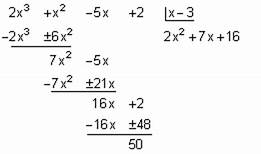
\includegraphics[scale=0.95]{division de polinomios}
\end{center}

\subsubsection*{Teorema de Bezout en polinomios}
Dados dos polinomios con coeficientes en un cuerpo conmutativo, su máximo común divisor se puede expresar como combinación lineal de ambos polinomios.
$$f,g\in \mathbb K[x], d=mcd(f,g)\Rightarrow d=uf+vg : u,v\in \mathbb K[x]$$
Cuando ocurre el caso particular de que $d=1$ entonces los polinomios $u(x)$ y $v(x)$ deben ser constantes no nulas, ya que:
$$1=u(x)\cdot v(x)\Rightarrow gr(1)=gr(u)+gr(v)\Leftrightarrow 0=gr(u)+gr(v)\Rightarrow gr(u)=gr(v)=0 \Rightarrow u=k, v=z : k,z\in \mathbb R$$

\subsection*{\underline{Polinomios primos e irreducibles}}
Decimos que $f\in \mathbb K[x], gr(f)>0$ es \textbf{irreducible} si $f=g\cdot h \Rightarrow gr(g)=0 \vee gr(h)=0$, es decir, $g,h\in \mathbb K[x]^x$\par
Decimos que $f\in \mathbb K[x], gr(f)>0$ es \textbf{primo} si $f|g\cdot h \Rightarrow f|g \vee f|h$, es decir, $g,h\in \mathbb K[x]^x$\par
De ambas definiciones se desprende la siguiente proposición:
$$f\mbox{ primo}\Leftrightarrow f \mbox{ irreducible}$$
\underline{Demostración}:\par
Supongamos que $f$ es irreducible, que $f\mid gh$ y $f\nmid g$
$$mcd(f,g)=1\stackrel{Bezout}{\Rightarrow} 1=uf+vg\Leftrightarrow h=uhf+vgh \stackrel{gh=f\cdot q_1}\Leftrightarrow h=(uh+vq_1)f\Rightarrow f\mid h \Rightarrow p \mbox{ es primo}$$

Supongamos ahora que $f$ es primo, con lo cual:
$$f\mbox{ primo} \Rightarrow f\mid g \vee f\mid h$$
$$f=g\cdot h \Rightarrow 1=q_1(x)\cdot h(x) \Rightarrow gr(1)=gr(q_1)+gr(h)\Rightarrow 0=gr(q_1)+gr(h)\Rightarrow $$
$$\Rightarrow gr(q_1)=gr(h)=0 \Rightarrow \mbox{ son constantes} \Rightarrow f \mbox{ primo}$$

\subsubsection*{Teorema}
Sea $f\in \mathbb K[x]$ y $f$ no constante:
\begin{enumerate}
\item $\exists f_1,f_2, ..., f_n\in \mathbb K[x]$ irreducibles $: f=f_1\cdot f_2 \cdot ... \cdot f_n$

\item Si $f=g_1\cdot g_2 \cdot ... \cdot g_s \in \mathbb K[x]$ también irreducible $\Rightarrow r=s \wedge f_i=a_i\cdot g_i : \forall i=1,...,r$ donde $a_i\in \mathbb K[x]^x$
\end{enumerate}

\underline{Demostración}:

\begin{enumerate}
\item Demostramos la existencia:\par
Sea $f(x)$ un polinomio cualquiera perteneciente a $K[x]$:
$$
\begin{cases}
\mbox{Si }f(x)\mbox{ primo} & \Rightarrow \mbox{Q.E.D.} \\
\mbox{Si }f(x)\mbox{ no primo} & \Rightarrow \exists g(x): g(x)\mid f(x) : gr(g)\mbox{ minimo}\Rightarrow f(x)=g_1(x)\cdot f_1(x)
\end{cases}
$$
Si aplicamos sucesivas veces el caso de los primos, llegará un momento en el que:
$$f=g_1\cdot g_2\cdot g_3 \cdot ... \cdot g_n \cdot f_n$$
Donde $f_n(x)$ será primo y en consecuencia, $f$ será descomposición de polinomios primos.

\item Demostramos la unicidad:\par
Por inducción sobre $r$:
\begin{enumerate}
\item Probamos los casos base: $r=1\Rightarrow f_1=g_1$

\item Demostrados los casos $n\leq r-1$, demostramos que:
$$f_1\cdot f_2 \cdot ... \cdot f_r=g_1\cdot g_2 \cdot ... \cdot g_s \Rightarrow f_1\mid g_1\cdot ... \cdot g_n\Rightarrow f_1\mid g_i \Rightarrow g_1=f_1\cdot h \Rightarrow h=a_0=cte.$$
Sustituyendo en la expresión inicial:
$$f_1\cdot ... \cdot f_r=f_1\cdot a_0\cdot g_2\cdot ... \cdot g_n\Rightarrow f_2\cdot ... \cdot f_r=a_0\cdot g_2\cdot ... \cdot g_s$$
En el primer lado de la igualdad hay $r-1$ factores y en el lado derecho $s-2$, con lo cual:
$$r-1=s-1\stackrel{H.I:}{\Rightarrow }r=s$$
\end{enumerate}
\end{enumerate}

\subsection*{\underline{Raíces de un polinomio}}
Son los valores que hacen 0 el polinomio, pero obsevemos con detenimiento un concepto que tal vez no tengamos en la cabeza de Bachillerato, veamos con detenimiento el siguiente polinomio:
$$f(x)=x^2+1\in \mathbb R[x]$$
Es curioso observar que a priori diríamos que este polinomio no tiene raíces en los $\mathbb R$, pero cojamos la siguiente matriz:
$$A=\left( 
\begin{array}{*2c}
0 & -1 \\
1 & 0 \\
\end{array}
\right)
$$
Ahora el valor del polinomio es:
$$f(A)=A^2+I=\left(\begin{array}{*2c}0 & -1 \\ 1 & 0 \\ \end{array}\right)\cdot \left(\begin{array}{*2c}0 & -1 \\ 1 & 0 \\ \end{array}\right) + \left(\begin{array}{*2c}1 & 0 \\ 0 & 1 \\ \end{array}\right)= \left(\begin{array}{*2c}0 & 0 \\ 0 & 0 \\ \end{array}\right)=0$$
Luego de aquí se desprende que el polinomio tiene raíces en el anillo de las matrices cuadradas, a pesar de que habíamos dicho que no tenía raíces reales.\par
Supongamos que $f\in\mathbb K[x]$ y que $\mathbb K \subset \mathbb F$, siendo ambos cuerpos conmutativos (como $\mathbb R$ y $\mathbb C$, p. ej.), si uno es el subcuerpo del otro, es decir, poseen las mismas operaciones y uno está contenido en el otro, entonces considerando un $\alpha\in \mathbb F$ se define:
$$f(\alpha)=a_0+a_1\alpha+...+a_n\alpha^n$$
En consecuencia, $f(\alpha)\in \mathbb F$ y es ráiz del polinomio $f$ si $f(\alpha)=0$
\subsubsection*{Proposición}
$\alpha$ es raíz de $f\Leftrightarrow f(\alpha)=(x-\alpha)\cdot g(x)$ para algún $g\in \mathbb F[x]$, es decir, las raíces de un polinomio generan factores lineales de un polinomio.\par
\underline{Demostración}:
\begin{enumerate}
\item $\Rightarrow$:\par
Tomamos $f\in \mathbb K[x]\Rightarrow f\in \mathbb F[x]$ y como $\alpha \in \mathbb F[x]\Rightarrow x-\alpha \in \mathbb F[x]$, entonces tenemos que: $f(x)=q(x)(x-\alpha)+r(x): q,r\in \mathbb F[x]$. \par
Llegados a este punto, $r(x)=0\vee gr(r)<gr(x-\alpha)$ siendo $r(x)\neq 0$. Entonces $r(x)=a_0\neq 0$ porque $gr(x-\alpha)=1$, pero como $\alpha$ es raíz:
$$f(\alpha)=0=q(\alpha)\cdot(\alpha-\alpha)+r(\alpha)\Leftrightarrow 0=q(\alpha)\cdot 0+ a_0\Rightarrow a_0=0\Rightarrow r(x)=0$$

\item $\Leftarrow$:\par
$$f(x)=(x-\alpha)g(x)\Rightarrow f(\alpha)=(\alpha-\alpha)g(\alpha)=0\cdot g(\alpha)=0$$
\end{enumerate}

\subsubsection*{Propiedades}
Sean $f=a_0+a_1x+...+a_nx^n$ y $g=b_0+b_1x+...+b_mx^m$ dos polinomios, el producto de polinomios evaluados es equivalente la evaluación del producto y de la suma de polinomios.
$$f(\alpha)+g(\alpha)=(f+g)(\alpha)$$
$$f(\alpha)\cdot g(\alpha)=(f\cdot g)(\alpha)$$ 
\underline{Demostración}\footnote{La demostración de la suma es trivial}:
\begin{itemize}
\item $f(\alpha)+g(\alpha)$:
$$(a_0+a_i\alpha +...+a_n\alpha ^n)(b_0+b_1\alpha +...+b_m\alpha ^m)=\sum_{0\leq i \leq n} (a_i\alpha ^i)(b_j\alpha ^j)=\sum_{0\leq i \leq n\wedge 0\leq j\leq m} (a_ib_j\alpha^{i+j})$$

\item $(f\cdot g)(\alpha)$:
$$\left(\sum_{k=0}^{n+m}\left(\sum_{i+j=k} a_ib_j\right)x^k\right)(\alpha)=\sum_{k=0}^{n+m}\left(\sum_{i+j=k} a_ib_j\right)\alpha^k$$
Y se puede observar que:
$$\sum_{0\leq i \leq n\wedge 0\leq j\leq m} (a_ib_j\alpha^{i+j})=\sum_{k=0}^{n+m}\left(\sum_{i+j=k} a_ib_j\right)\alpha^k$$
\end{itemize}

\subsubsection*{Teorema}
Sea $f\in \mathbb K[x]: \mathbb K\subset \mathbb F \wedge f\neq 0$, el número de raíces del polinomio es menor o igual que el grado del polinomio:
$$|\{\alpha\in \mathbb F: f(\alpha)=0\}|\leq gr(f)$$
\underline{Demostración}:
Razonamos por inducción sobre el $gr(f)=n$:
$$n=0\rightarrow f=a_0\neq 0\Rightarrow \{\alpha \in \mathbb F: f(\alpha)=0\}=\emptyset$$
Tomando como cierta la proposición para los valores inferiores a $n$, demostramos los correspondientes a $n$:
$$gr(f)=n\Rightarrow 
\begin{cases}
\nexists \alpha \in \mathbb F: f(\alpha)=0 & \Rightarrow f(\alpha)\neq 0: \forall \in \mathbb F\Rightarrow 0\leq n \\
\exists \alpha \in \mathbb F: f(\alpha)=0 & \Rightarrow\quad(*) 
\end{cases}$$
$$(*)\rightarrow f(\alpha=0)\Rightarrow f(x)=(x-\alpha)\cdot g(x): g\in \mathbb F[x]\wedge gr(g)=n-1\Rightarrow f(\beta)=0\Leftrightarrow (\beta-\alpha)\cdot g(\beta)=0\Leftrightarrow$$
$$\Leftrightarrow \beta-\alpha=0 \vee g(\beta)=0\Leftrightarrow |\{\beta\in\mathbb F: f(\beta)=0\}|=1+|\{\beta\in\mathbb F: g(\beta)=0\}|\Rightarrow
$$
$$\Rightarrow |\{\beta\in\mathbb F: f(\beta)=0\}|\leq 1+gr(g)=1+n-1$$

\subsection*{\underline{Teorema Fundamental del Álgebra}}
Si $f\in \mathbb C[x]$ y es no constante, entonces $\exists \alpha\in \mathbb C: f(\alpha)=0$.\par
La demostración de dicho Teorema excede con creces la capacidad de este curso así que se pospondrá para más adelante, sin embargo, si podemos demostrar un Corolario:

\subsubsection*{Corolario}
Si $f\in\mathbb R[x]\Rightarrow \exists \alpha \in \mathbb C: f\in \mathbb C[x]\Rightarrow f(\alpha)=0$\par
\underline{Demostración}:\par
Supongamos que $f\in \mathbb C[x]: f=\sum_{i=0}^n a_ix^i: a_i\in \mathbb C$, tomamos su conjugado como $\bar{f}=\sum_{j=0}^n \bar{a_j}x^j: a_j\in \mathbb C$ y, por último, definimos el polinomio $h=f\cdot \bar{f}=\sum_{k=0}^{2n} \left( \sum_{i+j=k}(a_i\bar{a_j}\right) x^k$:
$$\overline{\sum_{i+j=k}(a_i\bar{a_j}})=\sum_{i+j=k}(\bar{a_i}{a_j})\Rightarrow h\in\mathbb R[x]\Rightarrow \alpha\in \mathbb C: 0=h(\alpha)=f(\alpha)\cdot \bar{f}(\alpha)\Rightarrow$$
$$
\begin{cases}
f(\alpha)=0 \\
f(\alpha)\neq 0\Rightarrow \bar{f}(\alpha)=0\Rightarrow \overline{\bar{f}(\alpha)}=0\Rightarrow 0=\overline{\sum_{i=0}^n(\bar{a_i}\alpha^i)}=\sum_{i=0}^n(a_i\bar{\alpha}^i)=f(\bar{\alpha})=0
\end{cases}
$$

\subsection*{\underline{Teorema de la irreducibilidad de un polinomio}}
Un polinomio $f\in \mathbb C[x]$ es irreducible cuando $gr(f)=1$, puesto que ya hemos comprobado que para $gr(f)>1$, $f$ posee tantas raíces como el valor del grado del polinomio y  cada raíz descompone el polinomio en un factor lineal.

\subsubsection*{Corolario}
$$f\in \mathbb C[x]: gr(f)=n\geq 1\Rightarrow \exists!\alpha_1,...,\alpha_n, a\in \mathbb C: a\neq 0: f(x)=a(x-\alpha_1)\cdot ...\cdot (x-\alpha_n)$$

\subsubsection*{Polinomios irreducibles en $\mathbb R$}
Para un $f\in \mathbb R[x]$, es irreducible si y solo si $gr(f)=1$ $gr(f)=2$ y su discriminante es negativo.
\underline{Demostración}:
\begin{itemize}
\item ``$\Rightarrow$''
$$\frac{-b\pm \sqrt{\Delta}}{2a}\notin \mathbb R : \forall \Delta <0$$

\item ``$\Leftarrow$'': $f\in \mathbb R[x]\mbox{ irreducible}: gr(f)>1\Rightarrow$
$$\exists \alpha\in \mathbb C: f(\alpha)=0\Rightarrow f(\bar{\alpha})=0\Rightarrow f(x)=(x-\alpha)(x-\bar{\alpha})h(x): h(x)\in \mathbb C[x]$$
Por lo tanto como:
$$f(x)=(x^2-2Real(\alpha)x+|\alpha|^2)h(x)$$
Descompone en división exacta con $h(x)$ si este es no constante, pero como ambas raíces pertenecen a los complejos, cuando $h(x)$ es constante, es irreducible en $\mathbb R$ con grado 2.
\end{itemize}

De estos hechos se deduce que TODO polinomio impar SIEMPRE es irreducible, porque pueden ser producto de uno de grado 1 y otro de grado 2 o 3 de grado 1.

\subsubsection*{Polinomios irreducibles en $\mathbb Q$}
En este conjunto podemos encontrar polinomios irreducibles de cualquier grado, pero existe un teorema conocido como \textbf{criterio de Einsenstein} que dice:
$$\exists p\mbox{ primo}\in \mathbb Z: p\mid a_0, p\mid a_1,..., p\mid a_{n-1}\wedge p\nmid a_n \wedge p^2\nmid a_0\Rightarrow f\mbox{ es irreducible}$$
Para calcular dichas raíces podemos buscar un $\alpha=\frac{r}{s}\in \mathbb Q: r\mid a_0\wedge s\mid a_n$. Además se puede añadir como criterio\footnote{La demostración de este añadido se hizo en un ejercicio que no figura en el documento} $r-s\mid p(1)$ y $r+s\mid p(-1)$\par
\underline{Demostración}:
Aplicamos que es una raíz:
$$0=a_0+a_1\frac{r}{s}+...+a_n\frac{r^n}{s^n}\stackrel{\cdot s^n}{\Rightarrow}0=a_0s^n+a_1rs^{n-1}+...+a_{n-1}r^{n-1}s+a_nr^n\stackrel{1.)2.)}{\Rightarrow}$$
$$\mbox{1.)}\rightarrow -a_0s^n=(a_1s^{n-1}+...+a_nr^{n-1})r\Rightarrow r\mid -a_0s^n\Rightarrow r\mid a_0$$
$$\mbox{2.)}\rightarrow -a_nr^n=(a_0s^n+...+a_nr^{n})s\Rightarrow s\mid -a_nr^n\Rightarrow s\mid a_n$$

\subsubsection*{Polinomios irreducibles en $\mathbb Z_p$}
Siempre que tengamos un cuerpo conmutativo hay polinomios irreducibles de cualquier grado.\par
Ej.: $f\in \mathbb Z_2[x]$
\begin{itemize}
\item Grado 1: $x+1$, $x$ irreducibles
\item Grado 2: $x^2$, $x^2+x$, $x^2+1$ no son irreducibles pero $x^2+x+1$ sí
\item ...
\end{itemize}

\subsection*{\underline{Teorema raíces en una extensión de K}}
Existe un teorema que dice que si extendemos K a un cuerpo superior que lo contenga, entonces podemos encontrar ahí también las raíces de un polinomio de $K[x]$, pero antes vamos a ver determinados ejemplos.

\subsubsection*{Ejemplo 1}
Si definimos la matriz $C\in Mat_n(\mathbb K$ y definimos $f(C)$ como la evaluación de $f$ en $C$, siendo:
$$C=\left(\begin{array}{ccc}
0 & 0 & -1 \\
1 & 0 & -1 \\
0 & 1 & 0
\end{array}\right)\stackrel{\mathbb Z_2}{=}
\left(\begin{array}{ccc}
0 & 0 & 1 \\
1 & 0 & 1 \\
0 & 1 & 0
\end{array}\right)
$$
$$f(x)=x^3+x+1\rightarrow \mbox{irreducible en }\mathbb Z_2$$
Ahora podemos decir que $f(C)=C^3+C+I=0$, extendiendo un polinomio irreducible en K, a un anillo que contiene a K y donde no es irreducible.\par
Para formalizar el cuerpo al que debe pertenecer esta raíz, lo definimos de la siguiente manera:
$$F=\{g(C): g\in \mathbb Z_2[x]\}\subseteq Mat_3(\mathbb Z_2)$$
Las matrices que conforman este nuevo cuerpo son: $\{a_0I, a_0I+a_1C, a_0I+a_1C+a_2C^2,...\}$. Para comprobar que es un cuerpo definimos la suma y el producto de los elementos de dicho conjunto:
$$g(C)+h(C)=(g+h)(C)\in F$$
$$g(C)\cdot h(C)=(g\cdot h)(C)\in F$$
Con esta definición podemos decir que $(F,+,\cdot)$ es un cuerpo conmutativo con 8 elementos, y por tanto $\mathbb Z_2\subset F$.\par
\underline{Demostración}:
$$+:\mbox{asociativa, elemento neutro: }0=0(C)\in F, \mbox{ elemento opuesto: } -g(C)=(-g(C)\in F\mbox{ y es conmutativa}$$
$$\cdot: \mbox{asociativa, distributiva, elemento neutro: }1(C)=I\in F,\mbox{ conmutativa}$$\footnote{$g(C)\cdot h(C)=(g\cdot h)(C)=(h\cdot g)(C)=h(C)\cdot g(C)$}
Con  cual tras demostrar todas estas propiedades, podemos decir con seguridad que es un anillo conmutativo y unitario. Para ver que es un cuerpo:
$$g(C)\neq 0\in F\Rightarrow g\neq 0\wedge x^3+x+1\nmid g\mbox{ porque si lo hiciese }g(C)=(C^3+C+I)h(C)=0\mbox{ \#}$$
$$\mbox{Además }mcd(x^3+x+1,g)=1\Rightarrow 1=k(x)(x^3+x+1)+h(x)g(x)\Rightarrow I=k(C)\cdot 0+h(C)g(C)=h(C)g(C)$$
$$\Rightarrow h(C)=g^{-1}(C)$$
Por último\footnote{Decir que un cuerpo es isomorfo a otro ``$\simeq$'', es decir que existe una biyección entre ambos conjuntos que conserva la suma y el producto}, $ Z_2 \simeq \{a_0I: a_0\in \mathbb Z_2\}\subset F$

\underline{Por qué tiene 8 elementos?}:
$$g(C)=[q(x)(x^3+x+1)+r(x)](C)=q(C)\stackrel{=0}{(C^3+C+I)}+r(C)=r(C)$$
Por lo que:
$$C\subset F=\{g(C): g\in \mathbb Z_2[x]\}=\{a_0I+a_1C+a_2C^2: a_0,a_1,a_2\in \mathbb Z_2\}$$

\subsubsection*{Teorema de extension de K cuando f es irreducible}
De este ejemplo nace el caso general del teorema que dice: ``Para cualquier polinomio puedes encontrar raíces en un cuerpo que sea extensión del cuerpo en el que está definido''.\par
Sean:
$$f=x^n+a_{n-1}x^{n-1}+...+a_1x+a_0: n\geq 1$$
$$F=\{g(C): g\in K[x]\}$$
$$C=\left(\begin{array}{ccccc}
0 & 0 & \cdots & 0 & -a_0 \\
1 & 0 & \cdots & 0 & -a_1 \\
0 & 1 & \cdots & 0 & -a_0 \\
\vdots & \vdots & \ddots & \vdots & \vdots \\
0 & 0 & \cdots & 1 & -a_{n-1}\\
\end{array}\right)$$

Se cumplen las siguientes condiciones:
\begin{enumerate}
\item $f(C)=0: C\in F$
\item $g\neq 0 \wedge gr(g)<gr(f): g\in K[x]\Rightarrow g(C)\neq 0$
\item $(F,+,\cdot)$ es un \textbf{anillo conmutativo y unitario}, y si $f$ es irreducible entonces es un \textbf{cuerpo conmutativo}
\item $K\simeq \{a\cdot I: a\in K\}\subset F$
\item $F=\{g(C): g\in K[x], gr(g)<n\}=\{a_0I+a_1C+...+a_nC^{n-1}: a_0,...,a_{n-1}\in K\}$
\end{enumerate}

\underline{Demostración}:
\begin{enumerate}
\item Suponemos que :
$$C=x(C): x\in K[x]\Rightarrow C\in F$$
Llegados a este punto si llamamos $A=f(C)$ tratamos de demostrar que $A=0$:
$$A=0\Rightarrow A\cdot I=0\Leftrightarrow \begin{cases}
A\cdot E_1=0 \\
A\cdot E_2=0 \\
\vdots \\
A\cdot E_n=0
\end{cases}$$
Donde $E_i$ denota a cada una de las columnas de la matriz identidad. De este modo deducimos que:
$$A\cdot E_1=(a_0+a_1C+\cdots +a_{n-1}C^{n-1}+a_nC^n)E_1=a_0E_1+a_1CE_1+\cdots +a_{n-1}C^{n-1}E_1+a_nC^nE_1=$$
$$\stackrel{CE_i=E_{i+1}}=a_0E_1+a_1E_2+\cdots +a_{n-1}E_n+(-a_0E_1-a_1E_2-\cdots -a_{n-1}E_n)=0$$
Para demostrar el resto de casos, basta con observar que:
$$A\cdot E_2=A\cdot C\cdot E_1=(a_0I+a_1C+\cdots+ a_{n-1}C^{n-1}+C^n)CE_1\stackrel{C\cdot C^{i}}{=}C\cdot A\cdot E_1=C\cdot 0=0$$

\item Como $g\neq 0\Rightarrow g=b_0+\cdots+b_mx^m: \exists b_i\neq 0$ y desde aquí deducimos que:
$$0=g(C)=b_0I+b_1+\cdots +b_mC^m\stackrel{\cdot E_1}{\Rightarrow} 0=b_0IE_1+b_1CE_1+\cdots+b_mC^mE_1\Rightarrow$$
$$\Rightarrow \left(\begin{array}{c}
b_0 \\
b_1 \\
\vdots \\
b_m \\
0 \\
\vdots \\
0
\end{array}\right)=0\Rightarrow \mbox{ \#, Porque para que sea no nulo, algún $b_i$ debe ser distinto de 0.}
$$

\item Que las propiedades de ser anillo conmutativo y unitario son demostraciones triviales, sin embargo, la demostración de que cuando $f$ es irreducible, $F$ adquiere las propiedades de cuerpo reviste más importancia y complejidad:
$$0\neq g(C)\in F\Rightarrow f\nmid\Rightarrow mcd(f,g)=1\Rightarrow$$
$$\Rightarrow 1=u(x)f(x)+h(x)g(x)=u(C)f(C)+h(C)g(C)=h(C)g(C)\Rightarrow g^{-1}(C)=h(C)$$

\item Al ser un subcuerpo:
\begin{gather*}
aI+bI=(a+b)I\in F \\
(aI)(bI)=(ab)I\in F \\
0=0I\in F \\
I=1\cdot I\in F \\
-(aI)=(-a)I\in F \\
(aI)^{-1}\stackrel{a\neq 0}{=}a^{-1}I \\
\end{gather*}

Por ser un isomorfismo:
$$K\stackrel{\phi}{\rightarrow}\{aI: a\in K\}$$
Observamos que la función $\phi$ es claramente biyectiva y como $\phi(a+b)=(a+b)I=aI+bI=\phi(a)+\phi(b)$ y $\phi(a\cdot b)=(a\cdot b)I=aI\cdot bI=\phi(a)\cdot \phi(b)$, se ve que se conserva la suma y el producto por lo tanto podemos decir que $K\simeq \{aI: a\in K\}\subset F$
\vspace{0.5cm}
\item Suponemos un $g(x)\in K[x]$, podemos decir por el Teorema de la división entera que $g=f\cdot q + r$, donde $r=0$ o $gr(r)<n$, esto implica que $g(C)=f(C)q(C)+r(C)=r(C)$ porque $f(C)=0$ así que: $gr(g)=gr(r)<gr(f)$
\end{enumerate}

\subsubsection*{Caso interesante}
Un caso interesante de la posible aplicación de este teorema es la qeu sigue, sea $f=x^2+1\in \mathbb R[x]$ y $F=\{a_0I+a_1C: a_0,a_1\in \mathbb R\}$, donde $C\left(\begin{array}{cc} 0 & -1 \\ 1 & 0 \end{array}\right)$.\par
En consecuencia, si hallamos una expresión general de las matrices que pertenecen al cuerpo F, estas son de la forma $\left(\begin{array}{cc}a_0 & -a_1 \\ a_1 & a_0\end{array}\right)$. De esta forma observamos que la información general de la matriz esta contenida en la 1ª columna puesto que conocida la primera columna conocemos el resto de la matriz. Si consideramos que dos matrices distintas de F, su producto tiene el siguiente aspecto:
$$\left(\begin{array}{cc}a_0 & -a_1 \\ a_1 & a_0\end{array}\right)\cdot \left(\begin{array}{cc}b_0 & -b_1 \\ b_1 & b_0\end{array}\right)=\left(\begin{array}{cc}a_1b_0-a_1b_1 & \cdots \\ a_1b_0+a_0b_1 & \cdots \end{array}\right)$$
Con lo cual se puede apreciar que si solo nos fijamos en la primera columna, se puede usar este cuerpo F como un buen modelo de los \textbf{números complejos} porque de hecho, la matriz $C$ compañera del polinomio $f$ es, según esta interpretación, el número $i$ y si nos fijamos en sus elementos coincide con lo relatado.
\subsubsection*{Para el caso del otro día}
$$f=x^3+x+1\in \mathbb Z_2\Rightarrow F=\{a_0I+a_1C+a_2C^2: a_0,a_1,a_2\in \mathbb Z_2\}\mbox{ donde } C=\left(\begin{array}{ccc} 0 & 0 & -1 \\ 1 & 0 & -1 \\0 & 1 & 0 \end{array}\right)\stackrel{\mathbb Z_2}{=}\left(\begin{array}{ccc} 0 & 0 & 1 \\ 1 & 0 & 1 \\0 & 1 & 0 \end{array}\right)$$
$$\mbox{Las matrices de F son: }\left(\begin{array}{ccc} a_0 & 0 & 0 \\ 0 & a_0 & 0 \\0 & 0 & a_0 \end{array}\right)+\left(\begin{array}{ccc} 0 & 0 & a_1 \\ a_1 & 0 & a_1 \\0 & a_1 & 0 \end{array}\right)+\left(\begin{array}{ccc} 0 & a_2 & 0 \\ 0 & a_2 & a_2 \\a_2 & 0 & a_2 \end{array}\right)$$

\subsubsection*{Teorema de extensión de K para cualquier polinomio}
Como consecuencia del teorema que se cumple para los polinomios irreducibles, podemos extender su enunciado al TODOS LOS POLINOMIOS, con independencia de su irreducibilidad.\par
El teorema dice: sea $f\in K[x]$ no constante, entonces $\exists F\supset K$, un $a\in K$ y $\alpha_1, ..., \alpha_n\in F$ tales que:
\begin{enumerate}
\item $F$ es un cuerpo conmutativo que contiene a K como subcuerpo.
\item $f(x)=a(x-\alpha_1)\cdot ... \cdot (x-\alpha_n)$
\end{enumerate}

\underline{Demostración}: por inducción sobre $n=gr(f)$:
\begin{itemize}
\item Caso base:$n=1$
$$f(x)=a_1x+a_0: a_0,a_1\in K\wedge a_1\neq 0\Rightarrow F=K\wedge \alpha_1=-a_0\cdot a_1^{-1}\in K\wedge a=a_1$$
\item Paso inductivo, consideramos cierto para $l<gr(f)=n$:
$$f=p_1\cdot ... \cdot p_m: p_i\in K[x] \mbox{ irreducible}\Rightarrow p_i\in K\Rightarrow K\subset K_1 \wedge \alpha_1\in K: p(\alpha_1)=0\Rightarrow$$
$$\Rightarrow f(\alpha_1)=0\Rightarrow f(x)=(x-\alpha_1)g(x)\mbox{ donde }g(x)\in K[x]: gr(g)=l\stackrel{H.I.}{\Rightarrow}$$
$$K\subset K_1\subset F: g(x)=a(x-\alpha_2)\cdot ...(x-\alpha_n)\Rightarrow f(x)=a(x-\alpha_1)(x-\alpha_2)\cdot ... \cdot (x-\alpha_n)\in F$$
\end{itemize}

\subsection*{\underline{Relaciones de Girard-Newton}}
Al analizar el grado de un polinomio cuadrático mónico cualquiera como $f=a_0+a_1x+x^2$, se observa que el número de raíces según lo hablado en el capítulo debería ser 2, de este modo, el polinomio se puede reescribir como: $f=(x-\alpha_1)(x-\alpha_2)$. Desarrollando:
$$f=(x-\alpha_1)(x-\alpha_2)=x^2-(\alpha_1+\alpha_2)x+\alpha_1\alpha_2\Rightarrow\begin{cases}a_0=\alpha_1\cdot \alpha_2 \\
a_1=-(\alpha_1+\alpha_2)\end{cases}$$
De este razonamiento para el caso de un polinomio de grado 2, se desprenden \textbf{las relaciones de GIRARD-NEWTON\footnote{Guardan relación con las fórmulas de generación de los polinomios simétricos elementales}}, que son generales para cualquier grado.
$$a_{n-k}=(-1)^k\cdot \sum_{1\leq i\leq \cdots \leq i_k<n}\alpha_{i_1}\cdot ... \cdot \alpha_{i_k}\mbox{ donde }k=0,1,2, ..., n$$
Ej\footnote{En el fondo se trata de hacer sumandos de $n-k$ elementos y poner tantos sumandos como posibles combinaciones de raíces}:
$$n=3\rightarrow \begin{cases} a_0=-\alpha_1\alpha_2\alpha_3 \\
a_1=\alpha_1\alpha_2+ \alpha_1\alpha_3+ \alpha_2\alpha_3 \\
a_2=-(\alpha_1+\alpha_2+\alpha_3)
\end{cases}$$
Estas relaciones nos otorgan la capacidad manifiesta de poder  construir polinomios a partir de otros sin saber verdaderamente cuales son las raíces de los de partida:
$$\mbox{Sea }p(x)=x^3+3x+1\Rightarrow p(x)=(x-\alpha_1)(x-\alpha_2)(x-\alpha_3)\Rightarrow
\begin{cases}
a_0=1=-\alpha_1\alpha_2\alpha_3 \\
a_1=3=\alpha_1\alpha_2+\alpha_1\alpha_3+\alpha_2\alpha_3 \\
a_2=1=-(\alpha_1+\alpha_2+\alpha_3)
\end{cases}$$
Aunque no conocemos el valor de las raíces, si que podemos construir un polinomio sabiendo la relación que guardan:
$$\alpha_k'=\alpha_k+1\mbox{ donde }k=1,2,3\Rightarrow$$
$$\Rightarrow p'(x)=x^3+a_2x^2+a_1x+a_0\Rightarrow
\begin{cases}
a_0'=-(\alpha_1+1)(\alpha_2+1)(\alpha_3+1)=-3 \\
a_1'=(\alpha_1+1)(\alpha_2+1)+(\alpha_1+1)(\alpha_3+1)+(\alpha_2+1)(\alpha_3+1)=6 \\
a_2'=-(\alpha_1+\alpha_2+\alpha_3+3)=-3
\end{cases}$$

\chapter*{ESPACIOS VECTORIALES Y \\APLICACIONES LINEALES}
\section*{ESPACIOS VECTORIALES}
Si suponemos que $(V,+,\cdot)$ donde $+: V\times V\rightarrow V$ y $\cdot : K\times V\rightarrow V$, siendo $K$ un cuerpo conmutativo y a esta terna se le conoce como \textbf{ESPACIO VECTORIAL} sobre $K$ si:
\begin{itemize}
\item $(V,+)$ es un grupo conmutativo (existe el elemento neutro $0_v$ y todos tienen opuesto $-v$).

\item $\forall a \in K: \forall v,v'\in V: a(v+v')=av+av'$

\item $\forall a,a' \in K: \forall v\in V: (a+a')v=av+a'v$

\item $\forall a,a'\in K: \forall v \in V: a(a'v)=(aa')v$

\item $\forall v\in V: 1_k\cdot v=v$
\end{itemize}
A los elementos de este conjunto conocido como espacio vectorial los llamaremos \textbf{vectores}.

\subsubsection*{Propiedades}
Algunas propiedades muy elementales\footnote{Cuando en un anillo se dice que no hay divisores de 0 decimos que es un anillo de integridad, por ejemplo, $\mathbb Z$}:
\begin{enumerate}
\item $a,b\in K: ab=0_k\Rightarrow a=0_k \vee b=0_k$

\item $a\cdot 0_k=0_k$

\item $0_k\cdot v=0_v$ y $a\cdot 0_v=0_v$

\item $a\cdot v=0_v\Rightarrow a=0_k \vee v=0_v$
\end{enumerate}

\underline{Demostraciones}:
\begin{enumerate}
\item 
$$ab=0_k\wedge a\neq 0_k\Rightarrow \exists a^{-1}\in K\Rightarrow a^{-1}ab=a^{-1}0\Rightarrow b=0_k\Rightarrow \mbox{No hay divisores de 0}$$

\item
$$a\cdot 0_k=a\cdot (0_k+0_k)=a\cdot 0_k+a\cdot 0_k\stackrel{-a\cdot 0_k}{\Leftrightarrow}a\cdot 0_k-a\cdot 0_k=a\cdot 0_k+a\cdot 0_k-a\cdot 0_k\Leftrightarrow 0_k=a\cdot 0_k$$

\item
$$0_k\cdot v=(0_k+0_k)v=0_kv+0_kv\stackrel{-0_kv}{\Leftrightarrow} 0_kv-0_kv=0_kv+0_kv-0_kv\Leftrightarrow 0_v=0_kv$$

\item
$$av=0_v\wedge a\neq 0_k\stackrel{\exists a^{-1}}{\Rightarrow} a^{-1}av=a^{-1}0_v\Leftrightarrow (a^{-1}a)v=0_v\Leftrightarrow v=0_v$$
\end{enumerate}

\subsubsection*{Ejemplos representativos}
Veamos algunos ejemplos de espacios vectoriales:\par
Suponemos $V=K^n=K\times ... \times K \mbox{ (n veces)}$, tenemos que definir ahora la suma de dos vectores y el producto por un escalar:
 $$(a_1, ..., a_n)+(b_1, ..., b_n)=(a_1+b_1, ..., a_n+ b_n)$$
 $$a(a_1, ..., a_n)=(a\cdot a_1, ..., a\cdot a_n)$$
Está claro que existe el neutro de la suma $0_v=(0,...,0)$ y que existe el opuesto $-(a_1, ..., a_n)=(-a_1, ..., -a_n)$. Demostramos por ejemplo alguna de las propiedades definidas al principio:
$$(ab)(a_1, ..., a_n)=(aba_1, ..., aba_n)=a(ba_1, ..., ba_n)$$
Este ejemplo que hemos dado es el enésimo espacio vectorial estándar o canónico, y probaremos más adelante que cualquier espacio vectorial es isomorfo\footnote{Cuando $n=1$, hablamos de la recta vectorial; cuando $n=2$, del plano y cuando $n=3$ del espacio vectorial} a este y, por tanto, es modelo de los demás.\par

\vspace{0.35cm}

Veamos otro ejemplo:\par
Consideramos $V=K[x]$ y definimos la suma y el producto por un escalar:
$$f+g\mbox{ es la suma habitual de polinomios}$$
$$a\cdot f=b\sum_{i=0}^n a_ix^i=\sum_{i=0}^n (b\cdot a_i)x^i$$
Se pueden comprobar a través de esta definición el resto de propiedades de espacio vectorial confirmando que se puede considerar como el mismo.

\vspace{0.35cm}

Veamos otro ejemplo:\par
Llamamos $W=K_n[x]=\{f\in K[x]: gr(f)<n\}$, pues definidas las operaciones anteriores\footnote{W es un subespacio vectorial de V} también cumple las propiedades de espacio vectorial, además, se comprueba fácilmente que el producto y la suma de polinomios definidas antes conservan que todo polinomio del conjunto tras ser operado con otro tenga como resultado un polinomio del conjunto (no altera el grado), por lo tanto es cerrado.\par

\vspace{0.35cm}

Veamos otro ejemplo:\par
Llamamos $V=Mat_{m\times n}(K)$, se definen la suma y el producto como:
$$(a_{ij})+(b_{ij})=(a_{ij}+b_{ij})$$
$$b(a_{ij})=(b\cdot a_{ij})$$
Y del mismo modo se pueden comprobar todas las propiedades anteriores para confirmar que se trata realmente de un espacio vectorial.

Veamos otro ejemplo:\par
Llamamos $V=\{f: \mathbb R\rightarrow \mathbb R: f \mbox{ es una aplicación}\}$, definimos suma y producto:
$$(f+g)(x)=f(x)+g(x):\forall x \in \mathbb R\mbox{ y se puede comprobar que eso es un grupo conmutativo}$$
$$(a\cdot f)(x)=a\cdot f(x)$$
Y del mismo modo, se puede comprobar que esta definición cumple todas las propiedades de espacio vectorial.

\subsection*{\underline{Subespacios vectoriales}}
Siendo $V$ un espacio vectorial sobre un cuerpo $K$ y $W\subseteq V: W\neq 0$, se dice que $W$ es un \textbf{subespacio vectorial} de $V$ si:

\begin{itemize}
\item $w, w'\in W: w+w'\in W$

\item $a\in K\wedge w\in W: a\cdot w\in W$
\end{itemize}

Veamos que como $W\subseteq V \Rightarrow w\in W\subseteq V$ por lo que se cumplen las propiedades de la definición de espacio vectorial.\par

\textbf{Ej.:} sea $F(\mathbb R, \mathbb R)=\{f:\mathbb R\rightarrow \mathbb R \mid f\mbox{ es aplicacion}\}=V$ espacio vectorial. Si llamamos $W=\{f\in V: f(-x)=f(x): \forall x \in \mathbb R\}$ entonces podemos comprobar que se dan las condiciones de subespacio:
$$f,g\in\mathbb W: (f+g)(-x)=f(-x)+g(-x)=f(x)+g(x)=(f+g)(x)$$
$$a\in \mathbb K, g\in\mathbb W: (a\cdot g)(-x)=a\cdot g(-x)=a\cdot g(x)=(a\cdot g)(x)$$

Dos casos muy concretos\footnote{Es útil pensar que si $W_1$ es el eje x y $W_2$ es el eje y, entonces la union de ambos no es subconjunto del plano porque la suma de vectores de cada eje da vectores del plano}:
$$W_1,W_2 \stackrel{subespacio}{<} V\Rightarrow \begin{cases}
W_1\cap W_2< V \\
W_1\cup W_2\nless V \mbox{ en general} \\
W_1+W_2=\{w_1+w_2: w_1\in W_1\wedge w_2\in W_2\}< V
\end{cases}$$

\subsubsection*{Espacio de generadores: dependencia e independencia lineal}
Primero debemos definir el concepto de independencia y dependencia lineal, un conjunto de vectores $\{v_1, v_2, ..., v_n\}$ es \textbf{linealmente independiente} si toda combinación lineal de ellos nula implica que dichos coeficientes son todos nulos:
$$\forall a_1, ..., a_m\in K: a_1v_1+\cdots +a_mv_m=0_v\Rightarrow a_1=a_2=\cdots =a_m=0$$

Cuando esta condición no se verifica entonces decimos que el conjunto es \textbf{linealmenten dependiente} y entonces cumple que hay una combinación con algún coeficiente no nulo:
$$\forall a_1, ..., a_m\in K: \exists a_1v_1+\cdots +a_mv_m=0_v: \exists a_i\neq 0$$
Esto implica que el vector $v_i$ se puede reescribir como combinación lineal de los restantes:
$$v_i=-a_i^{-1}a_1v_1-...-a_i^{-1}a_{i-1}v_{i-1}-...-a_i^{-1}a_mv_m$$

\textbf{Ej.:} $K\times K\rightarrow K^2$, si tomamos como vectores $e_1=(1,0)$ y $e_2=(0,1)$, estos son linealmente independientes porque:
$$a_1\cdot e_1+a_2\cdot e_2=(0,0)\Leftrightarrow (a_1,a_2)=(0,0)\Leftrightarrow a_1=a_2=0$$
Pero si añadimos el vector $v=(1,-2)$, entonces:
$$-1\cdot e_1+ 2\cdot e_2+ 1\cdot v=(0,0)$$
Lo que resulta en que $\{e_1, e_2, v\}$ son linealmente dependientes.

\subsubsection*{Sistema de generadores}
Sea $S\{v_1, ..., v_m\}$ un conjunto de vectores cuales quiera de la base vectorial $V$, llamamos $L(S)=\{a_1v_1+\cdots + a_mv_m: a_1, ..., a_m\in K\}$ al conjunto de todas las posibles combinaciones lineales de dichos vectores, que también forma un subespacio vectorial. Tenemos por la fuerza que $S\subset L(S)$ y además este conjunto es el menor subespacio vectorial en $V$ que contiene a $S$ y además, para cualquier subespacio vectorial $F\subset V$ que contenga a $S$, este debe contener a $L(S)$.\par
Si $L(S)=F$ decimos que $L(S)$ es un \textbf{sistema de generadores} de $F$ porque es capaz de generarlo.\par
\textbf{Ej.:} $K^2$, si tomamos como $L(e_1,e_2)$ tenemos que $a_1e_1+a_2e_2=(a_1, a_2)\Rightarrow V=L(S)$, luego es generador del espacio vectorial $V$.

\subsection*{\underline{Base vectorial}}
Un espacio vectorial es \textbf{finitamente generado} si su sistema generador está formado por un conjunto finito de vectores: $V=L(S): S=\{v_1, ..., v_m\}: v=a_1v_1+ ... + a_mv_m$. Por ejemplo, $K^2$ es f.g. pero $K[x]$ no lo es.\par

Cuando un conjunto de vectores es \textbf{linealmente independiente} y a su vez \textbf{sistema generador}, decimos que un conjunto $B\subset V$ es base vectorial de $V$. Los vectores de $V$ por tanto se puede expresar como:
$$v=a_1v_1+...+a_mv_m=a_1'v_1+...+a_m'v_m: v_1, ..., v_m\in B$$
De hecho esta descomposición es única porque restando ambas ecuaciones tenemos que:
$$0_v=(a_1-a_1')v_1+...+(a_m-a_m')v_m\stackrel{l.i.}{\Rightarrow} a_1-a_1'=...=a_m-a_m'=0\Rightarrow a_i=a_i'$$

Por ejemplo, en $K^n$, llamamos a $B_c=\{e_1, ..., e_n\}$ su base canónica. En otro caso, $K[x]$ no es finitamente generado, su base es infinita siendo una de ellas: $B=\{1, x, x^2, ...\}$. En un último ejemplo, tenemos que las matrices $Mat_{3\times 2}(K)$ podemos definir la base de esta como: $B=\left\lbrace\left(\begin{array}{cc}1 & 0 \\ 0 & 0 \\ 0 & 0 \end{array}\right), \left(\begin{array}{cc}0 & 1 \\ 0 & 0 \\ 0 & 0 \end{array}\right), \left(\begin{array}{cc}0 & 0 \\ 1 & 0 \\ 0 & 0 \end{array}\right), \left(\begin{array}{cc}0 & 0 \\ 0 & 1 \\ 0 & 0 \end{array}\right), \left(\begin{array}{cc}0 & 0 \\ 0 & 0 \\ 1 & 0 \end{array}\right), \left(\begin{array}{cc}0 & 0 \\ 0 & 0 \\ 0 & 1 \end{array}\right)\right\rbrace$

\subsubsection*{Proposición}
Un conjunto $B$ es base $\Leftrightarrow$ si es un sistema de generadores \textbf{minimal}\footnote{Cuando ningún subconjunto de $B$ es sistema de generadores.}\par
\underline{Demostración}:
\begin{itemize}
\item ``$\Rightarrow$'':
	Supongamos que $B$ no es minimal, entonces $\exists S\subsetneq B: S$ es sistema de generadores:
	$$\exists v\in B: v\notin S: v=a_1v_1+...+a_mv_m: v_n, ..., v_m\in S\Rightarrow 0_v=1_kv-a_1v_1-...-a_mv_m\Rightarrow B\mbox{ no es l. i.}$$
	
\item ``$\Leftarrow$'':
	Supongamos que $B$ no es l.i., entonces $\exists v_1, ..., v_m\in B: a_1v_1+...+ a_mv_m=0_v\Rightarrow$
	$$\Rightarrow \exists i: a_i\neq 0_k\stackrel{p.ej.}{\Rightarrow}a_m\neq 0\Rightarrow v_m=-a_m^{-1}a_1v_1-...-a_m{-1}a_{m-1}v_{m-1}\Rightarrow S=B\mbox{\textbackslash}\{v_m\} \mbox{ es sistm. gen.}\Rightarrow \#$$
Porque entonces $B$ no es minimal.
\end{itemize}

\subsubsection*{Proposición}
Un conjunto $B$ es base $\Leftrightarrow$ si es un linealmente independiente \textbf{maximal}\footnote{Cuando cualquier conjunto que lo contiene no es linealmente independiente.}.\par

\subsubsection*{Teorema}
Todo espacio vectorial finitamente generado tiene alguna base.\par
\underline{Demostración}:\par
Como $V$ es finitamente generado, entonces: $\exists S=\{v_1, ..., v_m\}$ sistema de generadores de $V$ y entonces $\exists S'\subseteq S: S'$ es sistema de generadores minimal, por lo que $S'$ es base. Esto es así porque si a un sistema de generadores se le puede quitar un elemento, entonces no es minimal y puede encontrarse en él uno que sí lo sea, entonces dicho sistema minimal ya es base.\par

Algunos Ejemplos:
$$V=\{0_v\}\Rightarrow B=\emptyset$$
$$V\neq \{0_v\}\Rightarrow L(S)=\{v\}\mbox{ es siempre linealmente independiente}$$

\subsubsection*{Lema de Intercambio}
Supongamos $V$ un espacio finitamente generado y sea $L=\{v_1, ..., v_s\}$ linealmente independiente y $S=\{w_1, ..., w_t\}$ un sistema de generadores. Se cumple que:
\begin{enumerate}
\item $s\leq t$
\item $\exists 1\leq i_1<...< i_s\leq t: \{v_1, ..., v_s\}\cup S\mbox{\textbackslash}\{w_{i_1}, ..., w_{i_s}\}$ es un sistema de generadores.
\end{enumerate}
Lo que viene a afirmar que dado un sistema de generadores, si se sustituyen vectores del mismo por vectores de un conjunto que sea linealmente independiente, entonces el resultado sigue siendo sistema de generadores.

\underline{Demostración}: por inducción sobre $s$:
$$s=1\rightarrow 0\neq v_1: L\{v_1\}\mbox{es l. i. y }S=\{w_1, ..., w_t\}$$
Como S es un sistema de generadores:
$$v_1=a_1w_1+...+a_tw_t\neq 0\Rightarrow \exists a_i\neq 0\stackrel{p.ej.}{\Rightarrow} a_1\neq 0\stackrel{\exists a_1^{-1}}{\Rightarrow} w_1=a_1^{-1}v_1-a_1^{-1}a_2w_2-...- a_1^{-1}a_tw_t\Rightarrow $$
$$\Rightarrow \{v_1, w_2, w_3, ..., w_t\}\mbox{ es sist. gen.}$$

Paso inductivo: cierto para $s-1$, demostramos para s:
$$L\{v_1, ..., v_s\} \mbox{ l. i. y } S=\{w_1, ..., w_t\}$$
$$\{v_1, ..., v_{s-1}\}\mbox{ es l.i.}\Rightarrow \{v_1, ..., v_{s-1},w_s, ...,w_t\}\mbox{ es sistema de generadores}$$
$$v_s=a_1v_1+...+ a_{s-1}v_{s-1}+a_sw_s+...+a_tw_t\neq 0\Rightarrow \exists a_i\neq 0$$
Para demostrarlo, supongamos que $a_s=...=a_t=0$, entonces $v_s=a_1v_1+...+a_{s-1}v_{s-1}$, pero no puede ser porque por hipótesis $L$ era linealmente independiente. Con lo cual podemos suponer que $a_s\neq 0$:
$$w_s= a_s^{-1}v_s-a_s^{-1}a_1v_1-...-a_s^{-1}a_{s-1}v_{s-1}- a_s^{-1}a_{s+1}v_{s+1}-...- a_s^{-1}a_tw_t\Rightarrow$$
$$\Rightarrow \{v_1, ..., v_{s-1}, v_s, w_{s+1}, ..., w_t\}\mbox{ es sistema de generadores} $$
Como vemos solo falta $w_s$ pero al introducir $v_s$ somos capaces de generar cualquier vector del espacio definido.

\subsubsection*{Proposición}
Si $V$ es finitamente generado y $L$ es linealmente independiente, entonces $L$ es finito.\par
\underline{Demostración}:\par
Elegimos un sistema de generadores de $s$ vectores: $S=\{w_1, ..., w_s\}$, si $L$ es linealmente independiente, entonces $\exists v_1, ..., v_{s+1}\in L$, luego $\{v_1, ..., v_{s+1}\}$ es linealmente independiente \# por el lema de intercambio.
$$$$
Esto demuestra que existen sistema de generadores infinitos y que los $L$ siempre son finitos y de menos cardinal que cualquier sistema de generadores.

\subsubsection*{Proposición}
Si $V$ es finitamente generado, entonces:
\begin{enumerate}
\item Todas las bases de $V$ son finitas
\item Todas las bases de $V$ tienen el mismo cardinal
\end{enumerate}

\underline{Demostración}:
\begin{enumerate}
\item Si $B$ es base de $V$, entonces $B$ es linealmente independiente $\Rightarrow$ es finito.

\item Supongamos que $B_1$ y $B_2$ son ambas bases de $V$ con un número de elementos $s_1$ y $s_2$. Podemos decir que $s_1\leq s_2$ por considerar $B_1$ linealmente independiente y $B_2$ sistema de generadores, pero del mismo modo, al revés, podemos decir que $s_2\leq s_1$ haciendo las consideraciones al revés, en consecuencia: $s_1=s_2$
\end{enumerate}

\subsubsection*{Dimensión: definición}
Sea $V$ un espacio vectorial finitamente generado decimos que la dimension de $V$ es:
$$\dim V=|B| \mbox{ donde B es cualquier base de V}$$

Veamos algunos ejemplos:
$$\dim K^2=2\rightarrow B=\{e_1=(1,0), e_2=(0,1)\}$$
$$\dim K^n=n\rightarrow B=\{e_1, ..., e_n\}$$
$$\dim Mat_{m\times n}(K)=m\cdot n\rightarrow B=\{E_{ij}: 1\leq i\leq m \wedge 1\leq j\leq n\}: E_{ij}=(a_{rs})\begin{cases}
1 & si \quad (i,j)=(r,s) \\
0 & si \quad(i,j)\neq (r,s)
\end{cases}$$
Por lo tanto si todo espacio vectorial posee una base, y toda base un cardinal, este la dimensión representa el número mínimo de vectores linealmente independientes que lo definen.

\subsubsection*{Teorema de extensión de la base}
Sea $V$ un espacio vectorial finitamente generado y $W<V$ un subespacio del mismo, se cumplen:
\begin{enumerate}
\item $W$ es finitamente generado
\item $\dim W\leq \dim V$
\item Si $B_w$ es base de $W$, entonces $\exists B_v$ base de $V$ tal que: $B_w\subseteq B_v$
\item $W=V\Leftrightarrow \dim W=\dim V$
\end{enumerate}

\underline{Demostración}:
\begin{enumerate}
\item Sea $L_w$ linealmente independiente $\Rightarrow $ también es linealmente independiente en $V$, luego como $V$ es finitamente generado: $|L_w|\leq \dim V=|B_v|$ entonces $L_w$ es finito $\Rightarrow L_w\subset L\subset W$: L es conjunto linealmente independiente maximal.

\item Se demuestra junto con la 2 al demostrar que $L_w$ es finito.

\item $\dim W>\dim V\Rightarrow |B_w|>|B_v|\Rightarrow B_v$ no es capaz de generar $W$ pero sí $V$, pero como $W\subset V\Rightarrow \#$

\item $B_w=\{w_1,..., w_m\}$ base de $W$ y $B=\{v_1,..., v_n\}$ base de $V$, sabemos que $m\leq n$. Consideramos $B_w$ como linealmente independiente en $V$ y a $B$ como sistema generador en $V$, salvo el orden podemos, por el \textbf{lema de intercambio} , intercambiar vectores entre ambos conjuntos así: $\{w_1, ... , w_m, v_{m+1}, ... , v_n \}$ el conjunto es linealmente independiente y de nuevo sistema de generadores, por lo que es base de $V$.
\end{enumerate}

Veamos un ejemplo:\par
En $K^2$ consideramos el vector $w_1=(2,-3)$, como $\{w_1\}$ es linealmente independiente y es base de $W_1$, entonces podemos extenderla a una base mayor $\Rightarrow \{e_1,(2,-3)\} \vee \{(2,-3), e_2\}$ y ambas son bases de $K^2$.

\subsubsection*{OBSERVACIÓN}
Se cumple que siendo $\dim V=n$:
\begin{itemize}
\item $L$ es independiente y $|L|=n \Rightarrow L$ es base.
\item $S$ es sistema de generadores y $|S|=n\Rightarrow S $ es base. 
\end{itemize}

\subsection*{\underline{Teorema de la Fórmula de GrassManm}}
Supongamos que $V$ es finitamente generado y que $W_1, W_2<V$, entonces se cumple:
$$\dim (W_1+W_2)=\dim W_1+\dim W_2-\dim (W_1\cap W_2)$$

\underline{Demostración}:\par
Llamamos $m_1=\dim W_1$, $m_2=\dim W_2$ y $p=\dim (W_1\cap W_2)$, vemos que $p\leq m_1$ y $p\leq m_2$.\par
Sea ahora $B_{W_1\cap W_2}=\{v_1, ..., v_p\}$, entonces por el Teorema de extensión de bases:
$$B_{W_1}=\{v_1, ..., v_p, w_{p+1}, ..., w_{m_1}\}\mbox{ y }B_{W_2}=\{v_1, ..., v_p, w'_{p+1}, ..., w'_{m_2}\}$$

Probamos ahora que $B=\{v_1, ..., v_p, w_{p+1}, ..., w_{m_1},w'_{p+1}, ..., w'_{m_2}\}$ es base de $W_1+W_2$, porque se puede apreciar que el número de elementos es $n+(n-p)+(m-p)=n+m-p$ que es justamente lo que dice la definición, ahora lo demostramos:
$$a_1v_1+...+a_pv_p+a_{p+1}w_{p+1}+...+a_{m_1}w_{m_1}+a'_{p+1}w'_{p+1}+...+a'_{m_2}w'_{m_2}=0\Leftrightarrow$$
$$\Leftrightarrow a_1v_1+...+a_pv_p+a_{p+1}w_{p+1}+...+a_{m_1}w_{m_1}=-(+a'_{p+1}w'_{p+1}+...+a'_{m_2}w'_{m_2})$$

Como la primera parte del igual pertenece a $W_1$ y la segunda a $W_2$ y ambas son iguales, ambas pertenecen a $W_1\cap W_2$. Esto último me permite expresar dichos vectores en términos de la base de la intersección.
$$a'_{p+1}w'_{p+1}+...+a'_{m_2}w'_{m_2}=b_1v_1+...+b_pv_p\Leftrightarrow -b_1v_1-...-b_pv_p+a'_{p+1}w'_{p+1}+...+a'_{m_2}w'_{m_2}=0$$

Como justamente estos vectores conforman la base $B_{W_2}$, son linealmente independientes, en consecuencia: $b_1=...=b_p=a'_{p+1}=...=a'_{m_2}=0$, y esto implica que:
$$a_1v_1+...+a_pv_p+a_{p+1}w_{p+1}+...+a_{m_1}w_{m_1}=0$$

Y como estos también son linealmente independientes porque son la base $B_{W_1}$, entonces: $a_1=...=a_p=...=a_{m_1}=0$, con lo cual queda demostrado que $B$ es base de $W_1+W_2$, ya que todo vector $w_1+w_2=v\in W_1+W_2: w_1\in W_1 \wedge w_2\in W_2$ y cualquier vector de $W_1$ o de $W_2$ se puede expresar en términos de la nueva base.
$$u_1+u_2=\lambda_1v_1+...+\lambda_pv_p+\lambda_{p+1}w_{p+1}+...+\lambda_{m_1}w_{m_1}+\mu_1v_1+...+\mu_pv_p+\mu_{p+1}w'_{p+1}...+\mu_{m_2}w'_{m_2}=$$
$$=(\lambda_1+\mu_1)v_1+...+(\lambda_p+\mu_p)v_p+\lambda_{p+1}w_{p+1}+...+\lambda_{m_1}w_{m_1}+\mu_{p+1}w'_{p+1}...+\mu_{m_2}w'_{m_2}$$

\subsubsection*{Suma directa de subespacios}
Supongamos que $V$ es un espacio vectorial y $W_1,W_2<V$, entonces:
$$\forall v\in V: \exists!w_1\in W_1, m_2\in W_2: v=w_1+w_2\Leftrightarrow V=W_1+W_2\wedge W_1\cap W_2=\{0\}$$

Cuando estas condiciones se cumplen decimos que $W_1+W_2$ es la \textbf{suma directa} de ambos subespacios y se expresa de la siguiente forma:
$$W_1\oplus W_2$$

\underline{Demostración}:
\begin{itemize}
\item ``$\Leftarrow$'': supongamos que $v=w_1+w_2\in W_1\cap W_2$, entonces:
$$w_1+w_2=w'_1+w'_2: w_1,w'_1\in W_1\wedge w_2,w'_2\in W_2\Rightarrow w_1-w'_1=w'_2-w_2\in W_1\cap W_2=0\Rightarrow w_1=w'_1 \wedge w_2=w'_2$$

\item ``$\Rightarrow$'':
$$PENDIENTE DE REVISION$$
\end{itemize}

Viendo por ejemplo el espacio vectorial de $K^2$ es fácil comprender este concepto, $W_1=K\times \{0\}$ y $W_2=\{0\}\times K$ vemos que son los ejes coordenados y que la suma de vectores de ambos planos definen por completo el espacio bidimensional, además su intersección únicamente es el 0.\par

Cuando nos paramos a pensar en una suma directa de 3 o más sumandos tenemos que comprobar que se verifican las siguientes condiciones:
$$\begin{cases}V=W_1+W_2+W_3 \\
W_1\cap W_2=\{0\}\\
(W_1+W_2)\cap W_3=\{0\}\end{cases}$$
Es decir, en el fondo es comprobar que todos los vectores son  una única suma de los vectores de cada subespacio.

Ej.: $V=Mat_2(\mathbb R)$ por lo que una base sería $B=\left\lbrace
\left(\begin{array}{cc}1&0\\ 0&0\end{array}\right),\left(\begin{array}{cc}0&1\\ 0&0\end{array}\right),
\left(\begin{array}{cc}0&0\\ 1&0\end{array}\right),
\left(\begin{array}{cc}0&0\\ 0&1\end{array}\right)
\right\rbrace$
Si consideramos como $S_2(\mathbb{R})$ al conjunto de las matrices simétricas y a $A_2(\mathbb R)$ al conjunto de las antisimétricas, entonces:
$$S_2(\mathbb R)=\{A\in V: A=A^t\}<V$$
$$A_2(\mathbb R)=\{A\in V: A=-A^t\}<V$$

Para comprobar que son subespacios comprobamos\footnote{Y las de $S_2(\mathbb R)$ se demuestran de forma análoga.} que el producto y la suma son cerrados.
$$A,B\in A_2(\mathbb R)\rightarrow A+B=-A^t-B^t=-(A^t+B^t)=-(A+B)^t\in A_2(\mathbb R)$$
$$a\in \mathbb R, A\in A_2(\mathbb R)\rightarrow a\cdot A=a\cdot (-A^t)=-a\cdot A^t=-a\cdot A^t=-(a\cdot A^t)\in A_2(\mathbb R)$$
Ahora determinamos las dimensiones de cada una:
$$A=\left(\begin{array}{cc}a_{11}&a_{12}\\ a_{21}&a_{22}\end{array}\right)\in S_2(\mathbb R)\Leftrightarrow a_{12}=a_{21}\Leftrightarrow A=A=\left(\begin{array}{cc}a_{11}&a_{12}\\ a_{12}&a_{22}\end{array}\right)=$$
$$a_{11}\left(\begin{array}{cc}1&0\\ 0&0\end{array}\right)+ a_{12}\left(\begin{array}{cc}0&1\\ 1&0\end{array}\right)+a_{22} \left(\begin{array}{cc}1&0\\ 0&1\end{array}\right)\Rightarrow \dim S_2(\mathbb R)=3$$

$$A=\left(\begin{array}{cc}a_{11}&a_{12}\\ a_{21}&a_{22}\end{array}\right)\in S_2(\mathbb R)\Leftrightarrow a_{ij}=-a_{ji}\Rightarrow
\begin{cases}
a_{ii}=-a_{ii}\Leftrightarrow a_{ii}=0 \\
a_{ij}=-a_{ji}
\end{cases}\Rightarrow$$
$$\Rightarrow A=\left(\begin{array}{cc}0&a_{12}\\ -a_{12}&0\end{array}\right)=a_{12}\left(\begin{array}{cc}0&1\\ -1&0\end{array}\right)\Rightarrow \dim A_2(\mathbb R)=1$$

Ahora viendo como es la intersección de ambos subespacios:
$$A_2(\mathbb R)\cap S_2(\mathbb R)=A=A^t\wedge A=-A^t\Leftrightarrow A^t=-A^t\Leftrightarrow A^t=-A^t=A=0$$

Con lo cual vemos que se cumplen todas las hipótesis de la fórmula de GrassMann, por ello es que la suma supone el total del espacio vectorial definido:
$$\dim (S_2+A_2)=3+1-0=4=\dim Mat_2(\mathbb R)\Rightarrow V=S_2\oplus A_2$$

Con lo cual, esto demuestra que toda matriz de orden 2 debe poder expresarse como suma de matrices de ambos subespacios.
$$(A+A^t)^t=A^t+A^{tt}=A^t+A\rightarrow A+A^t\mbox{ es simétrica}$$
$$(A-A^t)^t=A^t-A^{tt}=A^t-A\rightarrow A-A^t\mbox{ es antisimétrica}$$

\subsection*{\underline{Coordenadas de un vector}}
Las son los valores que identifican a un vector con respecto a una base y son \textbf{únicos} con respecto a esa base.\par

Sea $B=\{v_1,...,v_n\}$ una base de $V$, cada vector se escribe de modo único como:
$$v=x_1v_1+...+x_nv_n: \exists! x_i\in K$$
Por ejemplo, un vector $v=(a_1,a_2)$ se escribe de esa forma en la base canónica pero $v=(a_1-a_2, a_2)$ son las coordenadas del mismo vector en la base $B'=\{e_1, e_1+e_2\}$

\subsubsection*{Cambio de base}
Sea $B'=\{v_1',..., v_n'\}$ base de $V$ y $B=\{v_1, ..., v_n\}$ también base, entonces:
$$\begin{cases}
v=x_1v_1+...+x_nv_n & \mbox{en } B\\
v=x_1'v_1'+...+x_n'v_n & \mbox{en } B'
\end{cases}\Rightarrow x_1'v_1'+...+x_n'v_n'=x_1v_1+...+x_nv_n=$$
$$=x_1(\stackrel{v_1\mbox{ en } B'}{\overbrace{a_{11}v_1'+...+a_{n1}v_n'}})+...+x_n(\stackrel{v_n\mbox{ en } B'}{\overbrace{a_{1n}v_1'+...+a_{nn}v_n'}})=(a_{11}x_1+...+a_{1n}x_n)v_1'+...+(a_{n1}x_1+...+a_{nn}x_n)v_n'\Leftrightarrow $$
$$\Leftrightarrow x_1'=a_{11}x_1+...+a_{1n}x_n, ..., x_n'=a_{n1}x_1+...+a_{nn}x_n$$
Si expresamos esta igualdad en forma matricial, como si de un sistema lineal se tratase (que de hecho lo es), entonces tenemos que:
$$\underbrace{\left(\begin{array}{c} x_1'\\\vdots\\x_n'\end{array} \right)}_{\mbox{Coord. en } B'}=\underbrace{\left(\begin{array}{ccc}\overbrace{a_{11}}^{v_1\mbox{ en }B'}&\cdots&\overbrace{a_{1n}}^{v_n\mbox{ en }B'}\\\vdots&\ddots&\vdots\\a_{n1}&\cdots&a_{nn}\end{array}\right)}_{\mbox{Matriz de paso}}\underbrace{\left(\begin{array}{c}x_1\\\vdots\\x_n\end{array}\right)}_{\mbox{Coord. en } B}$$

Del mismo modo tenemos que:
$$\left(\begin{array}{c}x_1\\\vdots\\x_n\end{array}\right)=Q\cdot \left(\begin{array}{c} x_1'\\\vdots\\x_n'\end{array} \right)$$

Sustituyendo en lo anterior:
$$\left(\begin{array}{c} x_1'\\\vdots\\x_n'\end{array} \right)=P\cdot \left(\begin{array}{c}x_1\\\vdots\\x_n\end{array}\right)=P\cdot Q\cdot \left(\begin{array}{c} x_1'\\\vdots\\x_n'\end{array} \right)\Leftrightarrow 0=(PQ-I)\left(\begin{array}{c} x_1'\\\vdots\\x_n'\end{array} \right)\Leftrightarrow PQ-I=0\Leftrightarrow PQ=I\Rightarrow \exists P^{-1}=Q$$

Esto quiere decir que $P,Q\in Mat_2(\mathbb R)^x$, también llamado \textbf{grupo lineal} de \textit{n} dimensión sobre (K) $GL_n(K)$. En consecuencia la matriz de paso de una base a otra es la inversa del cambio de base al revés.\par

Ej.: $K^2=V$ y $B_c=\{e_1+2e_2, 2e_1+e_2\}$, es fácil ver que son linealmente independientes:
$$a_1(e_1+2e_2)+a_2(2e_1+e_2)=0\Leftrightarrow (a_1+2a_2)e_1+(2a_1+a_2)e_2=0\Rightarrow a_1-a_2=0\Rightarrow a_1=a_2\Rightarrow 3a_1=0\Rightarrow a_1=0=a_2$$

Sin embargo, para ver que esto es realmente cierto hace falta observar que el número $3$ no es la \textbf{característica de K}, es decir, el valor que constituye el $0_k\in K$:
$$\chi(K)=\begin{cases}0 & \mbox{si }1_k\cdot n\neq 0: \forall n\in \mathbb N \\
p>0 & \mbox{si }p\cdot 1_k=0: 0<n<p: n\cdot 1_k\neq 0\end{cases}$$
Es decir, que el $0_k$ es el $0$ cuando todos los múltiplos de 1 nos se anulan, pero cuando hay un valor para el que se anula y todos los anteriores no, entonces ese $p$ es la característica del cuerpo.\par

Volviendo a nuestro ejercicio, la matriz de paso es:
$$M(B',B_c)=\left(\begin{array}{cc}1&2\\2&1\end{array}\right)$$
$$M(B_c,B')=\left(\begin{array}{cc}1&2\\2&1\end{array}\right)^{-1}$$
Pero podemos hacer este cálculo de forma más explícita:
$$\begin{cases}
v_1'=e_1+2e_2 \\
v_2'=2e_1+e_2
\end{cases}\Rightarrow
\begin{cases}
v_1'-2v_2'=e_1-4e_1=-3e_1\Leftrightarrow e_1=(\frac{-1}{3}, \frac{2}{3}) \\
e_2=v_2'-2e_1=v_2'-2(\frac{-1}{3}v_1'+\frac{2}{3}v_2')\Rightarrow e_2=(\frac{2}{3},\frac{-1}{3}) 
\end{cases}\Rightarrow
M(B_c,B')=\left(\begin{array}{cc}
\frac{-1}{3} & \frac{2}{3}\\
\frac{2}{3} & \frac{-1}{3}
\end{array}\right)
$$
$$v=(7,-6)_{B_c}\in \mathbb R^2\Rightarrow v=\left(\begin{array}{cc}
\frac{-1}{3} & \frac{2}{3}\\
\frac{2}{3} & \frac{-1}{3}
\end{array}\right)\cdot \left(\begin{array}{c}
7\\
-6
\end{array}\right)=\left(\begin{array}{c}
\frac{-19}{3}\\
-\frac{20}{3}
\end{array}\right)$$

\subsection*{\underline{Espacio vectorial cociente}}
\subsubsection*{Clases Laterales}
Sea $W<V$, definimos $v\equiv_W v'$ como $v-v'\in W: v,v'\in V$, esta definición, análoga a las congruencias entre enteros, definen una relación de equivalencia que divide al espacio vectorial en particiones disjuntas dos a dos.\par
\underline{Demostración}:
\begin{itemize}
\item Reflexiva: $v-v=0_v=0_w\in W\Rightarrow v\equiv_W v$
\item Simétrica: $v\equiv_W v'\Rightarrow v-v'\in W\Rightarrow v'-v=-(v-v')\in W\Rightarrow v'\equiv_W v$
\item Transitiva: $v\equiv_W v'$ y $v'\equiv_W v''\Rightarrow v-v'\in W$ y $v'-v''\in W\Rightarrow v-v''=v-v'+v'-v''\in W\Rightarrow v\equiv_W v''$
\end{itemize}

Vamos a denotar por comodidad de escritura como $[v]_w=\bar{v}$ y vamos a ver que $\bar{v}=v+W=\{v+w: w\in W\}$:
\begin{itemize}
\item Primero vemos que $\bar{v}\subset v+W$, consideremos:
$$v'\in\bar{v}\Rightarrow v'\equiv_W v\Rightarrow v'-v=w\in W\Rightarrow v'=v+w\in v+ W$$

\item Ahora vemos que $v+W\subset \bar{v}$, consideramos:
$$v'\in v+W\Rightarrow v'=v+w : w\in W\Rightarrow v'-v=w\in W\Rightarrow v'\equiv_W v\Rightarrow v'\in \bar{v}$$
\end{itemize}

A este espacio que hemos definido como $\bar{v}$ se le conoce como \textbf{clase lateral}.
\begin{center}
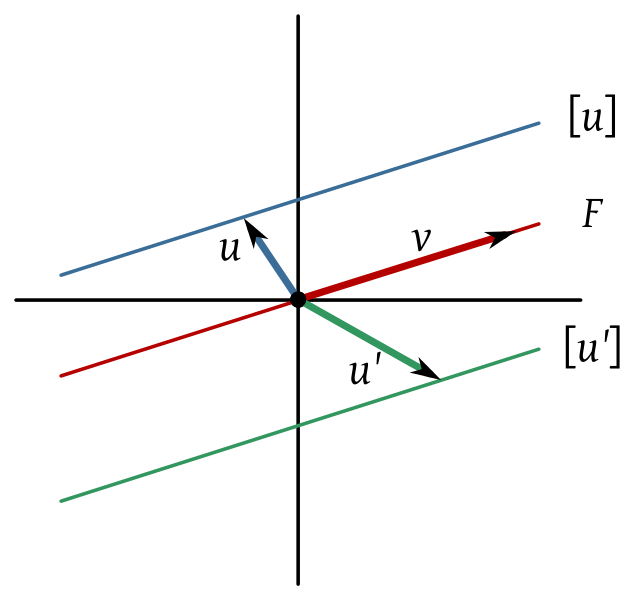
\includegraphics[scale=0.25]{clase lateral}
\end{center}

\subsubsection*{Conjunto Cociente}
Si definimos ahora: $\{[v]_W: v\in V\}=V/W$ al conjunto de clases laterales que se creen de $W$ se le conoce como \textbf{conjunto cociente} y forma un K-ESPACIO-VECTORIAL las siguientes propiedades:
\begin{itemize}
\item $\bar{v}+\bar{v'}=\overline{v+v'}$
\item $a\cdot \bar{v}=\overline{a\cdot v}$
\end{itemize}
Es notable destacar que $0_{V/W}=0_{\bar{v}}$ y que $-\bar{v}=\overline{-v}$. Comprobamos que la suma y el producto están bien definidos, para ver que $(W, +, \cdot )$ es un espacio vectorial:
$$\overline{v}_1=\overline{v}_2 \mbox{ represt. de una clase }\wedge \overline{v'}_1=\overline{v'}_2 \mbox{ de otra distinta}\Rightarrow$$
$$\overline{v_1+v_1'}=\overline{v_2+v_2'}\Leftrightarrow (v_1+v_1')-(v_2+v_2')=0\Leftrightarrow \underbrace{(v_1-v_2)}_{\in W}+\underbrace{(v_1'+v_2')}_{\in W}\in W$$
El producto se demuestra de forma análoga.

\subsubsection*{Proposición}
Si $\dim V=n$ y $\dim W=m\Rightarrow \dim V/W=n-m$.

\underline{Demostración}:\par
Elegimos una base cualquiera de $W$: $B_W=\{w_1,\cdots,w_m\}$ y ampliamos esta base para V: $B=\{w_1,\cdots, w_m, v_{m+1}, \cdots, v_n\}$, es decir, hemos añadido $n-m$ vectores a la base de $B_W$ para ampliarla a $B$. Ahora probamos que $\{\overline{v}_{m+1},\cdots \overline{v}_n\}$ es base de $V/W$.

\begin{itemize}
\item Linealmente independiente:
$$a_{m+1}\overline{v}_{m+1}+\cdots +a_n\overline{v}_n=0\Leftrightarrow \overline{a_{m+1}v_{m+1}+\cdots +a_nv_n}=0\Leftrightarrow a_{m+1}v_{m+1}+\cdots +a_nv_n- 0\in W$$
Como estos vectores pertenecen a $W$, entonces se podrán expresar en función de su base:
$$a_{m+1}v_{m+1}+\cdots +a_nv_n=a_1w_1+\cdots a_mw_m\Rightarrow a_{m+1}v_{m+1}+\cdots +a_nv_n-a_1w_1+\cdots a_mw_m=0\stackrel{B\mbox{ es base}}{\Rightarrow}\mbox{ l. ind.}$$

\item Sistema de generadores:
$$\forall v\in V: \overline{v}=\overline{a_1w_1+\cdots+a_mw_m+a_{m+1}v_{m+1}+\cdots+ a_nv_n}=\overline{a_1w_1+\cdots a_mw_m}+a_{m+1}\overline{v}_{m+1}+\cdots a_n\overline{v}_n=$$
Como $a_1w_1+\cdots a_mw_m\in W\Rightarrow \overline{a_1w_1+\cdots a_mw_m}=0$, luego tenemos que:
$$=a_{m+1}\overline{v}_{m+1}+\cdots a_n\overline{v}_n$$
Luego queda demostrado que para cualquier $\bar{v}$, este se puede expresar como combinación lineal de los vectores añadidos para ampliar la base, luego es sistema de generadores.

\end{itemize}

Ej.: En $\mathbb R^5$ consideramos $W$ como el subespacio de los vectores cuyas coordenadas se ajustan al siguiente sistema: $W=\begin{cases}
x_1+x_2-x_5=0 \\
2x_1-x_4=0
\end{cases}$, vamos a ver que $\dim W=3$ y vamos a calcular la base de $B_{V/W}$:\par
Podemos ver que el sistema de ecuaciones forma un subespacio vectorial de V por ser un sistema homgéneo del que son vectores los vectores solución de ese sistema. Su dimensión es el número de incógnitas menos el rango de la matriz de coeficientes, es decir, $\dim W=5-2=3$. Esto es así porque según vimos en Bachillerato, es necesario que haya 3 incógnitas parametrizadas que en este caso van a ser $x_3, x_4, x_5$ y las otras toman valores conforme a ellas, así que esencialmente los vectores de $W$ dependen de 3 valores, de ahí la dimensión 3.

Para hallar los vectores de la base de $W$, vemos que la solución del sistema es: $(x_1,x_2,x_3,x_4,x_5)=(\frac{x_4}{2}, x_5-\frac{x_4}{2},x_3,x_4,x_5)$. Por lo que cualquier vector solución se puede escribir como:
$$x_3(0,0,1,0,0)+x_4(1,-1,0,1,0)+x_5(0,1,0,0,1)$$
Otra forma es dar valores de vectores que sean linealmente independientes entre los tres parámetros, p. ej., $(x_3,x_4,x_5)=(1,0,0),(0,1,0), (0,0,1)$ y hallar los valores de $x_1$ y $x_2$ para completar con las dos variables que faltan cada uno de los vectores.\par
Con lo cual, para encontrar la base ahora de $V/W$, vemos que  vectores es necesario añadir a la hallada para que sea base de $V$, un caso sencillo para ampliar la base es añadir vectores de la base canónica de $\mathbb R^5$:
$$B=\{(0,0,1,0,0),(1,-1,0,1,0),(0,1,0,0,1), v_1, v_2\}=$$
$$=\{(0,0,1,0,0),(1,-1,0,1,0),(0,1,0,0,1), e_1=(1,0,0,0,0), e_2=(0,1,0,0,0)\}$$
Con lo cual, $e_1$ y $e_2$ forman la base de $V/W$.

\section*{APLICACIONES LINEALES}
Por definición, una aplicación $\phi:V\longrightarrow V'$ es una aplicación lineal entre dos espacios vectoriales si conserva la suma y el producto por un escalar\footnote{Nótese que no aparece la condición de biyectividad de los isomorfismos}:
$$\phi(v_1+v_2)=\phi(v_1)+\phi(v_2): \forall v_1,v_2\in V$$
$$\phi(a\cdot v_1)=a\cdot \phi(v_1): \forall a\in K,\forall v\in V$$
Por notación vamos a referirnos al conjunto de las aplicaciones lineales de V a V' como $Hom(V,V')$, cuando vemos que la aplicación lineal va de V a V, entonces lo llamamos $End(V,V)$

Ej.: $\phi: K^3\longrightarrow K^2$ y $\phi(x,y,z)=(x-y, x+y+z)$:
$$\phi\left[(x,y,z)+(x',y',z')\right]=\phi(x+x',y+y',z+z')=(x+x'-y-y', x+x'+y+y'+z+z')=$$
$$=(x-y, x+y+z)+(x'+y',x'+y'+z')=\phi(x,y,z)+\phi(x',y',z')$$

Ej.: $\phi: V\longrightarrow V$ y sea $\phi$ $K-lineal$, entonces decimos que es un endomorfismo. Por ejemplo, $\phi: V\longrightarrow V$ siendo $id_V=\phi(v)=v$, es un endomorfismo.

Ej.: $\phi: V\longrightarrow V$ y sea $\phi(v)=r\cdot v$ donde $r\in K$, también es un isomorfismo. Concretamente a esto se le conoce como \textbf{homotecia}\footnote{Y en este caso además es un isomorfismo dentro del propio V}. $\phi$ cumple que $\phi=\phi^{-1}$ con lo que es fácil demostrar que es una biyección y por extensión un isomorfismo. 

Ej.: Si tenemos $W<V$, podemos definir $V/W$ y ahora $\phi: V\longrightarrow V/W$ siendo $\phi(v)=\bar{v}$, entonces $\phi$ es aplicación lineal.

Ej.: Si tenemos que $V=W\oplus U$ y $\phi: V\longrightarrow V$, entonces $v=w+u$ de modo único y la aplicación $\phi(v)=w$ es lineal. A esta aplicación se la conoce como \textbf{proyección} de $v$ con base $W$ y dirección $U$.
\begin{itemize}
\item Vamos a ver que ocurre con los vectores de $W$:
$$v\in W\Leftrightarrow \phi(v)=v$$

Esto es así porque:
$$v\in W\Rightarrow v=\underbrace{v}_{\in W}+\underbrace{0}_{\in U}\Rightarrow \phi(v)=v$$
$$\phi(v)=v\Rightarrow v=\underbrace{w}_{=v}+u\Rightarrow u=0\Rightarrow v\in W$$

\item Vamos a ver que ocurre con los vectores de $U$:
$$v\in U\Leftrightarrow \phi(v)=0$$

Esto es así porque:
$$v\in U\Rightarrow v=\underbrace{0}_{\in W}+\underbrace{v}_{\in U}\Rightarrow \phi(v)=0$$
$$\phi(v)=0\Rightarrow v=\underbrace{w}_{=0}+u\in U$$
\end{itemize}

Ej.: Si tenemos que $V=W\oplus U$, entonces $v=w+u$ de modo único y la aplicación $\phi(v)=w-u$ es lineal. A esta aplicación se la conoce como \textbf{simetría} de $v$ con base $W$ y dirección $U$.
\begin{itemize}
\item Vamos a ver que ocurre con los vectores de $W$:
$$v\in W\Leftrightarrow \phi(v)=v$$

Esto es así porque:
$$v\in W\Rightarrow v=\underbrace{v}_{\in W}+\underbrace{0}_{\in U}\Rightarrow \phi(v)=v-0=v$$
$$\phi(v)=v\Rightarrow w-u=v=\underbrace{w}_{=v}+u\Rightarrow 2u=0\Rightarrow v=w\in W$$

\item Vamos a ver que ocurre con los vectores de $U$:
$$v\in U\Leftrightarrow \phi(v)=-v=-1_k\cdot v$$

Esto es así porque:
$$v\in U\Rightarrow v=\underbrace{0}_{\in W}+\underbrace{v}_{\in U}\Rightarrow \phi(v)=0-v=-v$$
$$\phi(v)=-v\Rightarrow w-u=-v=-w-u\Rightarrow 2w=0\Rightarrow v=u\in U$$
\end{itemize}

\subsection*{\underline{Imagen y Núcleo}}
Si $\phi: V\longrightarrow V'$, decimos que la imagen de $\phi$ es el subespacio vectorial del espacio de llegada cuyos vectores son imagen de algún vector del espacio de salida:
$$Im(\phi)=\{\phi(v): v\in V\}<V'$$
Y conocemos como el núcleo de $\phi$ al subespacio vectorial del espacio inicial cuyos vectores se transforman en el vector nulo del espacio de llegada:
$$Ker(\phi)=\{v\in V: \phi(v)=0_v\}<V$$

\subsubsection*{Proposición}
Sea $\phi: V\longrightarrow V'$, decimos que:
\begin{enumerate}
\item $\phi$ es suprayectiva $\Leftrightarrow Im(\phi)=V'$
\item $\phi$ es inyectiva $\Leftrightarrow Ker(\phi)=\{0_v\}$
\end{enumerate}

\underline{Demostración}:
\begin{enumerate}
\item trivial

\item De la primera se deduce que:
\begin{itemize}
\item ``$\Rightarrow$'': supongamos que es inyectiva\par
Vemos primero que: $\phi(0_v)=\phi(0_v+0_v)=\phi(0_v)+\phi(0_v)\Leftrightarrow 0_v'=\phi(0_v)\Rightarrow 0_v\in Ker(\phi)$.
$$v\in Ker(\phi)\Rightarrow \phi(v)=0_v'\Rightarrow \phi(v)\phi(0)\Rightarrow v=0:\forall v\in Ker(\phi)$$

\item ``$\Leftarrow$'': supongamos cierto que el $Ker(\phi)=\{0_v\}$.
$$\phi(v_1)=\phi(v_2)\Rightarrow \phi(v_1-v_2)=0_v'\Rightarrow v_1-v_2\in Ker(\phi)\Rightarrow v_1-v_2=0_v\Rightarrow v_1=v_2$$
\end{itemize}
\end{enumerate}

\textbf{Proyecciones}\par

Para las proyecciones resulta que la base es la imagen y la dirección es el núcleo de la misma, es decir, $Im(\phi)=W$ y $Ker(\phi)=U$, siendo $V=W\oplus U$. Además, en las proyecciones $\phi^2=\phi$.\par

\underline{Demostración}:
\begin{itemize}
\item $W=Im(\phi)$
\begin{itemize}

\item ``$\subset$'':
$$w\in W\Rightarrow w=w+0\Rightarrow \phi(w)=w\Rightarrow w\in Im(\phi)$$

\item ``$\supset$'':
$$w\in Im(\phi)\Rightarrow w=\phi(v)\Rightarrow \phi(v)\in W$$
\end{itemize}

\item $U=Ker(\phi)$:
$$v\in U\Leftrightarrow \phi(v)=0\Rightarrow v\in Ker(\phi)$$

\item $\phi \mbox{ proyección}\Leftrightarrow \phi^2=\phi$
\begin{itemize}
\item ``$\Rightarrow$'':
$$\phi^2(v)=\phi^2(w+u)=\phi(\phi(w+u))=\phi(w)=w=\phi(v)$$
Por ello se las llama idempotencias.

\item ``$\Leftarrow$'': tenemos que ser capaces de componer, sabiendo que $\phi^2=\phi$, que $V=W\oplus V$ siendo $W=\{v\in V: \phi(v)=v\}$ base de la simetría y $U=\{v\in V: \phi(v)=0\}$ dirección de la simetría. Es decir, partimos de la hipótesis y de la definición de ambos subespacios y hay que demostrar la suma directa.
$$v\in W\cap U\Leftrightarrow 0=\phi(v)=v\Leftrightarrow v=0\Rightarrow W\cap U=\{0\}$$
$$\phi(v)\in W\wedge v-\phi(v)\in U\Rightarrow v=\phi(v)+v-\phi(v)$$

Esto es así porque $\phi(\phi(v))=\phi^{2}(v)=\phi(v)\Rightarrow \in W$ y $\phi(v-\phi(v))=\phi(v)-\phi^2(v)=0\Rightarrow \in U$.

Solo falta ver que existe una proyección de $V$ con base $W$ y dirección $U$ que como es única, esta debe coincidir necesariamente con $\phi$:
$$\varphi: V\longrightarrow V\mbox{ proyección con base W y dirección U}\Rightarrow W=\{v\in V: \varphi(v)=v\}\wedge U=\{v\in V: \varphi(v)=0\}\Rightarrow$$
$$\Rightarrow v\in W \vee v\in U: \phi(v)=\varphi(v)\Rightarrow v\in V: v=w+u\Rightarrow \phi(v)=\phi(w)+\phi(u)=\varphi(w)+\varphi(u)=\varphi(v):\forall v\in V$$
\end{itemize}
\end{itemize}

Además, $\phi$ es suprayectiva:
$$\Leftrightarrow Im(\phi)=V\Leftrightarrow W=V \wedge U=\{0\}\Leftrightarrow id_v=\phi$$

Además, $\phi$ es inyectiva:
$$\Leftrightarrow Ker(\phi)=\{0\}\Leftrightarrow V=\{0\}\Leftrightarrow W=V\Leftrightarrow \phi=id_v$$

\textbf{Simetrías}\par

Para las simetrías resulta que $Im(\phi)=V$ y $Ker(\phi)=\{0\}$, por lo tanto todas las simetrías son inyectivas y suprayectivas y en consecuencia, isomorfismos. Además, en las simetrías $\phi=\phi^{-1}$.\par

\underline{Demostración}:
\begin{itemize}
\item $V=Im(\phi)$
$$v\in V\Leftrightarrow v=w+u \Rightarrow w-(-u)=\phi(w-u)\in Im(\phi)$$

\item $\{0\}=Ker(\phi)$:
$$v\in Ker(\phi)\wedge v=w+u\Rightarrow w+u=v=0=\phi(v)=w-u\Rightarrow u=w\Rightarrow u=w\in U\cap W=\{0\}\Rightarrow u=w=0=v$$

\item $\phi \mbox{ simetría}\Leftrightarrow \phi^{-1}=\phi$
\begin{itemize}
\item ``$\Rightarrow$'':
$$(\phi \circ \phi)(v)=\phi(\phi (v))=\phi(w-u)=w-(-u)=w+u=v\Rightarrow \phi=id_v$$
Por ello se las llama involuciones

\item ``$\Leftarrow$'': tenemos que ser capaces de componer, sabiendo que $\phi^2=id_V$, que $V=W\oplus V$ siendo $W=\{v\in V: \phi(v)=v\}$ base de la simetría y $U=\{v\in V: \phi(v)=-v\}$ dirección de la simetría. Es decir, partimos de la hipótesis y de la definición de ambos subespacios y hay que demostrar la suma directa.
$$v\in W\cap U\Leftrightarrow -v=\phi(v)=v\Leftrightarrow v=0\Rightarrow W\cap U=\{0\}$$
$$v+\phi(v)\in W\wedge v-\phi(v)\in U\Rightarrow v=\frac{v+\phi(v)}{2}+\frac{v-\phi(v)}{2}$$

Esto es así porque $\phi(v+\phi(v))=\phi(v)+v\Rightarrow \in W$ y $\phi(v-\phi(v))=\phi(v)-v\Rightarrow \in U$.

Solo falta ver que existe una simetría de $V$ con base $W$ y dirección $U$ que como es única, esta debe coincidir necesariamente con $\phi$:
$$\varphi: V\longrightarrow V\mbox{ simetría con base W y dirección U}\Rightarrow W=\{v\in V: \varphi(v)=v\}\wedge U=\{v\in V: \varphi(v)=-v\}\Rightarrow$$
$$\Rightarrow v\in W \vee v\in U: \phi(v)=\varphi(v)\Rightarrow v\in V: v=w+u\Rightarrow \phi(v)=\phi(w)+\phi(u)=\varphi(w)+\varphi(u)=\varphi(v):\forall v\in V$$
\end{itemize}
Por último, la relación que existe, dada la misma base y la misma dirección, entre las simetrías y las proyecciones es: $\mbox{Sean }\phi\mbox{ simetría y }\varphi \mbox{ la proyección asociada}$:
$$\begin{cases}\phi(v)=w-u \\ \varphi(v)=w \\ id(v)=w+u\end{cases}\Rightarrow (\phi+id)(v)=2w=2\varphi(v)\Rightarrow \frac{1}{2}\cdot (\phi + id)=\varphi$$
\end{itemize}

\subsection*{\underline{Operaciones con aplicaciones lineales}}
Supongamos que tenemos: $\phi_1, \phi_2: V\longrightarrow V'$ siendo ambas $K-lineales$, entonces:
\begin{itemize}
\item $(\phi_1+\phi_2)(v)\stackrel{Def}{=}\phi_1(v)+\phi_2(v):\forall v\in V$
\item $(a\cdot \phi_1)(v)\stackrel{Def}{=}a\cdot \phi_1(v):\forall v\in V$
\end{itemize}

Entonces podemos considerar $(Hom(V,V'),+,\cdot )$ como un espacio vectorial.\par

Del mismo modo se puede ver que $(\phi_2 \circ \phi_1)(v)$ es también una aplicación lineal si ambas aplicaciones lo son. Con lo que $(End(V), +, \circ)$ es un anillo conmutativo y unitario.

\subsection*{\underline{Teorema}}
Supongamos $V$ y $V'$ espacios vectoriales y $\{v_1, ..., v_n\}$ base de $V$ y $v_1', ..., v_n'\in V'$ vectores arbitrarios de $V'$ el teorema dice que:
$$\exists! \phi: V\longrightarrow V': \phi(v_i)=v_i': \forall i=1,...,n$$

Esto quiere decir que una aplicación lineal entre dos espacios vectoriales está determinada de modo único por la imagen de los vectores de la base del espacio de partida.

\underline{Demostración}:
\begin{itemize}
\item Existencia:
Sea $v\in V: v=(a_1, ..., a_n)_B$ quiere decir que $v=\sum_{i=1}^n a_iv_i$. Ahora definimos $\phi(v)=\sum_{i=1}^na_iv_i'$ y vemos que es lineal:
$$w=(b_1,...,b_n)_B\Rightarrow v+w=(a_1+b_1,..., a_n+b_n)_b\Rightarrow \phi(v+w)=\sum_{i=1}^n (a_i+b_i)v_i'=\sum_{i=1}^na_iv_i' + \sum_{i=1}^nb_iv_i'=\phi(v)+\phi(w)$$
$$a\cdot v=(a\cdot a_1, ..., a\cdot a_n)_B\Rightarrow \phi(a\cdot v)=\sum_{i=1}^n(a\cdot a_i)v_i'=a\cdot \sum_{i=1}^na_iv_i'=a\cdot \phi(v)$$

Y ahora vemos que se demuestra la existencia:
$$v_i=(0,...,1,...,0)_B\Rightarrow \phi(v_i)=1\cdot v_i'=v_i'$$

\item Unicidad:
$$\mbox{Suponemos que hay dos y vemos que van a cumplir: }\phi(v_i)=\varphi(v_i)=v_i': \forall i=1,...,n$$
$$\phi(v)=\phi(\sum_{i=1}^na_iv_i)=\sum_{i=1}^na_i\phi(v_i)=\sum_{i=1}^na_iv_i'$$
$$\varphi(v)=\varphi(\sum_{i=1}^na_iv_i)=\sum_{i=1}^na_i\varphi(v_i)=\sum_{i=1}^na_iv_i'$$
\end{itemize}

Esto lo que quiere decir es que si suponemos que $V=K^2$ y $V'=K^3$ entonces solo hay una aplicación lineal que cumpla que $\phi(e_1)=(2,1,-3)$ y $\phi(e_2)=(0,1,0)$, con lo cual sabiendo la relación que existe entre los vectores de la base de un espacio y los vectores del espacio de llegada podemos definir de modo único la aplicación que las relaciona.
$$\phi(a_1, a_2)=\phi(a_1e_1+a_2e_2)=a_1(2,1,-3)+a_2(0,1,0)=(2a_1, a_1+a_2, -3a_1)$$

\subsection*{\underline{Teorema}}
Dos espacios vectoriales son isomorfos si y solo si la dimensión de ambos es la misma.
$$V\simeq V'\Leftrightarrow \dim_k V=\dim_k V'$$

\underline{Demostración}:
\begin{itemize}
\item ``$\Rightarrow$'': vamos a ver que $B'=\{\phi(v_1), ..., \phi(v_n)\}$ es base de V'\par
Sea $B=\{v_1, ..., v_n\}$ base de $V$ y $\phi: V\longrightarrow V'$ un isomorfismo, entonces:
$$v'\in V\stackrel{isomf}{\Rightarrow} v'=\phi(v)=\phi(a_1v_1+...+a_nv_n)=a_1\phi(v_1)+...+a_n\phi(v_n)\Rightarrow \{\phi(v_1), ..., \phi(v_n)\}\mbox{ es sist. gener.}$$
Ahora vemos que son linealmente independientes:
$$0=a_1\phi(v_1)+...+a_n\phi(v_n)=\phi(a_1v_1+...+a_nv_n)\Rightarrow a_1v_1+...+a_nv_n\in Ker(\phi)=\{0\}\Rightarrow 0=a_1v_1+...+a_nv_n=0$$

\item ``$\Leftarrow$'':\par
Sea $B=\{v_1, ..., v_n\}$ base de $V$ y $B'=\{v_1', ..., v_n'\}$ base de $V'$, entonces:
$$\exists! \phi: V\longrightarrow V': \phi(v_i)=v_i': \forall i=1,..., n$$
$$\exists! \varphi: V'\longrightarrow V: \varphi(v_i')=v_i: \forall i=1,..., n$$

$$\varphi \circ \phi: V\longrightarrow V\Rightarrow (\varphi \circ \phi)(v_i)=\varphi(v_i')=v_i\Rightarrow \varphi \circ \phi=id_V$$
Pero del mismo modo se sigue que:
$$\phi \circ \varphi: V\longrightarrow V\Rightarrow (\phi \circ \varphi)(v_i)=\phi(v_i')=v_i\Rightarrow \phi \circ \varphi=id_{V'}$$

Lo que implica que ambas son biyectivas y como son lineales, ambas son isomorfismos.
\end{itemize}

\subsection*{\underline{Teorema}}
Si la dimensión de un espacio cualquiera es $n$, entonces es isomorfo al producto cartesiano de $n$ veces $K$.
$$\dim_k V=n\Rightarrow V\simeq K^n$$

\underline{Demostración}:\par
$$\dim_k V=n=\dim_k K^n\Rightarrow V\simeq K^n$$

Sin embargo no podemos decir que exista un isomorfismo canónico que verifique este teorema, solo podemos afirmar que existe porque para poder afirmarlo es necesario definir una base de $V'$ y cambia en función de la base elegida.

\subsection*{\underline{Teorema de la dimensión}}
Supongamos que $\phi: V\longrightarrow V'$ es lineal y que $\dim_k V=n$, entonces se cumple que:
\begin{enumerate}
\item $Ker(\phi)$ y $Im(\phi)$ son de dimensión finita
\item $\dim_k Ker(\phi)+\dim_k Im(\phi)=n$
\end{enumerate}

\underline{Demostración}:
\begin{enumerate}
\item $\begin{cases} Ker(\phi)>V\\ \dim_k V=n\end{cases}\Rightarrow \dim_k Ker(\phi)\leq n$, por tanto elijo una base de V: $B=\{v_1,..., v_r, \underbrace{v_{r+1}, ..., v_n}_{B\mbox{ de }Ker(\phi)}\}$. Es decir, escogemos una base del $Ker(\phi)$ que posee $n-r$ vectores y después por el \textbf{teorema de la extensión de la base}, construimos una base de V.\par

Vamos a ver que $\{\phi(v_1), ..., \phi(v_r)\}$ es una base de la $Im(\phi)$:
$$v'\in Im(\phi)\Rightarrow v'=\phi(v)=\phi(a_1v_1+...+a_rv_r+a_{r+1}v_{r+1}+...+a_nv_n)=$$
$$=a_1\phi(v_1)+...+a_r\phi(v_r)+a_{r+1}v_{r+1}+...+a_n\phi(v_n)=a_1\phi(v_1)+...+a_r\phi(v_r)$$

Y ahora vemos que estos son linealmente independientes:
$$0=a_1\phi(v_1)+...+a_r\phi(v_r)=\phi(a_1v_1+...+a_rv_r)\Rightarrow a_1v_1+...+a_rv_r\in Ker(\phi)\Rightarrow a_1v_1+...+a_rv_r=$$
$$=a_{r+1}v_{r+1}+...+a_nv_n\Leftrightarrow a_1v_1+...+a_rv_r-a_{r+1}v_{r+1}-...-a_nv_n=0\Rightarrow a_1=...=a_r=a_{r+1}=...=a_n=0$$
\end{enumerate}

\subsubsection*{Primer Teorema de Isomorfía}
Supongamos que $\phi: V\longrightarrow V'$ es una aplicación K-lineal se cumple que:
$$V/Ker(\phi)\simeq Im(\phi)$$
Este teorema vale siempre, sea cual sea la dimensión de V

\underline{Demostración}:\par
Supongamos que $V$ es de dimensión finita, entonces $Ker(\phi)$ y $Im(\phi)$ también son finitos por el teorema de la dimensión, además sabemos que:
$$\dim V= \dim Ker(\phi)+ \dim Im(\phi)\Leftrightarrow \dim V- \dim Ker(\phi)=\dim Im(\phi)\Leftrightarrow \dim V/Ker(\phi)=\dim Im(\phi)$$
$$\Rightarrow V/Ker(\phi)\simeq Im(\phi)$$

Vamos ahora a ver la aplicación lineal que relaciona ambos conjuntos y establece el isomorfismo:
$$\bar{\phi}: V/Ker(\phi) \longrightarrow Im(\phi)$$
$$\overline{\phi}(\bar{v})=\phi(v)$$

De este modo ya se cumple el isomorfismo, pero hay que comprobar que está bien definida probando que:
$$\bar{v}=\bar{w}\Rightarrow \phi(v)=\phi(w)$$

Y por último también que:
$$\phi \mbox{ es lineal, inyectiva y suprayectiva}$$

\subsubsection*{Segundo Teorema de Isomorfía}
Consideramos $W, U<V$ y definimos los subespacios:
$$(W+U)/W\simeq U/(W\cap U)$$

\underline{Demostración}:\par
Considerando $W$ y $U$ de dimensión finita, entonces $W+U$ es de dimensión finita y $W\cap U$ también lo es. Ahora vemos que:
$$\dim (W+U/W)=\dim (W+U)- \dim W\stackrel{Grassman}{=}\dim U-\dim (W\cap U)=\dim (U/W\cap U)$$

\subsection*{\underline{Teorema de la Matriz Asociada}}
Suponemos que $\phi: V\longrightarrow V'$ una aplicación K-lineal, $B=\{v_1,..., v_n\}$ base de $V$ y $B'=\{v_1',..., v_m'\}$ base de $V'$.\par

Por uno de los teoremas anteriores, $\phi$ está determinado de modo único por su valor en los vectores de la base $B$.
$$\begin{cases}\phi(v_1)=a_{11}v_1'+...+a_{m1}v_m'
\\ \vdots \\ \phi(v_n)=a_{1n}v_1'+...+a_{mn}v_m'\end{cases}$$

Con lo cual, podemos construir una matriz:
$$M_{B,B'}(\phi)=\underbrace{\left(\begin{array}{ccc} \overbrace{a_{11}}^{\phi(v_1)} & \cdots & \overbrace{a_{1n}}^{\phi(v_n)} \\ \vdots & \ddots & \vdots \\ a_{m1} & \cdots & a_{mn} \end{array}\right)}_{\mbox{En base }B'}\in Mat_{m\times n}(K)$$

Por lo tanto, ¿cómo podemos recuperar la aplicación $\phi$ a partir de su matriz asociada en términos de $B$ y $B'$? Expresamos un vector genérico de $V$ en términos de la base B:
$$\phi(x_1v_1+...+x_nv_n)=x_1\phi(v_1)+...+x_n\phi(v_n)=x_1(a_{11}v_1'+...+a_{m1}v_m')+... + x_n(a_{1n}v_1'+...+a_{mn}v_m')=$$
$$=\underbrace{(a_{11}x_1+...+a_{1n}x_n)}_{x_1'}v_1'+...\underbrace{(a_{m1}x_1+...+a_{mn}x_n)}_{x_m'}v_m'\Rightarrow$$
$$\Rightarrow \phi(v)=\phi(x_1v_1+...+x_nv_n)=(a_{11}x_1+...+a_{1n}x_n)v_1'+...(a_{m1}x_1+...+a_{mn}x_n)v_m'=x_1'v_1'+...+x_m'v_m'=v'$$

Con lo cual para transformar un vector en otro tenemos que:
$$\left(\begin{array}{c} \overbrace{x_1'}^{\phi(v)} \\ \vdots\\ x_m'\end{array}\right)=\left(\begin{array}{ccc} \overbrace{a_{11}}^{\phi(v_1)} & \cdots & \overbrace{a_{1n}}^{\phi(v_n)} \\ \vdots & \ddots & \vdots \\ a_{m1} & \cdots & a_{mn} \end{array}\right)\cdot \left(\begin{array}{c} \overbrace{x_1}^{v} \\ \vdots\\ x_n\end{array}\right)$$

Ej.: Consideremos $\phi: \mathbb R^2 \longrightarrow \mathbb R^2$ y que $\phi(e_1)=\frac{3e_1+4e_2}{5}$ y $\phi(e_2)=\frac{4e_1-3e_2}{5}$, entonces tenemos que:
$$A=M_{B_c}(\phi)=\left(\begin{array}{cc} \frac{3}{5} & \frac{4}{5} \\ \frac{4}{5} & \frac{-3}{5}\end{array}\right)\Rightarrow A^2=I \Rightarrow \phi^2=id_{\mathbb R^2}\Rightarrow \mbox{ simetría}$$

Con lo cual, $\phi$ posee base $W$ y dirección $U$ de la simetría, entonces:
$$v=(x_1,x_2)_B\in W\Leftrightarrow \phi(v)=v\Leftrightarrow \begin{pmatrix}
x_1 \\
x_2
\end{pmatrix}=A\begin{pmatrix}
x_1\\
x_2
\end{pmatrix}\Leftrightarrow W: x_1-2x_2=0
$$

Para hallar el subespacio $U$ el procedimiento es el mismo.

\subsubsection*{Propiedades}
\begin{itemize}
\item Supongamos $V\stackrel{\phi_1, \phi_2}{\longrightarrow} V'$ y $B$ y $B'$ bases respectivas, entonces:
$$M_{B,B'}(\phi_1+\phi_2)=M_{B,B'}(\phi_1)+=M_{B,B'}(\phi_2)$$

\item Del mismo modo, si $a\in \mathbb K$ y $\phi: V\longrightarrow V'$, entonces:
$$M_{B,B'}(a\cdot \phi)=a \cdot M_{B,B'}(\phi)$$

\item Por último, $V\stackrel{\phi}{\longrightarrow} V'\stackrel{\varphi}{\longrightarrow } V''$, entonces:
$$M_{B,B''}(\varphi\circ \phi)=M_{B,B''}(\varphi)\cdot =M_{B,B''}(\phi)$$
\end{itemize}

Además, comentamos anteriormente que $(Hom_k(V,V'), +, \cdot )$ forma un espacio vectorial, por lo que podemos establecer tomando $\dim V=n$ y $\dim V'=m$:
\begin{eqnarray*} \Phi:(V,V') &\longrightarrow& Mat_{m\times n}(K)\\ \phi &\longmapsto& M_{B,B'}(\phi) 
\end{eqnarray*} 

Y esta aplicación es un isomorfismo de espacios vectoriale:
$$Hom_k(V,V')\simeq Mat_{m\times n}(K)$$

\underline{Demostración}:
\begin{itemize}
\item Está bien definida porque ya comprobamos que toda aplicación lineal está definida de módo único por la transformación de los vectores de una base y además cada aplicación podía escribirse en forma de matriz, que está asociada a cada $\phi$.

\item La suma y el producto se respetan de forma trivial.

\item Que es inyectiva:
$$\phi\in Ker(\phi)\Rightarrow \Phi(\phi)=0\Rightarrow \Phi(\phi)=Mat_{B,B'}(\phi)\Rightarrow \phi(v_1)=...=\phi(v_n)=0\Rightarrow \phi=0\Rightarrow Inyectiva$$

\item Ahora que es suprayectiva:
$$A=\begin{pmatrix}
a_{11} & \cdots & a_{1n} \\ \vdots & \ddots & \vdots \\ a_{m1} & \cdots & a_{mn}\end{pmatrix}\in Mat_{m\times n}(K)\Rightarrow \exists \phi: V\longrightarrow V'\mbox{ tal que }\phi(v_i)=a_{1i}v_1'+...+a_{mi}v_m'\Rightarrow \exists!\phi\Rightarrow Sobre$$

Como para que la imagen de $\phi$ sea $A$ tiene que definirse a partir de los vectores de V', entonces es única porque ya demostramos que estos la determinan.
\end{itemize}

Análogamente, si consideramos $(End_k(V), +, \circ)$ que forma un anillo unitario, entonces $End_k(V)\simeq Mat_n(K)$:
\begin{eqnarray*} \Phi:(V,V) &\longrightarrow& Mat_{m\times n}(K)\\ \phi &\longmapsto& M_{B}(\phi) 
\end{eqnarray*} 


\subsection*{\underline{Relación entre matrices asociadas de la misma aplicación}}
Sea $A_1, A_2\in Mat_{m\times n}(K)$, $V, V'$ espacios vectoriales cuyas dimensiones son $\dim V=n$ y $\dim V'=m$, son equivalentes:
$$A_1\thicksim A_2 \Leftrightarrow \exists \phi: V\longrightarrow V'\mbox{ lineal y bases } B_1,B_2\mbox{ de }V \mbox{ y bases }B_1', B_2'\mbox{ de }V': A_1=M_{B_1,B_1'}(\phi) \wedge A_2=M_{B_2,B_2'}(\phi)$$

Para entender este concepto vamos a ver con cuidado todo el desarrollo del razonamiento teórico:\par

Sea $\phi: V\longrightarrow V'$ y $B_1, B_2$ bases de $V$ y $B_1', B_2'$ bases de $V'$, definimos las matrices:

$$\begin{cases}A_1=Mat_{B_1,B_1'}(\phi)\\ A_2=Mat_{B_2,B_2'}{}(\phi)\end{cases}$$

\begin{center}
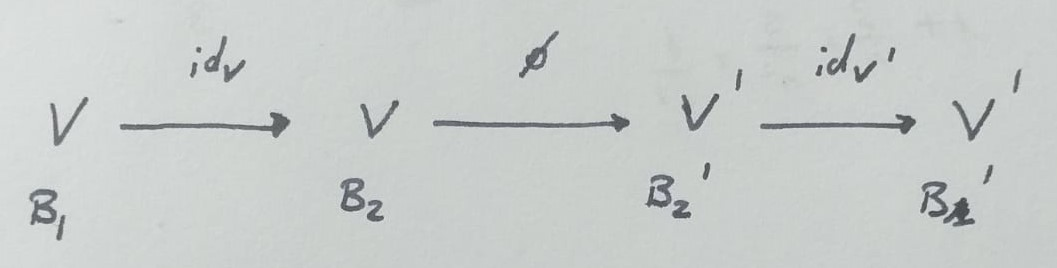
\includegraphics[scale=0.35]{Matrices equivalentes}
\end{center}
$$A_1=M_{B_1,B_1'}(\phi)=M_{B_2',B_1'}(id_{V'})\cdot M_{B_2,B_2'}(\phi)\cdot M_{B_1, B_2}(id_V)=\underbrace{M(B_2',B_1')}_{Q}\cdot A_2\cdot \underbrace{M(B_1,B_2)}_{P}=Q\cdot A_2\cdot P$$

Sabemos, por ser matrices de paso, que $Q\in Mat_m(K)^x=Gl_m(K)$ y $P\in Mat_n(K)^x=Gl_n(K)$, es decir, existen sus inversas.

Por lo tanto, sean $A_1$ y $A_2$ matrices $m\times n$ en K, se dice que esas matrices son equivalentes si $A_1=Q\cdot A_2\cdot P$ donde $Q$ y $P$ son inversibles de los tamaños adecuados.
$$A_1\approx A_2 \Leftrightarrow A_1=Q\cdot A_2\cdot P$$

Esto quiere decir que para una misma aplicación lineal existen varias representaciones matriciales en función de la base escogida que la defina, pero sin embargo, por medio de esta fórmula se relacionan todas las que representan la misma  aplicación. Vemos, por tanto, que esta relación establece una relación de equivalencia entre las matrices que representan a la misma $\phi$, es decir, todas las matrices que representan a la misma $\phi$ son equivalentes y pertenecen a la misma clase de equivalencia.

\subsubsection*{Proposición}
Sea $P\in Gl_n(K)$, sea $V$ de dimensión $n$ y $B$ base de $V$. Si $P=\begin{pmatrix} p_{11} & \cdots & p_{1n} \\ \vdots & \ddots & \vdots \\ p_{m1} & \cdots & p_{mn}\end{pmatrix}$ y $B'=\{\phi(v_1), ..., \phi(v_n)\}$, siendo $v_i$ los vectores de $B$, entonces:
\begin{enumerate}
\item $B'=\{v_1'=\sum_{i=1}^np_{i1}v_i, ..., v_n'=\sum_{i=1}^n p_{in}v_i\}$ es base de V.\par
Es decir, la suma del producto de cada elemento de la columna $i$-ésima de la matriz $P$, por el vector $i$-ésimo de la base $B$, es un vector que forma otra base de $V$.

\item $P=M(B',B)$
\end{enumerate}

Esto nos lleva a considerar que TODA matriz inversible se puede considerar como una matriz de cambio de base dentro de un espacio vectorial.

\underline{Demostración}:
\begin{enumerate}
\item Supongamos:
$$0=a_1v_1'+\cdots+ a_nv_n'=a_1(p_{11}v_1+\cdots p_{n1}v_n)+\cdots +a_n(p_{1n}v_1+\cdots p_{nm}v_n)=$$
$$=(p_{11}a_1+\cdots p_{1n}a_n)v_1+\cdots +(p_{n1}a_1+\cdots +p_{nm}a_n)v_n\Rightarrow $$

Como los vectores $v_i$ formaban una base por hipótesis, tenemos que:
$$\Rightarrow 
\begin{cases}
p_{11}a_1+\cdots p_{1n}a_n=0 \\
\vdots \\
p_{n1}a_1+\cdots +p_{nm}a_n
\end{cases}\Rightarrow P\cdot \begin{pmatrix} a_1 \\ \vdots \\ a_n\end{pmatrix}= \begin{pmatrix} 0 \\ \vdots \\ 0\end{pmatrix}\Leftrightarrow   \begin{pmatrix} a_1 \\ \vdots \\ a_n\end{pmatrix}= P^{-1}\cdot \begin{pmatrix} 0 \\ \vdots \\ 0\end{pmatrix}=0\Rightarrow \forall i=0,..., n: a_i=0\Rightarrow $$
$$\Rightarrow \{v_1', ..., v_n'\}\mbox{ l. ind.}\stackrel{\dim V=n}{\Rightarrow} \{v_1', ..., v_n'\}\mbox{ es base}
$$

\item Probada la 1ª la segunda es inmediata porque si probamos lo primero, coger cada vector de $B'$ y lo expreso en base $B$, sus coordenadas son los coeficientes de la matriz $P$.
\end{enumerate}

\subsection*{\underline{Rango de una aplicación lineal}}
Sea $\phi: V\longrightarrow V'$ una aplicación lineal y $A\in Mat_{m\times n}(K)$ donde $A=\begin{pmatrix} a_{11} & \cdots  & a_{1n}\\ \vdots & \ddots & \vdots \\ a_{m1} & \cdots &a_{mn}\end{pmatrix}$ entonces:
\begin{enumerate}
\item $rg(\phi)=\dim_k Im(\phi)$
\item $rg(A)=\dim_k L(a_{11}e_{1}+...+a_{m1}e_m, ..., a_{1n}e_1+...+a_{mn}e_m)$.\par
Es decir, que $rg(A)$ es el subespacio generado por los vectores columnas de la matriz A (que están expresados en función de la base canónica de $K^m$.
\end{enumerate}

En dimensión finita, $\dim V=\dim Ker(\phi)+\dim Im(\phi)=\dim Ker(\phi)+ rg(\phi)$.

\subsubsection*{Lema}
Este teorema dice que para la condición 2) que se ha dado en la definición de rango de una aplicación lineal, se pueden utilizar los vectores de la base de un espacio de dimensión $m$ cualquiera, es decir, que no es necesario que sean los del espacio $K^m$ ni tampoco los de la base canónica de un espacio.

Supongamos que $A=(a_{ij})\in Mat_{m\times n}(K)$, entonces vamos a llamar $W$ a un espacio vectorial cualquiera cuya $\dim W=m$ y $B=\{w_1, ..., w_m\}$ base del mismo. Entonces se verifica que:
$$rg(A)=\dim L(a_{11}w_{1}+...+a_{m1}w_m, ..., a_{1n}w_1+...+a_{mn}w_m)$$

\underline{Demostración}:\par
En el fondo, la dimensión de $L()$ no es más que el número de vectores linealmente independientes de ese sistema de generadores, por lo que yo si encuentro un conjunto de vectores linealmente independientes maximal de los que forman ese sistema, entonces serán una base. Por ello podemos considerar que hay una cantidad $p\leq n$ de vectores linealmente independientes siendo $n$ el número de vectores que hay dentro de $L()$.  Y lo mismo ocurre con el $L()$ de la condición 2) del rango de una aplicación lineal, en el que designaremos su $p$ por $q$. Ahora se trata de ver que $p=q$
$$\{a_{11}e_{1}+...+a_{m1}e_m, ..., a_{1q}e_1+...+a_{mq}e_m\}\mbox{ supongamoslos l. ind.}$$
Tenemos que llegar a que $\{a_{11}w_1+...+a_{m1}w_m,...,a_{1q}w_1+...+a_{mq}w_m\}$ son linealmente independientes.

$$0=\lambda_1(a_{11}w_1+...+a_{m1}w_m)+...+\lambda_q(a_{1q}w_1+...+a_{mq}w_m)=(\lambda_1a_{11}+...+\lambda_qa_{1q})w_1+...+(\lambda_1a_{m1}+...+\lambda_qa_{mq})w_m\Rightarrow $$

Como $B=\{w_1, ..., w_m\}$ es base de $W$, entonces:
$$0=\underbrace{(\lambda_1a_{11}+...+\lambda_qa_{1q})}_{=0}w_1+...+\underbrace{(\lambda_1a_{m1}+...+\lambda_qa_{mq})}_{=0}w_m\Rightarrow$$
$$\Rightarrow  0=(\lambda_1a_{11}+...+\lambda_qa_{1q})e_1+...+(\lambda_1a_{m1}+...+\lambda_qa_{mq})e_m=$$
$$=\lambda_1(a_{11}e_1+...+a_{m1}e_m)+...+\lambda_q(a_{1q}e_1+...+a_{mq}e_m)\Rightarrow \lambda_1=...=\lambda_q=0$$
Porque $B=\{e_1, ..., e_m \}$ es base.

\subsubsection*{Proposición}
Decimos que:
$$rg(\phi)=rg(A): A=M_{B,B'}(\phi)\mbox{ donde B y B' son bases arbitrarias}$$

Es decir, lo que queremos decir es que el rango es el mismo sea cual sea la matriz que representa dicha transformación lineal.

\underline{Demostración}:
$$rg(\phi)=\dim Im(\phi)=\dim L(\phi(v_1), ..., \phi(v_n))=\dim L(a_{11}v_1'+...+ a_{m1}v_m', ..., a_{1n}v_1'+...+a_{mn}v_m')=rg(A)$$

\subsubsection*{Proposición}
Supongamos que $A\in Mat_{m\times n}(K)$, entonces $r=rg(A)\Rightarrow A$ es equivalente a $A=\begin{pmatrix}I_r & | & 0  \\ - & + & - \\ 0 & | & 0 \end{pmatrix} \in Mat_{m\times n}(K)$.

El símbolo extraño que ha sido incluido significa que queda una matriz que se puede dividir en 4 cuadrantes desiguales, la parte superior izquierda corresponde a una matriz identidad cuadrada y el resto de cuadrantes a matrices nulas que no tienen por qué ser cuadradas.

\underline{Demostración}:
$$A=M_{B,B'}(\phi), \phi: \underbrace{V}_{B_1}\rightarrow \underbrace{V'}_{B_1'}$$
Ahora definimos $B_2=\{w_1,..., w_r, \underbrace{w_{r+1}, ..., w_n}_{B\mbox{ del }Ker(\phi)}\}$ base de $V$ y esto puede hacerse por el teorema de la dimensión. Y $B'_2=\{\phi(w_1'),..., \phi(w_{r}'), w_{r+1}', ... ,w_m'\}$ base de $V'$, es decir, los primeros son imágenes de los primeros de $B_1'$ y después se amplía la base hasta $V'$, pero para ello primero hay que comprobar que las imágenes son linealmente independientes.
$$0=a_1\phi(w_1)+...+ a_r\phi(w_r)=\phi(a_1w_1+...+a_rw_r)=\phi(a_1w_1+...+a_rw_r)\Rightarrow v=a_1w_1+...+a_rw_r\in Ker(\phi)\Rightarrow$$
$$\Rightarrow v=a_{r+1}w_{r+1}+...+a_nw_n\Rightarrow a_1w_1+...+a_rw_r=a_{r+1}w_{r+1}+...+a_nw_n\Leftrightarrow$$
$$\Leftrightarrow a_1w_1+...+a_rw_r-a_{r+1}w_{r+1}-...-a_nw_n=0$$

Pero como son base: $a_1=...=a_r=0\Rightarrow $ demostrado que son linealmente independientes.
Con lo cual, quien es esta matriz?:
$$Mat_{B_2, B_2'}(\phi)=\begin{pmatrix}
\overbrace{1}^{\phi(w_1)_{B_2'}} & \overbrace{0}^{\phi(w_2)_{B_2'}} & \overbrace{0}^{\cdots} & \cdots & \overbrace{0}^{\phi(w_r)_{B_2'}} & \overbrace{\cdots}^{\phi(w_{r+1}), ...=0} & \overbrace{0}^{\phi(w_n)=0} \\
0 & 1 & 0 & \cdots & 0 & \cdots & 0 \\
0 & 0 & 1 & \cdots & 0 & \cdots & 0 \\
\vdots & \vdots & \vdots & \ddots & 0 & \cdots & 0 \\
0 & 0 & 0 & \cdots & 1 & \cdots & 0 \\
\vdots & \vdots & \vdots & \vdots & \vdots & \cdots & 0 \\
0 & 0 & 0 & \cdots & 0 & \cdots & 0 \\

\end{pmatrix}$$

\subsubsection*{Proposición}
$$A_1\approx A_2\Leftrightarrow rg(A_1)=rg(A_2)$$

\underline{Demostración}:
\begin{itemize}
\item ``$\Rightarrow $'':
$$A_1=M_{B_1, B_1'}(\phi), A_2=M_{B_2, B_2'}(\phi)\Rightarrow rg(A_1)=rg(\phi)=rg(A_2)$$

\item ``$\Leftarrow$'':
$$rg(A_1)=rg(A_2)=r\Rightarrow A_1\approx \begin{pmatrix}I_{r_1} & | & 0  \\ - & + & - \\ 0 & | & 0 \end{pmatrix} \wedge A_2\approx\begin{pmatrix}I_{r_2} & | & 0  \\ - & + & - \\ 0 & | & 0 \end{pmatrix} \Rightarrow A_1\approx A_2$$
\end{itemize}

Vemos que entonces esto define un nuevo espacio cociente de la forma $Mat_{m\times n}(K)/\approx=\{\bar{A}: A\in Mat_{m\times n}(K)\}$. Por ejemplo, si tenemos que $m=4$ y $n=3$, entonces $rg(A)\leq 3\Rightarrow r=0,1,2,3$, es decir, hay cuatro clases de equivalencia y cada matriz pertenece a una u otra en función del rango que tenga.

\subsubsection*{Teorema}
Este teorema afirma que el rango por vectores columna y por vectores fila es el mismo aunque a priori no parezca tan trivial.
$$rg(A)=rg(A^t)$$

\underline{Demostración}:
$$A\approx \begin{pmatrix}I_r & | & 0  \\ - & + & - \\ 0 & | & 0 \end{pmatrix}\Rightarrow \begin{pmatrix}I_r & | & 0  \\ - & + & - \\ 0 & | & 0 \end{pmatrix}= Q\cdot A \cdot P: P\in Gl_n(K), Q\in Gl_m(K)\Rightarrow \begin{pmatrix}I_r & | & 0  \\ - & + & - \\ 0 & | & 0 \end{pmatrix}^t= (QAP)^t$$
$$=P^tA^tQ^t: P^t\in Gl_n(K), Q^t\in Gl_m(K)\Rightarrow \begin{pmatrix}I_r & | & 0  \\ - & + & - \\ 0 & | & 0 \end{pmatrix}, A\in Mat_{n\times m}: \begin{pmatrix}I_r & | & 0  \\ - & + & - \\ 0 & | & 0 \end{pmatrix}^t \approx A^t \Rightarrow$$
$$\Rightarrow rg\left(\begin{pmatrix}I_r & | & 0  \\ - & + & - \\ 0 & | & 0 \end{pmatrix}^t\right)=rg(A^t)\Leftrightarrow rg(A^t)=r=rg(A)$$

De aquí surge la pregunta de que si dos aplicaciones lineales se pueden representar en forma de matriz, ¿Cuándo son equivalentes?
$$\phi_1\approx \phi_2\Leftarrow M_{B,B'}(\phi_1) \approx M_{B, B'}(\phi_2)$$

$$Ejemplo de proyecciones$$

\subsubsection*{Proposición}
Supongamos que $P\in Mat_n(K)$ podemos decir que:
$$P\in Gl_n(K)\Leftrightarrow rg(P)=n$$

\underline{Demostración}:
\begin{itemize}
\item ``$\Rightarrow $'':
$$P\in Gl_n(K)\Rightarrow P=M(B',B): B=\{v_1, ..., v_n\}\mbox{ y }B'=\{v_1', ..., v_n'\}\mbox{ bases}\Rightarrow $$
$$\Rightarrow \{v_1',..., v_n'\}\mbox{ l. ind. pero cada }v_i=p_{1i}v_1+...+p_{ni}\mbox{ por ser P matriz de paso}\Rightarrow rg(P)=n$$

Por aquello de que el número de columnas linealmente indepentientes era el mismo respecto de bases arbitrarias.


\item ``$\Leftarrow$'':
$$rg(P)=n\Rightarrow B=B_c \mbox{ y }B'=\{p_1e_1+...+e_np_n\}\mbox{ siendo los vectores de B' los vectores columnas de P}\Rightarrow $$
$$\Rightarrow \mbox{ como }rg(P)=n\mbox{ B' es l. ind.}\Rightarrow B'\mbox{ base}\Rightarrow P=M(B',B)\in Gl_n(K)$$

\end{itemize}

\chapter*{SISTEMAS LINEALES}
Podemos llamar a un sistema lineal a una cosa del tipo:
$$\Sigma: \begin{cases}a_{11} x_1+...+a_{1n}x_n=b_1 \\ \vdots \\ a_{m1}x_1+...+a_{mn}x_n=b_m\end{cases}: a_{ij}, b_{ij}\in K$$

Definimos $\Sigma(K)=\{(a_1, ..., a_n)\in K^n: a_{11}a_1+...+a_{1n}a_n=b_1, ..., a_{m1}a_1+...+a_{mn}a_n=b_m\}$ como el conjunto de soluciones del sistema lineal.

También podemos tener la siguiente notación: $A\cdot X=B\Leftrightarrow \begin{pmatrix}
a_{11} &\cdots & a_{1n} \\ \vdots & \ddots & \vdots \\ a_{m1}  & \cdots & a_{mn}\end{pmatrix} \cdot \begin{pmatrix}
x_1 \\ \vdots \\ x_n
\end{pmatrix}=\begin{pmatrix}
b_1 \\ \vdots \\ b_m
\end{pmatrix}$ a lo que llamamos forma matricial.  Concretamente a $A$, la matriz de coeficientes, a $X$ la matriz de incógnitas y a $A^*=(A\mid B)$ la matriz ampliada.

Tras la definición de estos conceptos surge la duda que responde a la aplicación de este objeto matemático. ¿Cuándo tiene soluciones el sistema? Y, si las tiene, ¿cuáles son?.

\subsection*{\underline{Teorema: subespacio de las soluciones}}
Si todas las $b_i=0$, entonces se dice que el sistema es homogéneo. Si $\Sigma$ es homogéneo\footnote{Como forma un subespacio podemos decir que la solución trivial al sistema es el vector nulo (todo 0) porque siempre pertenece a un subespacio vectorial arbitrario}, entonces el conjunto de soluciones $\Sigma(K)$ es un subespacio vectorial de $K^n$ de dimensión $n-rg(A)$. 

\underline{Demostración}:\par
$\Sigma: A\cdot \begin{pmatrix}
x_1 \\ \vdots \\ x_n
\end{pmatrix}=\begin{pmatrix}
0 \\ \vdots \\ 0
\end{pmatrix}$, definimos $\phi: K^n \longrightarrow K^m$ como $M_{B_{c_n}, B_{c_m}}(\phi)=A$

Si $v=(v_1, ..., v_n)\in K^n\Rightarrow \phi(v_1', ..., v_m')$, el teorema que vimos dice que $\begin{pmatrix}
x_1' \\ \vdots \\ x_m'
\end{pmatrix}=A\cdot \begin{pmatrix}
x_1 \\ \vdots \\ x_n
\end{pmatrix}$, por lo que vemos que para que un vector sea solución de ese sistema tiene que ocurrir que su producto por $A$, tenga como resultado el vector nulo, es decir, que:
$$u\in Sigma (K)\Leftrightarrow \phi(u)=0\Rightarrow u\in Ker(\phi)$$
Con lo cual, en los sistemas lineales homogéneos, el espacio de soluciones es el núcleo de la aplicación lineal que relaciona ambos espacios vectoriales. 

Por ello tenemos que $\Sigma(K)=Ker(\phi)\Rightarrow \Sigma(K)< K^n\Rightarrow \dim \Sigma(K)=\dim K^n- rg(\phi)=n-rg(A)$

\subsubsection*{Método genérico de resolución}
Podemos decir que siendo el sistema lineal homogéneo:
$$\Sigma: \begin{cases}a_{11} x_1+...+a_{1n}x_n=0 \\ \vdots \\ a_{m1}x_1+...+a_{mn}x_n=0\end{cases}$$
Si su rango es mayor que 0, entonces podemos suprimir tras las $n-rg$ últimas filas porque sabemos que esas son combinación lineal de las anteriores que sí que son linealmente independientes, quedando el sistema de la siguiente forma:
$$\Sigma: \begin{cases}a_{11} x_1+...+a_{1n}x_n=0 \\ \vdots \\ a_{r1}x_1+...+a_{rn}x_n=0\end{cases}$$
Ahora no hay más que pasar al otro lado de la igualdad $n-m$ incógnitas para que la matriz $A$ de coeficientes nos quede cuadrada, una vez hecho eso solo queda que:
$$\begin{pmatrix}
a_{11} &\cdots & a_{1r} \\ \vdots & \ddots & \vdots \\ a_{r1}  & \cdots & a_{rr}\end{pmatrix} \cdot \begin{pmatrix}
x_1 \\ \vdots \\ x_r
\end{pmatrix}=\begin{pmatrix}
-a_{1,r+1}x_{r+1}-...-a_{rn}x_n \\ \vdots \\ -a_{n,r+1}x_{r+1}-...-a_{rn}x_n
\end{pmatrix}\Leftrightarrow $$
$$\Leftrightarrow \begin{pmatrix}
x_1 \\ \vdots \\ x_r
\end{pmatrix}=\begin{pmatrix}
a_{11} &\cdots & a_{1r} \\ \vdots & \ddots & \vdots \\ a_{r1}  & \cdots & a_{rr}\end{pmatrix}^{-1} \cdot \begin{pmatrix}
-a_{1,r+1}x_{r+1}-...-a_{rn}x_n \\ \vdots \\ -a_{n,r+1}x_{r+1}-...-a_{rn}x_n
\end{pmatrix}$$

Ej.:
$$\begin{cases}x+y-2z+t=0 \\
x-2y+z-2t=0 \\
-2x+y+z+t=0\end{cases}\Leftrightarrow \begin{cases}x+y-2z+t=0 \\
-3y+3z-3t=0 \\
3y-3z+3t=0\end{cases}\Leftrightarrow \begin{cases}x+y-2z+t=0 \\
-3y+3z-3t=0 \\
0=0\end{cases}$$
Estos sistemas son todos equivalentes y poseen el mismo conjunto de soluciones, lo único que cambia es la matriz $A$ que en este caso es mucho más sencilla.
$$A''=\begin{pmatrix}
1 & 1 & -2 & 1 \\
0 & -3 & 3 & -3 \\
0 & 0 & 0 & 0 \\
\end{pmatrix}\Rightarrow \Sigma(K)=\Sigma ''(K)<K^4: \dim \Sigma (K)=4-rg(A'')=2$$
Tras resolverlo todo, tenemos que:
$$\Sigma(K)=\{(x,y,z)\in K^4: x=z, y=z-t\}\Rightarrow \Sigma(K):\begin{cases} x=z \\ y=z-t \\ z=z \\ t=t\end{cases}$$

Para ahora hallar una base, decimos que van a ser dos vectores, por lo que elegimos dos vectores que entre sí sean linealmente independientes y de dimensión 4. Lo más sencillo es dar todo 0 menos una de las variables independientes 1 en cada uno de ellos, el resto de valores toman valor en función de estos si pertenecen al subespacio así que:
$$\Rightarrow B=\{(?,?,1,0),(?,?,0,1)\}=\{(1,1,1,0),(0,-1,0,1)\}$$

Esto también se puede escribir de forma matricial:
$$P\cdot \begin{pmatrix} x \\ y\end{pmatrix}=\begin{pmatrix} 2z & -t \\ -z & 2t \end{pmatrix}\Leftrightarrow \begin{pmatrix} x \\ y\end{pmatrix}=P^{-1}\begin{pmatrix} 2z & -t \\ -z & 2t \end{pmatrix}= \begin{pmatrix} \frac{2}{3} & \frac{1}{3} \\ \frac{1}{3}& \frac{-1}{3}\end{pmatrix}\begin{pmatrix} 2z & -t \\ -z & 2t \end{pmatrix}= \begin{pmatrix}
z \\ z-t
\end{pmatrix}$$

Que vemos que sale lo mismo que anteriormente.

\subsection*{\underline{Teorema de Rouché-Frobenius}}
Los sistemas no homogéneos no poseen todos los $b_i=0$ y las condiciones que los rigen cambian, por ejemplo, el conjunto de las soluciones ya no forma un subespacio vectorial porque el vector nulo no pertenece a él; en este caso forma un espacio afín del que ya se verán sus características.\par
Sea el sistema lineal no homógeneo $(\Sigma_b)$ y su sistema homogéneo $(\Sigma_0)$ asociado:
Lo primero de todo, posee un sistema lineal asociado que sí es homogéneo.
\begin{gather*}
\Sigma_b: A\cdot \begin{pmatrix}
x_1 \\ \vdots \\ x_n
\end{pmatrix}=\begin{pmatrix}
b_1 \\ \vdots \\ b_n
\end{pmatrix} \\
\Sigma_0: A\cdot \begin{pmatrix}
x_1 \\ \vdots \\ x_n
\end{pmatrix}=\begin{pmatrix}
0 \\ \vdots \\ 0
\end{pmatrix} 
\end{gather*}

El teorema dice concretamente que:
\begin{enumerate}
\item $\Sigma_b(K)\neq \emptyset\Leftrightarrow rg(A)=rg(A^*) $
\item $\Sigma_b(K)\neq \emptyset\Rightarrow \Sigma_b(K)=\{(a_1, ..., a_n)+(c_1, ..., c_n): (c_1,... ,c_n)\in \Sigma_0(K) \mbox{ y }(a_1,...,a_n)\in \Sigma(K)\}$
\end{enumerate}
Es decir, sus soluciones se expresan como un vector de dimensión $n$, que es una solución arbitraria del sistema, más las soluciones de su sistema homogéneo asociado.
Gráficamente esto quedaría representado por elegir un punto cualquiera del espacio que sea solución (un punto es una n-tupla ordenada que posee unas coordenadas en el espacio) y después sumarle todo el subespacio vectorial que genera el sistema homogéneo asociado, es decir, trazar la construcción geométrica que sea el subespacio del sistema homogéneo, pero de forma paralela por el punto que habíamos hallado.

\begin{center}
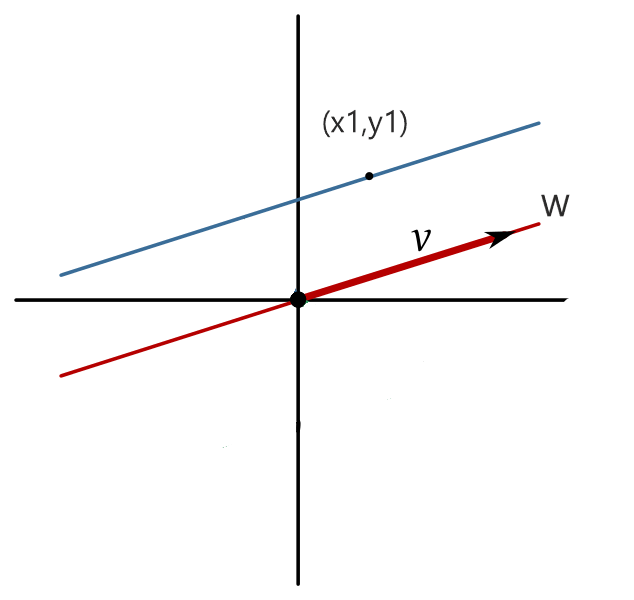
\includegraphics[scale=0.45]{Sistema asociado}
\end{center}

\underline{Demostración}:
\begin{enumerate}
\item Definimos $\phi: K^n\longrightarrow K^m: M_{B_{c_n}, B_{c_m}}(\phi)=A$ donde $B_{c_n}=\{e_1, ..., e_n\}$ y $B_{c_m}=\{e_1', ..., e_m'\}$. De este modo, $v=(x_1, ..., x_n)\in K^n\Rightarrow \phi(v)=(x_1', ..., x_m')\in K^m\Rightarrow \begin{pmatrix}
x_1' \\ \vdots \\ x_m'
\end{pmatrix}=A\cdot \begin{pmatrix}
x_1 \\ \vdots \\ x_n
\end{pmatrix}$.

Ahora vemos que si el sistema es compatible, entonces hay al menos un vector solución cuya imagen\footnote{Porque multiplicar por la matriz $A$ es como aplicar $\phi$} por $\phi$ es $(b_1, ..., b_m)$, por lo que:
$$\Sigma_b(K)\neq \emptyset \Leftrightarrow (b_1, ..., b_m)_{B_{c_m}}\in Im(\phi)\Leftrightarrow b_1e_1'+...+b_me_m'\in Im(\phi)=L\left(\phi(e_1), ..., \phi(e_m)\right)\Leftrightarrow $$
$$\Leftrightarrow L\left(b_1e_1'+...+b_me_m',\phi(e_1), ..., \phi(e_m)\right)=Im(\phi)\Leftrightarrow \dim L=\dim Im(\phi)\Leftrightarrow rg(\phi)=rg(A\mid B)\Leftrightarrow$$
$$\Leftrightarrow rg(A)=rg(A\mid B)$$

\item Sea $(a_1, ..., a_n)\in \Sigma_b(K)$ y $(c_1, ..., c_n)\in \Sigma_0(K)$, entonces vemos que:
$$A\cdot \begin{pmatrix}
a_1 \\ \vdots \\ a_n
\end{pmatrix}=B, A\cdot \begin{pmatrix}
c_1 \\ \vdots \\ c_n
\end{pmatrix}=0 \Rightarrow (a_1+c_1, ..., a_n+c_n)\in \Sigma_b(K)\Rightarrow A\cdot \begin{pmatrix}
a_1+c_1 \\ \vdots \\ a_n+c_n
\end{pmatrix}=\begin{pmatrix}
b_1+0 \\ \vdots \\ b_n+0
\end{pmatrix}=\begin{pmatrix}
b_1 \\ \vdots \\ b_n
\end{pmatrix}$$
\end{enumerate}

\subsection*{\underline{Regla de Cramer}}
Para la resolución de sistemas lineales que sean compatibles determinados, existe un método muy eficiente conocido como la \textit{regla de Cramer}:
$$\Sigma:\begin{cases}a_1x+b_1y+c_1z=d_1 \\ a_2x+b_2y+c_2z=d_2 \\ a_3x+b_3y+c_3z=d_3 \end{cases}\Rightarrow \left( x=\frac{\begin{vmatrix} d_1 & b_1 & c_1 \\ d_2 & b_2 & c_2 \\ d_3 & b_3 & c_3 \end{vmatrix}}{|A|}, y=\frac{\begin{vmatrix} a_1 & d_1 & c_1 \\ a_2 & d_2 & c_2 \\ a_3 & d_3 & c_3 \end{vmatrix}}{|A|}, z=\frac{\begin{vmatrix} a_1 & b_1 & d_1 \\ a_2 & b_2 & d_2 \\ a_3 & b_3 & d_3 \end{vmatrix}}{|A|} \right)$$

\underline{Demostración}:

\chapter*{ESTRUCTURA DE \\ ENDOMORFISMOS}
Vamos a estudiar en este tema la estructura de unas aplicaciones lineales muy concretas, las que van de un cuerpo en sí mismo.

\subsection*{\underline{Matrices semejantes}}
Supongamos que $\dim V = n$, $B=\{v_1, ..., v_n\}$ base de $V$ y que $\phi: V\rightarrow V$.

Dada la aplicación lineal, esta queda definida por su matriz: $A=M_B(\phi)$ y tenemos que la matriz respecto de otra base queda relacionada con la anterior por la siguiente fórmula:
$$A'=M_B'(\phi): A'= P^{-1}AP: P=M(B',B)\in Gl_n(K)$$

Estas dos matrices $A$ y $A'$ son \textbf{semejantes} cuando se relacionan de este modo y de nuevo definen una relación de equivalencia entre matrices.\footnote{Muy semejante a la relación de equivalencia que vimos en el tema anterior}. La intención de este capítulo es clasificar los endomorfismos según su clase de equivalencia de la forma definida previamente.

\section*{POLINOMIO MÍNIMO Y CARACTERÍSTICO DE \\UN ENDOFMORFISMO}
\subsection*{\underline{Polinomio mínimo de una matriz}}
Consideramos $A\in Mat_n(K)$ y el conjunto de vectores $\{I_n, A, A^2, ..., A^{n^2}\}\subset Mat_n(K)$.

Como $\dim Mat_n(K)= n^2$ y tenemos en ese conjunto $n^2+1$ vectores, necesariamente ese conjunto es linealmente dependiente. Con lo cual, $\exists a_0, ..., a_{n^2}\in K: a_0I+...+a_{n^2}A^{n^2}=0$ donde $\exists a_i \neq 0$.

Esto se puede interpretar como que $A$ es la raíz de un polinomio luego:
$$(a_0+a_1x+...+a_{n^2}x^{n^2})(A)=f(A): f\neq 0$$

Luego tal y como vimos en el tema de polinomios, podemos considerar que $A$ es la matriz compañera del polinomio definido por la dependencia lineal de dicho conjunto de vectores.

\subsubsection*{Proposición}
Dada una matriz cuadrada siempre existe un polinomio no nulo y de grado al menos 1 del que es raíz.
$$A\in Mat_n(K)\Rightarrow \exists f\in K[x]: f(A)=0$$

\subsubsection*{Proposición}
Dada una matriz en las condiciones anteriores, existe un único polinomio de manera que ese es mínimo:
$$\exists! q_A\in K[x]:$$
\begin{itemize}
\item $q_A\neq 0$
\item $q_A \mbox{ mónico }$
\item $q_A(A)=0$
\item $f(A)=0\Rightarrow q_A\mid f$
\end{itemize}

\underline{Demostración}:\par
Las tres primeras condiciones ya se han visto donde se explica la parte de como descubrir dicho polinomio, por lo que vamos a demostrar la 3ª:
$$f(A) = 0 \Rightarrow f(A)=0= g(A)q_A(A)+r(A)\Rightarrow r(A)=0\Rightarrow r=0\Rightarrow q_A\mid f$$
Vemos que $r(A)=0\Rightarrow r=0$ porque $q_A$ es mínimo, entonces $r(A)$ que es de grado más pequeño no puede anularse a menos que sea el polinomio nulo.

Veamos que es único:
$$q_A, q_A'\Rightarrow q_A\mid q_A' \mbox{ pero también }q_A'\mid q_A \Rightarrow q_A = q_A'$$

\subsubsection*{Proposición: polinomio mínimo de matrices semejantes}
Supongamos que tenemos $A\sim A'$, veamos que ocurre con $q_A(A')$, vemos que:
$$q_A(A')=q_A(P^{-1}AP)= (a_0+a_1x+...+x^m)(P^{-1}AP)= a_0I+a_1P^{-1}AP+...+(P^{-1}AP)^m= $$
$$= a_0I+P^{-1}a_1AP+...+ P^{-1}A^mP= P^{-1}(a_0I+a_1A+...+A^m)P = P^{-1}\underbrace{q_A(A)}_{=0}P = 0$$

Luego tenemos que matrices semejantes tienen el mismo polinomio mínimo.

\subsection*{\underline{Polinomio mínimo de un endomorfismo}}
Con los resultados anteriores, podemos definir el polinomio mínimo como el polinomio que define al endomorfismo, \textbf{sea cual sea la matriz que lo representa}.

Ej.:
Sea $f\in K[x]$ mónico, donde f es no constante$\Rightarrow C_f\Rightarrow q_{C_f}=f$ donde $C_f$ es la matriz compañera del polinomio $f$.

Si $\phi$ es proyección entonces $\phi^2= \phi\Leftrightarrow (x^2-x)(\phi)= 0\Leftrightarrow q_\phi = \begin{cases} x(\phi) = 0 & \Rightarrow \phi = 0 \\ (x-1)(\phi) = 0 & \Rightarrow\phi = id \\ (x^2-x)(\phi) = 0 & \Rightarrow\phi \neq 0,id\end{cases}$.

Si $\phi$ es simetría, entonces tenemos que: $\phi^2=id\Leftrightarrow (x^2-1)(\phi)=0\Leftrightarrow \begin{cases} (x-1)(\phi) = 0 & \Rightarrow \phi = id \\ (x+1)(\phi) = 0 & \Rightarrow \phi = -id \\ (x^2-x)(\phi) = 0 & \Rightarrow\phi \neq 0,-id\end{cases}$.

Supongamos que $q_\phi = (x-1)(x-r): r\neq 0, 1, -1$ donde decimos que este endomorfismo es una homología general de razón $r$.

\subsection*{\underline{Polinomio mínimo de un endomorfismo y un vector}}
Vemos que el polinomio mínimo de un endomorfismo se anula en ese endomorfismo: $q_\phi(\phi)=0$. Del mismo modo, si sustituimos un endormorfismo en un polinomio y vemos la matriz de esa evaluación vemos que:
$$M_B(f(\phi)): f= a_0+...+a_mx^m \Rightarrow f(\phi)= a_0 id_v+...+a_m\phi^m\Rightarrow$$
$$\Rightarrow M_B(f(\phi))=a_0I+a_1A+...+a_mA^m= f(A):A=M_B(\phi)$$
Con lo cual vemos que la matriz en base $B$ de $f(\phi)$ es justamente evaluar $A$ en $f$, es decir, $f(A)$.

Entonces vemos que para que el endomorfismo $q_\phi(\phi) = 0$ sea el endomorfismo nulo, su matriz en cualquier base ha de ser la matriz nula, es decir:
$$q_\phi (\phi)=0\Leftrightarrow M_B(q_\phi(\phi))= 0\Leftrightarrow M_B(q_A(\phi))=0 \Leftrightarrow q_A(A)=0$$


Esto nos permite ver $q_\phi(\phi)$ como el endomorfismo nulo o como la matriz nula de la forma que mejor nos convenga. Lo que implica que si es el endomorfismo nulo, el polinomio mínimo de $\phi$ se anula en cualquier $\phi(v)$, luego: $[q_\phi(\phi)](v)=0$

Es decir, ahora podemos redefinir el polinomio mínimo, pero ahora respecto de dos objetos $q_{\phi, v}$ siendo $v\in V: v\neq 0$.

Este polinomio es el único polinomio mónico no nulo en $K[x]$ tal que $[q_{\phi,v}(\phi)](v)=0$, por lo tanto $q_\phi,v\mid q_\phi$.

Ej.:

Imaginemos que tenemos una proyección cuya matriz respecto de la base canónica es $M_{B_c}(\phi)=\begin{pmatrix} 1 & 0 \\ 0 & 0\end{pmatrix}$, ¿cuál es el polinomio mínimo de esta proyección? Por todo lo desarrollado antes es fácil ver que $q_\phi(\phi)= x^2-x$, pero ¿quién es $q_{\phi,e_1}(\phi)$ y $q_{\phi, e_2}$?.

Aplicamos la proyección al primer vector y segundo vector: $\phi(e_1)=e_1$ y $\phi(e_2)=0$. Entonces $q_{\phi,e_1}=x-1(\phi)$ y $q_{\phi, e_2}=x$ porque $(x-1)(\phi)=\phi-id$ y ahora $\phi(e_1)-id(e_1)=e_1-e_1=0$, es decir, al evaluar $e_1$ en $q_{\phi,e_1}$ obtenemos que el resultado es 0. Del mismo modo que con $(x)(\phi)=\phi$ y ahora $\phi(e_2)=0$.

\subsubsection*{Proposición}
Del hecho anterior, se desprende una consecuencia inmediata: el mcm de los $q_{\phi,v_i}$ tales que estos $v_i$ son la base del espacio vectorial, es precisamente $q_\phi$:
$$q_\phi = mcm\{q_{\phi, v_1}, ..., q_{\phi, v_n}\}: B=\{v_1, ..., v_n\} \mbox{ es base}$$

\underline{Demostración:}
Vamos a ver que $q_\phi = \bar{q}$ y para ello basta con ver que se dividen mutuamente, es decir, que $q_\phi \mid \bar{q}$ y $\bar{q}\mid q_\phi$: 

$$q_i\mid q_\phi\Rightarrow \bar{q}\mid q_\phi$$
Por otro lado:
$$\bar{q}= q_i\cdot g_i: i=1,2,...,n$$

Con lo cual, vemos que le pasa a $\bar{q}(\phi)$ cuando se le aplica a $v_i$:
$$\left[\bar{q}(\phi)\right](v_i)=\left[(g_iq_i)(\phi)\right](v_i)= [g_i(\phi)\circ q_i(\phi)](v_i)=g_i(\phi)\left(\underbrace{q_i(\phi)(v_i}_{=0})\right) = g_i(\phi)(0)=0\Rightarrow \left[\bar{q}(\phi)\right](v_i)==0$$

Por tanto, $\bar{q}(\phi)$ es la aplicación nula porque se anula sobre cada uno de los vectores de la base, luego $q_\phi \mid \bar{q}$.

\subsubsection*{Cálculo del polinomio mínimo}
Con lo cual, en la práctica, basta con calcular el polinomio mínimo de cada uno de los vectores de la base del espacio vectorial; puesto que el buscado es el m.c.m. de ellos. Además, la búsqueda del polinomio mínimo de cada vector se puede plantear de la siguiente forma: como lo que se busca es una expresión $a_0v+a_1\phi(v)+...+a_n\phi^n(v_n)$ de tamaño mínimo y con algún $a_i\neq 0$, entonces si hallamos $v,\phi(v), \phi^2(v),... \in V$ en algún momento el número de vectores será mayor que la dimensión de la base (o incluso antes lo veremos) y entonces serán linealmente dependientes, luego tendremos cada $a_i$.

Ej.:

Sea $M_B(\phi)=\begin{pmatrix} 0&1&1\\1&0&1\\1&1&0\end{pmatrix}$, vemos que $\phi(e_1) = e_2+e_3$ y $\phi^2(e_1)=2e_1+e_2+e_3$. Vemos incluso que antes de que el número de vectores sea mayor que la dimensión de $R^3$ ya tenemos una colección de vectores que guardan dependencia lineal de la siguiente forma: $\phi^2(v)-2e_1-2\phi(e_1)=0$, luego tenemos que $[(x^2-x-2)(\phi)](e_1)=0$ luego $q_{\phi,e_1}=x^2-x-2$.
Realizando este procedimiento con el resto de vectores y hallando el m.c.m. tenemos el $q_\phi$.

\subsection*{\underline{Polinomio característico}}
\subsubsection*{Autovalores y autovectores}
Sea $\lambda\in K$ y $v\neq 0$, se tiene que:
$$q_\phi(\lambda)=0\Leftrightarrow \exists v\neq 0: \phi(v)=\lambda\cdot v \Leftrightarrow |A-\lambda\cdot I_n|=0$$
Siendo $A$ la matriz del endomorfismo en \textbf{cualquier base}.

Es decir, las \textbf{raíces del polinomio mínimo} son los autovalores del endomorfismo y los vectores que verifican $\phi(v)=\lambda \cdot v$ son los \textbf{autovectores} del endomorfismo.

\underline{Demostración}:

2 implica 1:
$$\phi(v)-\lambda v =0 \Rightarrow q_{\phi,v}=x-\lambda \Rightarrow x-\lambda\mid q_\phi\Rightarrow q_\phi(\lambda)=0$$

1 implica 2:
$$q_\phi(\lambda)=0\Rightarrow x-\lambda\mid q_\phi\Rightarrow q_\phi = (x-\lambda)g(x)$$
Sea $B=\{v_1, ..., v_n\}$ una base consideremos $q_i=q_{\phi,v_i}$, entonces si $x-\lambda \nmid q_1, ..., q_n \Rightarrow x-\lambda\nmid mcm\{q_1, ..., q_n\}$ pero ocurre que $q_\phi = mcm \{...\}$ luego necesariamente $x-\lambda \mid q_i$ para algún $i \in \mathbb N$. Por tanto, se tiene (podemos escoger que es $q_1$ porque el orden no importa) que $q_1=q_{\phi,v_i} = (x-\lambda)h(x)$. Esto necesariamente conlleva a que $(\phi-\lambda\cdot id)(h(\phi)(v_1))=0$, $h(\phi)(v_1)$ no puede ser 0 porque sería el polinomio mínimo de $v_1$ y no lo es luego precisamente $h(\phi)(v_1)=v$, es decir, es el vector donde se cumple la desigualdad.   

2 implica 3

Si expresamos en términos de una base $B=\{v_1,..., v_n\}$ de forma que queda $v=a_1v_1+...+a_nv_n$ vemos que como $\phi(v)=\lambda\cdot v$ se ve fácilmente que $(A-\lambda\cdot I_n)(v)=0$, luego como ese sistema tiene solución no nula el determinante de la matriz del sistema es 0, por lo tanto tenemos que $|A-\lambda \cdot I_n|=0$

\subsubsection*{\underline{Polinomio característico}}
Llamamos polinomio característico de $A$ o $p_A$ a:
$$|A-\lambda I_n|=|A-x\cdot I_n|(\lambda)=p_A(\lambda)=0$$
De hecho, este polinomio representa al endomorfismo sea cual sea la base en la que esté expresado, es decir, no depende de la matriz $A$, por lo que tiene sentido llamarlo $p_\phi$.

El grado del polinomio característico es $gr(p_\phi)=n: \dim V=n$ y además es de la forma: $p_\phi= (-1)^nx^n+(-1)^{n-1}tr(A)+(-1)sx+...+|A|$, donde $s$ son los determinantes de orden dos en los que aparece un término de la diagonal\footnote{Los demás términos intermedios del polinomio se obvian, pero existen fórmulas para interpretar los coeficientes en cada grado.}.

\underline{Demostración}:

Sean $A=M_B(\phi)$ y $A'=M_B'(\phi)$, ambas matrices por ser semejantes cumplen que $A'=P^{-1}AP$. Veamos que:
$$p_{A'}=|A'-xI_n|=|P^{-1}AP-P^{-1}xP|=|P^{-1}(A-xI_n)P|=|P^{-1}|(A-xI_n)|P|=|(A-xI_n|=p_A$$

Luego si $q_\phi(\lambda)=0\Leftrightarrow|A-\lambda I_n|=0\Leftrightarrow p_\phi(\lambda)=0$, entonces las raíces de $q_\phi$ son raíces de $p_\phi$ y viceversa, luego son el mismo polinomio salvo multiplicidad de raíces.


\subsubsection*{Subespacios propios}
Si definimos por $V_{\phi, \lambda}$ como el subespacio de $V$ en el que todos los vectores cumplen $\phi(v)=\lambda v$, vemos que realmente estamos diciendo que $Ker(\phi-\lambda id)=V_{\phi,\lambda}$. Esto es lo que definimos como \textbf{subespacio propio}:
$$V_{\phi,\lambda}=Ker(\phi-\lambda\cdot id_V)=\{v\in V: \phi(v)=\lambda \cdot v\}<V$$
Es trivial ver que es un subespacio puesto que como se trata del $Ker$ de una aplicación lineal, este siempre es un subespacio vectorial del espacio en el que esta definido el endomorfismo.

Si $V_{\phi,\lambda}\neq 0\Rightarrow \lambda\mbox{ es autovalor y }v\in V_{\phi,\lambda}\mbox{ es un vector propio}$.

Vamos a llamar al conjunto de los autovalores a $\sigma(\phi)=\{\lambda_1, ..., \lambda_t\}: q_\phi(\lambda_i) = 0$ y se denota por el \textbf{espectro}.

\subsection*{\underline{Teorema de Caley - Hamilton}}
Todo endomorfismo es raíz de su polinomio característico, es decir,
$$p_\phi (\phi) = 0$$

\underline{Demostración}

La demostración de este teorema consiste en probar que el polinomio mínimo siempre divide al polinomio característico:
$$q_\phi | p_\phi$$
Porque implica directamente que $p_\phi (\phi) = 0$

\subsubsection*{Lema}
Si $f \in K[x]$ es un polinomio irreducible, y $f^a$ es la potencia exacta que divide a $q_\phi$, entonces
$$f^a || q_\phi, \ f^a | q_\phi, \ f^{a+1} \nmid \mid q_\phi \Rightarrow f^a | p_\phi$$

\underline{Demostración}

Sea $B = \{v_1, \ldots, v_n \}$ base de $V$. Llamamos $q_i = q_{\phi, v_i}$

Sabemos que $q_\phi = mcm \{q_1, \ldots, q_n\}$. Queremos ver que hay vectores en $V$ cuyo polinomio mínimo es exactamente $f^a$. Razonamos por reducción al absurdo.

Supongamos $q_i = f^{a_i} g_i \mbox{ tal que }$
$$f^{a_i} || q_i : a_1 \leq a_2 \leq \ldots \leq a_n \leq a$$

Supongamos que $a_n < a$. Entonces $ mcm \{q_1, \ldots, q_n\} = f^{a_n}  \cdot mcm \{g_1, \ldots, g_n\}$. Sin embargo, esto es una contradicción ya que $mcm \{q_1, \ldots, q_n\} = q_\phi$, y por hipótesis $f^a | q_\phi$, pero $a_n < a $.

Por tanto, $a_n = a$
$$\Rightarrow q_{\phi, v_n} = f^a \cdot g_n \Rightarrow 0 = f^a(\phi)(\underbrace{g_n(\phi)(v_n)}_{v \neq 0}) \Rightarrow q_{\phi, v} = f^a $$
Ya que si $v = 0, q_{\phi, v_n}$ sería como mucho $g_n$, pero $g_n$ es menor que el mínimo.

Por tanto, $\exists v \in V, v \neq 0 : q_{\phi, v} = f^a$

Llamamos $m = gr(f^a)$. Por las propiedades del polinomio mínimo, sabemos que $\nexists f \in K[x] , gr(f) < m : f_{\phi, v} = 0$.

Veamos que los vectores $\{v, \phi(v), \ldots, \phi^{m-1}(v)\}$ son linealmente independientes. Supongamos
$$ 0 = a_0 v + a_1 \phi(v) + \ldots + a_{m-1}\phi^{m-1}(v) $$
$$0 = \left[(a_0  + a_1 x + \ldots + a_{m-1}x^{m-1})(\phi)\right](v)$$
Sin embargo, estamos diciendo que el polinomio $a_0  + a_1 x + \ldots + a_{m-1}x^{m-1}$ que sobre $\phi(v)$ vale 0, pero su grado es menor que m, que es el grado del mínimo, lo cual es imposible salvo que el polinomio sea nulo.
$$a_1 = \ldots = a_{m-1} = 0$$
Extendemos ahora estos $m$ vectores independientes a una base de todo el espacio.
$$B = \{ v, \phi(v), \ldots, \phi^{m-1}(v), v_{m+1}, \ldots, v_n \} \mbox{ base de $V$}$$
Veamos que $f^a | p_\phi$.

$$v \mapsto \phi(v) , \phi(v) \mapsto \phi^2(v), \ldots, \phi^{m-1}(v) \mapsto \phi^m(v) $$
Los primeros vectores de la base van al siguiente de la base, excepto el $\phi^{m-1}(v)$, que va a $\phi^m(v)$. Estudiamos dicha imagen.

$$m= gr(f^a) \Rightarrow f^a = x^m + b_{m-1}x^{m-1} + \ldots + b_0  \Rightarrow \phi^m(v) + b_{m-1} \phi^{m-1} (v) + b_1 \phi(v) + b_0 v = 0$$
$$\phi(\underbrace{\phi^{m-1}(v)}_{v_m}) = \phi^m (v) = -b_0 v - b_1 \phi(v) - \ldots - b_{m-1} \phi^{m-1} (v) $$

$$A = M_B (\phi) = \left(\begin{array}{c|c}
C_{f^a} & M \\
\hline
0 & N   \\
\end{array}
\right)$$

$p_\phi = |A - xI_n| = \left|\begin{array}{c|c}
C_{f^a} - xI_m & M \\
\hline
0 & N - xI_{n-m}  \\
\end{array}
\right| \overset{\mbox{Triangular inferior}}{=} |C_{f^a} - xI_m| \cdot |N - xI_{n-m}| = p_{C_{f^a}} \cdot p_N = \pm f^a \cdot p_N$

Por tanto, $f^a | p_\phi$
$\hfill\square$

A partir de aquí, tenemos
$\begin{cases} q_\phi = f^{a_1}_1 \cdot \ldots \cdot f^{a_t}_t \\
\pm p_\phi =  f^{e_1}_1 \cdot \ldots \cdot f^{e_t}_t \cdot f^{e_{t+1}}_{t+1} \cdot \ldots \cdot f^{e_s}_s  \end{cases} 1  \leq a_i \leq e_i$

Veamos que los factores $f^{e_{t+1}}_{t+1} \cdot \ldots \cdot f^{e_s}_s $ no pueden existir, es decir, que si $f \in K[x]$ irreducible y $f | p_\phi \Rightarrow f | q_\phi$. La idea de la demostración se basa en la reducción al caso de que $f$ fuera de grado 1, utilizando la técnica de extensión del cuerpo a un cuerpo mayor donde sabemos que $f$ descompone completamente.

Sea $K \subset \tilde{K} : p_\phi $ descompone completamente en $\tilde{K}[x]$. Sea $A = M_B (\phi) \in Mat_n(K) \subseteq Mat_n(\tilde{K})$

Sea $\tilde{V} = \tilde{K}^n$ un $\tilde{K}$- espacio vectorial. En este espacio $\tilde{K}^n$ fijamos la base $\tilde{B_c}$.

Definimos $\tilde{\phi} \in End(\tilde{K}^n)$ tal que $M_{\tilde{B_c}}(\tilde{\phi}) = A$. Se cumple que:
\begin{itemize}
\item $p_{\tilde{\phi}} = |A - xI_n| = p_\phi$

\item $\tilde{K}[x] \ni q_{\tilde{\phi}} | q_\phi \in K[x]$
\end{itemize}

Razonamos por reducción al absurdo. Supongamos que $f \centernot \mid q_\phi \overset{f \mbox{ irreducible}}{\Rightarrow} 1 = mcd(f, q_\phi)$. Por Bézout:
$$1 = a\cdot f + b \cdot q_\phi$$
Por otra parte, ya hemos probado que $p_\phi = p_{\tilde{\phi}} \mbox{ y } q_{\tilde{\phi}}$ tienen las mismas raíces. Sea $$\tilde{\lambda} \in \tilde{K} : \underset{ p_{\tilde{\phi}} (\tilde{\lambda}) = 0}{f(\tilde{\lambda})} = 0 \Rightarrow x - \tilde{\lambda} | f$$
Sea $\tilde{v} \neq 0 : \tilde{\phi} (\tilde{v}) = \tilde{\lambda} \cdot \tilde{v}$, es decir, que $\tilde{v}$ es vector propio del autovalor $\tilde{\lambda}$. Descomponiendo $f = g(x)(x-\tilde{\lambda})$ tenemos que:
$$1 = a(x)g(x)(x-\tilde{\lambda}) + b(x)q_\phi (x) $$
Usando el endomorfismo $\tilde{\phi}$:
$$id_{\tilde{V}} = a(\tilde{\phi})\circ g(\tilde{\phi}) \circ(\tilde{\phi} - \tilde{\lambda} \cdot id_{\tilde{V}}) + b(\tilde{\phi}) \circ q_\phi (\tilde{\phi})$$
OBS: $q_\phi (\tilde{\phi}) = 0$
$$id_{\tilde{V}} = a(\tilde{\phi})\circ g(\tilde{\phi}) \circ(\tilde{\phi} - \tilde{\lambda} \cdot id_{\tilde{V}})$$

Aplicamos esta identidad entre aplicaciones lineales al vector $\tilde{v}$ elegido previamente:
$$\tilde{v} = id_{\tilde{V}} (\tilde{v})= a(\tilde{\phi})\left( g(\tilde{\phi})( \tilde{\phi}(\tilde{v}) - \tilde{\lambda}\tilde{v})\right)$$
Por construcción de $\tilde{v} : \tilde{\phi}(\tilde{v}) - \tilde{\lambda}\tilde{v} = 0$
$$\tilde{v} = a(\tilde{\phi})\left( g(\tilde{\phi})( \tilde{\phi}(0)\right) = 0 (!)$$

Por tanto, todos los irreducibles de $q_\phi$ y de $p_\phi$ son los mismos, cambiando únicamente los exponentes. Así, $$q_\phi | p_\phi$$
$\hfill\square$

\subsubsection*{Proposición}
Sea $q_\phi$ el polinomio mínimo y $p_\phi$ el polinomio característico, entonces poseen los mismos irreducibles en su descomposición salvo la multiplicidad de estos, que es mayor en la del característico.
$$1\leq a_i\leq e_1: q_\phi = f_1^{a_1} \cdot ... \cdot f_t^{a_t} \wedge \pm p_\phi=f_1^{e_1} \cdot ... \cdot f_t^{e_t}\cdot f_{t+1}^{e_{t+1}} \cdot ... \cdot f_{s}^{e_s}$$

\underline{Demostración}:

Sea $q_\phi = f_1^{a_1} \cdot ... \cdot f_t^{a_t}$ y $\pm p_\phi=f_1^{e_1} \cdot ... \cdot f_t^{e_t}\cdot f_{t+1}^{e_{t+1}} \cdot ... \cdot f_{s}^{e_s}$. Vamos a ver que estos factores adicionales no pueden existir, y en consecuencia solo cambian los exponentes de cada factor irreducible, pero no los factores irreducibles. Para ello basta con demostrar que $f\mid p_\phi\Rightarrow f\mid q_\phi$

Sea $f\in K[x]: f$ es irreducible y $f\mid p_\phi \Rightarrow f\mid q_\phi$. Vamos a extender el cuerpo $K$ a un cuerpo $\tilde{K}$ de manera que $K\subset \tilde{K}$ y $p_\phi$ descompone en $\tilde{K}[x]$. Entonces tenemos que la matriz de A también tiene sentido en $\tilde{K}$: $A=M_B(\phi)\in Mat_n(K)\subset Mat_n(\tilde{K})$. Si fijamos una base en un espacio del nuevo cuerpo, entonces ahora $A$ puede representar la matriz de otro endomorfismo dentro de ese cuerpo, por lo que ahora si llamamos $\tilde{V}=\tilde{K}^n$ donde es $\tilde{K}-$espacio vectorial y definimos $\tilde{B}_c$ podemos considerar $\tilde{\phi}\in End(\tilde{K}^n): M_{\tilde{B}_c}(\tilde{\phi})=A$.

Ahora tenemos que $p_{\tilde{\phi}}= |A-x\cdot I_n|$, pero este mismo polinomio es el de $\phi$, luego $p_{\tilde{\phi}}= |A-x\cdot I_n|=p_\phi$. Del mismo modo, tenemos que $q_{\tilde{\phi}}\in \tilde{K}[x]$ y $q_\phi\in K[x]$, pero por el cuerpo al que pertenece cada uno se tiene que $q_{\tilde{\phi}}\in \tilde{K}[x]\mid q_\phi\in K[x]$

Por reducción a lo absurdo, supongamos que $f\nmid q_\phi$, este caso como $f$ es irreducible, entonces $1=mcd(f,q_\phi)$ y por el Teorema De Bezout se tiene que $1=a\cdot f + b \cdot q_\phi$.

Por otro lado, sabemos que $p_{\tilde{\phi}}$ y $q_{\tilde{\phi}}$ tienen las mismas raíces, por lo que sea $\tilde{\lambda}\in \tilde{K}: f(\tilde{\lambda})=0$. Como $p_{\tilde{\phi}}=p_\phi$ entonces $f\mid p_{\tilde{\phi}}$ y como $gr(f)\geq 1$ entonces para alguno de estos landa $f(\tilde{\lambda})=0$, lo que implica que $x-\tilde{\lambda}\mid f$ y por tanto $p_{\tilde{\phi}}(\tilde{\lambda})=0$, es decir, $\tilde{lambda}$ es un autovalor. Con lo cual tenemos vectores propios, así que sea $\tilde{v} = 0: \tilde{\phi}(\tilde{v})=\tilde{\lambda}\cdot \tilde{v}$, tenemos recuperando la identidad de Bezout anterior que:
$$1=a(x)g(x)(x-\tilde{\lambda})+ b(x)q_{\phi}(x)\Rightarrow id_{\tilde{v}}=a(\tilde{\phi})\circ g(\tilde{\phi})\circ (\tilde{\phi}-\tilde{\lambda}id_{\tilde{v}})+ b(\tilde{\phi})\circ \underbrace{q_{\phi}(\tilde{\phi})}_{=0}=a(\tilde{\phi})\circ g(\tilde{\phi})\circ (\tilde{\phi}-\tilde{\lambda}id_{\tilde{v}})$$

Si ahora lo aplicamos al $\tilde{v}\neq 0$ elegido previamente tenemos que:
$$\tilde{v}=a(\tilde{\phi})\left(g(\tilde{\phi})\left(\underbrace{\tilde{\phi}-\tilde{\lambda}\tilde{v}}_{=0}\right)\right)\Rightarrow \tilde{v}=0\Rightarrow\#$$


\section*{CLASES NOTABLES DE ENDOMORFISMOS}
\subsection*{\underline{Diagonalizabilidad}}
Decimos que $\phi$ es diagonalizable si existe alguna base de manera que la matriz de $\phi$ en esa base es diagonal.
$$\phi \mbox{ es diagonalizable}\Leftrightarrow \exists B=\{v_1, ..., v_n\}: M_{B}(\phi)\mbox{ sea diagonal}$$

Ej.:

Supongamos que $\phi: V\rightarrow V$ simetría, entonces $V=W\oplus U$ definimos $\dim V=n$, $\dim W=m$ y $\dim U = m-n$. Escogemos una base de $V$, $B=\{\underbrace{v_1, ..., v_m,}_{B_W} \underbrace{v_{m+1}, ..., v_n}_{B_U}\}$ vemos que como un endomorfismo queda determinado por la imagen de los vectores de la base:
$$M_B(\phi)=\begin{pmatrix}
I_n & | & 0 \\ - & + & - \\ 0 & | & -I_{n-m}
\end{pmatrix}$$
Lo que ocurre realmente es que si $A=M_{B'}(\phi)$ y $A=M_B(\phi)$, entonces $\exists P=M(B',B): A'=P^{-1}AP$. Es decir, transformo mediante una matriz de paso, una matriz que no es diagonal en una \textbf{semejante} que sí lo es.

\subsubsection*{Proposición}
Una $\phi$ es diagonalizable si y sólo si $V$ posee alguna base formada por vectores propios.

Luego esto nos da un muy buen criterio para saber si un endomorfismo es diagonalizable puesto que sabemos hallar autovectores y bases.

\underline{Demostración}:
\begin{itemize}
\item $\Rightarrow$

$$\exists B=\{v_1, ..., v_n\} : M_B(\phi)=D=\begin{pmatrix}
\lambda_1 & \cdots & 0 \\
\vdots & \ddots & \vdots \\
0 & \cdots & \lambda_n
\end{pmatrix}\Rightarrow \phi(v_i)=\lambda_i \cdot v_i\Rightarrow v_i \mbox{ autovector}$$

\item $\Leftarrow$
$$B\mbox{ base}: \phi(v_i)=\lambda_iv_i: i=1,..., n\Rightarrow M_B(\phi)=\begin{pmatrix}
\lambda_1 & \cdots & 0 \\
\vdots & \ddots & \vdots \\
0 & \cdots & \lambda_n
\end{pmatrix}$$
\end{itemize} 

Ej.:

Supongamos que $M_{B_c}(\phi)=\begin{pmatrix}
0&1&1\\1&0&1\\1&1&0
\end{pmatrix}$ luego tenemos $p_\phi= (x+1)^2(x-2)$ y $q_\phi=(x+1)(x-2)$, por lo que tenemos que $\lambda_1 = -1$ y $\lambda_2 = 2$ y tenemos que $V_{\phi, \lambda_1}= Ker(\phi+id): (A+I_3)$ cuyo resultado del sistema es $V_{\phi, \lambda_1}:x+y+z=0$. Es decir, como es un plano puedo encontrar en él dos vectores linealmente independientes.

Vamos a por el segundo $V_{\phi,\lambda_2}=Ker(\phi-2id)$ y al final tenemos que $V_{\phi,\lambda_2}:\begin{cases}x-2y+z=0 \\ x+y-2z=0\end{cases}$, que por ser una recta posee un vector linealmente independiente.

Así que uniendo los 3 vectores comentados se tiene que $B'=\{(e_1-e_2), (e_1-e_3), (e_1+e_2+e_3)\}$ es base de $V$. Expresando $\phi$ en la base construida se tiene que $A'=M_{B'}(\phi)=\begin{pmatrix}-1&0&0\\0&-1&0\\0&0&2\end{pmatrix}$.

\subsubsection*{Propiedad}
Vectores propios no nulos respecto de autovalores distintos forman conjuntos linealmente independientes.
$$v_1\in V_{\phi, \lambda_1}, v_2\in V_{\phi,\lambda_2}: \lambda_1 \neq \lambda_2\Rightarrow \{v_1,v_2\}\mbox{ linealmente independientes}$$

\underline{Demostración}:

$$a_1v_1+a_2v_2=0\Rightarrow \phi(a_1v_1+a_2v_2)=\phi(0)=0\Rightarrow a_1\lambda_1v_1+a_2\lambda_2v_2=0$$
Por otro lado tenemos que:
$$a_1v_1+a_2v_2=0\Rightarrow a_1\lambda_1v_1+a_2\lambda_1v_2=0$$
Restando ambas:
$$a_2(\lambda_2-\lambda_1)v_2=0\Rightarrow a_2=0$$
Y tenemos que $a_1v_1=0\Rightarrow a_1=0$

\subsubsection*{Proposición}
Supongamos que $\phi$ es diagonalizable, entonces su matriz es diagonal, es decir, $A=\begin{pmatrix}\lambda_1 &\cdots &0\\ \vdots &\ddots & \vdots\\ 0 &\cdots &\lambda_n\end{pmatrix}$ por lo que vemos que su polinomio característico es $p_\phi = |A-x\cdot I_n|=(\lambda_1-x)\cdots (\lambda_n-x)=(-1)^n\cdot (x-\lambda_1)\cdots (x-\lambda_n)$.

En primer lugar, \textbf{el polinomio característico de un endomorfismo diagonalizable descompone completamente en $K[x]$}.
$$p_\phi=(-1)^{n}(x-\lambda_1)\cdot ... \cdots (x-\lambda_n)$$

En segundo lugar, \textbf{la diagonal de un endoformismo diagonalizado es precisamente el espectro del mismo}.

Por último, Si un endomorfismo es diagonalizable, su polinomio mínimo no posee raíces múltiples y descompone completamente.

\underline{Demostración}:

Si tenemos que $(-1)^n\cdot (x-\lambda_1)\cdots (x-\lambda_n)$, la hipótesis es que el mínimo posee los mismos factores pero sin repetir, es decir, $q_\phi= (x-\lambda_1)\cdot ... (x-\lambda_t)$ donde $t$ es el número de raíces distintas. Vamos a ver que realmente $q_\phi(\phi)=0$.

Tenemos que por los teoremas anteriores, hay una base formada por autovectores de forma que $B=\{\underbrace{v_{11}, ..., v_{m1}}_{\in V_{\phi, \lambda_1}}, ...\}$, ahora nos preguntamos:
$$[(x-\lambda_1)\cdot ... \cdot (x-\lambda_t)](\phi)(v_{1j})=[(x-\lambda_2)\cdot ... \cdot (x-\lambda_t)(x-\lambda_1)](\phi)(v_{1j})=[(\phi-\lambda_2 id)\cdot ... \cdot (\phi-\lambda_t id )](\underbrace{\phi-\lambda_1 id)(v_ij}_{\lambda_1 v_{ij}-\lambda_1v_{1j}=0})=0$$
Si hacemos lo mismo con el resto de autovalores se tiene que el polinomio que hemos definido se anula completamente sobre los vectores de una base, es decir, que $q_\phi(\phi)=0$.

\subsubsection*{Proposición}
$\phi$ es diagonalizable si y solo si $p_\phi$ descompone en $K[x]$ de forma que $d_i = e_i$.

\subsubsection*{Potencia enésima de matrices}
Una aplicación bastante buena de esta parte de teoría es hallar la fórmula general de la sucesión geométrica cuyo término base es la matriz A. Para ello hay que distinguir dos casos:
\begin{itemize}
\item \underline{\textbf{Diagonalizable}}

Este caso es el más sencillo puesto que sabemos que si una matriz es diagonalizable, es posible convertirla en su matriz diagonal asociada a través de una matriz de cambio de base.

Da la casualidad de que la potencia enésima de una matriz diagonal es muy fácil de calcular por lo que es relativamente sencillo calcular el término general de la matriz diagonal y después transformar a la matriz original a través de esa matriz de paso.

Ej.:

Sea $A=\begin{pmatrix}-7&-6\\12&10\end{pmatrix}$ su polinomio característico es $p_\phi=(x-2)(x-1)$, luego su matriz diagonal es:
$D=\begin{pmatrix}2&0\\0&1\end{pmatrix}$. El término general para la matriz diagonal es $D^n=\begin{pmatrix}2^n&0\\0&1^n\end{pmatrix}$ luego a través de la matriz de cambio de base $P=M(B,B')=\begin{pmatrix}
-4&-3\\3&2\end{pmatrix}$ se tiene que:
$$A=P^{-1}DP\Rightarrow A^n=P^{-1}D^nP=\begin{pmatrix}
 -8\cdot 2^n+9&	-6\cdot 2^n+6\\
12\cdot 2^n-12&	 9\cdot 2^n-8
\end{pmatrix}
$$

\item \underline{\textbf{NO diagonalizable}}

Este caso es más complejo y se explicará el procedimiento general a través de un ejemplo (aunque explicando los pasos a seguir y las partes).

Ej.:


\end{itemize}

\subsection*{\underline{Multiplicidades algebraicas y dimensión geométrica}}
Sea $\pm p_\phi=(x-\lambda_1)^{e_1}\cdots (x-\lambda_t)^{e_t}$ decimos que $e_i$ son las \textbf{multiplicidades algebraicas} de los autovalores y sea $q_phi=(x-\lambda_1)^{a_1}\cdots (x-\lambda_t)^{a_t}$ decimos que la \textbf{dimensión geométrica} es:
$$d_i=\dim_K V- \dim Ker(\phi-\lambda_i id)=n-rg(\phi-\lambda_i id)$$

En la práctica, la dimensión geométrica representa el número de vectores propios linealmente independientes para cada autovalor $\lambda_i$.

\subsubsection*{Proposición}
Las dimensiones geométricas siempre son más pequeñas que las multiplicidades algebraicas:
$$\forall i \in \mathbb N: d_i\leq e_i$$

\underline{Demostración}:

Como $d$ es la dimensión de un subespacio consideramos una base del mismo: $B=\{v_1, ..., v_d\}$ base de $V_{\phi, \lambda}$ y ahora completamos dicha base a una base de $V$ siendo esta $B'=\{v_1,...,v_d, v_{d+1},..., v_n\}$ así que vamos a expresar la matriz de $\phi$ en base $B'$:
$$M_{B'}(\phi)=\begin{pmatrix}\lambda I_d & | & M\\ -&+&-\\0&|&N\end{pmatrix}$$
Esto ocurre así porque los primeros $d$ vectores de la base van a ellos mismos multiplicados por $\lambda$ (son autovectores) y las otras cajas no son tan relevantes.

Si calculamos ahora su polinomio característico vemos que:
$$p_\phi=\left|\begin{array}{ccc}(\lambda-x) I_d & | & M\\ -&+&-\\0&|&N-xI_{n-d}\end{array}\right|=(\lambda-x)^d p_N$$
Pero como sabemos que $p_\phi=(x-\lambda)^e g(x)$ vemos claramente que $e\geq d$.

\subsubsection*{Proposición}
Decimos que $\phi$ es diagonalizable si y sólo si $p_\phi$ descompone completamente en $K[x]$ y $d_i=e_i:\forall i$.

\underline{Demostración}:
\begin{itemize}
\item $\Rightarrow$

Como es diagonalizable por hipótesis, entonces existe una base formada por vectores propios: $B=\{\underbrace{v_{11}, ..., v_{1m_1}}_{V_{\phi,\lambda_1}}, ...,\underbrace{v_{t_1}, ..., v_{tm_t}}_{V_{\phi,\lambda_t}}\}$. Entonces tenemos que $m_1\leq d_1$, ..., $m_t\leq d_t$. Como es base tiene que haber $n$ vectores y como sabemos que $gr(p_\phi)=\dim V = n= e_1+...+e_t=m_1+...+m_t\leq d_1+...+d_t\Rightarrow (d_1-e_1)+...+(d_t-e_t)=0\Rightarrow d_i=e_i$.

\item $\Leftarrow$

Si el polinomio descompone completamente en $K[x]$, entonces $gr(p_\phi)=n = e_1+...+e_t$ y si suponemos que $d_i=e_i$, entonces se tiene que $n=e_1+...+e_t=d_1+...+d_t$. Pero como $d_1$ indica que hay $d_1$ vectores linealmente independientes para el primer autovalor, podemos ir construyendo con cada conjunto de vectores de cada $d_i$ una base de $n$ y como es una base formada por autovectores, entonces es diagonalizable.
\end{itemize}

\subsubsection*{Teorema}
$$\phi\mbox{ diagonalizable}\Leftrightarrow q_\phi\mbox{ descompone en } K[x]\mbox{ y las raíces son distintas}$$

El interés de este criterio es saber si una aplicación es diagonalizable sin calcular nada más que el polinomio mínimo.

\underline{Demostración}:

\begin{itemize}
\item $\Rightarrow$

Ya es conocido porque si $p_\phi$ lo es y $q_\phi\mid p_\phi$ ya está.

\item $\Leftarrow$
$$q_\phi=(x-\lambda_1)\cdots (x-\lambda_t): \lambda_1 \neq \cdots \neq \lambda_t= (x-\lambda_i)g_i(x)$$
Vemos que $1=mcd(g_1, ..., g_t)$, luego $1=g_1(x)a_1(x)+\cdots +g_t(x)a_t(x)$. Tenemos pues que
$$id_v=g_1(\phi)\circ a_1(\phi)+\cdots + g_t(\phi)\circ a_t(\phi)$$
y entonces ocurre:
$$\forall v\in V: v=g_1(\phi)(a_1(\phi)(v))+\cdots + g_t(\phi)(a_t(\phi)(v))$$
Es decir, podemos expresar cada $v$ como $v=v_1+...+v_t$ donde cada $v_i=g_i(\phi)(a_i(\phi)(v))$. Veamos que cada uno de esos sumandos es un vector propio:
$$v_i\in V_{\phi, \lambda_i}: \phi(v_i)-\lambda_iv_i= (x-\lambda_i)(\phi)(v_i)= (x-\lambda_i)(\phi)(g_i(\phi)(a_i(\phi)(v)))=$$
$$=[(x-\lambda_i)g_i(x)a_i(x)](\phi)(v)= q_\phi(\phi)(a_i(\phi)(v))=0(a_i(\phi)(v))=0$$
Entonces lo que tenemos es que cada vector $v$ se puede expresar como la suma de $v_1, ..., v_t$ vectores, si consideramos $B_i$ base de $V_{\phi, \lambda_i}$ (que genera $v_i$), entonces tenemos que $B_1\cup ... \cup B_t$ es sistema de generadores de $V$ y además como vimos que vectores propios de autovalores distintos son independientes, la unión de todas las bases es independiente y por tanto es base de $V$.
\end{itemize}

Ej.:

Vamos a aplicarlo al caso de las homologías: supongamos que $q_\phi=(x-1)(x-r): r\neq 0,1,-1$ y vemos que como se cumplen las condiciones anteriores, entonces es diagonalizable. Entonces, por lo probado antes tenemos que $v=v_1+v_r$ cada uno en uno de los subespacios propios. Vamos a ver que la intersección es 0; $v_1=v_r\Rightarrow \phi(v_1)=v_1 \wedge r\cdot v_1=0\Leftrightarrow (1-r)v_1=0\Rightarrow v_1 = 0$. Tenemos entonces que $V=V_{\phi, 1} \oplus V_{\phi,r}$, luego los primeros vectores van a ellos mismos y los segundos se multiplican por $r$.

Por ejemplo, en dimensión $K^2$ tenemos que las únicas aplicaciones lineales diagonalizables posibles responden a la siguiente afirmación:
$$\begin{cases}x-\lambda \\ (x-\lambda_1)(x-\lambda_2): \lambda_1\neq \lambda_2 \end{cases}$$
En el primer caso son homotecias de razón $\lambda$ y en el segundo la matriz resultante es: 
$$\begin{pmatrix}
\lambda_1 & 0\\ 0&\lambda_2
\end{pmatrix}=\begin{pmatrix}
\lambda_1 & 0\\ 0&1
\end{pmatrix}\cdot\begin{pmatrix}
1 & 0\\ 0&\lambda_2
\end{pmatrix}\Rightarrow \phi=\phi_1\circ\phi_2$$
Es decir, cualquier aplicación en el plano que sea diagonalizable y no sea una homotecia es producto de dos homologías generales. Y esto es aplicacble a cualquier dimensión con el correspondiente aumento de producto de homologías.

\subsection*{\underline{Triangularizabilidad}}
Decimos que $\phi$ es triangularizable si existe alguna base $B$ de $V$ de manera que la matriz de $\phi$ es triangular.

Como observación si una matriz es triangular inferior respecto de una base inviertiendo el orden de los vectores de la base en la que es triangular inferior tenemos que es triangular superior.

\subsubsection*{Teorema}
Decimos que $\phi$ es triangularizable si y sólo si el polinomio característico de $\phi$ descompone en $K[x]$.

\underline{Demostración}:
\begin{itemize}
\item $\Rightarrow$

Supongamos que:
$$M_B(\phi)=\begin{pmatrix}
a_{11} & a_{12} & \cdots & a_{1m}\\
0 & a_{22} & \cdots & a_{2m} \\
\vdots & \vdots & \ddots & \vdots \\
0 &0&\cdots &a_{nm}
\end{pmatrix}\Rightarrow p_\phi=|A-xI|=\left|\begin{array}{cccc}
a_{11}-x & a_{12} & \cdots & a_{1m}\\
0 & a_{22}-x & \cdots & a_{2m} \\
\vdots & \vdots & \ddots & \vdots \\
0 &0&\cdots &a_{nm}-x
\end{array} \right|=$$
$$=(a_11-x)\cdots(a_{nm}-x)$$
Y cabe destacar que cada elemento de la diagonal, es un autovalor correspondiente del endomorfismo.

\item $\Leftarrow$

Partimos ahora de que el polinomio característico descompone completamente, luego:
$$p_\phi=(x-\lambda_1)\cdots (x-\lambda_n)$$
Por inducción sobre $n$:
$$n=1\Rightarrow M_B(\phi)=(a_{11})\Rightarrow Ok$$
Ahora vemos $n-1\stackrel{?}{\Rightarrow} n$:
$$p_\phi =(x-\lambda_1)\cdots (x-\lambda_n)$$
Como $\lambda_1$ es autovalor, $\exists v_1\neq 0: \phi(v_1)=\lambda_1v_1$ y entonces puedo ampliar este vector a una base de $V$ que será $B=\{v_1, w_2, ..., w_n\}$ con $w_i$ arbitrarios. Llamamos $W<V$ al subespacio generado por $\{w_2, ..., w_n\}$ y se ve que la dimensión de $W$ es $n-1$. Por tanto la matriz resultante queda:
$$A=M_B(\phi)=\begin{pmatrix}
\lambda_1 &a_{12} &\cdots & a_{1n} \\
0 & a_{22} & \cdots & a_{2n}\\
\vdots & \vdots & \ddots & \vdots \\
0 & a_{m2} & \cdots & a_{mn}
\end{pmatrix}$$

Consideramos ahora esta matriz una matriz por cajas de forma que:
$$M_B(\phi)=\begin{pmatrix}
\lambda_1 & M\\
0 & N
\end{pmatrix}$$
Puedo considerar $N$ como $M_{\{w_2, ...,w_n\}}(\psi)$ de forma que $\psi: W\rightarrow W$. El polinomio característico de la matriz anterior es $p_\phi=|A-xI|=(\lambda_1-x)p_N=(\lambda_1-x)p_\psi$ luego tenemos que $p_\psi = (x-\lambda_2)\cdots (x-\lambda_n)$ y aplicando la hipótesis de inducción tenemos que $\psi$ es triangularizable con lo cual como en la columna de $\lambda_1$ de la matriz A ya tiene todo ceros debajo ya está.

\end{itemize}

\section*{FORMAS CANÓNICAS}
\subsection*{\underline{Subespacios invariantes}}
Sea $\phi: V\rightarrow V$ y $W<V$ se dice que $W$ es invariante si $\phi(W)\subset W$.

De esta manera y a priori podemos ver que $\phi(L(v_1))\subset L(v_1)\Leftrightarrow \phi(v_1)=\lambda v_1$, luego las rectas invariantes son las generadas por vectores propios.

El resultado de esta definición es que si $W$ es un subespacio $\phi-invariante$ (que denotaremos por $W<_\phi V$), entonces la restricción de $\phi$ al subespacio es de nuevo un endomorfismo:
$$\phi\mid_W: W\rightarrow W\Rightarrow \phi\mid_W\in End(W)$$

\subsubsection*{Proposición}
Los subespacios propios y el núcleo de cualquier endomorfismo son subespacios invariantes del mismo.
$$\phi\left(V_{\phi,\lambda}\right)\in V_{\phi,\lambda}$$
$$g\in K[x]: Ker\{g(\phi)\}<_\phi V$$

\underline{Demostración}:

Se considera trivial (usar propiedades de las aplicaciones lineales y la definición de cada concepto).

\subsubsection*{Proposición}
El polinomio característico de la restricción de $\phi$ a un subespacio invariante divide al polinomio característico de la aplicación lineal.
$$p_{\phi\mid_W}\mid p_\phi$$
Del mismo modo, el polinomio mínimo de la restricción de $\phi$ a un subespacio invariante divide al polinomio mínimo de la aplicación lineal.
$$q_{\phi\mid_W}\mid q_\phi$$

\subsubsection*{Lema}
Suponemos que $\phi\in End(V)$, que $g\in K[x]: g(\phi)=0$ suponemos que $g=g_1\cdot ... \cdot g_t: g_i\in K[x]: mcd(g_i, g_j)=1$. Entonces se cumple que:
$$V=_\phi Ker g_1(\phi)\oplus ... \oplus Ker g_t(\phi)$$

\underline{Demostración}:

Llamamos a $v_i=Ker g_i(\phi)$ vamos a ver que todo vector de $V$ se expresa como suma de dichos $v_i$ y que la intersección de todos es nula.

Nos fijamos solo en uno de los factores: 
$$g=g_ih_i\Rightarrow mcd(h_1, ..., h_t)=1\Rightarrow 1=h_1(x)a_1(x)+...+h_t(x)a_t(x)\Rightarrow id_v=h_1(\phi)\circ a_1(\phi)+...+h_t(\phi)\circ a_t(\phi)\Rightarrow$$
$$\Rightarrow v=[h_1(\phi)\circ a_1(\phi)](v)+...+[h_t(\phi)\circ a_t(\phi)](v)\Rightarrow v=v_1+...+v_t: v_i=[h_i(\phi)\circ a_i(\phi)](v )$$

Ahora tenemos que ver que cada uno de esos vectores está en su núcleo correspondiente:
$$g_i(\phi)(v_i)=[g_i(\phi)\circ h_i(\phi)\circ a_i(\phi)](v)=[g_i(x)h_i(x)a_i(x)(\phi)](v)=[a_i(x)g(x)](\phi)(v)=a_i(\phi)(g(\phi)(v))=a_i(\phi)(0)=0$$
$$\Rightarrow v_i\in Kerg_i(\phi)$$
Ahora vamos a ver que si la suma de todos es el vector nulo, entonces necesariamente todos son el vector nulo (eso es que la intersección es nula):

$$v_1+...+v_t=0\Rightarrow 0=h_i(\phi)(v_1+...+v_t)=h_i(\phi)(v_i)$$
Por otra parte tenemos que $g_i(\phi)(v_i)=0$ pero habíamos definido que:
$$mcd(g_i, h_i)=1\Rightarrow 1=a_i(x)g_i(x)+b_i(x)h_i(x)\Rightarrow v_i=[a_i(\phi)\circ g_i(\phi)](v_i)+[b_i(\phi)\circ h_i(\phi)](v_i)=0\Rightarrow v_i=0$$

\subsubsection*{Matriz diagonal por cajas}
Supongamos que $V=_\phi V_1\oplus ...\oplus V_t$ (de hecho cualquier descomposición en suma directa de subespacios invariantes), entonces tenemos que $B=B_1\cup ...\cup B_t$, falta no se que de $\phi_i=\phi\mid_{V_i}:V_i\rightarrow V_i$. Vamos a llamar $A_i=M_{B_i}(\phi_i)$, entonces tenemos que $$M_B(\phi)=\begin{pmatrix}
A_1 & 0 &\cdots & 0\\
0& A_2 & \cdots & 0\\
\vdots & \vdots & \ddots & \vdots\\
0&0&\cdots & A_t
\end{pmatrix}$$

Vemos que entonces tenemos una matriz diagonal por cajas y a partir de ahora a este tipo tan especial de matriz lo denominaremos como $A=A_1\oplus ... \oplus A_t$.

Ej.:

Supongamos que $q_\phi =\underbrace{(x-\lambda_1)}_{g_1}\cdots \underbrace{(x-\lambda_t)}_{g_t} : \lambda_i \neq \lambda_j$ con lo cual sabemos que es diagonalizable. Vemos que $mcd(g_i, g_j)=1$ osea que se cumple la condición del lema porque $q_\phi(\phi)=0$ por lo que si llamo $V_i=Ker\{(x-\lambda_i)(\phi)\}=Ker(\phi-\lambda_i id_v)=V_{\phi, \lambda_i}$ y esto quiere decir que $V= V_1\oplus ... \oplus V_t$ y eso es diagonalizable.

\subsubsection*{Lema para polinomio mínimo y característico}
Aplicando el lema anterior al polinomio mínimo y característico, vemos que los subespacios que descomponen el endormorfismo en suma directa de matrices son justamente el $Ker$ de cada factor del polinomio mínimo y característico (porque coinciden), es decir, podemos dividir el estudio de un endomorfismo al estudio de cada uno de los trozos en los que se divide su polinomio característico y después juntar todas las bases para obtener la matriz escalonada por cajas de antes.
$$g=\begin{cases}q_\phi = f_1^{a_1}\cdots f_t^{a_t}\\ p_\phi = f_1^{e_1}\cdots f_t^{e_t}: e_i\geq a_i\end{cases}$$
Consideramos que:
$$V=_\phi V_1\oplus ... \oplus V_t: V_i=Kerf_i^{a_i}(\phi)$$
Y tenemos también que:
$$V=_\phi V_1'\oplus ... \oplus V'_t: V_i'=Kerf_i^{e_i}(\phi)$$
Vemos entonces que:
$$Kerf_i(\phi)\subset Kerf_i^2(\phi)\subset ... \subset Kerf_i^{a_i}(\phi)\subset ... \subset Kerf_i^{e_i}(\phi)\Rightarrow V_i\subset V_i'$$
Como la suma directa de ambas descomposiciones son el mismo espacio vectorial $V$ y cada una está contenida en su homóloga, entonces tiene que ser iguales porque si no la suma de las dimensiones daría resultados distintos así que $V_i=V_i'$. Con lo que se tiene que:
$$V=_\phi V_1\oplus ... \oplus V_t: V_i=Kerf_i^{a_i}(\phi)=Kerf_i^{e_i}(\phi)$$

Sabemos que la suma directa es de subespacios $\phi-invariantes$ podemos definir $\phi_i=\phi\mid_{V_i}: V_i\rightarrow V_i$. Elegimos $B_i$ base de $V_i$ y llamamos $A_i=M_{B_i}(\phi_i)$ y denotamos $B=B_1\cup ... \cup B_t$ y llamamos a $A=M_B(\phi)$, que quedaría como: $A=A_1\oplus ... \oplus A_t$.

Ahora vamos a calcular los polinomios mínimo y característico de estos endomorfismos más pequeños para así reducir en complejidad el estudio de los endomorfismos a unos que son más pequeños, después pegando las matrices a la matriz grande habríamos resuelto el problema:
$$q_{\phi_i}\mid f_i^{a_i}\Rightarrow q_{\phi_i}=f_{i}^{b_i}: b_i\leq a_i$$
Veamos ahora que el exponente es precisamente $a_i$:
$$q_{\phi_1}=f_1^{b_1}: b_1<a_1$$
Entonces yo considero que:
$$f_1^{a_1-1}\cdots f_2^{a_2} \cdots f_t^{a_t}$$
Y vamos a ver que $f_1^{a_1-1}\cdots f_2^{a_2} \cdots f_t^{a_t}(\phi)=0$ pero eso diría que $q_\phi\mid f_1^{a_1-1}\cdots f_2^{a_2} \cdots f_t^{a_t}$ que es absurdo. Por tanto, $q_{\phi_i}=f_i^{a_i}$.

Veamos ahora con el característico que ocurre lo mismo, es el mismo polinomio que el mínimo pero elevado a un exponente que puede ser igual o distinto:
$$q_{\phi_i} \mid p_{\phi_i} \Rightarrow \pm p_{\phi_i} = f_i^{c_i}: a_i\leq c_i$$
Sabemos que $A=A_1\oplus ... \oplus A_t$ y sabemos que:
$$p_\phi=|A-xI_n|=|(A_1-xI_{m_1})\oplus ... \oplus (A_t-xI_{m_t})|=|A_1-xI_{m_1}|\cdots |A_t-xI_{m_t}|=p_{\phi_1}\cdots p_{\phi_t}\Rightarrow $$
$$\Rightarrow p_\phi= f_1^{c_1}\cdots f_t^{c_t}=p_{\phi_1}\cdots p_{\phi_t}\Rightarrow gr(p_{\phi_i})=c_i\Rightarrow e_i=c_i$$

Con lo cual también se deduce que $\dim V_i=gr(f_i^{e_i})$

CON LO CUAL BASTA CON CENTRARSE EN LOS ENDOMORFISMOS MÁS PEQUEÑOS DE CADA CAJA PARA LUEGO UNIRLOS TODOS Y FORMAR EL GRANDE.

\subsection*{\underline{Teorema de Estructura}}
\subsubsection*{Subespacios cíclicos}
Sea $v\in V$ y $L_\phi(v)=\{g(\phi)(v):g\in K[x]\}=\{g(\phi)(v): g\in K[x], gr(g)<gr(q_{\phi,v})\}$. Ocurre:
\begin{itemize}
\item $L_\phi(v) <_\phi V$
\item $\{v, \phi(v), ..., \phi^{m-1}(v)\}$ es base de $L_\phi(v)$ siendo $m=gr(q_{\phi,v})$
\item $M_{B_v}(\phi\mid_{L_\phi(v)})=C_{q_{\phi,v}}$
\item $L_\phi(v)$ es el subespacio $\phi-invariante$ \textbf{más pequeño} que contiene al vector $v$
\end{itemize}
\underline{Demostración}:
\begin{itemize}
\item 
$$g(\phi)(v)\in L_\phi(v)\Rightarrow \phi(g(\phi)(v))=x(\phi)\left(g(\phi)(v)\right)=\left[(x\cdot g(x))(\phi)\right](v)=h(\phi)(v): h\in K[x]\Rightarrow \in L_{\phi}(v)$$
\item Vamos a ver que son independientes y sistema de generadores:
$$a_0v+a_1\phi(v)+...+a_{m-1}\phi^{m-1}(v)=0\Rightarrow (a_0+a_1x+...+a_{m-1}x^{m-1})(\phi)(v)\stackrel{gr(...)< gr(q)}{\Rightarrow}$$
$$\Rightarrow a_0+a_1x+...+a_{m-1}x^{m-1}=0\Rightarrow a_i=0: \forall i$$
$$g\in K[x]=\left[g(x)(\phi)\right](v)=\left[h(x)q_{\phi,v}(x)+a_0+a_1x+...+a_{m-1}x^{m-1}\right](\phi)(v)=$$

$$=\left[(a_0+a_1x+...+a_{m-1}x^{m-1})(\phi)\right](v)=a_0v+a_1\phi(v)+...+ a_{m-1}\phi^{m-1}(v)$$
\item Trivial porque lo hemos hecho ya alguna vez
\end{itemize}

\subsubsection*{Teorema de Estructura}
Supongamos que $\phi\in End(V)$ de manera que $p_\phi =\pm f_\phi^e$ y que $q_\phi=f^a$ con $f\in K[x]$ irreducible y $1\leq a\leq e$.
$$\exists v_1, ..., v_s\in V: V=L_\phi(v_1)\oplus... \oplus L_\phi(v_s)$$
Donde $q_{\phi, v_i}=f^{a_i}$ de manera que $a=a_1\geq ... \geq a_s$

\underline{Demostración}:

Vamos a hacer inducción sobre $e$:
\begin{itemize}
\item $e=1$
$$e=1\Rightarrow a=1\Rightarrow \pm p_\phi=q_\phi=f\Rightarrow \exists B\mbox{ base de }V: M_B(\phi)=C_f$$

\item H.I.: supongamos que $\bar{\phi}: \overline{V}\rightarrow \overline{V}$ y tenemos que $\pm p_{\bar{\phi}}=f^{\bar{e}}$ y $q_{\overline{\phi}}=f^{\bar{a}}$ de manera que $1\leq \bar{a}\leq \bar{e}< e$ entonces $\overline{V}=L_{\bar{\phi}}(\bar{w}_2)\oplus \cdots \oplus L_{\bar{\phi}}(\bar{w}_s)$ 

Hemos visto que $\exists v_1\in V: q_{\phi,v_1}=f^a$, luego $B_{v_1}=\{v_1, ..., \phi^{m-1}(v_1)\}$ es base de $L_\phi(v_1)$ que es un subespacio invariante y también que $M_{B_{v_1}}(\phi\mid_{L_{\phi(v_1)}})=C_{f^a}$.

Siempre podemos escribir $V=L_\phi(v_1)\oplus W$ donde $W$ es una extensión de $L_\phi(v_1)$ hasta cubrir todo $V$. Luego su matriz queda como $M_B(\phi)=\begin{pmatrix}
C_{f^a} & M\\ 0 & N
\end{pmatrix}$, pero no está claro que pueda extender usando un $W$ que sea $\phi-invariante$ y así quedara $M=0$ y poder aplicar la hipótesis de inducción. Así que vamos a hacerlo al revés, cocientar  $V$ por $L_\phi(v_1)$ para hallar el $W$ isomorfo que buscamos:

Definimos $\overline{V}=V/L_\phi(v_1)$ los elementos por tanto son clases de $\bar{v}$, es decir, $\bar{v}=\bar{w}\Rightarrow v-w\in L_\phi(v_1)$ y que un vector pertenezca a dicho subespacio quiere decir que son de la forma $g_1(\phi)(v_1)$. Veamos como se define $\bar{\phi}$ en este nuevo espacio vectorial $\bar{\phi}: \overline{V}\rightarrow \overline{V}$ de forma que $\overline{\phi}(\bar{v})=\overline{\phi(v)}$. Vemos si $\bar{v}=\bar{w}\stackrel{?}{\Rightarrow} \overline{\phi(v)}=\overline{\phi(w)}$:
$$\overline{\phi(v)}=\overline{\phi(w)}\Leftrightarrow \phi(v)-\phi(w)\in  L_\phi(v_1)\Leftrightarrow \phi(v-w)\in L_\phi(v_1)\stackrel{v-w\in L_{\bar{\phi}}(v_1)}{\Leftrightarrow}$$
$$\Leftrightarrow \phi(g_1(\phi)(v_1))\in L_\phi(v_1)\Leftrightarrow (xg_1(x))(\phi)(v_1)\in L_\phi(v_1)\Leftrightarrow h(x)(\phi)(v_1)\in L_{\bar{\phi}}(v_1)$$

Vemos que es lineal:
$$\bar{\phi}(\bar{v}+\bar{w})=\bar{\phi}(\overline{v+w})=\overline{\phi(v+w)}=\overline{\phi(v)+\phi(w)}=\overline{\phi(v)}+\overline{\phi(w)}=\bar{\phi}(\bar{v})+\bar{\phi}(\bar{w})$$
Del mismo modo, el producto por un escalar se verifica con normalidad.

Ahora vemos quienes son el polinomio mínimo y característico de $\bar{\phi}$, habíamos elegido que $q_{\phi, v_1}=f^a=q_\phi$, vamos a ver que $f^a(\bar{\phi})(\bar{v})=0$:
$$f^a(\bar{\phi})(\bar{v})=\overline{f^a(\phi)(v}=\overline{0(v)}=\bar{0}\Rightarrow f^a(\bar{\phi})=0\Rightarrow q_{\bar{\phi}}\mid f^a\Rightarrow q_{\bar{\phi}}=f^{\bar{a}}: \bar{a} \leq a$$
Con el característico ocurre de forma igual, como tiene las mismas raíces que su mínimo nos queda que:
$$p_{\bar{\phi}}=f^{\bar{e}}: \bar{e}< e$$
Y es estrictamente menor porque: $gr(p_\phi)=n\dim V> \underbrace{\dim \bar{V}}_{n-\dim L_\phi}(v_1)=gr(f^{\bar{e}})$

Considerando que $q_{\bar{\phi}}=f^{\bar{a}}$, entonces $q_{\bar{\phi}, \bar{w}_i}=f^{b_i}\mid f^{\bar{a}}: b_i\leq \bar{a}$. Vamos a ver que significa esto último:
$$f^{b_i}(\bar{\phi})(\bar{w}_i)=0\Rightarrow \overline{f^{b_i}(\phi)(w_i)}\Rightarrow f^{b_i}(\phi)(w_i)\subset L_\phi(v_1)\Rightarrow f^{b_i}(\phi)(w_i)=g_i(\phi)(v_1)$$
Ahora vamos a ver que:
$$f^{a-b_i}(\phi)\left(g_i(\phi)(v_1)\right)=\underbrace{f^{a-b_i}(\phi)\left(f^{b_i}(\phi)(w_i)\right)}_{=f^a(\phi)(w_i)=0}=0$$
Es decir, a $\phi(v_1)$ lo anula cierto polinomio y por lo tanto:
$$\underbrace{q_{\phi, v_1}}_{=f^a}\mid f^{a-b_i}g_i\Rightarrow f^{b_i}\mid g_i\Rightarrow g_i=f^{b_i}h_i$$

Ahora volviendo a tener en cuenta la igualdad anterior ocurre que:
$$f^{b_i}(\phi)(w_i)=f^{b_i}(\phi)\left(h_i(\phi)(v_1)\right)=f^{b_i}(\phi)\left[w_i-h_i(\phi)(v_1)\right]=0$$

Ahora definimos el siguiente vector $v_i=w_i-h_i(\phi)(v_1)$. ¿Qué sabemos de dicho vector?, pues: $f^{b_i}(\phi)(v_i)=0$, $\bar{v_i}=\bar{w_i}$ por como está definido $v_i$ y $\underbrace{q_{\phi, v_i}}_{=f^{a_i}}\mid f^{b_i}: a_i\leq b_i$.

Es decir, en la descomposición inicial de $V=L_\phi(\bar{w}_2)\oplus \cdots \oplus L_\phi(\bar{w}_s)$ hemos cambiado de representante a $v_i$ y hemos conseguido una sucesión de menor o iguales: $a_i\leq b_i \leq \bar{a} <a$.

Vamos a probar finalmente que $V=L_\phi(v_1)\oplus \cdots \oplus L_\phi(v_s)$, para ello vamos a demostrar dos cosas: que todo vector se descompone en suma de uno de esos vectores y que la suma de todos igualada a 0 obliga a que todos sean el vector nulo.
$$v\in V\Rightarrow \bar{v}=g_2(\bar{\phi})(\bar{w_2})+\cdots + g_s(\bar{\phi})(\bar{w_s})=g_2(\bar{\phi})(\bar{v_2})+\cdots + g_s(\bar{\phi})(\bar{v_s})\Rightarrow$$
$$\Rightarrow v-(g_1(\phi)(v_2)+\cdots + g_s(\phi)(v_s))= g_1(\phi)(v_1)\Rightarrow v=g_1(\phi)(v_1)+ \cdots + g_s(\phi)(v_S)$$
Para ver la segunda condición:
$$0=g_1(\phi)(v_1)+\cdots +g_s(\phi)(v_s)\Rightarrow -g_1(\phi)(v_1)=g_2(\phi)(v_2)+\cdots +g_s(\phi)(v_s)\Rightarrow \bar{0}=g_2(\bar{\phi})(\bar{v_2})+\cdots +g_s(\bar{\phi})(\bar{v_s})\Rightarrow $$
$$g_2(\bar{\phi})(\bar{v_2})=\cdots = g_s(\bar{\phi})(\bar{v_s})=\bar{0}\Rightarrow g_2(\bar{\phi})(\bar{w_2})=\cdots =g_s(\bar{\phi})(\bar{w_s})=\bar{0}$$
Porque como la suma es directa, necesariamente cada uno de ellos es 0. Ahora vemos que debido a esto:
$$f^{b_i}\mid g_i\Rightarrow g_i=f^{b_i}\cdot h_i\Rightarrow g_i(\phi)(v_i)=h_i(\phi)(\underbrace{f^{b_i}(\phi)(v_i)}_{=0})=0\Rightarrow g_i(\phi)(v_i)=0$$
\end{itemize}

Este resultado es muy importante porque la matriz del endomorfismo respecto a la base unión va a ser una matriz diagonal por cajas porque ahora todos los subespacios son $\phi-invariantes$. Estos subespacios además son muy especiales, puesto que la matriz de $\phi$ restringido a $L_\phi(v_i)=C_{f^{a_i}}$, es decir, es la compañera del polinomio mínimo de $\phi(v_i)$. Es destacable notar que esta descomposición no es única puesto que a pesar de que el resto de subespacios si están determinados por el 1º, el 1º podemos elegirlo libremente.

\subsubsection*{Teorema de clasificación: forma canónica racional}
Suponemos que $\pm p_\phi = f^e$ y $q_\phi = f^a$ de manera que $1 \leq a \leq e$ y $f\in K[x]$ irreducible, entonces:
$$\exists B\mbox{ base de }V:M_B(\phi)= C_{f^{a_1}}\oplus \cdots \oplus C_{f^{a_s}}:a=a_1\geq a_2 \geq \cdots \geq a_s\geq 1$$
Además si $M_{B'}(\phi)=C_{f^{a'_1}}\oplus \cdots \oplus C_{f^{a'_s}}$ donde $a=a_1\geq \cdots \geq a_s\geq 1$ entonces $s=s'$ y $a_i=a'_i$, es decir, que esta descomposición es única y se la conoce como \textbf{matriz canónica racional de $\phi$}.

A los polinomio que poseen la siguiente relación se les conoce como \textbf{divisores elementales}:
$$f^{a_s}\mid f^{a_s +1} \mid \cdots \mid f^{a_2}\mid f^{a_1}$$
De hecho caracterizan a los polinomios mínimo y característico porque:
$$\begin{cases}p_\phi = f^{a_s}\cdot ... \cdot \underbrace{f^{a_1}}_{= q_\phi} \\ q_\phi = f^{a_1} = f^a\end{cases}$$
Por eso, que dos matrices sean semejantes implica que tengan los mismo polinomios mínimos y característicos pero que dos endomorfismos tengan el mismo polinomio característico y mínimo no implica que sean semejantes, porque deben coincidir en sus divisiores elementales

\underline{Demostración}:

Está clara la existencia, porque descomponemos $V=L_\phi(v_1)\oplus \cdots \oplus L_\phi(v_s)$, elegimos bases $B_i$ de cada uno donde $B_i=\{v_i, \phi(v_i), \phi^2(v_i), ..., \phi^{m_i-1}(v_i)\}$ tal que $m_i=gr(f^{a_i}): f^{a_i}=q_{\phi, v_i}$ y la base resultante de la unión de todas hemos demostrado que cumple las premisas.

Para ver que se cumple la unicidad vamos a ver primero que se verifica la siguiente propiedad (de hecho para una cantidad numerable de sumandos):
$$g(A_1\oplus A_2)=\sum \left(b_i (A_1\oplus A_2)^i\right)=\sum \left(b_i (A_1^i\oplus A_2^i)\right)=\sum \left((b_i A_1^i)\oplus (b_i A_2^i)\right)=$$
$$=\left(\sum b_i x^i\right)(A_1) \oplus \left(\sum b_i x^i\right)d (A_2)=g(A_1)\oplus g(A_2)$$
Es decir, que aplicar un polinomio a una matriz por cajas es lo mismo que aplicárselo a cada una de las cajas.

Veamos ahora pues:
$$g(\phi)=\begin{cases} g\left( C_{f^{a_1}} \oplus \cdots \oplus C_{f^{a_s}}\right) \\ g\left( C_{f^{a'_1}} \oplus \cdots \oplus C_{f^{a'_s}} \right)\end{cases}$$
En concreto vamos a tomar $g= f^{a-1}$ y utilizaremos el símbolo $C_{p(x)}^{(k)}$ para denotar que esa matriz compañera aparece $k$ veces en la suma directa (porque habíamos dicho que los índices se pueden repetir):
$$\begin{cases} f^{a-1}\left( C_{f^{a}}^{(k_a)\geq 1} \oplus C_{f^{a-1}}^{(k_a -1)\geq 0} \oplus \cdots \oplus C_{f}^{(k_1)}\right)= \left[f^{a-1}\left( C_{f^a} \right)\right]^{(k_a)} \\
f^{a-1}\left( \cdots \right) = \left[f^{a-1}\left( C_{f^a} \right)\right]^{k'_a}
\end{cases}$$
Entonces si ambas expresiones son representaciones matriciales del endomorfismo $f^{a-1}(\phi)$, entonces han de tener el mismo rango:
$$rg\left( \left[f^{a-1}\left( C_{f^a} \right)\right]^{k'_a} \right) = rg\left(f^{a-1}(\phi)\right) = rg\left( \left[f^{a-1}\left( C_{f^a} \right)\right]^{(k_a)}  \right)\Leftrightarrow $$
$$\Leftrightarrow k_a \cdot rg \left( f^{a-1}\left(C_{f^{a}}\right) \right) = k'_a \cdot rg \left( f^{a-1}\left(C_{f^{a}}\right) \right)\stackrel{rg \neq 0}{\Rightarrow} k'_a = k_a$$
Si hacemos la misma demostración usando $f^{a-2}$, $f^{a-3}$, ... llegamos a la misma conclusión con cada uno de los exponentes, por lo tanto la representación es única.

\subsection*{\underline{Endomorfismos nilpotentes}}
Llamamos $\xi: V\rightarrow V: \xi \in End(V)$ y decimos que es \textbf{nilpotente} de índice $a$ siendo $1\leq a \leq n$ si $q_\xi = x^a$ y en consecuencia, como el grado del característico es la dimensión del espacio, entonces $\pm p_xi = x^n$.

Esto quiere decir que $\xi ^a =0$ pero $\xi ^{a-1}\neq 0$ porque si no el mínimo sería de grado menor que el definido. Vemos también que para una base conveniente, la matriz del endomorfismo nilpotente quedaría como:
$$M_B(\xi) = C_{x^a}^{(k_a)}\oplus \cdots \oplus C_{x}^{(k_1)}$$
El exponente $(K_i)$ denota el número de veces que aparece comos suma directa esa caja, no que sea un producto. Además ocurre que $1\leq (k_a)$ y los demás $\geq 0$. Ahora veamos que la caja $C_{x^a}$ es:
$$C_{x^{a}}=\begin{pmatrix}
0&0&\cdots &0 &0\\
1&0&\cdots &0 &0\\
0&1&\cdots &0 &0\\
\vdots & \vdots& \ddots & \vdots & \vdots \\
0&0&\cdots & 1&0
\end{pmatrix}=J_{0,a}$$
Donde para introducir el significado de esta notación decimos que $J_{a,b}$ es una matriz de tamaño $b\times b$ y con $a$ en la diagonal. Denominamos a esta construcción \textbf{caja elemental de Jordan}, así que podemos reescribir la matriz como:
$$M_B(\xi)=J_{0,a}^{(k_a)}\oplus \cdots \oplus J_{0,1}^{(k_1)}$$
Y esto es lo que denominamos como \textbf{Matriz canónica de Jordan para endomorfismos nilpotentes}.

Por ejemplo, en dimensión 1:
$$n=1\Rightarrow J_{0,1}=(0)$$
Para dimensión 2:
$$\begin{cases}
x^2\Rightarrow a=2\Rightarrow & J_{0,2}=\begin{pmatrix} 0&0 \\ 1&0\end{pmatrix} \\
x\mid x\Rightarrow a=1 \Rightarrow  & J_{0,1}^{(2)} =\begin{pmatrix} 0 & \cdots \\ \cdots & 0\end{pmatrix}\end{cases}$$
Para dimensión 3:
$$\begin{cases}
x^3\Rightarrow a=3\Rightarrow & J_{0,3} \\
x\mid x^2 \Rightarrow a=2\Rightarrow & J_{0,2}\oplus J_{0,1}\\
x\mid x\mid x\Rightarrow a=1\Rightarrow & J_{0,1}^{(3)} = 0
\end{cases}$$

\subsubsection*{Conversión de trozos a endomorfismos nilpotentes}
El caso general que nos encontraremos a la hora de trabajar con estos endomorfismos no será de la forma de los endomorfismo nilpotentes sino que será algo de la forma: $(x-\lambda)^e$.

Para trabajar con estos elementos como si fuesen nilpotentes, definimos $\xi = \phi- \lambda id$ lo que quieres decir que $p_\xi = x^e$ y $q_\xi = x^a$ entonces ya lo hemos conseguido tratar como un endomorfismo nilpotente.

Una vez hallada y construida la matriz en bases de Jordan del endomorfismo niloptente que hemos construido, regresar a nuestro ejemplo es muy sencillo, puesto que se trata de despejar de la siguiente forma:
$$\phi = \lambda id +\xi\Rightarrow M_B(\phi)=\lambda I +M_B(\xi)$$ 
Lo que en definitiva es rellenar con $\lambda$ los $0$ que dejan las bases de Jordan en los endomorfismos nilpotentes.

Por lo tanto, \textbf{un endomorfismo admite una matriz de Jordan si y sólo si su polinomio característico descompone completamente}.

\subsection*{\underline{Factores invariantes}}
Supongamos que tenemos un endomorfismo $\phi:V\rightarrow V$ y que:
$$q_{\phi,v} = g\mbox{ y }q_{\phi, w} = h\mbox{ donde }mcd(g,h)=1\Rightarrow q_{\phi, v+w}=gh$$
De este modo es lógico pensar que:
$$C_{g}\oplus C_{h} \sim C_{gh}$$

\underline{Demostración}:

Bastaría con demostrar que tenemos un endomorfismo en $K^{m+n}$ de manera que en una base es la suma directa de esas cajas y en la otra es la otra matriz compañera.

Sea $\phi: K^{m+n}\rightarrow K^{m+n}$ donde $M_B(\phi) = C_{g}\oplus C_{h}$ por lo que sabemos que:
$$B=\{v, \phi(v), \ldots, \phi^{m+n-1}(v), w, \phi(w), \ldots, \phi^{m+n-1}(w)\}$$
Luego entonces como $q_{\phi, v+w}=gh$ si escogemos el vector $v'=v+w$ vemos que $\{v', \phi(v'), \ldots, \phi^{m+n-1}(v')\}$ forma una base, puesto que son linealmente independientes y hay tantos como la dimensión del espacio sobre el que están definidos y la matriz respecto de esa base es justamente la compañera.

\subsubsection{Aplicaciones de lo que se ha explicado}
Supongamos que $\phi: V\rightarrow V$ y que $\pm p_\phi = f_1^{a_1}\cdot f_2^{a_2} = q_\phi$ y supongamos que $q_\phi=p_\phi$ donde cada $f_i$ es un irreducible distinto.

Entonces sabemos que $V=_\phi V_1\oplus V_2$ por el lema de estructura y además $V_i=Ker (f_i^{a_i}(\phi))$ y del mismo modo $\exists B_i: M_{B_i}(\phi\mid_{V_i})=C_{f_i^{a_i}}$. Luego volviendo a la matriz general:
$$M_{B_1\cup B_2}(\phi)=C_{f_1^{a_1}}\oplus C_{f_2^{a_2}}\sim C_{f_1^{a_1}f_2^{a_2}}$$
Por lo tanto se puede escoger siempre una base respecto de la cual, la matriz de $\phi$ es la compañera del producto de ambos trozos.
Es decir, que \textbf{cuando mínimo y característico coinciden} entonces se ve que por inducción sobre el número de factores se tiene que:
$$\phi: V\rightarrow V:\pm p_\phi = q_\phi \Rightarrow \exists B: M_{B}(\phi)=C_{q_{\phi}}$$
Por ejemplo veamos:
$\phi: R^{4}\rightarrow R^{4}: p_\phi=(x^2+x+1)(x^2-x+1)\Rightarrow q_\phi=(x^2+x+1)(x^2-x+1)\Rightarrow \begin{cases} M_{B}(\phi)=C_{x^2+x+1}\oplus C_{x^2-x+1} & \mbox{ por divisores elementales}\\ M_{B'}(\phi)= C_{x^4+x^2+1}& \mbox{ por factores invariantes}\end{cases}$.

\subsubsection*{Paso de divisores elementales a factores invariantes}
Supongamos que $p_\phi = f_1^{e_1}\cdot ... \cdot f_t^{e_t}$ y $q_\phi= f_1^{a_1}\cdot ... \cdot f_t^{a_t}$, entonces:
$$M_B(\phi)=\left(C_{f_1^{a_1}} \oplus C_{1}\right)\oplus ... \oplus \left(C_{f_t^{a_t}} \oplus C_{t}\right)$$
Donde $C_i=C_{f_i^{b_1}}\oplus C_{f_i^{c_i}} \oplus ...$, es decir, es la agrupación en suma directa de todas las matrices compañeras de ese divisor elevado a exponentes menores que el que poseen en el polinomio mínimo. Por lo tanto y tras reordenar la base, es semejante a esta matriz:
$$C_{f_1^{a_1}}\oplus ...\oplus C_{f_t^{a_t}}\oplus C\sim C_{f_1^{a_1}f_t^{a_t}}\oplus C$$
Es decir, en definitiva es reordenar la base para agrupar las ``cajas'' de forma que todos los trozos del polinomio mínimo queden juntos en una matriz compañera del mínimo y los restos que hemos llamado $C_i$ en otra matriz a parte que llamaremos $C$.

En el paso siguiente hacemos lo mismo con las cajas de exponente menor que conforman la matriz $C$, es decir, nos va quedando una expresión de la forma:
$$C_{f_1^{a_1}\cdots f_t^{a_t}}\oplus C_{f_1^{b_1}\cdots f_t^{b_t}} \oplus \cdots \oplus C_{f_1\cdots f_t}$$
Cada uno de estos productos de trozos agrupados por los exponentes se llaman \textbf{factores invariantes}.

Vamos a ver un ejemplo, supongamos que $\phi: \mathbb R^9\rightarrow \mathbb R^9$ y su $p_\phi= (x-1)^3(x^2+x+1)(x^2+x+1)^2$. De cada trozo tenemos:
$$\begin{cases}(x-1)^3 \Rightarrow \begin{cases} (x-1)^3 \\ (x-1)^2, (x-1) \\ (x-1), (x-1), (x-1) \end{cases} \\ x^2+x+1 \Rightarrow x^2+x+1\\ (x^2-x+1)^2\Rightarrow \begin{cases}(x^2-x+1)^2 \\ x^2-x+1, x^2-x+1 \end{cases}\end{cases}$$
Por tanto habría 6 posibles clases de semejanza, veamos una de ellas para ver el ejemplo:
$$M_B(\phi)=C_{(x-1)^2}\oplus C_{x-1}\oplus C_{x^2+x+1}\oplus C_{(x^2-x+1)^2}\mbox{	 por divisores elementales}$$
Pero también lo podemos clasificar por factores invariantes, ¿Quienes son estos? pues primero escogemos los divisores elementales de mayor grado:
$$h_1(x)=(x-1)^2(x^2+x+1)(x^2-x+1)^2\Rightarrow C_{h_1(x)}$$
$$h_2(x)=x-1\Rightarrow C_{h_2(x)}$$
Luego por factores invariantes, la matriz queda de la siguiente forma:
$$M_{B'}(\phi)=C_{h_1(x)}\oplus C_{h_2(x)}$$

ENTREGABLE:

Demostrar que cada matriz cuadrada es semejante a su traspuesta.

Supongamos que $K\subset \tilde{K}$ y que $A, C\in Mat_n(K)$ pues probar que $A\sim_k C\Leftrightarrow A\sim_{\tilde{K}} C$.

Probar que $q_{\tilde{\phi}}=q_\phi$ sabiendo que $q_{\tilde{\phi}}\mid q_\phi$.

La demostración es una aplicación inteligente de lo que acabamos de ver en esta clase.

\chapter*{FORMAS LINEALES Y \\BILINEALES}
\section*{FORMAS LINEALES}
\subsection*{\underline{Espacio dual}}
Si tenemos un espacio vectorial $V$ de dimensión $n$, y consideramos $Hom_k(V,K)= V^*$ este conjunto es un $K-espacio$ vectorial de dimensión $n$ y lo llamamos \textbf{dual de }$V$.

Se llaman \textbf{forma lineales} de $V$ sobre $K$ a los elementos de dicho conjunto:
$$\omega \in Hom_k(V,K): \omega: V\rightarrow K\mbox{ forma lineal de }V\mbox{ sobre }K$$
Podemos definir la forma lineal con respecto a la matriz que la representa, supongamos que $B$ es base de V y $\{1_k\}$ de $K$, entonces:
$$Mat_{B,\{1_k\}}(\omega)\in Mat_{m\times n}(K)=Mat_{1\times n}(K)=\begin{pmatrix} a_1 & \cdots & a_n \end{pmatrix}: a_i\cdot 1_k = \omega (v_i)$$
De este modo vemos que cada $a_i$ es la forma lineal $\omega$ aplicada a cada vector de la base y escrita en base del espacio de llegada, que en este caso es el $1$:
$$\omega(v)=\omega(x_1v_1+\cdots x_nv_n)=a_1x_1+\cdots a_nx_n$$
Es decir, que en resumen cada forma lineal es como una de las ``líneas'' de un sistema de ecuaciones y que evaluar un vector sobre ella no es más que sustituir las coordenadas del vector en la ecuación de la forma lineal.

\underline{\textbf{Ejemplos}}:

Supongamos $\omega: Mat_n(K)\rightarrow K$ de forma que $\omega(A)=tr(A)$ que también es claramente lineal.

Consideremos también $\omega: C(\mathbb R, \mathbb R)\rightarrow \mathbb R$ de forma que $\omega(f)=\int_0^1 f(t)dt$ que también es lineal

\subsubsection*{Base dual}
Obviamente $V^*\simeq V$ porque tienen la misma dimensión y la dimensión de $V$ es finita. Con lo cual vamos a ver como podemos definir una base dual:
$$B=\{v_1, \cdots , v_n\}\mbox{ base de }V\Rightarrow B^*=\{v_1^*, \cdots , v_n^*\}: v_i^*\in V^*$$
Por lo tanto si definimos el valor de cada forma lineal $v_i^*$ para cada uno de los vectores $v_j$ de la base, entonces tendremos que cada aplicación estará definida y tendremos una base de aplicaciones:
$$v_i^*(v_j)=\delta_{ij}=\begin{cases} 1 &\mbox{si }i=j\\ 0 &\mbox{si }i\neq j\end{cases}$$

\underline{Demostración}:

Vamos a ver que son independientes:
$$a_1v_1^* +\cdots a_nv_n^*=0\Rightarrow \forall j\in \mathbb N : 0=(a_1v_1^*+\cdots a_nv_n^*)(v_j)= a_jv_j^*(v_j)=a_j$$
Como las dimensiones son las mismas, al ser independientes ya se tiene que ese conjunto es base de $V^*$.

\underline{\textbf{Ejemplos}}:

Supongamos que $B=\{e_1-e_2, e_1+3e_2\}$ base de $K^2$ entonces veamos como definimos $v_1^*$:
$$\begin{cases}1=v_1^*(e_1-e_2)=v_1^*(e_1)-v_1^*(e_2)\\ 0=v_1^*(e-1-3e_2)= v_1^*(e_1)-3v_1^*(e_2)\end{cases}\Rightarrow \begin{cases}v_1^*(e_2)=\frac{-1}{4} \\ v_1^*(e_1)=\frac{3}{4}\end{cases}$$
Entonces $Mat_{B_c, \{1_k\}}(v_1^*)=\begin{pmatrix} \frac{3}{4} & \frac{-1}{4}\end{pmatrix}$, para calcular $v_2^*$ se hace igual.

Pero ahora si cambiamos la base a $B'=\{e_1-e_2, e_1\}$ base de $K^2$ entonces volviendo a calcular todo:
$$\begin{cases}1= v_1^*(e_1-e_2) \\0=v_1^*(e_1) \end{cases}\Rightarrow \begin{cases}v_1^*(e_1)=0 \\ v_1^*(e_2)=-1\end{cases}$$

Es cierto que existe un isomorfismo entre un espacio y su dual entonces debe existir una aplicación que a cada vector que le asigne su dual, pero hemos de decir que no existe ningún isomorfismo canónico entre ambos ya que incluso la demostración de este resultado depende de las bases escogidas al estar una  determinada por la otra.

\subsubsection*{Aplicación dual}
Si tenemos una aplicación entre dos espacios vectoriales hay una manera de definir la misma aplicación sobre los duales:
$$V\xrightarrow{\phi} W\xrightarrow{\omega} K\stackrel{\omega \circ \phi}{\leftarrow} V\Rightarrow \phi^*: W^*\rightarrow V^*: \phi^*(\omega)=\omega\circ \phi$$
Es fácil ver que es se cumplen las siguientes propiedades:
\begin{itemize}
\item $\phi^*(\omega_1+\omega_2)=(\omega_1+\omega_2)\circ \phi= \omega_1\circ \phi+\omega_2 \circ \phi= \phi^*(\omega_1)+\phi^*(\omega_2)$
\item $\phi^*(\lambda\omega)=(\lambda\omega)\circ \phi=\lambda(\omega\circ\phi)=\lambda \phi^*(\omega)$
\item $(id_V)^*=id_{V^*}$
\item $(\phi_2\circ\phi_1)^*=\phi_1^*\circ \phi_2^*$
\end{itemize}

Por tanto, el dual asigna a cada espacio otro espacio vectorial y a cada aplicación su dual. Conserva la identidad y cambia de orden las composiciones por lo que es un \textbf{funtor contravariante}.

De hecho si queremos observar que relación establecen las matrices de una aplicación y su dual vemos que:
$$A=M_{B_v, B_w}(\phi)\Rightarrow M_{B_w^*, B_v^*}(\phi^*)=A^t$$

\subsubsection*{Teorema}
Consideremos $\langle , \rangle: V^*\times V\rightarrow K$ a aplicación:
$$(\omega, u)\longmapsto \omega(u)$$
Vemos que al dejar fijo $u$ obtenemos la aplicación $\langle , u\rangle: V^*\rightarrow K$ que llamaremos $\xi(v)$ de forma que ocurre que:
$$\omega \longmapsto \langle \omega, u \rangle$$
Es fácil ver que $\xi(v)$ es lineal y que pertenece al conjunto $Hom(V^*, K)=V^{**}$ y que \textbf{llamaremos bidual} de $V$. Por tanto podemos decir que:
$$V\xrightarrow{\eta_v}V^{**}: \eta_v(v)\longmapsto \xi(v)$$
Es un isomorfismo canónico entre $V$ y $V^{**}$

\underline{Demostración}:
\begin{itemize}
\item Está bien definida, es decir, ocurre que $\forall v\in V: \eta_v(v)\in V^{**}=Hom_k(V^*, K)$
$$\left[\eta(v)\right](\omega_1+\omega_2)=(\omega_1+\omega_2)(v)=\omega_1(v)+\omega_2(v)=\left[\eta(v)\right](\omega_1)+\left[\eta(v)\right](\omega_2)$$
$$\left[\eta(v)\right](\lambda \omega)=(\lambda \omega)(v)=\lambda \omega (v)=\lambda \left[\eta(v)\right](\omega)$$
\item Es lineal:
$$\left[\eta(v_1+v_2)\right](\omega)=\omega (v_1+v_2) = \omega(v_1)+\omega(v_2)= \left[\eta(v_1)\right](\omega)+ \left[\eta(v_2)\right](\omega) = \left[\eta(v_1) + \eta(v_2)\right](\omega)$$
$$\left[\eta(\lambda v)\right](\omega)= \omega(\lambda v) =\lambda \omega(v) = \lambda \left[\eta(v)\right](\omega)$$
\item Es biyectiva:

Se puede observar que $\dim V = \dim V^{**}$, por lo que solo hace falta ver si es inyectiva o suprayectiva para demostrarlo. Por lo que vamos a ver que es inyectiva, supongamos que no:
$$Ker(\eta_v)\neq \{0\}\Rightarrow v\in Ker(\eta_v)\Rightarrow\forall \omega \in V^* : \left[\eta(v)\right](\omega) = 0$$
Pues construimos una forma lineal que no verifique esto:
$$B=\{v, v_2, \cdots, v_n\}\mbox{ de }V \Rightarrow \exists B^*\mbox{ de }V^*\Rightarrow \left[\eta(v)\right](v_1^*)=v_1^*(v)=1\neq 0\Rightarrow \#$$
\end{itemize}

\subsection*{\underline{Ortogonalidad}}
Decimos que $\omega \in V^*$ es ortogonal a $v\in V$ si $\omega(v)=0$. Además si $W<V$ definimos el \textbf{ortogonal de W}:
$$W^\perp=\{w\in W:\omega(w)=0\}$$

\underline{\textbf{Propiedades}}
\begin{enumerate}
\item $W<V\Rightarrow W^\perp<V^*$
\item $\{0\}^\perp = V^*$ y $V^\perp = \{0_{v^*}\}$

\item $W_1\subset W_2\Rightarrow W_2^\perp \subset W_1^\perp$
\item $n=\dim V$ y $m=\dim W\Rightarrow \dim W^\perp = n-m$
\item $(W_1+W_2)^\perp = W_1^\perp \cap W_2^\perp$
\item $(W_1\cap W_2)^\perp= W_1^\perp + W_2^\perp$
\item $W_1^{\perp\perp}=\eta_v(W)$
\end{enumerate}
\underline{Demostración}:
\begin{enumerate}
\item Es subespacio:
$$\omega_1,\omega_2\in W^\perp \Rightarrow (\omega_1+\omega_2)(w)=\omega_1(w)+\omega_2(w)\Rightarrow \omega_1+\omega_2\in W^\perp$$
$$\omega \in W^\perp \mbox{ y }\lambda \in K \Rightarrow (\lambda \omega)(w)=\lambda \omega(w)=\lambda \cdot 0=0\Rightarrow \lambda\omega\in W^\perp$$

\item La primera parte es trivial porque afirmar eso implica que todas las formas lineales se anulan sobre 0, lo cual es cierto. La segunda es análoga porque una forma lineal que se anula sobre todos los vectores de $V$ es la aplicación lineal nula.

\item Trivial porque si una forma se anula sobre todos los vectores de $W_2$ entonces también se anula sobre todos los vectores de $W_1$. El otro contenido no es cierto porque puede haber formas que se anulen sobre $W_1$ pero que no se anulen sobre $W_2$.

\item Esta demostración es cómo se calcula en la práctica el ortogonal de un subespacio:
Supongamos $B_W=\{w_1, \cdots , w_m\}$ base de W y extendemos a una base del total $B=\{w_1, \cdots , w_m, w_{m+1}, \cdots, w_n\}$ base de V. Ahora tenemos que demostrar que $\{w_{m+1}^*, \cdots, w_n^*\}$ es base de $W^\perp$:

Como son independientes porque formaban parte de una base, basta con probar que son sistema de generadores, por tanto sea $\omega \in W^\perp$:
$$\omega = \sum_{i=1}^n a_iw_i^*$$
Como está en el ortogonal se anula sobre todos los vectores de $W$, en particular sobre los vectores de la base elegida:
$$\underbrace{\omega(w_1)}_{=a_1}=\underbrace{\cdots}_{=a_i} = \underbrace{\omega(w_m)}_{=a_m}=0$$
De este modo veamos el caso para $w_1$ y los demás son iguales:
$$\omega(w_1)=\left(\sum_{i=1}^n a_i(w_i)^*\right)(w_1)=a_1w_1^*(w_1)=a_1$$
Luego se tiene que todas las coordenadas de esta forma lineal desde $a_1$ hasta $a_m$ se anulan, luego se tiene que:
$$\Rightarrow \omega = a_{m+1}w_{m+1}^*+\cdots a_nw_n^*$$

\item Análoga a la demostración del punto 6

\item Hay dos contenidos que se siguen de la condición 3, en concreto: $(W_1+W_2)^\perp \subset W_1^\perp \cap W_2^\perp$ y por otro lado $W_1^\perp+W_2^\perp\subset (W_1\cap W_2)^\perp$ con lo cual volviendo a lo que queremos demostrar tenemos que:
$$\underbrace{(W_1\cap W_2)^{\perp\perp}}_{\eta_v(W_1\cap W_2)}\subset (W_1^\perp + W_2^\perp)^\perp\subset W_1^{\perp\perp}\cap W_2^{\perp\perp}=\eta_v(W_1)\cap \eta_v(W_2)\Rightarrow $$
Como la eta es biyectiva, si las imágenes coinciden, los elementos tienen que ser los mismos:
$$\eta_v(w_1)=\eta_v(w_2)\Rightarrow w_1=w_2\Rightarrow \eta_v(W_1)\cap \eta_v(W_2) \subset \eta_v(W_1\cap W_2)$$

Como el primer espacio que empieza la cadena de contenidos y el último son el mismo subsespacio, la cadena de contenidos se vuelve cadena de igualdades, por lo que en particular:
$$(W_1\cap W_2)^{\perp\perp} = (W_1^\perp+W_2^\perp)^\perp\Rightarrow (W_1\cap W_2)^{\perp\perp\perp} = (W_1^\perp+W_2^\perp)^{\perp\perp}\Rightarrow$$
$$\Rightarrow \eta_v(W_1\cap W_2)^\perp = \eta_v(W_1^\perp+W_2^\perp)\Rightarrow (W_1\cap W_2)^\perp = W_1^\perp+W_2^\perp$$

\item Veamos que ocurre que $\eta_v(W)\subset W^{\perp\perp} = (W^\perp)^\perp$:
$$\forall \omega \in W^{\perp}: \left[\eta_v(w)\right](\omega) = \omega(w) = 0$$
Pero como $\dim (W^{\perp})^\perp = \dim V^*-\dim W^\perp =\dim V^*-( \dim V- \dim W)= \dim W = \dim \eta_v(W)$.
\end{enumerate}

\subsubsection*{Teorema: principio de dualidad}
La correspondencia $Sub(V)\rightarrow Sub(V^*)$ de forma que $W\rightarrow W^*$ es un antiismorfismo de retículos completos, es decir, lleva ínfimos a supremos y viceversa y sumas a intersecciones y viceversa.

\subsubsection*{Relación entre aplicación dual y subespacios ortogonales}
Si tenemos $V\xrightarrow{\phi} W$, podemos definir su dual $W^*\xrightarrow{\phi^*}V^*$ y se verifican las siguientes propiedades:
\begin{enumerate}
\item $Ker(\phi^*)=Im(\phi)^\perp$
\item $Im(\phi^*)=Ker(\phi)^\perp$
\end{enumerate}

Por lo tanto se tiene que:
\begin{itemize}
\item $Ker(\phi^*)< W^*$
\item $Im(\phi)^\perp < W^*$
\item $Ker(\phi)^\perp < V^*$
\item $Im(\phi^*) < V^*$
\end{itemize}

\underline{Demostración}:
\begin{enumerate}
\item Basta con probar que un elemento de uno está en el otro y viceversa:
$$\omega \in Ker(\phi^*)\Rightarrow \phi^*(\omega)=0\Rightarrow \omega \circ \phi = 0\Rightarrow \forall v\in V: \omega(\phi(v))=0\Rightarrow \omega \in (Im(\phi))^\perp$$
\item Demostración análoga a la anterior.
\end{enumerate}

\underline{Observación}:

Si recordamos que $A=M_{B_v, B_w}(\phi)$ y $A^t=M_{B_w^*, B_v^*}(\phi^*)$ veamos que el rango de ambas matrices es el mismo:
$$rg(A^t)=rg(\phi^*)=\dim W^*-\dim Ker(\phi^*)=\dim W- \dim (Im(\phi))^\perp=$$
$$=\dim W- (\dim W-\dim Im(\phi))=\dim Im(\phi)=rg(\phi)=A$$

\subsubsection*{Observación}
Supongamos que tenemos $\dim V=n$ y un hiperplano $H<V$, es decir, $\dim H=n-1$. Este tendrá una única ecuación cartesiana que lo defina, por lo tanto:
$$v\in H\Leftrightarrow a_1x_1+\cdots a_nx_n=0$$
De este modo $H^\perp$ vemos que $\dim H^\perp = n-(n-1)=1$, con lo cual, este está generado por una única forma lineal. Si definimos $B^*$ la pregunta es quién es $\omega$. Si definimos $\omega=a_1v_1^*+\cdots + a_nv_n^*$, es decir, de la manera usual vemos que al aplicarla a un vector de $V$ lo que ocurre es que tras desarrollar:
$$a_iv_i^*(v) = a_iv_i^*(b_1v_1+\cdots b_nv_n)=a_ib_j$$
Porque $v_i^*$ se anula sobre todos los vectores de la base, excepto sobre el del mismo índice que él. Si esto lo hacemos con todos los vectores y sumando (lo que sería hacerla evaluación normal de $\omega(v)$) se tiene que:
$$\omega(v)=a_1b_1+\cdots +a_nb_n$$
Si $v=(b_1, \cdots, b_n)\in H\Rightarrow a_1b_1+\cdots a_nb_n=0\Rightarrow \omega(v)=0$ si definimos $\omega$ como lo hemos hecho, luego está bien definida.

\section*{FORMAS BILINEALES}
\underline{\textbf{Preámbulo}}:

Definimos $V\times V^* \rightarrow K$ de forma que $(v,\omega)\rightarrow \omega(v)\in K$, pero esto justamente es $\left[\eta_v(v)\right](\omega)$ y a esto lo llamamos corchete canónico $\langle v,\omega\rangle$. ¿Pero que propiedades tiene este objeto? Decimos que este corchete es bilineal, lo que quiere decir que:
\begin{itemize}
\item $\langle v+v',\omega\rangle=\langle v,\omega\rangle+\langle v',\omega\rangle$
\item $\langle\lambda v,\omega\rangle = \lambda \langle v,\omega\rangle$
\item $\langle v,\omega+\omega'\rangle =\langle v,\omega\rangle+\langle v,\omega'\rangle$
\item $\langle v,\lambda\omega\rangle = \lambda \langle v,\omega\rangle$
\end{itemize}
Es decir, lo que quiere decir esto es que considerando la función que fija $\omega$ si varía $v$ lo que tenemos es una forma lineal sobre $V$ y si escogemos la función que deja fija la $v$ y varía $\omega$, entonces también es una forma lineal sobre $V^*$.

\subsection*{\underline{Definición de forma bilineal}}

Decimos que $f: V\times V\rightarrow K$ es $K-bilineal$ si verifica:
\begin{itemize}
\item $f(v+v',w) = f(v,w)+f(v',w)$
\item $f(v, w+w') = f(v,w)+f(v,w')$
\item $f(av, w)= a f(v,w)$
\item $f(v,bw)=bf(v,w)$
\end{itemize}
Es decir, que estamos diciendo que es lineal respecto de ambos componentes de la función. Al conjunto de todas las formas bilineales se le denota como $Bil(V)$

\textbf{Ejemplo 1}:

Supongamos que tenemos $\omega_1, \omega_2\in V^*$ y definimos $f(v,w)=\omega_1(v)\omega_2(w)$ es trivialmente una forma bilineal porque verifica dichas condiciones.

\textbf{Ejemplo 2}:

Supongamos que $V=Mat_n(K)$ y definimos $f(A,C)=tr(A\cdot C)$ y se puede comprobar fácilmente que se verifican las propiedades de bilinealidad.

\subsubsection*{Matriz asociada y de cambio de base}
Si definimos una base de $V$, los vectores quedarán determinados de la forma:
$$\begin{cases}v=x_1v_1+\cdots x_nv_n \\ w=y_1v_1+\cdots y_nv_n\end{cases}$$
Ahora si evaluamos la forma bilineal en estos vectores nos queda:
$$f(v,w)=\sum_{i,j} (x_iy_jf(v_i,v_j)) = \begin{pmatrix} x_1 & \cdots & x_n\end{pmatrix}(a_{ij})\begin{pmatrix} y_1 \\ \vdots \\ y_n \end{pmatrix} $$
Esta matriz $A$ es la va asociada a la forma bilineal y está compuesta por la evaluación de la forma en todos los vectores de la base:
$$A=\begin{pmatrix} a_{11} & \cdots & a_{1n} \\ \vdots & \ddots & \vdots \\ a_{n1} & \cdots & a_{nm} \end{pmatrix}$$
Veamos un ejemplo:

Si escogemos $V=Mat_2(K)$ y la base formada por:
$$E_{11}=\begin{pmatrix} 1 & 0 \\ 0 & 0\end{pmatrix}, E_{12}=\begin{pmatrix} 0 & 1 \\ 0 & 1\end{pmatrix}, E_{21}=\begin{pmatrix} 0 & 0 \\ 1 & 0\end{pmatrix}, E_{22}=\begin{pmatrix} 0 & 0 \\ 0 & 1\end{pmatrix}$$
Si definimos la forma bilineal como $f(A,C)=tr(A\cdot C)$ vamos a  calcular los coeficientes de su matriz:
$$\begin{cases} a_{11} = tr(E_{11},E_{11})=tr... = 1\\
a_{12} = tr(E_{11}, E_{12})= tr ... =0 \\ a_{13} = tr(E_{11},E_{21})=tr... = 0 \\ a_{14} = tr(E_{11},E_{22})=tr... = 0 \\ \vdots\end{cases}$$

Si suponemos ahora que $B'$ es otra base, entonces la función cambiará a:
$$f(v,w)=\begin{pmatrix} x_1' & \cdots & x_n'\end{pmatrix}(a'_{ij})\begin{pmatrix} y_1' \\ \vdots \\ y_n' \end{pmatrix} $$
Por tanto, llamando a $P=M(B',B)\in GL_n(K)$ la matriz de paso de $B'$ a $B$, entonces:
$$\begin{pmatrix} x_1 \\ \vdots \\ x_n\end{pmatrix}=P\begin{pmatrix} x_1' \\ \vdots \\ x_n' \end{pmatrix} $$
$$\begin{pmatrix} y_1 & \cdots & y_n\end{pmatrix}=\begin{pmatrix} y_1' & \cdots & y_n' \end{pmatrix} P^t$$
Es decir, la relación que existe entre ambas matrices $A$ y $A'$ en distintas bases es:
$$A'=P^tAP$$
Cuando esto ocurre se dice que ambas matrices son \textbf{congruentes} y esta relación es una relación de equivalencia.

Definimos entonces $rg(f)=rg M_B(f)$ para una $B$ cualquiera. Además decimos que $f$ es \textbf{NO degenerada} si $rg(f)=n$, es decir, es la dimensión del espacio ambiente.

\subsubsection*{Operaciones con formas bilineales}
Veamos que el conjunto $Bil(V)$ tiene estructura de espacio vectorial sobre $K$:
$$f,g\in Bil(V)\Rightarrow (f+g)(v,w)=f(v,w)+g(v,w)$$
$$f\in Bil(V)\Rightarrow (\lambda f)(v,w)=\lambda f(v,w)$$
Por lo que $Bil(V)$ es un espacio vectorial sobre $K$ con estas dos operaciones, pero ¡ojo! una forma bilineal no es una aplicación lineal porque no ocurre lo siguiente:
$$f((v,w)+(v'w'))\neq f(v,w)+f(v',w')$$
Además del mismo modo que ocurría con las aplicaciones lineales ocurre que si asociamos cada forma a su matriz tenemos un isomorfismo de espacios y, en consecuencia, conocemos la dimensión del espacio $Bil(V)$:
$$f\stackrel{\Phi}{\longmapsto} M_B(f)\Rightarrow Bil(V)\simeq Mat_n(K)\Rightarrow \dim Bil(V)=n^2$$

\subsection*{\underline{Simetría y antisimetría}}
Decimos que $f$ es \textbf{simétrica} si:
$$f(v,w)=f(w,v)\Rightarrow A=M_B(f)\in Mat_n(K) \mbox{ simétricas}$$
Decimos que $f$ es \textbf{antisimétrica} si:
$$f(v,w)=-f(w,v)\Rightarrow A=M_B(f)\in Mat_n(K) \mbox{ antisimétricas}$$

Además ocurre que, como en las matrices cualquier matriz se podía escribir como combinación de una matriz simétrica y antisimétrica:
$$A=\frac{A+A^t}{2}+\frac{A-A^t}{2}$$
así que es razonable pensar que con las formas bilineales sucede lo mismo:
$$f=f_s+f_a: \begin{cases} f_s(v,w)=\frac{f(v,w)+f(w,v)}{2}& \Rightarrow A_{f_s} = \frac{A+A^t}{2} \\ f_a(v,w)=\frac{f(v,w)-f(w,v)}{2} &\Rightarrow A_{f_a} = \frac{A-A^t}{2} \end{cases}$$
De este modo es fácil comprobar que toda la teoría desarrollada no tiene sentido a menos que $\chi(K)\neq 2$ puesto que si no la antisimetría no tendría sentido.

De este modo podemos definir:
$$\begin{cases}Bil_s(V)=\{f_s: V\times V\rightarrow K\} &\Rightarrow \dim Bil_s(V)=\frac{n(n+1)}{2} \\ Bil_a(V)=\{f_a: V\times V\rightarrow K\} &\Rightarrow \dim Bil_a(V)=\frac{n(n-1)}{2}\end{cases}$$
\subsubsection*{Vectores isótropos}
Definimos un vector isótropo respecto de una forma bilineal a aquellos vectores que cumplen:
$$f(v,v)=0$$
\underline{\textbf{Proposición}}:

De este modo es fácil ver que para las formas antisimétricas esto se va a cumplir trivialmente luego se tiene la siguiente afirmación:
$$f \mbox{ antisimétrica} \Leftrightarrow \forall v\in V: f(v,v)=0$$
\underline{Demostración}:
\begin{itemize}
\item $\Rightarrow$:

Trivial por la definición de antisimetría

\item $\Leftarrow$:
$$0= f(v+w, v+w)\Rightarrow 0= \underbrace{f(v,v)}_{=0}+ f(v,w)+ f(w,v)+ \underbrace{f(w,w)}_{=0}\Rightarrow f(v,w)= - f(w,v)$$
\end{itemize}

\underline{\textbf{Corolario}}:

Si $f$ es simétrica donde $f\neq 0$, entonces $\exists v\in V: f(v,v)\neq 0$


\subsection*{\underline{Formas izquierda y derecha}}
Supogamos que $f:V\times V \rightarrow \mathbb K$ es bilineal, vamos a llamar:
$$f_{iz}: V\rightarrow V^*\mbox{ de forma que } f_{iz}(v)(w) = f(v,w)$$
$$f_{d}: V\rightarrow V^*\mbox{ de forma que } f_{d}(v)(w) = f(w,v)$$
Es decir, que $f_{iz}$ asocia a cada vector $v$ la forma de $V^*$ que al aplicarse sobre $w$ tiene como resultado la aplicación bilineal y con la derecha sucede de modo análogo.

Estas aplicaciones son \textbf{aplicaciones lineales} de $V$ en $V^*$, por lo que:
$$f_{iz},f_{d}\in Hom(V,V^*)$$

\subsubsection*{Matriz asociada a ambas formas}
Si definimos estas aplicaciones, vamos a ver que matriz las representan. Supongamos que hemos elegido $B$ base de $V$ y $B^*$ base de $V^*$, entonces tenemos que:
$$M_{B,B^*}(f_{iz})= (c_{ij}): f_{iz}(v_i)=\sum c_{ji}v_j^* \Rightarrow f_{iz}(v_i)(v_k)= \left(\sum_{j=1}^{n} c_{ji}v_j^*\right)(v_k) = c_{ki}$$
Pero por otro lado tenemos que:
$$f_{iz}(v_i)(v_k)=f(v_i,v_k) = a_{ik}\Rightarrow c_{ki} = a_{ik}$$
Con lo cual se tiene que:
$$M_{B,B^*}(f_{iz}) = M_B(f)^t = A^t$$
Del mismo modo y con una demostración análoga tenemos que:
$$M_{B,B^*}(f_d) = A$$

En consecuencia, tenemos\footnote{En una forma bilineal no hay un núcleo concreto porque no se puede considerar subespacio de nada. Lo único que podemos llamar núcleo es la intersección de los núcleos izquierdo y derecho y considerarlo un cojunto de pares que se anulas que estudiaremos más tarde.} que:
$$\begin{cases} rg(f) = rg(f_{iz}) = n - \dim \ker(f_{iz}) \\ rg(f) = rg(f_{d}) = n - \dim \ker(f_{d})  \end{cases}\Rightarrow \dim \ker f_{iz} = \dim \ker f_d = n - rg(f)$$
Esto quiere decir pues, que los núcleos de ambas funciones no tienen por qué coincidir, pero siempre tendrán la misma dimensión.

Además se puede extraer la siguiente conclusión:
$$f \mbox{ no degenerada }\Leftrightarrow f_{iz} \mbox{ isomorfismo o }f_{d} \mbox{ isomorfimo}$$

\subsubsection*{Forma cuadrática asociada}
Supongamos que $f\in Bil(V)\Rightarrow q: V\rightarrow K$ donde $q(v) = f(v,v)$. Esto es lo que llamamos la \textbf{forma cuadrática asociada a f}.

Es notable decir tenemos una forma cuadrática no podemos determinar la forma de la que viene porque por ejemplo, la forma cuadrática nula proviene de cualquier antisimétrica:
$$f\in Bil_a(V) \Rightarrow q(v) = 0 \mbox{ pero }\Leftarrow \mbox{ no es cierto}$$
Por el contrario, si dada una forma cuadrática queremos ver de que forma simétrica proviene, esto sí es posible:
$$f\in Bil_s(V)\Rightarrow f(v+w,v+w)=\begin{cases} q(v+w) \\ q(v)+q(w)+2f(v,w)\end{cases}\Rightarrow f(v,w) = \frac{1}{2}\left( q (v+w) -q(v)-q(w)\right)$$
Es decir, que existe una correspondencia biyectiva entre las formas bilineales simétricas y las formas cuadráticas asociadas.

Cuando hablamos de la matriz de la forma cuadrática no estamos hablando más que de la matriz de la forma bilineal de la que procede, ya que el cálculo sería el mismo que cuando vimos la matriz de la forma bilineal, pero cambiando los $y_i$ por $x_j$.

\subsection*{\underline{Clasificación de formas antisimétricas}}
Sea $W<V$ y $f\in Bil_a(V)$ y $v,w\in V$, ocurre:
\begin{enumerate}
\item $v$ y $w$ son ortogonales respecto de $f$ si $f(v,w)=0$
\item $W^\perp=\{v\in V: f(v,w)=0: \forall w\in W\}$, como observación $W^\perp< V$
\end{enumerate}

\underline{\textbf{Ejemplos}}

El conjunto $W$ y su ortogonal $W^\perp$ no tienen porque ser disjuntos, por ejemplo considerando:
$$\begin{pmatrix}
0 & 1\\ -1 & 0\end{pmatrix}=M_B(f)\mbox{ donde }f:\mathbb R^2\times \mathbb R^2\rightarrow \mathbb R$$
Veamos quienes son los vectores isótropos de esta forma bilineal.
$$v=(x_1,x_2): f(v,v)=0\Rightarrow f((x_1,x_2), (y_1,y_2))=x_1y_2- x_2y_1$$
Si ocurre que $f(v,v)=0$ quiere decir que $v\in L(v)^\perp$ con lo cual estos vectores quedarían definidos por:
$$x_1x_2-x_2x_1=0\Leftrightarrow 0=0$$
Lo que implica que todos los vectores son ortogonales a sí mismos\footnote{Pero no hemos demostrado que sean ortogonales a todos los vectores, que no es cierto.}.

Del mismo modo ocurre que:
$$\{0\}^\perp = \mathbb R^2$$
porque $f(v,0) = f(v,0)+f(v,0)\Rightarrow f(v,0)=0$.
$$(\mathbb R^2)^\perp$$
Por que $f(v,w)=0: \forall w \in \mathbb R^2\Rightarrow f_{iz}(v)(w)\Rightarrow v\in Ker(f_{iz})$, pero como el $rg(f)=2=rg(f_{iz})$ entonces $Ker(f_{iz})=\{0\}\Rightarrow v = 0\Rightarrow (\mathbb R^2)^\perp = \{0\}$.

Consideramos $W: x_1-x_2=0$, para que un vector sea ortogonal a esa recta, tiene que serlo a todos los vectores de esa recta, por lo que basta que sea ortogonal al generador de esa recta:
$$0=f(v,e_1+e_2)=x_1-x_2$$
Luego el ortogonal de $W$ es $W^\perp$ la propia recta.

\subsubsection*{Teorema}
Si $f\in Bin_a(V)$, el rango de $f$ es par y:
$$\exists B: M_B(f) = \begin{pmatrix} 0 & 1 \\ -1 & 0 \end{pmatrix}^{(s)}\oplus (0)^{(t)}\mbox{ donde }rg(f)=2s\mbox{ y }2s+t=\dim V$$

\underline{Demostración}:

Supongamos que $f=0$, está trivialmente probado por lo que podemos suponer $f$ distinto de 0.

Por tanto, supongamos $f\neq 0\Rightarrow \exists v,w: v\neq w: f(v,w)\neq 0$, deben ser distintos porque todos los vectores son isótropos al ser la forma antisimétrica. Vamos a probar primero que son linealmente independientes denotando por $a=f(v,w)$:
$$\lambda v +\mu w = 0\Rightarrow f(v, \lambda v+\mu w)=0 \Rightarrow \mu a = 0\Rightarrow \mu = 0\Rightarrow \lambda =0$$
Ahora para elegir la base escogemos como primeros vectores $v_1 = a^{-1}v$, $v_2=w$ viendo primero que:
$$f(v_1,v_2)=a^{-1}f(v,w)= a^{-1}a = 1$$
Y los escogemos de este modo porque ocurre con ambos que:
$$\Pi = L(v,w)=L(v_1, v_2)\Rightarrow V = \Pi \oplus \Pi^\perp$$
Vamos a probar esto último:
$$v =x_1v_1+x_2v_2+ x_2w_3+\cdots + x_nw_n \in \Pi^\perp\Leftrightarrow\begin{cases}0 = f(v_1, v)= x_1\cdot 0 +x_2\cdot 1 + \cdots = x_2 +\cdots \\ 0 = f(v_2, v) = x_1\cdot -1 + x_2\cdot 0+ \cdots = -x_1+\cdots  \end{cases}$$
Luego como posee dos ecuaciones independientes ocurre que $\dim \Pi^\perp = n-2$ así que falta solo ver que $\Pi \cap \Pi^\perp = \{0\}$ para poder afirmar que son suma directa, por lo tanto, sabiendo que si $v\in \Pi\Rightarrow \lambda_1v_1+\lambda_2v_2$:
$$v\in \Pi\cap \Pi^\perp\Rightarrow \begin{cases}0 = f(\lambda_1v_1+\lambda_2v_2, v_1) = -\lambda_2 \\ 0 = f(\lambda_1v_1+\lambda_2v_2, v_2)=\lambda_1\end{cases}\Rightarrow v=0\Rightarrow \Pi\cap \Pi^\perp = \{0\}$$
Para terminar la demostración tomamos una base de $V$ de forma que $B=\{\underbrace{v_1,v_2}_{B\mbox{ base de }\Pi}\underbrace{v_3, \cdots , v_n}_{ \mbox{base de }\Pi^\perp}\}$, con lo cual la matriz de $f$ en la base elegida queda como:
$$M_B(f)=M_{\{v_1,v_2\}}(f\mid_{\Pi\times \Pi})\oplus M_{\{v_3, ..., v_n\}}(f\mid_{\Pi^\perp \times \Pi^\perp})$$
Como la segunda matriz se puede considerar como una forma restringida a una dimensión más pequeña, aplicamos inducción y terminamos.

\underline{\textbf{Ejemplos}}:

Si estamos en dimensión 2 tenemos que:
$$A\in A_2(K)\Rightarrow\begin{cases} A = 0 \\ A\equiv \begin{pmatrix} 0 & 1\\ -1 & 0\end{pmatrix}\end{cases}\Rightarrow f\in Bil_a(V)\Rightarrow \begin{cases} f = 0 \\ f(v,w) = x_1y_2-x_2y_1 \end{cases}$$
Si estamos en dimensión 3 tenemos que:
$$A\in A_3(K)\Rightarrow\begin{cases} A = 0 \\ A\equiv \begin{pmatrix} 0 & 1 & 0\\ -1 & 0 & 0 \\ 0 & 0 & 0 \end{pmatrix}\end{cases}\Rightarrow f\in Bil_a(V)\Rightarrow \begin{cases} f = 0 \\ f(v,w) = x_1y_2-x_2y_1 \end{cases}$$
Por ejemplo, supongamos que tenemos la siguiente matriz:
$$A= \begin{pmatrix} 0 & 1 & 1 \\ -1 & 0 & 1 \\ -1 & -1 & 0\end{pmatrix}\in A_3(K)$$
Como $A\neq 0$, si consideremos $A=M_{B_c}(f)$ de forma que $f: K^3\times K^3\rightarrow K$, entonces:
$$A \equiv \begin{pmatrix} 0 & 1 & 0 \\ -1 & 0 & 0 \\ 0 & 0 & 0\end{pmatrix}$$
Para calcular la base $B$ en la que la matriz de la forma bilineal es esa tenemos en cuenta lo siguiente:
\begin{itemize}
\item  Como la matriz es antisimétrica todos los vectores son isótropos, es decir, que $f(v,v)=0: \forall v\in V$. De este modo, la diagonal de la matriz siempre debe ser 0.
\item Como la matriz es no nula, existe una pareja de vectores de forma que $\exists v,w\in V: f(v,w)\neq 0$ que en este caso se verifica con $e_1$ y $e_2$ ya que $f(e_1,e_2)=1$. De este modo tomamos como primeros vectores de la base $v_1= e_1\cdot 1$ y $v_2 = e_2\cdot 1$.
\item  Calculamos el ortogonal del plano formado por ambos vectores, es decir:
$$\Pi^\perp = \begin{cases} 0 = f(e_1,v) = x_2+ x_3 \\ 0= f(e_2,v)-x_1+x_3\end{cases}\Rightarrow B = \{(1,-1,1)\}\mbox{ es base de }\Pi^\perp$$
\item Tomamos la base $B=\{e_1,e_2, e_1-e_2+e_3\}$ y solo queda calcular $P=M(B,B_c)$.
\end{itemize}

\subsection*{\underline{Clasificación de formas simétricas}}
Sea $W<V$ y $f\in Bil_s(V)$ y $v,w\in V$, ocurre:
\begin{enumerate}
\item $v$ y $w$ son ortogonales respecto de $f$ si $f(v,w)=0$
\item $W^\perp=\{v\in V: f(v,w)=0: \forall w\in W\}$, como observación $W^\perp< V$
\end{enumerate}
De nuevo, en este caso el espacio $V$ no es necesariamente suma directa de $W$ y $W^\perp$.
\subsubsection*{Teorema}
Si $f\in Bil_s(V)$, entonces $\exists B=\{v_1, \cdots v_n\}$ respecto de la cual  $M_B(f) \mbox{ es diagonal}$.

\underline{Demostración}:

Si $f = 0$ no hay nada que probar puesto que se cumple trivialmente.

Suponiendo que $f\neq 0\Rightarrow \exists v\in V: f(v,v)\neq 0$, es decir, existe algún vector no isótropo. En la práctica, sean cuales sean los vectores escogidos se debe cumplir que o bien $v$, o bien $w$ o $v+w$ sean NO isótropos. De este modo llamamos $v_1$ a ese $v$ que no es isótropo.

En primer lugar vamos a ver que $L(v_1)^\perp$ es un hiperplano:

Extendemos a una base del total de forma que $B=\{v_1, w_2, \cdots , w_n\}$ de forma que ahora calculamos el subespacio ortogonal de la siguiente forma:
$$v= x_1v_1+x_2w_2+\cdots +x_nw_n\in L(v)^\perp \Leftrightarrow 0 = f(v_1,v)=\underbrace{f(v_1,v_1)}_{\neq 0}x_1+\cdots $$
Por lo que ya vemos que es un hiperplano porque posee una única ecuación con lo cual $\dim L(v)^\perp = n-1$. Por lo que basta ahora con comprobar que la intersección de ambos subespacios es 0:
$$v\in L(v_1)\cap L(v_1)^\perp \Rightarrow \begin{cases} 0 = f(\lambda v_1, v_1)= \lambda f(v_1,v_1)\Rightarrow \lambda = 0 \\ v = \lambda v_1\end{cases}\Rightarrow v = 0$$

Ahora para escoger la base $B$ que hace diagonal la matriz tomamos $B=\{\underbrace{v_1}_{\mbox{ base de }L(v_1)^\perp},\underbrace{ v_2, \cdots , v_n}_{\mbox{base de }L(v_1)^\perp}\}$ luego la matriz de la forma bilineal en esta base queda de la siguiente forma:
$$M_B(f)=\begin{pmatrix} f(v_1,v_1)&\cdots & 0 \\ \vdots & M_B(f\mid_{L(v_1)^\perp \times L(v_1)^\perp}) \\ 0 \end{pmatrix}$$
Es decir, que nos quedan todo ceros menos en la posición $a_{11}$ y después una caja más pequeña que es la forma bilineal restringida a al subespacio ortogonal hallado. Por inducción se termina teniendo que ocurre de nuevo en los sucesivos trozos más pequeños luego la matriz queda diagonal.

\underline{\textbf{Métodos de diagonalización}}:

Fundamentalmente tenemos tres métodos plausibles:
\begin{itemize}
\item Por vectores isótropos:

Hemos visto en la demostración de que existe una base respecto de la cual es diagonal que para obtener dicha matriz diagonal se siguen los siguientes pasos:
	\begin{enumerate}
	\item Buscamos un vector no isótropo que llamaremos $v$
	\item Calculamos el subespacio ortogonal que siempre será un hiperplano y además $L(v)\oplus L(v)^\perp = V$
	\item Como $v$ es ortogonal a todo lo que queda de $v$ la fila y la columna que contiene a $v$ son 0 menos la posición de v.
	\item Restringimos $f$ al subespacio ortogonal hallado y vuelve a ser una forma bilineal.
	\end{enumerate}
	Repitiendo este proceso un número finito de veces, cada $v$ es un vector de la base respecto de la cual es diagonal
	
\item Sumando filas con filas o columnas con columnas (que es como multiplicar a izquierda o derecha por matrices elementales) y aplicar el mismo cambio sobre las filas o las columnas (las que no se hayan hecho) para que de esta forma sea como multiplicar por una matriz elemental y su traspuesta por el otro lado, hasta tener una matriz diagonal. El producto de todas esas matrices sobre la identidad es la matriz $P$ de cambio de base.
	
\item El último método consiste en obtener la forma cuadrática asociada y llegar mediante métodos algebraicos como completar cuadrados a una forma cuadrática asociada de la forma $q(v) = x^2+y^2+z^2+...$ porque esta forma es la asociada a una matriz diagonal, para ello veamos un ejemplo:
$$q(v) = -x^2+4xy+3y^2+2z^2 \Rightarrow q(v)= -(x-2y)^2+4y^2+3y^2+2z^2 =-(\underbrace{x-2y}_{x'})^2+7\underbrace{y^2}_{y'}+2\underbrace{z^2}_{z'} $$
Luego tenemos que:
$$\begin{cases} x' = x+2y \\ y' = y \\ z'=z\end{cases}\Rightarrow
\begin{pmatrix}x' \\ y' \\ z'\end{pmatrix} \underbrace{\begin{pmatrix} 1 & 2 & 0 \\ 0 & 1 & 0 \\ 0 & 0 & 1\end{pmatrix}}_{=M(B,B')} \begin{pmatrix}x \\ y \\ z\end{pmatrix}$$
\end{itemize}

\subsubsection*{Clasificación de formas bilineales simétricas sobre $\mathbb C$}
Si $f\in Bil_s(V): rg(f)= r$ y $V$ es un $\mathbb C -$espacio vectorial, entonces:
$$\exists B =\{v_1, \cdots , v_n\}\mbox{ base de }V: M_B(f) = I_r\oplus 0_{n-r}$$

\underline{Demostración}:

Sabemos por el Teorema general que $M_B(f)$ es diagonal respecto de alguna base, es decir:
$$M_B(f)=\begin{pmatrix} d_1 & \cdots & 0 & \cdots & 0 \\ \vdots & \ddots & \vdots & \vdots & \vdots \\ 0 & \cdots & d_r  & \vdots & \vdots \\ \vdots & \cdots & \cdots & \ddots & \vdots \\ 0 & \cdots & 0 & \cdots & 0\end{pmatrix}  $$
Cambiamos los primeros $r$ vectores por los que siguen a continuación y los demás los dejamos igual:
$$v_i' = \begin{cases} \frac{1}{\sqrt{d_i}}v_i & i = 1, \cdots , r \\ v_i& i > r\end{cases}$$
Resulta con este cambio que:
$$f(v'_i,v_i')=f\left(\frac{1}{\sqrt{d_i}}v_i, \frac{1}{\sqrt{d_i}}v_i\right) = \left(\frac{1}{\sqrt{d_i}}\right)^2f(v_i,v_i) = \left(\frac{1}{\sqrt{d_i}}\right)^2 d_i = 1 $$
Es decir, es la matriz que habíamos enunciado.

\subsubsection*{Clasificación de formas bilineales simétricas sobre $\mathbb R$: Ley de inercia}
Si $f\in Bil_s(V): rg(f)= r$ y $V$ es un $\mathbb R -$espacio vectorial, entonces:
$$\exists B =\{v_1, \cdots , v_n\}\mbox{ base de }V: M_B(f) = I_s\oplus (-I_t)\oplus 0_{n-r}: r = s+t$$
Y además $s$ y $t$ son únicos y forman lo que llamamos \textbf{signatura}:
$$\varepsilon(f) = (s,t)$$
\underline{Demostración}:

Sabemos por el Teorema general que $M_B(f)$ es diagonal respecto de alguna base, es decir:
$$M_B(f)=\begin{pmatrix} d_1 & \cdots & 0 & \cdots & 0 \\ \vdots & \ddots & \vdots & \vdots & \vdots \\ 0 & \cdots & d_r  & \vdots & \vdots \\ \vdots & \cdots & \cdots & \ddots & \vdots \\ 0 & \cdots & 0 & \cdots & 0\end{pmatrix}  $$
En este caso procedemos de la misma manera que con los complejos, pero distinguiendo entre positivos (desde $d_1$ hasta $d_s$) y negativos (desde $d_{s+1}$ hasta $d_r$) porque aquí no existen ciertas raíces. Se puede definir una base $B'$ de forma que se cambian los positivos por 1 y los negativos por menos 1:
$$v_i' =\begin{cases} \frac{1}{e_i}v_i & 1\leq i \leq s: d_i = e_i^2 \\ \frac{1}{e_1}v_i & s+1\leq i \leq r: d_i = -e_i^2 \\ v_i & r< i \leq n\end{cases} $$
Entonces tenemos que:
$$f(v_i', v_i') = \begin{cases} \frac{1}{e_i^2}f(v_i',v_i') = \frac{1}{e_i^2}d_i = 1 \\ \frac{1}{e_i^2}f(v_i',v_i') = \frac{1}{e_i^2}d_i = -1 \\ f(v_i,v_i) = 0\end{cases}$$
Por tanto:
$$M_{B'}(f) = I_s \oplus (-I_t)\oplus 0_{n-r}$$

A priori parece que esta clasificación no clasifica por rango porque para el mismo rango podemos tener distintos para el número de 1 y -1. Veamos pues la unicidad, supongamos que tenemos dos matrices de esta forma:
$$M_B(f) = I_s \oplus (-I_t)\oplus 0_{n-r}$$
$$M_{B'}(f) = I_{s'} \oplus (-I_{t'})\oplus 0_{n-r}$$
A pesar de que estos valores de la signatura pueden ser distintos, el rango no puede serlo, por lo tanto se tiene que:
$$\begin{cases} rg(f)=r=s+t \\ rg(f)=r=s'+t'\end{cases}$$
Si nos fijamos en el subespacio generado por los vectores positivos de la primera matriz y nos fijamso en el generado por los vectores no positivos de la segunda matriz vamos a ver que son suma directa y generan el espacio V:
$$W_1 = L(v_1, \cdots , v_s)\Rightarrow \dim W_1 = s$$
$$W_2 = L(v'_{s'+1}, \cdots , v_n')\Rightarrow \dim W_2 = n-s$$
Veamos que la intersección es nula:
$$\sum_{i=1}^{s}a_iv_i = \sum_{j=s'+1}^{n}a'_j v'_j \in W_1\cap W_2\Rightarrow \begin{cases} f(v,v) = \sum_{ i = 1}^{s} a_i^2 f(v_i,v_i) = \sum_{i=1}^{s}a_i^2\geq 0 & \mbox{por }\in W_1 \\ f(v,v) = \sum_{j = s'+1}^{n} (a_j')^2f(v_j',v_j') = \sum_{j = s'+1}^{r}-(a'_j)^2 \leq 0 & \mbox{por }\in W_2\end{cases} $$
Por lo tanto, como deben ser iguales, entonces necesariamente por ser todos los cuadrados positivos, se tiene que:
$$a_1^2+\cdots + a_s^2 = 0\Rightarrow a_1 = \cdots = a_s = 0\Rightarrow v = 0$$
Por tanto, usando la fórmula de Grassmann:
$$n\geq \dim (W_1+ W_2) = \dim W_1 + \dim W_2 = s+n-s'\Rightarrow s'\geq s$$

Por un razonamiento análogo cambiando la base llegaríamos a $s\geq s'$, en consecuencia $s=s'$, implicando $t=t'$.

\underline{\textbf{Ejemplos}}:

Sobre $n= 2$ y $rg(f)=2$ hay 3 clases de equivalencia por congruencia de matrices, una por cada posible signatura:
$$\varepsilon(f)=(2,0)\Rightarrow f((x_1,x_2),(y_1,y_2)) = x_1y_1+x_2y_2 \Rightarrow \begin{pmatrix} 1 & 0 \\ 0 & 1\end{pmatrix}$$
$$\varepsilon(f)=(1,1)\Rightarrow f((x_1,x_2),(y_1,y_2)) = x_1y_1-x_2y_2 \Rightarrow \begin{pmatrix} 1 & 0 \\ 0 & -1\end{pmatrix}$$
$$\varepsilon(f)=(0,2)\Rightarrow f((x_1,x_2),(y_1,y_2)) = -x_1y_1-x_2y_2 \Rightarrow \begin{pmatrix} -1 & 0 \\ 0 & -1\end{pmatrix}$$
Es notable destacar que la tercera es menos la primera pero a pesar de ello, NO son congruentes.

Viendo las formas cuadráticas asociadas:
$$q(x_1,x_2) = x_1^2+x_2^2$$
$$q(x_1,x_2) = x_1^2-x_2^2$$
$$q(x_1,x_2) = -(x_1^2+x_2^2)$$

Si ahora $rg(f)=1$, entonces:
$$\varepsilon(f)=(1,0)\Rightarrow f((x_1,x_2),(y_1,y_2)) = x_1y_1$$
$$\varepsilon(f)=(0,1)\Rightarrow f((x_1,x_2),(y_1,y_2)) = -x_1y_1$$
Y viendo las formas cuadráticas asociadas entonces:
$$q(x_1,x_2) = x_1^2$$
$$q(x_1,x_2) = -x_1^2$$

\chapter*{ESPACIO VECTORIAL EUCLÍDEO}
\section*{DEFINICIÓN Y CONCEPTOS BÁSICOS}
\subsection*{\underline{Espacio vectorial euclídeo}}
Supongamos que $\dim_{\mathbb R} V = n$ y $f\in Bil_s(V)$ de forma que su signatura es $\varepsilon(f)=(n,0)$, lo que implica que $M_B(f)=I_n$ en alguna base. Decimos que:
\begin{itemize}
\item Esta forma es \textbf{producto escalar} si es bilineal simétrica y definida positiva.
\item La base $B$ para la cual la forma bilineal es la identidad se dice que es una base \textbf{ortonormal}.
\end{itemize}
Una pregunta razonables es ver cuanto vale la forma cuadrática asociada, de este modo es evidente que:
$$q(v)=f(v,v) = (x_1, ..., x_n)I_n(x_1,...., x_n) = x_1^2+...+x_n^2$$

Definimos entonces un espacio vectorial euclídeo como un espacio vectorial real de dimensión finita con una operación que conocemos como producto escalar, es decir, $(V,f)$ con las condiciones especificadas se le conoce como espacio vectorial euclideo.

Entonces decimos que dos espacios vectoriales son isomorfos cuando ocurre que:
$$(V,f) \simeq (V',f')\Leftrightarrow \begin{cases} \exists \phi: V\rightarrow V' \mbox{ isomorfismo} \\ f(\phi(v),\phi(w)) = f(v,w): \forall v,w\in V\end{cases}$$

\subsubsection*{Teorema}
Dos espacios vectoriales euclideos son vectoriales euclideos son isomorfos si y solo si la dimensión de $V$ es la misma que la de $V'$.
$$(V,f) \simeq (V',f')\Leftrightarrow \dim V = \dim V'$$
De este razonamiento extraemos que lo que clasifica los espacios euclídeos es la dimensión del espacio vectorial porque si tenemos dos productos escalares distintos basta con definir la aplicación biyectiva que transforma uno en otro y ya son isomorfos.

\underline{Demostración}:

La implicación en el sentido derecho está clara por la definición de isomorfismo de espacios euclídeos y por la condición de isomorfismos de espacios vectoriales.

Sea $B=\{v_1, ... , v_n\}$ base ortonormal de $V$ respecto de $f$ y $B=\{v_1', ..., v_n'\}$ base ortonormal de $V'$ respecto de $f'$, entonces definimos:
$$\phi\left(\sum_{i=1}^{n}x_iv_i\right)=\sum_{i=1}^{n}x_iv_i'$$
Esta es la única aplicación lineal que lleva los vectores de la base $B$ a los de la base $V'$ ya tenemos completamente definida la aplicación. Tal y como la hemos definido se tiene que $f(v_i,v_j) = \delta_{ij}$ donde cada $v_i, v_j$ son vectores de la base $B$. De este modo, $f(v_i',v_j') = \delta_{ij}$ también porque hemos dicho que $B'$ es ortonormal respecto de $f'$ luego esto ya prueba la biyectividad, etc.

\subsubsection*{Teorema: criterio de Silvester}
Supongamos que $f\in Bil_s(V)$ y también que $A=(a_{ij})=M_B(f)\in Mat_n(\mathbb R)$ donde $a_{ij} = f(v_i,v_j)$, entonces:
$$f\mbox{ es producto escalar }\Leftrightarrow\begin{vmatrix} a_{11} & \cdots & a_{1i} \\ \vdots & \ddots & \vdots \\ a_{i1} & \cdots & a_{ii}\end{vmatrix} > 0 : \forall i =1, 2, \cdots , n$$

\underline{Demostración}:
\begin{itemize}
\item $\Rightarrow $:

Como $f$ es producto escalar, $f$ es definida positiva y entonces $f$ es definida positiva sobre $L(v_1, ..., v_i) = V_i$ vectores de la base de $V$ porque si lo es sobre $V$, sobre una restricción también. Por lo que la matriz de dicha forma bilinieal quedaría como:
$$M_{\{v_1, ..., v_i\}}(f\mid_{V_i})=\begin{pmatrix} a_{11} & \cdots & a_{1i} \\ \vdots & \ddots & \vdots \\ a_{i1} & \cdots & a_{ii}\end{pmatrix} \Rightarrow |M| > 0$$
Esto ocurre porque si $g$ es definida positiva y la matriz en alguna base $M_B(g) = I_n\Rightarrow |M_B(g)|=1$, como para cambiar a la base que queramos se usa una matriz $P$ inversible, se tiene que:
$$|M_B(f)|=|P^tI_nP|=|P|^2 > 0$$

\item $\Leftarrow$

Supongamos que $B=\{v_1, ..., v_n\}$, vamos a definir una base $B'=\{v_1', ..., v_n'\}$ de forma que $L(v_1, ..., v_i) = L(v_1', ..., v_i')$ y que $f(v'_i, v'_j)=0$ si $i\neq j$ y $f(v'_i, v_i')>0$ por inducción.

En el primer paso, $v'_1=v_1$ es trivial la demostración solo falta probar que $f(v_1', v_1')>0$:
$$f(v_1', v_1') = a_{11}\Rightarrow a_{11}>0$$
Por la condición de partida de que el determinante es positivo.

En el paso inductivo, considerando construido hasta el paso $i$ y vamos a verlo para el paso $i+1$. Consideramos $W=L(v_1, ..., v_{i+1}) = L(v_1', ..., v_i', v_{i+1})$ que se cumplen porque hemos demotrado que generan el mismo subespacio hasta el paso $i$. Sabemos que $f\mid_{W\times W}$ es no degenerada porque el rango es máximo:
$$A = M_{\{v_1, ..., v_{i+1}\}}(f\mid_{W\times W}) = \begin{pmatrix} a_{11} & \cdots & a_{1,i+1} \\ \vdots & \ddots & \vdots \\ a_{i+1,1} & \cdots & a_{i+1,i+1}\end{pmatrix}\Rightarrow |A| > 0 \Rightarrow A\neq 0\Rightarrow f\in Bil_s(\mathbb R)\mbox{ no degenerada}$$
Si ahora consideramos el subespacio $L(v_1', \cdots, v_i')^\perp$, entonces $L(v_1', \cdots , v_i') = L(v_1, \cdots, v_i)<W$ y como $f$ es no degenerada entonces se cumple que\footnote{Este resultado se puede ver que es cierto en las dos siguientes proposiciones} $\dim U^\perp = \mbox{co}\dim U$, por tanto:
$$\dim L(v_1', \cdots, v_i') = \mbox{co}\dim L(v_1', \cdots, v_i') = \dim W - \dim L = i+1-i = 1$$
Es decir, que puedo elegir un vector en $W$ de forma que sea ortogonal a todos los vectores $L(v_1, \cdots, v_i)$, por tanto:
$$\exists v_{i+1}'\in W: v_{i+1}'\in L(v_1', \cdots, v_i')^\perp\Rightarrow W$$

Para completar la demostración falta comprobar que $f(v_{i+1}',v_{i+1}')>0$, veamos que:
$$M_{\{v_1, ..., v_{i+1}\}}(f\mid_{W\times W}) = \begin{pmatrix} a_{11} & \cdots & a_{1i+1} \\ \vdots & \ddots & \vdots \\ a_{i+1,1} & \cdots & a_{i+1,i+1}\end{pmatrix}\Rightarrow B= M_{\{v_1', ... v_{i+1}'\}}(f\mid_{W\times W})=\begin{pmatrix} d_1 & \cdots & 0 \\ \vdots & \ddots & \vdots \\ 0 & \cdots & d_{i+1}\end{pmatrix}\Rightarrow$$
$$\Rightarrow B=C_1\oplus C_2: C_2 = d_{i+1}\Rightarrow |B| = |C_1| \cdot |C_2|\Rightarrow |C_2|>0$$
\end{itemize}

\subsubsection*{Proposición}
Supongamos que $f$ es una forma bilineal  no degenerada en un espacio vectorial euclideo, vamos a ver que la dimensión de un subespacio ortogonal es la codimensión del subespacio del que es ortogonal.
$$\dim W^\perp = n-m: \dim W = m$$
Además si imponemos que $f$ sea un producto escalar, se verifica que:
$$W^\perp \oplus W = V$$

\underline{Demostración}:
\begin{enumerate}
\item Supongamos que la dimensión es $m$, pues sea $\{w_1, ..., w_m\}$ base de $W$, entonces:
$$v\in W^\perp\Leftrightarrow 0 = f(v,w_i) = f_d(w_i)(v): V\rightarrow V^*$$
De este modo, podemos denominar a $f_d(w_i)=\omega_i\in V^*$ puesto que es una forma lineal. Es decir, que para poder definir que vectores están en $W^\perp$ podemos entenderlos como $m$ formas lineales que se anulan sobre $v$, luego tenemos $m$ ecuaciones cartesianas igualadas a 0. Estas ecuaciones lineales son independientes porque como se trata de una forma no degenerada, el rango es máximo y en consecuencia la función $f_d$ es un isomorfismo. En consecuencia, $m$ ecuaciones con $n$ incógnitas implican que el espacio de soluciones ($W^\perp$) tiene dimensión $n-m$, es decir, la codimensión.

\item Vemos que:
$$v\in W\cap W^\perp \Rightarrow f(v,v)=0\Rightarrow v = 0$$
Luego como la interseccion es nula y la suma de las dimensiones es todo n entonces queda probado:
$$\dim W+W^\perp = \dim W + \dim W^\perp -\dim W\cap W^\perp = n = \dim V$$

\end{enumerate}



\subsubsection*{Proposición}
Si suponemos $f$ definida positiva y $\{w_1, ..., w_n\}$ son ortogonales $2$ a $2$, entonces:
$$f(w_i,w_j) = 0\Rightarrow \{w_i, w_j\} \mbox{ independientes}$$

\underline{Demostración}:
$$\lambda_1w_1+\cdots+\lambda_nw_n = 0 \Rightarrow 0 = f(w_i, \lambda_1w_1+\cdots \lambda_nw_n) = \lambda_i\underbrace{f(w_i,w_i)}_{\neq 0}\Rightarrow\lambda_i = 0: \forall i$$

\subsection*{\underline{Bases ortonormales}}
\subsubsection*{Base ortogonal: método de Gram-Schimdt}
Vamos a ver un procedimiento para obtener a partir de una base dada, una ortogonal del espacio vectorial euclideo. Sea $(V,f)$ un espacio vectorial euclídeo:
$$B=\{v_1, ..., v_n\}\Rightarrow \begin{cases} v_1' = v_1  \\ v_2' = v_2 + \lambda_{2,1}v_1' \\ v_3' = v_3 + \lambda_{3,2}v_2' + \lambda_{3,1}v_1' \\ \vdots \\ v_n' = v_n + \lambda_{n,n-1}v_{n-1}'+\cdots + \lambda_{n,1}v_1'\end{cases}$$
Es decir, podemos encontrar $\lambda_{i,j}\in \mathbb R$ únicos de forma que la base formada por esos vectores sea ortogonal respecto de $f$.

\underline{Demostración}:

Primero vamos a ver como encontrar estos $\lambda_{i,j}$ \textbf{únicos} conociendo que la base formada debe ser ortogonal:
$$0 = f(v_2',v_1') = f(v_2+\lambda_{2,1}v_1, v_1) = f(v_2,v_1)+\lambda_{2,1}f(v_1,v_1)\Rightarrow \lambda_{2,1} = -\frac{f(v_2,v_1)}{f(v_1,v_1)}$$
Para el caso $v_3'$ se imponen de nuevo las condiciones que sean necesarias:
$$\begin{cases} 0=f(v_3',v_2') = f(v_3,v_2')+\lambda_{3,2}f(v_2',v_2')+\lambda_{3,1}\underbrace{f(v_1',v_2')}_{=0} \\ 0 = f(v_3', v_1') = f(v_3, v_1')+ \lambda_{3,2}\overbrace{f(v_2',v_1')}^{=0}+\lambda_{3,1}f(v_1',v_1') \end{cases}$$
De esta manera, por inducción siempre queda un sistema de ecuaciones cuyas incógnitas son los $\lambda_{i,j}$ y que siempre posee una solución única. Además cabe destacar (la demostración es trivial) que:
$$L(v_1, \ldots, v_i) = L(v_1', \ldots, v_i')$$

Del mismo modo, a partir de aquí se puede construir una base ortonormal, modificando los vectores hallados en el paso anterior para que su módulo sea unitario, es decir:
$$v_i''= \frac{v_i'}{\sqrt{f(v_i',v_i')}}$$
Vamos a comprobarlo:
$$f(v_i'', v_i'')=f\left(\frac{v_i'}{\sqrt{f(v_i',v_i')}},\frac{v_i'}{\sqrt{f(v_i',v_i')}}\right) = \frac{1}{f(v_i',v_i')}f(v_i',v_i') = 1$$
Es notable destacar que la matriz de el produto escalar en esta base es la matriz identidad, porque todos los vectores son ortogonales dos a dos y ellos mismos son 1.

\subsubsection*{Norma de un vector}
Supongamos que $f$ es un producto escalar en un espacio vectorial euclídeo vamos a definir la norma de un vector como:
$$||v|| = \sqrt{f(v,v)} =\sqrt{q(v)}$$
Esta nueva función que denominamos módulo es una función que cumple:
$$||\cdot||: V\rightarrow \mathbb R$$
Y posee las siguientes propiedades:
\begin{itemize}
\item $||v||\geq 0, \ ||v||=0\Leftrightarrow v=0$
\item $||\lambda v|| = |\lambda|\cdot ||v||$
\item $||v+w||\leq ||v||+||w||$
\end{itemize}

\underline{Demostración}:
\begin{itemize}
\item Trivial
\item Por biliniealidad
\item Primero vamos a probar un resultado conocido como la desigualdad de Schwarz:
$$f\mbox{ producto escalar }\Rightarrow f(v,w)^2\leq q(v)q(w)$$
Vamos a considerar $q(v+\lambda w)$. Es sencillo ver que $0\leq q(v+\lambda w) = q(v)+\lambda^2q(w)+2\lambda f(v,w)$. Este resultado lo podemos entender como un polinomio con coeficientes reales con grado dos sobre $\lambda$ que es la indeterminada. Para que ese polinomio se anule, por venir de la forma cuadrática que viene, tiene que ocurrir que:
$$q(v+\lambda w) = 0 \Rightarrow v+\lambda w = 0 \Rightarrow \begin{cases} v = -\lambda w \\ \nexists \lambda \in \mathbb R \end{cases}$$
Luego el polinomio o no tiene ninguna raíz real o tiene solo una que sería la que hace v y w proporcionales, luego el discriminante tiene que ser menor igual que 0:
$$\Delta \leq 0 \Rightarrow (v,w)^2-4q(w)q(v)\leq 0\Rightarrow f(v,w)^2\leq q(v)q(w)$$

Conociendo este resultado, vamos a probar ahora la desigualdad triangular y con probar que $||v+w||^2 \leq (||v||+||w||)^2$ es suficiente:
$$||v+w||^2=q(v+w)=f(v+w,v+w)=q(v)+2f(v,w)+q(w)\leq q(v)+2\sqrt{q(v)}\sqrt{q(w)}+q(w) = $$
Porque de la desigualdad que hemos probado antes tenemos que $|f(v,w)|\leq \sqrt{q(v)}\sqrt{q(w)}$.Y ahora para terminar tenemos que:
$$ = (\sqrt{q(v)}+\sqrt{q(w)})^2 = (||v||+||w||)^2$$

Además, recuperando la desigualdad de Schawrz podemos dar otra interpretación a la definición que se ha dado de norma:
$$\frac{|f(v,w)|}{||v||\cdot ||w||} \leq 1\Rightarrow -1\leq \underbrace{\frac{f(v,w)}{||v||\cdot ||w||}}_{\cos(\varphi)}\leq 1: 0\leq \varphi \leq \pi$$
Es decir, que podemos entender el producto escalar como una forma de relacionar los módulos de los vectores y el ángulo que los relaciona.
\end{itemize}

\subsection*{\underline{Endomorfismos autoadjuntos}}
Definimos un endomorfismo autoadjunto respecto de $f$, en el contexto de un espacio vectorial euclideo con un producto escalar, como $\phi\in End(V)$ que cumple que:
$$f(\phi(v),w) = f(v,\phi(w)): \forall v,w\in V$$
Si definimos una base $B$ de $V$ y llamamos $A=M_B(\phi)$ y $C=M_B(f)$, entonces siendo $v=(x_1, ..., x_n)$ y $w=(y_1, ..., y_n)$ se tiene:
$$(x_1, ..., x_n) A^tC \begin{pmatrix} y_1 \\ \vdots \\ y_n\end{pmatrix} = (x_1, ..., x_n)CA\begin{pmatrix} y_1 \\ \vdots \\ y_n\end{pmatrix}$$
Por tanto, $\phi$ es autoadjunto si y solo si:
$$A^tC=CA$$
Del mismo modo, si elegimos $B$ convenientemente hemos visto que la matriz de $f$ es $I$ luego el endomorfismo $\phi$ en esa base cumple que:
$$A=A^t$$

\subsection*{\underline{Teorema Espectral}}
Supongamos que $(V,f)$ es un espacio vectorial euclídeo si $\phi\in End(V)$ es autoadjunto entonces existe una base $B$ de $V$ ortonormal respecto de $f$ formada por vectores propios respecto de $\phi$.

Es muy notable destacar que si tenemos $(\mathbb R^n, \cdot)$ con un producto escalar y un endomorfismo autoadjunto $\phi$ de manera que en la base dada $M_B(\phi) = A$ no diagonal pero simétrica y $M_B(f) = I_n$, entonces si aplicamos este teorema y cambiamos a una base ortonormal donde $\phi$ sea diagonal, vemos que:
$$M_{B'}(f) = P^t M_B(f) P \Rightarrow I_n = P^t I_n P\Rightarrow P^t =P^{-1}$$
Es decir, que, en consecuencia, $\phi$ se diagonaliza simultáneamente por congruencia y por semejanza.

\underline{Demostración}:

Vamos a ver primero que $q_\phi$ descompone completamente, para ello supongamos que $f = x^2+a_1x+a_0\in R[x]$ irreducible de forma que $f\mid q_\phi$, entonces $\exists v\in V: v\neq 0: q_{\phi,v} = f$. Para buscarlo, en primer lugar vemos que podemos escribir $q_\phi$ de esta manera:
$$q_\phi = f^a \cdot g_ a\geq 1 \ \wedge f\nmid g$$
De este modo, vimos en el Teorema de Caley Hamilton que siempre existe un $w\in V: q_{\phi, w} = f^a$ y ahora para elegir el $v$ basta con seleccionarlo de esta forma:
$$v= f(\phi)^{a-1}(w)$$
Puesto que $f(\phi)(v) = f(\phi)^a(w) = 0\Rightarrow f(x) = q_{\phi,v}$ por ser $f$ irreducible y en consecuencia el polinomio más pequeño que se anula en $v$.

Como el polinomio mínimo sobre $v$ es de grado 2, entonces el plano generado por $\pi = L(v,\phi(v))$ tiene $\dim \pi = 2$ porque si tuviese dimensión 1 existiría un polinomio mínimo de grado 1 más pequeño que dividiría a $f$ y eso no es posible. Por definición $L(v,\phi(v))$ es invariante. Si consideramos la restricción del producto escalar sobre ese plano:
$$f\mid_{\pi\times \pi}: \pi \times \pi \rightarrow \mathbb R$$
De manera que es sencillo ver que esta sigue siendo un producto escalar restringido a ese subespacio, vamos a denotar $g=f\mid_{\pi \times \pi}$.

Como es invariante $\phi\mid_{\pi\times\pi}\in End(\pi)$ y, del mismo modo, este $\phi$ restringido con el producto escalar restringido sigue siendo autoadjunto. ¿Cual es la matriz de la restricción $\psi = \phi\mid_{\pi \times \pi}$?
$$M_{\{v,\phi(v)\}}(\psi) = \begin{pmatrix} 0 & -a_0 \\ 1 & -a_1\end{pmatrix}$$
Por otro lado, como tenemos un producto escalar, existirán bases ortonormales respecto de las cuales la matriz de $\psi$ será simétrica por ser autoadjunta así que:
$$\exists B = \{w_1, w_2\}: M_B(\psi) = \begin{pmatrix}a & b \\ b & c\end{pmatrix}$$
Por tanto, aunque las matrices sean distintas el polinomio mínimo sigue siendo el mismo, con lo cual, debemos llegar al mismo resultado a partir de las dos matrices al calcular el polinomio característico:
$$x^2+a_1x+a_0 = p_\psi = x^2-(a+c)x+ac-b^2$$
Como $f$ es irreducible de grado 2, el discriminante es menor que 0 luego:
$$ 0 > a_1^2-4a_0 = (a+c)^2-4(ac-b^2) = (a-c)^2+4b^2 \geq 0 \Rightarrow \#$$

Osea que ya podemos suponer que el polinomio mínimo descompone completamente:
$$q_\phi = (x-\lambda_1)^{a_1}+\cdots + (x-\lambda_t)^{a_t}$$
Así que solo falta ver que todos los $a_i$ son 1, por lo que vamos a ver que:
$$Ker(\phi-\lambda id )^2 \subset Ker(\phi-\lambda id)$$
Puesto que si estabiliza la sucesión de núcleos directamente en el primer $\ker$ ya tenemos que es diagonalizable.

Supongamos que $v\in Ker(\phi-\lambda id)^2$, aplicando el producto escalar tenemos que:
$$f((\phi-\lambda id)(v), (\phi- \lambda id )(v)) = f(v, (\phi-\lambda id )^2(v)) = f(v,0) = 0\Rightarrow (\phi-\lambda id)(v) = 0\Rightarrow v\in \ker(\phi-\lambda id)$$
Cabe destacar que la suma de endomorfismos autoadjuntos es de nuevo un endomorfismo autoadjunto y en este caso $\phi$ y $\lambda\cdot id$ lo son.

Sin embargo, aunque hemos demostrado que en esa cierta base $\phi$ es diagonal, puede ocurrir que la base no sea ortonormal, cosa de la que nos tenemos que cerciorar. Sabemos que $B=B_1\cup \cdots \cup B_t$ donde $B_i$ es base de $V_{\phi, \lambda_i}$. En primer lugar, sí podemos garantizar que vectores propios de autovalores distintos son ortogonales:
$$f(\phi(v_i), v_j) = f(v_i, \phi(v_j))\Rightarrow f(\lambda_iv_i, v_j) = f(v_i, \lambda_j v_j) \Rightarrow \lambda_i f(v_i,v_j) = \lambda_j f(v_i,v_j)\Rightarrow$$
$$\Rightarrow (\underbrace{\lambda_i -\lambda_j}_{\neq 0})f(v_i,v_j) = 0\Rightarrow f(v_i, v_j) = 0$$
Así que sabemos que todos los vectores entre $B_i$ distintas ya son ortogonales. Para poder terminar, si restrinjo a cada subespacio propio el producto escalar, este sigue siendo un producto escalar y, en consecuencia, existe una base ortonormal para cada $V_{\phi, \lambda_i}$ formada además por vectores propios así que ya he terminado.

\section*{APLICACIONES ORTOGONALES}
\subsection*{\underline{Definición y características}}
En el contexto de un espacio vectorial euclídeo $(V,f)$ decimos que una aplicación $\phi: V\rightarrow V$ conserva $f$ si verifica que:
$$f(\phi(v),\phi(w)) = f(v,w): \forall v,w\in V$$
Si $\phi$ conserva f, entonces $\phi$ es $\mathbb{R}$-lineal.

\underline{Demostración}:

Es lineal ya que: $\begin{cases} \phi(v+w) = \phi(v)+\phi(w) \\ \phi(\lambda v) = \lambda \phi(v) \end{cases}$. Para comprobar, por ejemplo, la segunda:
$$f(\phi(\lambda v) - \lambda \phi(v),\phi(\lambda v) - \lambda \phi(v)) = f(\phi(\lambda v), \phi(\lambda v)) + \lambda^2 f(\phi(v),\phi(v)) - 2\lambda f(\phi(\lambda v), \phi(v)) $$
Como f es producto escalar
$$= f(\lambda v, \lambda v) + \lambda^2 f(v,v) -2\lambda f(\lambda v, v) = \lambda^2 f(v,v) + \lambda^2 f(v,v) - 2\lambda^2 f(v,v) = 0$$
Para comprobar la primera de las condiciones habría que ver que:
$$ f(\phi(v+w) - \phi(v) - \phi(w), \phi(v+w) - \phi(v) - \phi(w))$$

\subsubsection*{Aplicación ortogonal}
Decimos que $\phi: V\rightarrow V$ es una aplicación ortogonal si:
\begin{itemize}
\item $\phi$ es lineal
\item $\phi$ conserva f
\end{itemize}
Vamos a denominar $O(V) = \{\phi\in End(V): \phi \mbox{ ortogonal}\}$.

\underline{\textbf{Propiedades}}:
\begin{itemize}
\item $\phi \in O(V)\Rightarrow \mbox{ biyectiva}$
\item $\phi\in O(V)\Rightarrow \phi^{-1}\in O(V)$
\item $\phi,\psi \in O(V)\Rightarrow \psi \circ \phi \in O(V)$
\end{itemize}
Estas aplicaciones junto con la composición, forman lo que se conoce como \textbf{Grupo Ortogonal} $\left(O(v),\circ \right)$.

\underline{Demostración}:
\begin{enumerate}
\item Por ser un endomorfismo, basta con probar que es inyectiva, así que:
$$v\in \ker \phi \Rightarrow \phi(v) = 0 \Rightarrow f(\phi (v), \phi (v)) = f(v,v) = 0 \Rightarrow v= 0$$
\item Como es biyectiva, existe la inversa y entonces es trivial comprobar que es ortogonal.
\item Trivial
\end{enumerate}

Vimos en su momento que el conjunto de endomorfismos que sean isomorfismos se denotaba por $GL(V)$, de modo que $(GL(V),\circ)$ formaba de nuevo un grupo. Es sencillo ver que $O(V)<GL(V)$ y entonces ocurre que:
$$GL(V)\simeq Gl_n(\mathbb R)\Rightarrow O(V)\simeq Mat_n(V): A^t = A^{-1}$$

\subsubsection*{Orientación de las bases}
Sean B,B' bases\footnote{La base canónica $B_c$ de $\mathbb{R}^n$ es positiva por convenio.} de $V$ y $P=M(B',B) \in GL_n(\mathbb{R})$ hay dos posibilidades:
$$\begin{cases} |P|>0 & \Rightarrow \mbox{B y B' tienen la misma orientación} \\ |P|<0 & \Rightarrow \mbox{B y B' tienen distinta orientación} \end{cases}$$
De este modo, si tenemos $\phi \in GL(V)$ y tomamos $B=\{ v_1, \ldots, v_n\}$, $B'=\{ \phi(v_1), \ldots, \phi(v_n)\}$, entonces ser verifica que:
$$M(B', B) = M_B (\phi) = A\Rightarrow \begin{cases} |A| > 0 \\ |A| < 0 \end{cases}$$
Es decir, que podemos diferenciar tanto en $GL(V)$ como en $O(V)$ dos grupos de aplicaciones, las que conservan la orientación de las bases y las que invierten esta orientación:
$$GL(V) = GL^+ (V) \dot{\cup} GL^- (V)$$
$$O(V) = O^+ (V) \dot{\cup} O^- (V)$$

\underline{\textbf{Ejemplos}}

Podemos descomponer $\mathbb{R}^n = W \oplus W^\perp$ porque en este contexto $f$ es un producto escalar y entonces la suma es directa.

Si consideramos $\phi:\mathbb{R}^n  \to \mathbb{R}^n$ la simetría\footnote{Si la base de la simetría es un hiperplano, se la denota por especular. Si la base es una recta, decimos que es axial} ortogonal respecto de W (simetría con base W y dirección $W^\perp$). Para ver que es ortogonal vamos a tomar dos vectores cuales quiera y vamos a ver si se verifican las premisas de ortogonalidad:
$$\begin{cases} v_1 \in \mathbb{R}^n : v_1 = w_1 + w'_1 \\ v_2 \in \mathbb{R}^n : v_2 = w_2 + w'_2 \end{cases}$$
Sabiendo que las simetrías ya son aplicaciones lineales, vemos si conserva el producto escalar definido:
$$\begin{cases} f(\phi(v_1), \phi(v_2)) = f( w_1 - w'_1,w_2 - w'_2) = f(w_1, w_2) + f(w'_1,w'_2) \\ f(v_1, v_2) = f(w_1+w_1', w_2+w_2') = f(w_1, w_2) + f(w_1', w_2') \end{cases}\Rightarrow f(\phi(v_1), \phi(v_2)) = f(v_1, v_2)$$
Luego es una aplicación ortogonal.

Por el contrario, hay que tener cuidado porque no siempre podemos verificar esto. Ocurre que sea $\phi:\mathbb{R}^n  \to \mathbb{R}^n$ la proyección ortogonal respecto de W [proyección con base W y dirección $W^\perp$] no es una aplicación ortogonal porque a pesar de que descompone como suma directa de subespacios, no es biyectiva.

\subsubsection*{Propiedades}
Supongamos que $\phi\in End(V)$, que $A = M_B(\phi)$ y que $C = M_B(f)$, se verifican:
\begin{itemize}
\item $\phi\in O(V)\Leftrightarrow A^t C A = C $

\item $\phi\in O(V) \stackrel{B\mbox{ ortonormal}}{\Leftrightarrow} A^t A = I_n$

\item $\phi \in O(V)\Rightarrow |A| = \pm 1: \begin{cases} \phi \in O^+(V) & \Rightarrow |\phi| = 1 \\ \phi \in O^-(V) & \Rightarrow |\phi| = -1\end{cases}$

\item Los únicos autovalores posibles son $\phi\in O(V)\Rightarrow \sigma(\phi) \subset \{-1, 1\}$

\item $\phi\in O(V) \ \wedge W<_\phi V\Rightarrow W^\perp <_\phi V \ \wedge V = W \oplus W^\perp$
\end{itemize}

\underline{Demostración}:
\begin{itemize}
\item Trivialmente por la definición que se ha dado de aplicación ortogonal: $f(\phi(v),\phi(w)) = f(v,w)$
\item De la primera se deduce fácilmente por ser $C=I_n$ en base ortonormal.
\item Si la base es ortonormal, entonces $A^tA = I\Rightarrow |A^tA| = |I|\Rightarrow |A^t||A| = |I|\Rightarrow |A| = \pm 1$. Además, como $|A|$ es un invariante para cualquier matriz que represente a $A$, tenemos que se cumple a pesar de que no esté respecto de una base ortonormal.
\item Supongamos que $\underset{v \neq 0}{\phi(v)} = \lambda v \Rightarrow 0<||v||^2 = f(v,v)  = f(\phi(v),\phi(v)) = f(\lambda v, \lambda v) = \lambda ^2 ||v||^2 \Rightarrow \lambda^2 = 1 \Rightarrow \lambda = \pm 1$
\item La segunda parte ya la tenemos demostrada, queda demostrar que el ortogonal es $\phi$-invariante.Tenemos que ver que:
$$f(v,w) = 0 : \forall w \in W \Rightarrow f(\phi(v), w) = 0: \forall w \in W$$
Para ello aplicamos el siguiente razonamiento:
$$\phi \in O(V) \mbox{ y la dimensión es finita }\Rightarrow \phi:V\to V \mbox{ biyectiva} \Rightarrow \phi \mid_W: W\to W \mbox{ biyectiva}$$
De este modo, puedo considerar $w$ como $\phi(w')$ para algún $w'\in W$ luego se tiene que:
$$f(\phi(v), w) = f(\phi(v),\phi(w') = f(v,w') = 0$$
\end{itemize}

\subsection*{\underline{Clasificación de aplicaciones ortogonales}}
\underline{\textbf{Dimensión 1}}

Si tomamos $\dim V = 1$, entonces tenemos que:
$$O(V) = \{id_v, -id_v\}$$

\underline{\textbf{Dimensión 2}}

Para $\dim V = 2$, consideramos $\phi\in O(V)\Rightarrow M_B(\phi) = A = \begin{pmatrix} a & c \\ b & d\end{pmatrix}$ en una base $B = \{v_1, v_2\}$ ortonormal. Vamos a analizar su matriz atendiendo a las condiciones de ortogonalidad que debe cumplir:
$$\begin{pmatrix} 1 & 0 \\ 0 & 1 \end{pmatrix} = A^t A = \begin{pmatrix} a & c  \\ b & d \end{pmatrix} \begin{pmatrix} a & c  \\ b & d  \end{pmatrix} = \begin{pmatrix} a^2+b^2 & ac+bd  \\ ac+bd &c^2 + d^2 \end{pmatrix} $$
Cuando vemos esta relación rápidamente surge la idea de considerar estos valores como el coseno y el seno de un único ángulo, quedando:
$$\begin{cases} a = \cos \theta \\ b = \sen \theta \\ c = \cos \theta' \\ d = \sen \theta'
\end{cases}: 0 \leq \theta < 2\pi$$
Las condiciones de que sean igual a 1, de este modo se verifican, pero para que se verifiquen las de la izquierda se tiene que:
$$0 = ac+bd = \cos \theta \cos \theta ' + \sen \theta \sen \theta' = \cos(\theta - \theta ') \Leftrightarrow \theta ' = \begin{cases} \theta + \frac{\pi}{2}  \\ \theta + \frac{ 3 \pi}{2}\end{cases} $$
Por tanto, ahora podemos distinguir dos casos para clasificar las matrices, suponiendo que $\theta ' = \theta +\frac{\pi}{2}$ o $\theta ' = \theta + \frac{3\pi}{2}$
De este modo, la primera matriz posible que tenemos es:
$$\theta' = \theta +\frac{\pi}{2} \Rightarrow \begin{cases} c = \cos \theta' = -\sen \theta = -b \\ d = \sen \theta' = \cos\theta = a \end{cases} \Rightarrow A = \begin{pmatrix} a & -b \\ b & a\end{pmatrix} \in O^+(V)$$

$$\theta' = \theta +\frac{3\pi}{2} \Rightarrow \begin{cases} c = \cos \theta' = \sen \theta = b \\ d = \sen \theta' = -\cos\theta = -a \end{cases} \Rightarrow A = \begin{pmatrix} a & b \\ b & -a\end{pmatrix}\in O^-(V)$$

Por tanto, si dividimos en ambas clasificaciones vemos que:
$$\phi\in O^+(V)\Rightarrow M_B(\phi)  = \begin{pmatrix} \cos \theta & -\sen \theta  \\ \sen \theta & \cos \theta \end{pmatrix} 0 \leq \theta < 2\pi$$
Que corresponde a una rotación de los vectores del plano de ángulo $\theta$, además como:
$$p_\phi = x^2-2x\cos \theta + 1\Rightarrow x = \frac{2\cos\theta \pm \sqrt{4\cos^2\theta - 4}}{2} = \cos\theta \pm \sqrt{\cos^2\theta - 1}\Rightarrow \cos\theta = 1\Rightarrow x = \pm 1$$
No existen autovalores en general, excepto en el caso extremo de la rotación de ángulo 0 y la de ángulo 180º (porque en el fondo con como simetrías).

Y, por otro lado, considerando las negativas:
$$ \phi  \in O^-(V)\Rightarrow M_B(\phi) = \begin{pmatrix} a & b  \\ b & -a  \end{pmatrix}: a^2 + b^2 = 1$$
Estas matrices pueden ser consideradas simetrías del plano porque podemos considerar que:
$$p_\phi = x^2 - 1 = (x+1)(x-1) = q_\phi\Rightarrow M_{B'}(\phi) = \begin{pmatrix} 1 & 0  \\ 0 & -1  \end{pmatrix}$$

\underline{\textbf{Dimensión 3}}

Si tomamos $\dim V = 3$, entonces el polinomio característico tiene como mínimo una raíz real que ya hemos visto que solo puede ser $\pm 1$. La caja restante corresponde a una rotación o a una simetría:

$$\left(\begin{array}{c|cc}
1  & 0 & 0 \\
\hline
0  & \cos\theta & -\sen\theta \\
0 & \sen\theta & \cos\theta
\end{array}
\right) \in O^+ (V)$$

$$\left(\begin{array}{c|cc}
-1  & 0 & 0 \\
\hline
0  & \cos\theta & -\sen\theta \\
0 & \sen\theta & \cos\theta
\end{array}
\right)  \in O^- (V)$$

Cabe destacar que este posible caso teórico en el fondo está incluido en el primero por ser un caso de rotación especial:
$$\left(\begin{array}{c|cc}
-1  & 0 & 0 \\
\hline
0  & -1 & 0 \\
0 & 0 & 1 
\end{array}
\right)  \in O^+ (V)$$

\subsubsection*{Clasificación en dimensión arbitraria}

Para dimensión arbitraria tenemos el siguiente teorema:
$$\phi\in O(V)\Rightarrow \exists B \mbox{ ortonormal de }V: $$
$$M_B(\phi) = I_s \oplus -I_t \oplus \begin{pmatrix} \cos \theta_1 & \sen \theta_1 \\ \sen \theta_1 & \cos \theta_1\end{pmatrix} \oplus \cdots \oplus \begin{pmatrix} \cos \theta_m & \sen \theta_m \\ \sen \theta_m & \cos \theta_m\end{pmatrix}: s,t,m \geq 0 \ \wedge \theta_i \in (0,2\pi): n = s+t+m$$

\underline{Demostración}:

Como el caso de dimensión 1 es trivial y además ya lo hemos visto en los ejemplos anteriores, así que suponemos cierto para dimensiones menores que $n$ y vamos a verlo para $n$.

\begin{itemize}
\item Supongamos primero que $\lambda = \pm 1 \in \sigma(\phi)$. Entonces existen vectores propios para ese autovalor, consideramos $v_1 \neq 0 \in V_{\phi, \lambda}$ y el subespacio generado por él $W = L(v_1) <_\phi V$. Por ser producto escalar tenemos que:
$$V =_\phi W \oplus W^\perp$$
Si restringimos la aplicación a este subespacio invariante, vuelve a ser un endomorfismo y además ortogonal, luego si consideramos $B=\{\underbrace{v_1}_{\in W}, \underbrace{v_2, v_3, \ldots, v_n}_{\in W^\perp}\}$:
$$\phi|_{W^\perp}\in O(W^\perp)\Rightarrow M_{\{v_1,v_2,\ldots , v_n\}} (\phi) =
\left(
\begin{array}{c|ccc}
\lambda & 0 & \ldots & 0 \\
\hline
0  & & &  \\
\vdots & & M(\phi|_{W^\perp}) & \\
0 & & &
\end{array}
\right) = \left(
\begin{array}{c|ccc}
\pm 1 & 0 & \ldots & 0 \\
\hline
0  & & &  \\
\vdots & & M(\phi|_{W^\perp}) & \\
0 & & &
\end{array}
\right) $$
Y como esas restricciones tienen dimensión menor que $n$, entonces se cumple  por hipótesis de inducción.

\item Supongamos, por otro lado, que $\sigma (\phi)$ es vacío, entonces sabemos que:
$$q_\phi = f_1^{a_1} \cdots f_t^{a_t}: f_1, \ldots, f_t \in \mathbb{R}[x] \mbox{ irreducibles de grado } 2$$
Ahora puedo fijarme en $f_{1}$ y encontrar un elemento que tenga ese polinomio mínimo, es decir:
$$\exists v_1\in V: q_{\phi, v_1} = f_1 = x^2+a_1x+a_0$$
De este modo:
$$\pi = L(v_1, \phi(v_1))<_\phi V: \dim \pi = 2$$
Y, por tanto, por ser producto escalar se tiene que:
$$V = \pi \oplus \pi^\perp$$
Restringimos de nuevo $\phi\mid_{\pi^\perp}$ que sigue siendo ortogonal y en ese trozo la matriz que conforma ya cumple las hipótesis. Los vectores de $\pi$ son ortogonales a los del perpendicular y podemos seleccionarlos de forma que conformen una base ortonormal en $\pi$ por lo que compondrán una de las cajas que habíamos definido como rotaciones.
\end{itemize}

\chapter*{ESPACIO AFÍN}
Con este concepto buscamos enriquecer la estructura que habíamos denominado como espacio vectorial euclídeo e ir preparando el terreno para introducir los conceptos de geometría y estudio de coordenadas baricéntricas, para ello también se empiezan a introducir nociones de puntos, posiciones relativas, paralelismo...
\section*{DEFINICIÓN Y CONCEPTOS BÁSICOS}
Una terna $(A,V,\varphi)$ es un espacio afín si:
\begin{enumerate}
\item $A \neq \emptyset$

\item $V$ es un $\mathbb{K}$-espacio vectorial de dimensión finita ($\dim A \overset{def}{=} \dim V$)

\item $\varphi$ es una función que a cada par de puntos le asigna un vector de $V$, es decir: 
$$\varphi : A \times A \to V: (\vec{pq} =\varphi (p,q) \in V: \forall p,q \in A)$$
Además esta función verifica estas condiciones:
	\begin{itemize}
	\item $\varphi (p,q) = \varphi(p,r) + \varphi (r,q) : \forall p,q,r \in A$

	\item Si fijamos uno de los puntos de $A$, entonces la correspondencia entre vectores de $V$ y puntos que conforman la otra componente es una biyección:
	$$\forall p \in A, \varphi_p : A \to V \mbox{ dada por }\varphi_p (q) = \varphi(p,q)\mbox{ es biyectiva}$$
	
	\end{itemize}

\end{enumerate}

\underline{\textbf{Ejemplos}}:

Por ejemplo, tal y como conocemos el espacio afín usual su definición formal es:
$$\begin{cases} A = \mathbb{K}^n \\ V = \mathbb{K}^n \\ \varphi(p,q) \overset{def}{=} (b_1 - a_1 , \ldots , b_n - a_n)_{B_c} \in \mathbb{K}^n : p=(a_1, \ldots , a_n), q=(b_1, \ldots, b_n) \end{cases}$$
Las primeras 3 propiedades son trivialmente ciertas, comprobamos la 4:
$$r=(c_1, \ldots, c_n) \Rightarrow \varphi(p,r) + \varphi (r,q) = (c_1 - a_1 , \ldots, c_n - a_n)_{B_c} + (b_1 - c_1 , \ldots, b_n - c_n)_{B_c} =$$
$$= (c_1 - a_1 + b_1 - c_1, \ldots,c_n - a_n + b_n - c_n)_{B_c} = (b_1 - a_1 , \ldots , b_n - a_n)_{B_c} = \varphi(p,q) $$

Comprobamos que $\varphi_p $ cumple la 5, es decir, es biyectiva:
\begin{itemize}
\item Inyectiva.
$$(b_1 - a_1 , \ldots , b_n - a_n)_{B_c}= \varphi_p (q) = \varphi_p (r) = (c_1 - a_1 , \ldots , c_n - a_n)_{B_c} \Rightarrow $$
$$\Rightarrow b_i - a_i = c_i - a_i \Rightarrow b_i = c_i : \forall i \Rightarrow b = c$$

\item Suprayectiva

Sea $v=(x_1, \ldots, x_n)_{B_c}$, ¿ tenemos un $ \varphi_p (q) = v : q\in A$ ?
$$\varphi_p (q)=(b_1 - a_1 , \ldots , b_n - a_n)_{B_c}\overset{?}{=}(x_1, \ldots, x_n)_{B_c} \Rightarrow b_i - a_i = x_i$$
Luego ya tenemos la definición de cada $b_i$ y, por lo tanto, ya está demostrado.
\end{itemize}


En general, se puede considerar cualquier espacio vectorial como un espacio afín si lo definimos de la siguiente manera:
$$\begin{cases} V \\ A = V \\ \varphi(v,w) = w - v \in V \end{cases} \Rightarrow (V,V,\varphi)\mbox{ es espacio afín}$$
Aunque esto pone de manifiesto que todo espacio vectorial puede considerarse como un espacio afín, aunque esta forma no sea única porque podemos definir de distinta forma la $\varphi$ (o incluso algún otro de los elementos de la definición).

Otro resultado muy importante está relacionado con el capítulo de sistemas lineales. Nosotros consideramos $\Sigma $ un sistema de ecuaciones lineal, y $\Sigma_0$ el sistema homogéneo asociado. El espacio de soluciones del sistema lineal dijimos que correspondía a un subconjunto de $K^n$, es decir, $\Sigma(K) \subseteq K^n$ y del mismo modo ocurría con su asociado; $\Sigma_0 (K) < K^n$. Además relacionamos ambos conjuntos de soluciones a través de la siguiente fórmula:
$$\Sigma(K) = (a_0, \cdots , a_n) + \Sigma_0(K): (a_1, \cdots, a_n)\mbox{ es solución particular de }\Sigma(K)$$
Dicho lo cual, si consideramos la siguiente estructura:
$$\begin{cases} V = \Sigma_0(K) \\ A = \Sigma(K)\neq \emptyset \\ \varphi((a_0, \cdots, a_n)+v, (a_0, \cdots, a_n)+ w) = w-v\end{cases}$$
Luego esto quiere decir que cualquier sistema lineal NO homogéneo puede considerarse como un espacio afín asociado al espacio vectorial euclídeo que forma su asociado.

\subsubsection*{Propiedades de Espacio Afín}
\begin{enumerate}
\item $\vec{pp} = 0$

\item $\vec{qp} = - \vec{pq}$

\item $\vec{pq} = \vec{rs} \Leftrightarrow \vec{pr} = \vec{qs}$ (Propiedad del Paralelogramo)
\end{enumerate}

Demostración:
\begin{enumerate}
\item $\vec{pp} + \vec{pp} = \vec{pp} \Rightarrow \vec{pp} = 0$

\item $\vec{pq} + \vec{qp} = \vec{pp} = 0 \Rightarrow \vec{qp}=-\vec{pq}$
$$\varphi_p(q) = \vec{pq} = 0 = \vec{pp} = \varphi_p (p) \overset{\varphi_p \mbox{ biyectiva }}{\Rightarrow} q = p$$

\item Hacemos ``$\Rightarrow$'' porque la otra dirección es completamente análoga:
$$\vec{pr} = \vec{pq} + \vec{qr} = \vec{rs} + \vec{qr} = \vec{qs}$$
\end{enumerate}

\subsubsection*{Definición alternativa}
Teniendo en cuenta que hemos definido el espacio afín como la asignación de un vector concreto para cada par de puntos de $A$ que escojamos, es decir, $\vec{pq} = v \in V$; entonces podemos dar una nueva definición que será:
$$p + v \overset{def}{=} q$$
Esto es, que hemos creado una nueva aplicación que suma a un punto concreto un vector y entonces se le asigna el punto correspondiente:
$$A \times V \to A\mbox{ de forma que } (p,v) \mapsto p + v = q$$
Donde $q \in A$ es el único tal que $v = \vec{pq} = \varphi_p(q)$. En el fondo lo que estamos haciendo es dado un punto y un vector, la aplicación que hemos definido asocia a ese par donde acabaría el punto tras trasladarlo lo que manda el vector.

\underline{\textbf{Propiedades}}
\begin{enumerate}
\item $p + 0 = p$

\item $p + (v+ w) = (p + v)+ w$

\item $\forall p,q \in A: \exists! v \in V : p + v = q$

Es decir, que dados dos puntos cualesquiera siempre existe un vector único que transforma uno en el otro.
\end{enumerate}

\underline{Demostración}:
\begin{enumerate}
\item Porque si consideramos que $\vec{pp}= 0$, entonces sumarle a $p$ el vector nulo implica que su destino es el mismo.

\item Trivial, porque basta con considerar $\begin{cases} v = \vec{pq} \\ w = \vec{qr} \\ v + w = \vec{pr} \end{cases} \Rightarrow r = q + w = q + \vec{qr} = r$

\item Por como hemos redefinido el concepto de espacio euclídeo.
\end{enumerate}

\subsection*{\underline{Variedades Afines}}
Dado un espacio afín, partimos de un punto $p \in A$ y de un subespacio de $W < V$ para denotar el siguiente objeto:
$$p + W = \{p + w : w \in W\}$$
A este conjunto lo denotamos por \textbf{variedad afín} que pasa por $p$ con dirección $W$.

Es notable destacar que $X = p + W$, $W<V$ y $\varphi|_{X \times X}$ tienen de nuevo estructura de espacio afín porque:
\begin{enumerate}
\item $X \neq\emptyset : p = p + 0 \in X $

\item $W < V$

\item $\varphi|_{X \times X} : X \times X \to W$

$$\varphi(q,r) = \varphi (p + w_1, p + w_2) = \varphi(p + w_1, p + w_1 + (w_2 - w_1)) = w_2 - w_1 \in W$$

\item Trivial

\item ¿$\forall q\in X, \varphi_q : X \to W $ biyectiva?

Que es inyectiva es inmediato porque es la restricción de una que sí es inyectiva, la pregunta es: ¿$ \varphi_q $ suprayectiva? ¿$\forall w \in W : \exists! r \in X: \varphi_q (r) = w$?

Sea $w =  \varphi_q (r)=\varphi(q,r) = \vec{qr} : r \in A$ único

$r= q + \vec{qr} = p + (\vec{pq} + \vec{qr})$
$$\begin{cases} \vec{pq} = \varphi(p,q) \ [p,q \in X] \in W \\ \vec{qr} = \varphi(q,r) = \varphi_q(r) = w \in W\end{cases} \Rightarrow r= q + \vec{qr} = p + (\vec{pq} + \vec{qr}) \in p + W = X$$
\end{enumerate}

\subsubsection*{Proposición}
Sea $X=p+W$ una variedad afín. Entonces:
\begin{itemize}

\item $X = q + W : \forall q \in X$

\item $W = \underbrace{\{ \vec{pq} : q \in X\}}_{= \vec{pX}} = \underbrace{\{\vec{qr} : q,r \in X\}}_{= \vec{X}}$
\end{itemize}
Es decir, el punto de definición de la variedad se puede cambiar por cualquier otro dentro de la misma y la dirección de la variedad la definimos como $\vec{X}$ que podemos determinarla por los extremos de los vectores de la variedad o dos puntos cualesquiera.

\underline{Demostración}
\begin{itemize}
\item Vamos a demotrarlo por el doble contenido, es decir, vamos a ver que siendo $p$ el punto de definición de la variedad afín, siempre puede escribirse cualquier elemento de la variedad en términos de otro punto $q$.
	\begin{itemize}
	\item $p+W \subseteq q+ W$:
$$p + w = q + (\vec{qp} + w) \in q + W $$
	Y esto ya demuestra el contenido porque $w\in W$ y $\vec{qp} \in W$ también debido a que $q \in X \Rightarrow q = p + w' \Rightarrow \vec{pq} = w' \Rightarrow \vec{qp} = -w' \in W$

	\item $\supseteq$ es análogo

	\end{itemize}


\item Ahora vamos a ver que cualquier vector de $W$ se puede definir como el vector definido por dos puntos de la variedad:
En primer lugar, es trivial ver que $\vec{pX} \subseteq \vec{X}$, luego lo realmente interesante es ver ¿$\vec{X} \subseteq W$?

$$\underset{p,r \in X}{\vec{qr}} = \vec{qp} + \vec{pr} = \vec{pr} - \vec{pq}$$
Como $q,r\in X$, entonces ambos pueden escribirse de esta manera:
$$\begin{cases} r = p + \vec{pr} = p+ w \\ q = p + \vec{pq} = p+w' \end{cases}$$
Luego entonces:
$$\vec{pr} - \vec{pq} = w-w'\in W$$
Para terminar vamos a ver $W \subseteq \vec{pX}$:
$$w \in W \Rightarrow q = p + w \in X \Rightarrow w = \vec{pq} \in \vec{pX}$$

\end{itemize}

\subsubsection*{Operaciones con variedades}
\underline{\textbf{Intersección}}:

Puede ocurrir que la intersección entre dos variedades afines no sea nula, es decir, que se cortan y esta convergencia de ambas define de nuevo una variedad, es decir:
$$X_1, X_2\mbox{ variedades}\Rightarrow X_1\cap X_2\mbox{ es variedad afin}$$
Además esta nueva variedad queda definida por cualquier punto que está en la intersección y la intersección de las direcciones:
$$X_1\cap X_2 = p + (\vec{X_1}+\vec{X_2}): \begin{cases} p\in X_1\cap X_2 \\ \vec{X_1\cap X_2} = \vec{X_1} \cap  \vec{X_2}\end{cases}$$
\underline{\textbf{Unión}}:

Sin embargo, del mismo modo que ocurría con los subespacios vectoriales, la unión de variedades no es en general una variedad:
$$X_1,X_2\mbox{ variedades} \Rightarrow X_1 \cup X_2 \mbox{ no es variedad}$$
\underline{\textbf{Suma}}:

Por el contrario, la suma de variedades afines sí es una variedad afín y además es la más pequeña que contiene a la unión de ambas variedades:
$$X_1+X_2 = p_1 + \vec{X_1} + \vec{X_2} + L(\vec{p_1p_2})$$

\underline{Demostración}:
\begin{itemize}
\item Veamos la intersección:

Primero uno de los contenidos:
$$\begin{cases} p\in X_1\Rightarrow X_1 = p+\vec{X_1} \supseteq p+(\vec{X_1} \cap  \vec{X_2})\\ p\in X_2\Rightarrow X_2 = p+\vec{X_2} \supseteq p+(\vec{X_1} \cap  \vec{X_2})\end{cases} \Rightarrow X_1 \cap X_2 \supseteq \supseteq p+(\vec{X_1} \cap  \vec{X_2})$$
Ahora vemos el otro contenido:
$$q\in X_1\cap X_2\Rightarrow q = \begin{cases} p+w_1= p+\vec{pq_1} : q_1\in X_1 \\ p+w_2 = p+ pq_2 : q_2\in X_2\end{cases} \Rightarrow q = q_1 = q_2 \Rightarrow w = w_1 = w_2\Rightarrow q = p + w \in p+(\vec{X_1} \cap  \vec{X_2})$$

\item Veamos la unión y la suma:

Se deja para mirar en el libro
\end{itemize}

\subsubsection*{Formula de las dimensiones para variedades afines}
Sean $X_1$ y $X_2$ dos variedades afines, entonces se verifica que:
$$\begin{cases} X_1 \cap X_2 \neq 0 \Rightarrow & \dim (X_1+X_2) = \dim X_1 +\dim X_2 - \dim X_1\cap X_2 \\ X_1 \cap X_2 = 0 \Rightarrow & \dim (X_1+X_2) = \dim X_1 +\dim X_2 - \dim \vec{X_1}\cap \vec{X_2} +1\end{cases}$$
Es decir, en el caso de que no sean disjuntas se aplica la fórmula de Grassman de forma habitual, pero si lo son entonces se juega con la intersección de las direcciones.

\underline{Demostración}:
\begin{itemize}
\item $X_1\cap X_2 \neq 0$, entonces hay que tener en cuenta que $\vec{p_1p_2}\in \vec{X_1}+\vec{X_2}$:
$$\dim (X_1+ X_2) = \dim (\overrightarrow{X_1+X_2}) = \dim (\vec{X_1}+\vec{X_2}+L(\vec{p_1p_2})) = \dim (\vec{X_1}+\vec{X_2}) =$$
$$= \dim \vec{X_1}+\dim \vec{X_2} -\dim (\vec{X_1}\cap \vec{X_2}) = \dim X_1+\dim X_2 -\dim (X_1\cap X_2)$$
\item $X_1\cap X_2 = 0$, entonces hay que tener en cuenta que $\vec{p_1p_2}\notin \vec{X_1}+\vec{X_2}$:
$$\dim (X_1+ X_2) = \dim (\overrightarrow{X_1+X_2}) = \dim (\vec{X_1}+\vec{X_2}+L(\vec{p_1p_2})) = \dim (\vec{X_1}+\vec{X_2}) + \underbrace{\dim \vec{p_1p_2}}_{=1} - \underbrace{\dim (\vec{X_1}+\vec{X_2}\cap \vec{p_1p_2})}_{=0} $$
$$= \dim \vec{X_1}+\dim \vec{X_2} -\dim (\vec{X_1}\cap \vec{X_2}) + 1 - 0 = \dim X_1+\dim X_2 -\dim (X_1\cap X_2)+1$$
\end{itemize}

\subsubsection*{Posición relativa}
Sean $X_1, X_2$ variedades de $(A,V,\varphi)$, se tiene que:
$$X_1, X_2 = \begin{cases} \mbox{ se cortan si } X_1 \cap X_2 \neq\emptyset \\ \mbox{ son paralelas si } \vec{X_1} \subseteq \vec{X_2} \mbox{ ó } \vec{X_2} \subseteq \vec{X_1} \\ \mbox{ se cruzan en caso contrario}\end{cases}$$
Es destacable el hecho de que no exigimos que el paralelismo implique la igualdad de las direcciones permite definir correctamente el concepto de recta paralela a un plano o, en general, el concepto de paralelismo entre objetos de distinta dimensión.

\subsection*{\underline{Sistema de Referencia}}
Sea $(A, V, \varphi)$ la terna usual de espacio afín, escogemos $p \in A$, un punto $p_0 \in A $ fijo y una base $B=\{v_1, \ldots, v_n\}$ de V, entonces podemos escribir para cualquiera que sea el punto $p$:
$$\vec{p_0p} = x_1 v_1 + \ldots + x_n v_n$$
De este modo, decimos que $(x_1, \ldots, x_n)_R$ son las las coordenadas del punto $p$ en el sistema de referencia afín $R = \{p_0 , B\}$, siendo $p_0$ el centro de referencia del sistema.

\subsubsection*{Cambio de sistema de referencia}
Definimos un sistema de referencia cartesiano, como un conjunto $R = \{p_0, B\}$ formado por un punto $p_0 \in A$ y una base $B=\{v_1, \cdots, v_n\}$ de $V, B=\{v_1, \ldots, v_n\}$.
En consecuencia, si $p\in A$ arbitrario, definimos sus coordenadas de la siguiente forma:
$$p=(x_1, \ldots, x_n)_R \overset{def}{\Leftrightarrow} \vec{p_0 p} = (x_1, \ldots, x_n)_B = x_1v_1 + \ldots + x_n v_n$$
Supongamos ahora que tenemos un nuevo sistema de referencia $R' = \{p_0', B'\}$, entonces ahora las coordenadas de $p$ son $(x_1', \ldots, x_n')_R'$. Por tanto, teniendo en cuenta que $p_0=(a_1, \cdots , a_n)$ los vectores se relacionan de la siguiente forma:
$$\vec{p_0 p} = \vec{p_0 p'_0} + \vec{p_0' p} \Rightarrow  \vec{p_0 p} -\vec{p_0 p'_0}  =  \vec{p_0'p_0} \Rightarrow$$
$$\Rightarrow (x_1, \ldots, x_n)_B  -(a_1, \ldots, a_n)_B = (x_1', \ldots, x_n')_B' \Rightarrow (x_1 - a_1,  \ldots, x_n - a_n)_B = x_1', \ldots, x_n')_B' \Rightarrow $$
$$\Rightarrow \begin{pmatrix}
x_1 \\ \vdots \\ x_n
\end{pmatrix} =\begin{pmatrix}
a_1 \\ \vdots \\ a_n
\end{pmatrix} + M(B',B)\begin{pmatrix}
x'_1 \\ \vdots \\ x'_n
\end{pmatrix} $$
Sin embargo, esta notación nos es muy incomoda puesto que no resulta un cambio de ``base'' como al que estamos acostumbrados, luego introduciendo el siguiente cambio se conserva la igualdad y se usa una notación más cómoda:
$$\begin{pmatrix}
1 \\ x_1 \\ \vdots \\ x_n
\end{pmatrix} = \underbrace{\left(\begin{array}{c|ccc}
1  & 0 & \ldots & 0 \\
\hline
a_1  &  & & \\
\vdots &  & M(B',B)& \\
a_n & & &
\end{array}
\right)}_{M(R,'R)} \begin{pmatrix}
1 \\ x'_1 \\ \vdots \\ x'_n
\end{pmatrix}$$

\subsubsection*{Sistema de Referencia dado por puntos}
Se trata ahora de dar una definición alternativa de sistema de referencia, ya que podemos prescindir de esa base que habíamos definido para $V$ y supeditarla a puntos. La relación entre lo que denominaremos el origen y el resto de puntos\footnote{Es notable destacar que si $n= \dim A$, serán necesarios $n+1$ puntos porque $p_0$ va a constituir el origen} de referencia es lo que constituirá los vectores que formarán la base de $V$.

Decimos que $\{p_0, \ldots, p_n\}$ es sistema de referencia afín si y sólo si $\{\vec{p_0 p_1}, \ldots, \vec{p_0 p_n}\}$ es base de V. Luego entonces se tiene que $R=\{p_0, B=\{\vec{p_0 p_1}, \ldots, \vec{p_0 p_n}\}\}$ es sistema de referencia cartesiano.

Decimos que $\{p_0, p_1, \ldots, p_m\}, m \leq n$ son afínmente independientes si $\vec{p_0 p_1}, \ldots, \vec{p_0 p_m}$ son linealmente independientes. Además, la independencia de estos vectores no dependen de quién sea escogido como origen de los vectores.


Vamos a definir quién es la menor variedad posible que contiene a un conjunto finito de puntos:

Sea $P = \{p_0, p_1, \ldots, p_m\}$ con $m+1$ puntos. La variedad afín generada por P será:
$$A(P)=p_0 + L(\vec{p_0 p_1}, \ldots, \vec{p_0 p_n})$$
Definimos la el conjunto:
$$A(P)=p_0 + L(\vec{p_0p_1}, \cdots, \vec{p_0p_m})$$
Por definición es una variedad y además es trivial que contiene a todos los puntos, ¿pero es la más pequeña posible que contiene a todos los puntos? Sí, porque su dirección es la suma de las direcciones de cada variedad ``lineal'' que compondría cada vector.

\subsubsection*{Ecuaciones cartesianas}
Sea $X= q_0 + \vec{X}$ variedad afín donde $q_0 \in X$, $\dim X =m$ y $R= \{p_0, B\}$ un sistema de referencia cartesiana. Si tenemos un punto $p \in X$ la pertenencia a $X$ es si y sólo si $\vec{q_0 p} \in \vec{X}$, luego podemos sustituir el vector en las coordenadas del subespacio vectorial $X$:
$$X =\begin{cases} a_{11} (x_1 - c_1) + \ldots + a_{1n} (x_n - c_n) = 0 \\ \vdots \\  a_{p1} (x_1 - c_1) + \ldots + a_{pn} (x_n - c_n) = 0 \end{cases}$$
Si pasamos todos los valores que son constantes al otro lado de los iguales, obtenemos el sistema lineal de la variedad afín y, por consiguiente, el asociado que define el subespacio vectorial que va con la variedad y de los que hablamos.

\subsubsection*{Ecuaciones paramétricas}
Partimos del sistema no homogéneo de las ecuaciones cartesianas:
$$X = \begin{cases} a_{11}x_1 + \ldots +  a_{1n}x_n = b_1 \\ \vdots \\  a_{p1}x_1 + \ldots + a_{pn}x_n = b_p \end{cases}$$
Como sabemos que $p$ es la codimensión de la variedad, entonces habrá algún menor cuadrado de orden $p$ cuyo determinante no sea nulo. Como esto siempre es cierto y en caso de no ser el que vamos a usar ahora se puede escoger otro cualquiera, entonces podemos suponer que:
$$\begin{vmatrix} a_{11} & \ldots & a_{1p} \\ \vdots & & \vdots \\ a_{p1} & \ldots & a_{pp} \end{vmatrix} \neq 0 $$
Luego entonces se tiene:
$$\begin{cases} x_{p+1} = \lambda_{p+1} \\ \vdots \\ x_n = \lambda_n \\ x_1 = c_{1, p+1} \lambda_{p+1} + \ldots + c_{1n} \lambda_n + d_1 \\ \vdots \\ x_p = c_{p,p+1} \lambda_{p+1} + \ldots + c_{pn} \lambda_n + d_p \end{cases}$$

\subsubsection*{Paso de paramétricas a cartesianas}
Si tenemos por ejemplo el plano $\pi = (-1,1, 0, 0) + L(e_1-e_2, e_3-e_4)$ y queremos saber sus ecuaciones paramétricas tenemos que:
$$\pi = \begin{cases} x = 1+\lambda \\ y = -1-\lambda \\ z = \mu \\ t = 1-\mu 
\end{cases}$$
Para pasar a cartesianas nos basamos en que:
$$p=(x,y,z,t)\in \pi\Rightarrow\exists \lambda,\mu \in \mathbb R: \begin{cases} x = 1+\lambda \\ y = -1-\lambda \\ z = \mu \\ t = 1-\mu 
\end{cases}$$
tiene solución única, luego si consideramos como incógnitas los parámetros y como constantes las coordenadas tenemos que:
$$rg\begin{pmatrix} x - 1 & 1 & 0 \\ y + 1 & -1 & 0 \\ z & 0 & 1 \\ t - 1& 0 & 1 \end{pmatrix} =rg\begin{pmatrix} 1 & 0 \\ -1 & 0 \\ 0 & 1 \\ 0 & 1 \end{pmatrix}$$
Y una vez que sabemos el rango de la matriz de coeficientes basta con escoger un menos no nulo de ese rango en la matriz ampliada y orlarlo con todos los menores de mayor rango, de modo que todos estos sean nulos:
$$\begin{vmatrix}
-1 & 0 \\ 0 & 1
\end{vmatrix}\Rightarrow \begin{vmatrix} x -1 & 1 & 0 \\
y + 1 & -1 & 0 \\ z & 0 & 1
\end{vmatrix} = 0 \quad \begin{vmatrix}
y + 1 & -1 & 0 \\ z & 0 & 1 \\ t - 1 &0 & 1\end{vmatrix} = 0$$
Y de aquí salen las dos ecuaciones correspondientes al plano en $\mathbb R^4$


\section*{APLICACIONES AFINES}
Supongamos que $\phi: A\rightarrow A'$ es una aplicación entre ambos conjuntos y $\lambda: V\rightarrow V'$ que es $K-lineal$, entonces el par $(\phi,\lambda)$ es una \textbf{aplicación afín} si:
$$\forall q \in A: q = p+v\Rightarrow \phi(q) = \phi(p)+\lambda(v)$$
Tal y como se ha definido, la aplicación lineal $\lambda$ queda definida de manera única en función de las imágenes que de $\phi$ a cada punto y además es común, por este motivo, denotarla por $\vec{\phi}$:
$$v=\vec{pq}\Rightarrow \lambda (v) = \vec{\phi}(v) = \overrightarrow{\phi(p)\phi(q)}$$
Luego para determinar si es afín una aplicación $\phi$ basta con ver que la asociada a ella es lineal.

\subsubsection*{Conjunto de puntos fijos}
Dada una aplicación afín $\phi: A\rightarrow A$ definimos el conjunto de puntos fijos como:
$$A_\phi = \{p\in A: \phi(p) = p\}$$
Además se tiene que:
$$A_\phi \neq \emptyset \Rightarrow A_\phi \mbox{ es variedad y } \overrightarrow{A_\phi} = V_{\vec{\phi}, 1}$$
Es decir, existe una fuerte analogía entre los subespacios invariantes de los espacios vectoriales y las variedades afines, hasta el punto de tener también conjuntos invariantes.

\underline{Demostración}:

Vamos a tratar de demostrar que $A_\phi \neq \emptyset \overset{?}{\Rightarrow} A_\phi = p_0 + V_{\vec{\phi}, 1} $, donde $p_0 \in A_\phi$.

En primer lugar, veamos que $p_0 + V_{\vec{\phi}, 1}  \subseteq A_\phi$, para ello escogemos un $p= p_0+v$ donde $v\in V_{\vec{\phi}, 1}:  v = \vec{p_0 p}$ de forma que $p = p_0 + v = p_0 + \vec{p_0 p}$. Entonces ocurre que por ser $\phi$ afín:
$$\phi(p) = \phi(p_0)  + \vec{\phi}(v) = p_0 + v = p$$

Por otro lado, veamos el otro contenido, es decir, $p_0 + V_{\vec{\phi}, 1}  \supseteq A_\phi$; para ello queremos demostrar $p \in A_\phi \overset{?}{\Rightarrow}  p = p_0 + v: v \in  V_{\vec{\phi}, 1}$:
$$\vec{\phi}(p_0 \vec{p}) = \overrightarrow{\phi(p_0) \phi(p)} = \vec{p_0 p}  \in V_{\vec{\phi}, 1} \Rightarrow p = p_0 + \vec{p_0 p} \in p_0 + V_{\vec{\phi}, 1} $$

\subsection*{\underline{Matriz de una aplicación afín}}
Supongamos que tenemos la siguiente situación:
\begin{itemize}
\item $\phi: A \to A'$ una aplicación afín
\item $R = \{p_0 , B\}$, $R' = \{p'_0, B'\}$ sistemas de referencia cartesianos
\item $\dim A = \dim V = n$
\item $\dim A' = \dim V' = m$
\item $B = \{v_1, \ldots, v_n\}$, $B'=\{v'_1, \ldots, v'_n\}$
\end{itemize}
Sabemos que para un punto cualquiera $p \in A$, la imagen está entonces en$\phi(p) \in A'$ y además conocemos $\phi(p_0) \in A'$. Si damos coordenadas a los puntos se tiene que
$$p = (x_1, \ldots, x_n )_R\Rightarrow\vec{p_0 p} = (x_1, \ldots, x_n)_B$$
$$\phi(p_0) = (a_1, \ldots, a_m)_{R'}\Rightarrow\overrightarrow{p'_0 \phi(p_0)} =(a_1, \ldots, a_m)_{B'} $$
$$\phi(p) = (x'_1, \ldots, x'_m)_{R'}\Rightarrow\overrightarrow{p'_0 \phi(p)} =(x'_1, \ldots, x'_m)_{B'} $$
Vamos a expresar las coordenadas de $\phi(p)$ en el sistema $R'$ y tratar de relacionarlas con sus coordenadas en $R$:
$$ \overrightarrow{p'_0 \phi(p)} = \overrightarrow{p'_0 \phi(p_0)} +  \overrightarrow{\phi(p_0) \phi(p)} = \overrightarrow{p'_0 \phi(p_0)} + \vec{\phi} (\vec{p_0 p}) $$
Depejamos y tenemos que:
$$\vec{\phi} (\vec{p_0 p}) = \overrightarrow{p'_0 \phi(p)} -  \overrightarrow{p'_0 \phi(p_0)} \Rightarrow \vec{\phi}((x_1, \ldots, x_n)_B) = (x'_1, \ldots, x'_m)_{B'} - (a_1, \ldots, a_m)_{B'}  = (x'_1 - a_1, \ldots, x'_m - a_m)_{B'} $$
Luego expresado en forma matricial tenemos que:
$$\begin{pmatrix}
x'_1 - a_1 \\ \vdots \\ x'_m - a_m
\end{pmatrix}
= M_{B, B'} (\vec{\phi}) \begin{pmatrix}
x_1 \\ \vdots \\ x_n
\end{pmatrix}
: M_{B, B'} (\vec{\phi}) \in Mat_{m \times n}(K) $$
Pero tratando de obtener una expresión más cómoda como la que teníamos para el cambio de base en espacios vectoriales tenemos que:
$$ \begin{pmatrix}
x'_1 \\ \vdots \\ x'_m
\end{pmatrix} = \begin{pmatrix}
a_1 \\ \vdots \\ a_m
\end{pmatrix}+ M_{B, B'} (\vec{\phi}) \begin{pmatrix}
x_1 \\ \vdots \\ x_n
\end{pmatrix} \Rightarrow  \begin{pmatrix}
1 \\ x'_1 \\ \vdots \\ x'_m
\end{pmatrix} = \underbrace{\left(\begin{array}{c|ccc}
1  & 0 & \ldots & 0 \\
\hline
a_1  &  & & \\
\vdots &  &M_{B, B'} (\vec{\phi}) & \\
a_m & & &
\end{array}
\right)}_{M_{R, R'} (\phi)} \begin{pmatrix}
1 \\ x_1 \\ \vdots \\ x_n
\end{pmatrix} $$
Esta matriz es la matriz que representa a $\phi$ en las referencias $R$ y $R'$. Contiene la información relativa a la aplicación asociada $\vec{\phi}$ y además la primera columna son las coordenadas que tiene la imagen del origen de $R$ expresadas en $R'$.

\subsection*{\underline{Aplicaciones notorias}}
\subsubsection*{Aplicación constante}
Supongamos $\phi : A \to A'$ de manera que $\phi(p) = p'_0$, es decir, para cualquier punto se le asigna el punto constante $p'_0$, entonces veamos quién es la aplicación lineal asociada:
$$\vec{\phi}(\vec{pq}) = \overrightarrow{\phi(p)\phi(q)} = \vec{p'_0 p'_0} = 0$$
\underline{Matriz asociada}:

Tomamos $R = \{p_0, B\}$ cualquiera y $R' = \{p'_0, B'\}: p'_0 = \phi (p)$, es decir, valdría cualquiera pero lo tomamos centrado en el único punto de la imagen para que sea más sencilla la matriz, entonces su matriz asociada es:
$$M_{R, R'} (\phi) = \left(\begin{array}{c|ccc}
1  & 0 & \ldots & 0 \\
\hline
0  &  & & \\
\vdots &  & 0 & \\
0 & & &
\end{array}
\right)$$

\subsubsection*{Traslación}
Supongamos ahora que $V=V'$ y $A=A'$, de modo que tenemos una aplicación afín $\phi: A\rightarrow A$ cuya aplicación lineal asociada es $\vec{\phi} = id_v$, entonces tenemos que:
$$\vec{pq} = \phi(\vec{pq}) = \overrightarrow{\phi(p)\phi(q)}\stackrel{Paral.}{\Rightarrow} \overrightarrow{p\phi(p)} = \overrightarrow{q\phi(q)} = v$$
Por tanto, ahora:
$$\phi(p) = p +v$$
Con lo que queda definida la traslación de vector $v$. Para ver que está bien definida vamos a ver que es afín, para ello vemos que $\vec{\phi}$ es lineal:
$$\vec{\phi}(\vec{pq}) = \overrightarrow{\phi(p)\phi(q)} = \overrightarrow{p+v, q+v} =\overrightarrow{p+v, p+ \vec{pq}+v} = \overrightarrow{p+v, (p+v)+ \vec{pq}} = \vec{pq}$$
\underline{Matriz asociada}:

Sea $\phi$ traslación, su aplicación asociada $\vec{\phi} = id_v$ y como es traslación tiene que ser sobre el mismo A y R, luego $R = \{p_0, B\} $, entonces su matriz asociada es:
$$M_{R} (\phi) = \left(\begin{array}{c|ccc}
1  & 0 & \ldots & 0 \\
\hline
a_1  &  & & \\
\vdots &  & I_n & \\
a_n & & &
\end{array}
\right)$$
Donde $(a_1, ..., a_n)$ es el vector de la traslación en la base $B$.

Cabe destacar dos cosas, la primera es que si el vector de la traslación es el nulo, esto querría decir que todos los puntos son fijos y, por tanto, la matriz sería la identidad. Por otro lado, si queremos simplificar aún más esta expresión podemos elegir una base $B'=\{v_1', \cdots, v_n'\}$ de forma que $v_1$ sea el vector de la traslación porque en ese caso toda esa columna sería un único 1 en $a_1$ y lo demás 0:
$$M_{R} (\phi) = \left(\begin{array}{c|ccc}
1  & 0 & \ldots & 0 \\
\hline
1  &  & & \\
0 & & & \\
\vdots &  & I_n & \\
0 & & &
\end{array}
\right)$$

\subsubsection*{Homotecias}
Sea $\phi : A \to A$ afín, $\vec{\phi} = r\cdot id_V$, $\phi$ es homotecia si excluimos $r=1$ y $r=0$ para que no sean ni la identidad ni la aplicación nula.

Este tipo de aplicaciones tiene un único punto fijo, es decir, $A_\phi =  \{c\}$ que llamaremos el centro de homotecia. Primero veamos que en caso de haber algún punto fijo, este es único:
$$p,q \in A_\phi \Rightarrow r\vec{pq} = r \overrightarrow{\phi(p)\phi(q)} = r \vec{\phi} (\vec{pq}) = r^2 \vec{pq} \Rightarrow r(1-r) \vec{pq} = 0 \Rightarrow \vec{pq} = 0 \Rightarrow p = q$$
Veamos ahora quién puede ser el candidato a ser punto fijo:
$$c \in A_\phi \Rightarrow r\cdot \vec{pc} = \vec{\phi} (\vec{pc}) = \overrightarrow{\phi(p) + \phi(c)} = \overrightarrow{\phi(p) c} = \overrightarrow{\phi(p)p} + \vec{pc} \Rightarrow$$
$$\Rightarrow \overrightarrow{p \phi(p)} = (1-r) \vec{pc} \Rightarrow \vec{pc} = \frac{1}{1-r} \overrightarrow{p \phi(p)} \Rightarrow c = p + \vec{pc} = p + \frac{1}{1-r}\cdot\overrightarrow{p \phi(p)}$$
De este modo, podemos definir el centro de homotecia como:
$$c= p + \frac{1}{1-r} \cdot \overrightarrow{p \phi(p)}$$
Comprobamos que el centro es invariante, para ver que cumple la definición y concluir que el cardinal de los puntos fijos es exactamente 1:
$$\phi (c) = \phi (p) + \frac{1}{1-r} \vec{\phi}(\overrightarrow{p \phi(p)}) = p + \overrightarrow{p \phi(p)} + \frac{r}{1-r} \overrightarrow{p \phi(p)} = p + \left(1 + \frac{r}{1-r}\right) \overrightarrow{p \phi(p)} = p +  \frac{1}{1-r} \cdot \overrightarrow{p \phi(p)} = c$$
\underline{Matriz asociada}:

Sea $\phi$ homotecia de razón $r$ cuyo centro es $c$, entonces su matriz asociada es $\vec{\phi} = r id_V$. Si tomamos $R = \{c, B\}$, siendo $B$ una base cualquiera, entonces su matriz es:
$$M_{R} (\phi) = \left(\begin{array}{c|ccc}
1  & 0 & \ldots & 0 \\
\hline
0  &  & & \\
\vdots &  & r I_n & \\
0 & & &
\end{array}
\right)$$
Y las coordenadas\footnote{Si queremos hallar el centro porque no lo sabemos, escribimos la matriz en un sistema cualquiera y resolvemos $v = A\cdot v^t$} de la primera columna son nulas porque hemos elegido de centro $c$ que es un punto fijo.

\subsubsection*{Proyecciones}
Sea $\phi : A \to A$ afín. La aplicación afín conocida como \textbf{proyección} cumple:
$$\phi^2 = \phi \Leftrightarrow \vec{\phi}^2 = \vec{\phi} \mbox{ y } A_\phi \neq \emptyset$$
De hecho, se tiene que $A_\phi = Im(\phi)$.

\underline{Demostración}
\begin{itemize}
\item "$\Rightarrow$":

Si tenemos en cuenta que:
$$\overrightarrow{\psi \circ \phi}(\vec{pq}) = \overrightarrow{(\psi \circ \phi)(p) (\psi \circ \phi)(q)} = \overrightarrow{\psi (\phi (p)) \psi (\phi (q))} = \vec{\psi}(\overrightarrow{\phi(p) \phi(q)}) = \vec{\psi} (\vec{\phi} (\vec{pq}))$$
Entonces se tiene:
$$\phi^2 = \phi \overset{\overrightarrow{\psi \circ \phi} = \vec{\psi} \circ \vec{\phi}}{\Longrightarrow} \vec{\phi}^2 = \vec{\phi} \circ \vec{\phi} = \overrightarrow{\phi \circ \phi} = \vec{\phi}^2 = \vec{\phi}$$
Veamos que $A_\phi \neq \emptyset$:
$$\forall p \in A \Rightarrow \phi(\phi(p)) = \phi (p) \Rightarrow \phi(p) \in A_\phi \Rightarrow \begin{cases} A_\phi \neq \emptyset \\ Im(\phi) \subseteq A_\phi \end{cases}$$
Pero además, $p \in A_\phi \Rightarrow p = \phi(p) \in Im(\phi) \Rightarrow Im(\phi) \supseteq A_\phi $, por lo que $Im (\phi) = A_\phi$

\item "$\Leftarrow$"

Sea $p_0 \in A_\phi$ un punto fijo cualquiera y $p \in A$ un punto cualquiera, entonces podemos escribir:
$$p = p_0 + v : v = \vec{p_0p} \Rightarrow \begin{cases} \phi(p) = \phi(p_0) + \vec{\phi}(v) = p_0 + \vec{\phi}(v) \\ \phi^2(p) = \phi^2(p_0) + \vec{\phi}^2(v) = p_0 + \vec{\phi}(v) \end{cases} \Rightarrow \phi(p) = \phi^2 (p)$$
\end{itemize}

\underline{Matriz asociada}

Sea $R = \{p_0, B\} \mbox{, siendo } p_0 \in A_\phi \mbox{ un punto fijo y } B = \{\underbrace{v_1, \ldots, v_m}_{V_{\vec{\phi}, 1}}, \underbrace{v_{m+1}, \ldots, v_n}_{V_{\vec{\phi}, 0}} \}$.
$$M_{R} (\phi) = \left(\begin{array}{c|ccccc}
1  & 0 & & \ldots & & 0 \\
\hline
0  & 1 & & & & \\
& & \ddots & & & \\
\vdots &  & & 1 & & \\
&  & &  & \ddots & \\
0 & & & & & 0
\end{array}
\right)$$
Escogemos el sistema de esta manera porque de este modo la matriz es lo más sencilla posible (el punto fijo hace 0 en la primera columna y la base de vectores propios hace sencilla la matriz de la aplicación lineal).

\underline{Origen del nombre proyección}

$\vec{\phi} : V \to V $ es una proyección vectorial con base $V_{\vec{\phi}, 1}$ y dirección $V_{\vec{\phi}, 0}$
$$\phi \begin{cases} \mbox{ Base } = A_\phi = \begin{cases} Im(\phi) \\ p_0 + V_{\vec{\phi}, 1} \end{cases} \\ \mbox{ Dirección } = V_{\vec{\phi}, 0} \end{cases}$$

Veamos que papel juegan esta base y esta dirección.

$\{ \phi(p)\} = A_\phi \cap (p + V_{\vec{\phi}, 0} )$

\begin{itemize}
\item "$\subseteq$":

Tenemos dos posibles situaciones, si $p$ es punto fijo:
$$\phi(p) \in Im(\phi) = A_\phi$$
Si $p$ no es punto fijo:
$$\vec{\phi}\left( \overrightarrow{p \phi(p)} \right) = \overrightarrow{\phi (p) \phi^2(p)} = \overrightarrow{\phi (p) \phi(p)} = 0 \Rightarrow \overrightarrow{p \phi(p)} \in V_{\vec{\phi}, 0} \Rightarrow \phi(p) = p + \overrightarrow{p \phi(p)} \in p + V_{\vec{\phi}, 0}$$

\item "$\supseteq$":

Si $A_\phi \cap (p + V_{\vec{\phi}, 0}) \neq \emptyset \Rightarrow A_\phi \cap (p + V_{\vec{\phi}, 0})$ es variedad, por lo que por lo demostrado antes solo falta ver que la dimensión es 0:
$$\dim(A_\phi \cap (p + V_{\vec{\phi}, 0})) = \dim \overrightarrow{A_\phi \cap (p + V_{\vec{\phi}, 0})} = \dim (\vec{A_\phi} \cap \overrightarrow{p+ V_{\vec{\phi}, 0}}) = \dim( V_{\vec{\phi}, 1} \cap V_{\vec{\phi}, 0}) = \dim \{ 0 \} = 0$$
\end{itemize}

\subsubsection*{Simetrías}
Sea $\phi : A \to A$ afín y $\chi (K) \neq 2$. La aplicación afín conocida como \textbf{simetría} cumple:
$$\phi^2 = id_A \Leftrightarrow \vec{\phi}^2 = id_V \mbox{ y } A_\phi \neq \emptyset$$

\underline{Demostración}
\begin{itemize}
\item "$\Rightarrow$"

Del mismo modo que lo hemos hecho antes vemos que:
$$\phi^2 = id_V \overset{\overrightarrow{\psi \circ \phi} = \vec{\psi} \circ \vec{\phi}}{\Longrightarrow} \vec{\phi}^2 = \vec{\phi} \circ \vec{\phi} = \overrightarrow{\phi \circ \phi} = \vec{id_A} = id_V$$
Veamos que $A_\phi \neq \emptyset$:

Sea $p \in A$ un punto cualquiera y elegimos el punto $m = p + \frac{1}{2} \overrightarrow{p \phi(p)} $, de este modo ocurre que:
$$\phi(m) = \phi(p) + \frac{1}{2} \vec{\phi} (\overrightarrow{p \phi(p)}) = p + \overrightarrow{p \phi(p)} + \frac{1}{2} \overrightarrow{\phi(p) \phi^2 (p)} =  p + \overrightarrow{p \phi(p)} + \frac{1}{2} \overrightarrow{\phi(p) p} =  p + \overrightarrow{p \phi(p)} - \frac{1}{2} \overrightarrow{p\phi(p)} = m$$

\item "$\Leftarrow$"

Sea $p_0 \in A_\phi$ un punto fijo cualquiera y $p = p_0 + v: v = \vec{p_0 p}$ un punto cualquiera, entonces:
$$\phi(p) = \phi(p_0) + \vec{\phi}(v) \Rightarrow \phi^2(p) = \phi^2(p_0) + \vec{\phi}^2(v) = p_0 + id_V (v) = p_0 + v = p$$
\end{itemize}

\underline{Matriz Canónica de una Simetría}

Sea $R = \{p_0, B\}$, siendo $p_0 \in A_\phi, B = \{\underbrace{ v_1, \ldots v_m}_{\in V_{\vec{\phi}, 1}}, \underbrace{v_{m+1}, \ldots, v_n}_{\in V_{\vec{\phi}, -1}}\}$

$$M_{R} (\phi) = \left(\begin{array}{c|cccccc}
1  & 0 &  \ldots & \ldots & \ldots & \ldots& 0 \\
\hline
0  & 1 & & & & & \\
\vdots & & \ddots & & & & \\
\vdots &  & & 1 & & \\
\vdots &  & &  & -1 & \\
\vdots & & & & & \ddots & \\
0 & & & & & &  -1
\end{array}
\right)$$

\subsubsection*{Homologías}
Sea $\phi : A \to A$ afín, la denotamos por \textbf{homología general} si cumple:
$$q_{\vec{\phi}} = (x-1)(x-r) : r \neq 1,0,-1 \mbox{ y } A_\phi \neq \emptyset$$
\underline{Matriz asociada}:

De este modo, sea $R = \{p_0, B\}$, siendo $p_0 \in A_\phi, B = \{\underbrace{ v_1, \ldots v_m}_{\in V_{\vec{\phi}, 1}}, \underbrace{v_{m+1}, \ldots, v_n}_{\in V_{\vec{\phi}, r}}\}$ su matriz asociada queda como:
$$M_{R} (\phi) = \left(\begin{array}{c|cccccc}
1  & 0 &  \ldots & \ldots & \ldots & \ldots& 0 \\
\hline
0  & 1 & & & & & \\
\vdots & & \ddots & & & & \\
\vdots &  & & 1 & & \\
\vdots &  & &  & r & \\
\vdots & & & & & \ddots & \\
0 & & & & & &  r
\end{array}
\right)$$
Denotamos por el autovalor $r$ a la \textbf{razón} de la homología, a $p_0 + L(v_1, \ldots v_m) = p_0 + V_{\vec{\phi}, 1}$ por la \textbf{base} y a la \textbf{dirección} por $L(v_{m+1}, \ldots, v_n) =  V_{\vec{\phi}, r}$.

\underline{\textbf{Homología general con desplazamiento}}

Definimos una homología general con desplazamiento como la composición de una homología general con una traslación cuyo vector de traslación es paralelo a la base de la homología.

Sea $B = \{v_1, v_2\}$ base de vectores propios, entonces la matriz asociada resultante queda como:
$$M_R (\phi) = \begin{pmatrix} 1 & 0 & 0 \\ a_1 & 1 & 0 \\ a_2 & 0 & r \end{pmatrix} = \left(\begin{array}{c|cc}
1  & 0 & 0 \\
\hline
a_1 & 1 &  0 \\
0 & 0 &  1
\end{array}
\right) \left(\begin{array}{c|cc}
1  & 0 & 0 \\
\hline
0 & 1 &  0 \\
a_2 & 0 &  r
\end{array}
\right) = M_R (\phi_2 \circ \phi_1) \Rightarrow \phi = \phi_2 \circ \phi_1 $$
Se observa que la matriz de la aplicación $\varphi_2$ es una traslación y que el vector de traslación es paralelo al vector $v_2$ que es el que compone la base de la homología general. La aplicación $\varphi_1$ es una homología no elegida en su forma canónica definida, puesto que no hemos puesto de centro a un punto fijo.


\underline{\textbf{Homología especial}}

Definimos una homología especial como una homología general pero con un único valor que corresponde al 1 que posee multiplicidad doble (si no sería traslación).

Sea $R = \{p_0 , B\}$, siendo $p_0 \in A_\phi$ un punto fijo y eligiendo una base de forma que $M_B (\vec{\phi}) = \begin{pmatrix} 1 & 1   \\ 0 & 1  \end{pmatrix} $ la matriz canónica de Jordan asociada a su aplicación lineal, entonces su matriz queda como:
$$M_R (\phi) = \left(\begin{array}{c|cc}
1  & 0 & 0 \\
\hline
0 & 1 &  1 \\
0 & 0 &  1
\end{array}
\right)$$
Denotamos por base a $A_\phi = p_0 + L(v_1)$ y por dirección a $L(v_2)$.

\underline{\textbf{Homología especial con desplazamiento}}

De modo análogo, definimos la homología especial con desplazamiento como una composición de una homología especial con una traslación cuyo vector es paralelo a la dirección de la homología.

Sea $R = \{p_0 , B\}$, siendo $M_B (\vec{\phi}) = \begin{pmatrix} 1 & 1   \\ 0 & 1  \end{pmatrix} $
$$M_R (\phi) = \left(\begin{array}{c|cc}
1  & 0 & 0 \\
\hline
a_1 & 1 &  1 \\
a_2 & 0 &  1
\end{array}
\right) = \left(\begin{array}{c|cc}
1  & 0 & 0 \\
\hline
0 & 1 &  0 \\
a_2 & 0 &  1
\end{array}
\right)\left(\begin{array}{c|cc}
1  & 0 & 0 \\
\hline
a_1 & 1 &  1 \\
0 & 0 &  1
\end{array}
\right) = M_R (\phi_2 \circ \phi_1)$$

\newpage
\subsection*{\underline{Clasificación de las Afinidades del Plano}}
\subsubsection*{Proposición}
Si el 1 no es un autovalor de la aplicación asociada, entonces el conjunto de puntos fijos es un único valor:
$$A_\phi = \{p_0\} \Leftrightarrow 1 \notin \sigma(\vec{\phi})$$
De hecho, la discusión para clasificar las aplicaciones afines será distinguir los casos en que 1 forme parte de los autovalores y que no forme parte de los mismos.

Es importante dejar claro que cuando el 1 pertenece al espectro de la aplicación asociada, no podemos suponer que el conjunto de puntos fijos es no vacío porque, por ejemplo:
$$\left(\begin{array}{c|cc}
1  & 0 & 0 \\
\hline
1 & 1 &  0 \\
0 & 0 &  r
\end{array}
\right) \Rightarrow p\in A_\phi \Rightarrow \begin{cases} x_1 =1 + x_1  \\ x_2 = rx_2 \end{cases} \Rightarrow \#$$

\underline{Demostración}
$$\begin{pmatrix}
1 \\ x_1 \\ \vdots \\ x_n
\end{pmatrix} = \left(\begin{array}{c|ccc}
1  & 0 & \ldots & 0 \\
\hline
a_1  & a_{11} & \ldots & a_{1n} \\
\vdots & \vdots &  & \vdots \\
a_n & a_{n1} & \ldots & a_{nn}
\end{array}
\right) \begin{pmatrix}
1 \\ x_1 \\ \vdots \\ x_n
\end{pmatrix} \Leftrightarrow (A - I_n) \begin{pmatrix}
x_1 \\ \vdots \\ x_n
\end{pmatrix} = \begin{pmatrix}
-a_1 \\ \vdots \\ -a_n
\end{pmatrix}$$
Para que la solución sea única, entonces $rg(A-I_n) = n$, luego:
$$A_\phi = \{p_0\} \Leftrightarrow rg(A - I_n) = n \Leftrightarrow p_A (1) = |A - I_n| \neq 0 \Leftrightarrow 1\notin \sigma(\vec{\phi})$$

\subsubsection*{Biyectividad de las aplicaciones afines}
Sea el par $(\phi, \lambda)$ una aplicación afín de forma que $\phi: A_1 \to A_2$ y $\lambda: V_1 \to V_2$ donde $\lambda = \vec{\phi}$, entonces el caracter de $\phi$ depende estrictamente de $\lambda$, es decir:
$$\phi \mbox{ inyectiva } \Leftrightarrow \lambda \mbox{ inyectiva } $$
$$\phi \mbox{ suprayectiva } \Leftrightarrow \lambda \mbox{ suprayectiva } $$
$$\phi \mbox{ biyectiva } \Leftrightarrow \lambda \mbox{ bityectiva } $$
\underline{Demostración}

Se va a realizar la demostración de la primera afirmación, dejando al lector las restantes.

"$\Rightarrow$"

$\lambda (\vec{pq}) = \lambda (\vec{pr}) \Rightarrow  \phi(q) = \phi(p) + \lambda(\vec{pq}) = \phi(p) + \lambda(\vec{pr}) = \phi(r) \overset{\phi \mbox{ inyectiva }}{\Rightarrow} q = r \Rightarrow \vec{pq} = \vec{pr}$

"$\Leftarrow$"

$\phi(q) = \phi(r) \Rightarrow \lambda (\vec{qr}) = \overrightarrow{\phi(q) \phi(r)} = 0 \overset{\lambda \mbox{ inyectiva }}{\Rightarrow} \vec{qr} = 0 \Rightarrow q = r$


\subsubsection*{Grupo Afín}
Llamaremos grupo afín del espacio afín $\mathcal{A}$ a:
$$GA(\mathcal{A}) = \{\phi : A \to A \ | \ \phi \mbox{ es afín y biyectiva }\}$$
Y este conjunto, junto con la composición y la suma de aplicaciones tiene todas las propiedades de un grupo.

\underline{\textbf{Clasificación en dimensión 2}}:

Sea $\dim \mathcal{A} = 2$, $K = \mathbb{C}$ y $\phi \in GA(\mathcal{A})$
\begin{itemize}
\item $1 \in \sigma(\vec{\phi}) = \begin{cases} q_{\vec{\phi}} = x - 1 \Rightarrow \phi \mbox{ traslación } \Rightarrow \begin{cases} \phi = id & A_\phi = \mathcal{A} \\ \phi \neq id & A_\phi = \emptyset \end{cases} \\ q_{\vec{\phi}} = (x-1)(x-r) : r \neq 1,0,-1 \Rightarrow \phi \mbox{ diagonalizable } \Rightarrow \begin{cases} \phi \mbox{ hom. gen. } & A_\phi \neq \emptyset \\ \phi \mbox{ h. g. con desp. } & A_\phi = \emptyset \end{cases} \\ q_{\vec{\phi}} = (x-1)(x+1) \Rightarrow \begin{cases} \phi \mbox{ simetría } & A_\phi \neq \emptyset \\  \phi \mbox{ simetría con desplazamiento } & A_\phi = \emptyset\end{cases} \\ q_{\vec{\phi}} = (x-1)^2  \Rightarrow \begin{cases} \phi \mbox{ homología especial } & A_\phi \neq \emptyset \\ \phi \mbox{ homología especial con desplazamiento } & A_\phi = \emptyset   \end{cases} \end{cases}$

\item $1 \notin \sigma(\vec{\phi}) \Rightarrow A_\phi = \{ p_0\}$, luego tomaremos como referencia $R=\{p_0, B\}$ con una base $B$ conveniente.

$1 \in \sigma(\vec{\phi}) = \begin{cases} q_{\vec{\phi}} = x - r : r \neq 1,0 \Rightarrow \vec{\phi} = r \ id_V \Rightarrow \phi \mbox{ homotecia } \\  q_{\vec{\phi}} = (x - r)(x-s) : r,s \neq 1,0 \Rightarrow \mbox{ composición de homologías generales } \\ q_{\vec{\phi}} = (x - r)^2 : r \neq 1,0 \Rightarrow \mbox{ homología especial compuesta con homotecia } \end{cases}$

\underline{Composición de homologías generales}

Sea la base de vectores propios $B = \{v_1, v_2\}$:
$$M_R (\phi) = \left(\begin{array}{c|cc}
1  & 0 & 0 \\
\hline
0 & r &  0 \\
0 & 0 &  s
\end{array}
\right) = \begin{pmatrix} 1 & 0 & 0 \\ 0 & 1 & 0 \\ 0 & 0 & s \\

\end{pmatrix} \begin{pmatrix} 1 & 0 & 0 \\ 0 & r & 0 \\ 0 & 0 & 1 \\

\end{pmatrix} = M_R (\phi_2 \circ \phi_1)
$$
\underline{Homología especial compuesta con homotecia}

Sea la base $B = \{v_1, v_2\}$ tal que $M_B(\vec{\phi}) = \begin{pmatrix}
r & 1 \\ 0 & r
\end{pmatrix}$ sea la forma de Jordan asociada:
$$M_R (\phi) = \left(\begin{array}{c|cc}
1  & 0 & 0 \\
\hline
0 & r &  1 \\
0 & 0 &  r
\end{array}
\right) \Rightarrow M_{R'} (\phi) = \left(\begin{array}{c|cc}
1  & 0 & 0 \\
\hline
0 & r &  r \\
0 & 0 &  r
\end{array}
\right) = \begin{pmatrix} 1 & 0 & 0 \\ 0 & r & 0 \\ 0 & 0 & r \\

\end{pmatrix} \begin{pmatrix} 1 & 0 & 0 \\ 0 & r & 0 \\ 0 & 0 & 1 \\

\end{pmatrix}$$
\end{itemize}

Sea $\dim \mathcal{A} = 2$, $K = \mathbb{R}$ y $\phi \in GA(\mathcal{A})$, entonces se mantienen todos los casos anteriores, pero hemos de añadir el caso en el que el polinomio no descompone:
$$q_{\vec{\phi}} = x^2 + a_1x + a_0 \in \mathbb{R}[x] \mbox{ irreducible } \Rightarrow 1 \notin \sigma(\vec{\phi}) \Rightarrow A_\phi = \{p_0\} \Rightarrow$$
$$ \Rightarrow q_{\vec{\phi}} = (x- \alpha)(x - \bar{\alpha}) : \alpha = a + bi \in \mathbb{C} \setminus \mathbb{R}$$
Entonces la matriz asociada queda como:
$$M_B (\vec{\phi}) = \begin{pmatrix}
a & -b \\ b & a
\end{pmatrix}\Rightarrow M_R (\phi) =  \left(\begin{array}{c|cc}
1  & 0 & 0 \\
\hline
0 & a &  -b \\
0 & b &  a
\end{array}
\right)$$
Que se parece, pero no es extrapolable a las rotaciones vistas en las aplicaciones ortogonales.

\subsubsection*{Teorema}
Sean $A, A'$ espacios afines, $p_0 \in A$ un punto de $A$ y $\{v_1, \ldots v_n\}$ base de $V$, entonces:
$$\forall p'_0 \in A' \mbox{ y }\{v'_1, \ldots v'_n\} \mbox{ base de }V':\exists ! \phi: A \to A'\mbox{ afín}: \begin{cases} \phi(p_0) = p'_0 \\ \vec{\phi} (v_i) = v'_i : \forall i = 1, \ldots, n \end{cases}$$
Luego del mismo modo que al definir los valores de una aplicación sobre una base la aplicación lineal quedaba definida, aquí al definir los valores de la aplicación afín sobre un sistema de referencia esta queda determinada de modo único.

\underline{Demostración}

Sea $p \in A $ un punto cualquiera de $A$, entonces:
$$p = p_0 + \sum_{i=1}^{n} a_i v_i \Rightarrow  \phi(p) = p'_0 + \sum_{i=1}^{n} a_i v'_i $$
Y se comprueba trivialmente que cumple las propiedades de afín.

\subsubsection*{Teorema}
Sea $\{p_0, p_1, \ldots, p_n\}$ sistema de referencia afín de A, entonces:
$$\forall p'_0, p'_1, \ldots, p'_n \in A': \exists! \phi: A \to A' \mbox{ afín }:\phi (p_i) = p'_i : \forall i = 1, \ldots, n$$

\section*{CÓNICAS}
Sea $A = \mathbb{R}^2$ plano afín real usual, definimos el objeto matemático de las cónicas como el conjunto de puntos que verifican:
$$a_{11}x^2 + 2a_{12}xy + a_{22}y^2 + 2a_{01} x + 2a_{02} y + a_{00} = 0:  a_{ij} \in \mathbb{R} \mbox{ y } (a_{11}, a_{12}, a_{22}) \neq (0,0,0)$$
La expresión matricial de la cónica sería : $$0 = \begin{pmatrix}
1 & x & y
\end{pmatrix} A \begin{pmatrix}
1 \\ x \\ y
\end{pmatrix}\mbox{ donde }A = \begin{pmatrix} a_{00} & a_{01} & a_{02} \\
a_{01} & a_{11} & a_{12} \\ a_{02} & a_{12} & a_{22}
\end{pmatrix} = M_R (C)$$
La matriz de paso entre sistemas de referencia verifica:
$$P = M (R', R) \Rightarrow \begin{pmatrix}
1 & x & y
\end{pmatrix} = P \begin{pmatrix}
1 \\ x' \\ y'
\end{pmatrix} : p= ( x',y')_{R'} \mbox{ y } p= (x,y)_R$$
Por tanto, si sustituimos en la expresión inicial:
$$0 = \begin{pmatrix}
1 & x & y
\end{pmatrix} A \begin{pmatrix}
1 \\ x \\ y
\end{pmatrix} = \begin{pmatrix}
1 & x' & y'
\end{pmatrix}  \underbrace{P^t A P}_{A' = M_{R'} (C)} \begin{pmatrix}
1 \\ x' \\ y'
\end{pmatrix} = \begin{pmatrix}
1 & x' & y'
\end{pmatrix} \begin{pmatrix} a'_{00} & a'_{01} & a'_{02} \\
a'_{01} & a'_{11} & a'_{12} \\ a'_{02} & a'_{12} & a'_{22}

\end{pmatrix} \begin{pmatrix}
1 \\ x' \\ y'
\end{pmatrix} = a'_{11} x'^2 + \ldots + a'_{00}$$

\subsection*{\underline{Clasificación de cónicas}}
Dos cónicas $C, C'$ son \textbf{afínmente equivalentes} si respecto de sistemas distintos ambas tienen la misma matriz, es decir:
$$C \sim C' \Leftrightarrow M_R (C) = M_{R'} (C')$$
Esta relación es de equivalencia que cuenta con exactamente 7 clases de equivalecia en el conjunto cociente.

\subsubsection*{Teorema}
Toda cónica real es afínmente equivalente a una y sólo una de las siguientes:
\begin{center}
\begin{tabular}{l @{\hspace{4cm}}  l}
Elipse no degenerada: & $x^2 + y^2 - 1 = 0$ \\
Hipérbola no degenerada: & $x^2 - y^2 - 1 = 0$ \\
Parábola no degenerada & $x^2 - y = 0$ \\
Elipse degenerada: & $x^2 + y^2 = 0$ \\
Hipérbola degenerada: & $x^2 - y^2 = 0$ \\
Parábola simplemente degenerada: & $x^2 - 1 = 0$ \\
Parábola doblemente degenerada: & $x^2 = 0$ \\
\end{tabular}
\end{center}
\underline{Demostración}:
$$0 = \begin{pmatrix}
1 & x & y
\end{pmatrix} A \begin{pmatrix}
1 \\ x \\ y
\end{pmatrix} : A = \left(\begin{array}{c|cc}
a_{00}  & a_{01} & a_{02} \\
\hline
a_{01} & A_0 &  \\
a_{02} &  &
\end{array}
\right) \Leftrightarrow $$
$$\Leftrightarrow 0 = \begin{pmatrix}
1 & x & y
\end{pmatrix} A \begin{pmatrix}
1 \\ x \\ y
\end{pmatrix} = \begin{pmatrix}
x & y
\end{pmatrix} A_0 \begin{pmatrix}
x \\ y
\end{pmatrix} + 2 \begin{pmatrix}
a_{01} & a_{02} \end{pmatrix} \begin{pmatrix}
x \\ y
\end{pmatrix} + a_{00} =
$$
De este modo, si consideramos $R = \{p_0, B\}$ un sistema de referencia, podemos interpretar $A_0$ como la matriz de una forma cuadrática, puesto que es simétrica, es decir, $M_B (q_0) = A_0 = \begin{pmatrix}
a_{11} & a_{12} \\ a_{21} & a_{22}
\end{pmatrix}
$. Como el cuerpo son lo reales, $K = \mathbb{R}$, aplicando la Ley de Inercia, se tiene que:
$$A_0 \equiv A'_0 = \begin{pmatrix}
\varepsilon_1 & 0 \\ 0 & \varepsilon_2
\end{pmatrix}: \varepsilon_i = 1, - 1, 0$$
Como son congruentes, existe una matriz de paso de una a otra y por tanto podemos expresar $A_0 = P^t  A'_0 P $, siendo $P = M(B, B')$ de forma que $P \begin{pmatrix}
x \\ y
\end{pmatrix} = \begin{pmatrix}
x' \\ y'
\end{pmatrix}$. Ahora si sustituimos convenientemente en la expresión inicial tenemos que:
$$\begin{pmatrix}
x & y
\end{pmatrix}P^t  A'_0 P \begin{pmatrix}
x \\ y
\end{pmatrix} + 2 \begin{pmatrix}
a_{01} & a_{02} \end{pmatrix} \begin{pmatrix}
x \\ y
\end{pmatrix} + a_{00} = $$
$$\begin{pmatrix}
x' & y'
\end{pmatrix} A'_0 \begin{pmatrix}
x' \\ y'
\end{pmatrix} + 2 \begin{pmatrix}
a_{01} & a_{02} \end{pmatrix} \begin{pmatrix}
x \\ y
\end{pmatrix} + a_{00} =$$
$$\varepsilon_1 (x')^2 + \varepsilon_2 (y')^2 + 2 \begin{pmatrix}
a_{01} & a_{02} \end{pmatrix} \begin{pmatrix}
x \\ y
\end{pmatrix} + a_{00} =$$
$$ \varepsilon_1 (x')^2 + \varepsilon_2 (y')^2 + 2 \begin{pmatrix}
a_{01} & a_{02} \end{pmatrix} P^{-1} \begin{pmatrix}
x' \\ y'
\end{pmatrix} + a_{00} = $$
$$\varepsilon_1 (x')^2 + \varepsilon_2 (y')^2 + 2 a'_{01} x' + 2  a'_{02}$$

Ambos $\varepsilon_1 , \varepsilon_2$ no pueden valer los dos 0, ya que en ese caso $A'_0 = A'= 0$, y todos los coeficientes del término cuadrático se anularían y eso está excluido. Siempre un $\varepsilon$ vale 1 o -1, pero podemos suponer que el primero vale 1 siempre, puesto que si valiese menos 1 es multiplicar el poliniomio por -1 (los puntos no cambian) y si valiese el otro $\varepsilon$ el valor no nulo basta con reodenar la base, pudiendo suponer así que siempre el primer $\varepsilon$ vale 1.

En el fondo lo que estamos haciendo es cambiar de sistema de referencia $R=\{p_0, B\}$ a un sistema $R'=\{p_0, B'\}$, puesto que teniendo en cuenta que $P = M(B,B')$ se satisface que:
$$\begin{pmatrix} 1 \\ x' \\ y'\end{pmatrix} = \underbrace{\left(\begin{array}{c|ccc} 1 & 0 &  & 0 \\ \hline 0 &  &  &  \\  &  & P &  \\ 0 &  & & 
\end{array}\right)}_{M(R,R')} \begin{pmatrix} 1 \\ x \\ y \end{pmatrix}$$

Sabiendo que $\varepsilon_1 = 1$ siempre, distinguimos casos:
\begin{itemize}
\item Si $\varepsilon_2 = 1$:
$$(x')^2 + (y')^2 + 2 a'_{01} x' + 2  a'_{02} + a'_{00}= (x' + a'_{01} )^2 + (y' + a'_{02})^2 + \underbrace{a'_{00} - a'^2_{01} - a'^2_{02}}_{a''_{00}}$$
$$\begin{cases} x''^2 + y''^2 - 1 & a''_{00} < 0 \\ x''^2 + y''^2 & a''_{00} = 0 \\ \mbox{ No es cónica } & a''_{00} > 0 \end{cases}$$
Para poder verificar que el cambio que hemos hecho al completar cuadrados es correcto, observamos la siguiente relación:
$$\begin{cases}
x'' = x' + a'_{01} \\ y'' = y'  + a'_{02}
\end{cases} \Rightarrow \begin{pmatrix}
1 \\ x'' \\ y''
\end{pmatrix} =
\underbrace{\left(\begin{array}{c|cc}
1 & 0 & 0 \\
\hline
a'_{01} & 1  & 0  \\
a'_{02} &  0 &1 
\end{array}
\right)}_{M(R',R'')}
\begin{pmatrix}
1 \\ x' \\ y'
\end{pmatrix}$$
Esta relación es correcta porque la matriz cuadrada 2x2 correspondiente a la identidad representa el cambio de base entre $B'$ y $B''$ que se mantienen iguales, es decir, $B' = B''$. Sin embargo, el centro a cambiado porque ahora lo marcan las coordenadas $a'_{01}$ y $a'_{02}$ de modo que:+
$$R''=\{p_0'', B''\} : \vec{p_0'',p_0'} = a'_{01} \cdot v_1 + a'_{02} \cdot v_2 \Rightarrow p''_0 = (-a'_{01}, -a'_{02})_{R'}$$

\item Si $\varepsilon_2 = -1$
$$x'^2 - y'^2 + 2 a'_{01} x' + 2  a'_{02}y' + a'_{00} = (x' + a'_{01} )^2 - (y' - a'_{02})^2 + \underbrace{a'_{00} - a'^2_{01} - a'^2_{02}}_{a''_0} $$
$$\begin{cases} x''^2 - y''^2 - 1 & a''_{00} < 0 \\ x''^2 - y''^2 & a''_{00} = 0 \\ \ x''^2 - y''^2 + 1 & a''_{00} > 0 \end{cases}$$
En este caso, el procedimiento de justificación de que los cambios algebraicos corresponden a cambios de sistemas de referencia es completamente análogo.

\item Si $\varepsilon_2 = 0$
$$x'^2 + 2 a'_{01} x' + 2  a'_{02}y' + a'_{00} = (x' + a'_{01} )^2 + 2  a'_{02}y'  + a'_{00}- a'^2_{01} = x''^2 + 2  a'_{02}y'  + a''_0 = $$
	\begin{itemize}
	\item $ a'_{02} \neq 0$:
	$$ 0 = x''^2 - (-2  a'_{02}y'  - a''_0)  \Rightarrow \begin{cases}
x'' = x' + a'_{01} \\ y'' = -2  a'_{02}y'  - a''_0
\end{cases} \Rightarrow x''^2 - y'' $$
Comprobamos que se trata de un cambio de sistema de referencia.
$$\begin{pmatrix}
1 \\ x'' \\ y''
\end{pmatrix} =
\left(\begin{array}{c|cc}
1 & 0 & 0 \\
\hline
a'_{01} & 1  & 0  \\
a'_{02} &  0 & - 2 a'_{02}
\end{array}
\right)
\begin{pmatrix}
1 \\ x' \\ y'
\end{pmatrix}$$
Como la matriz 2x2 es inversible, corresponde a un cambio de base por ser inversible y como las coordenadas del centro son válidas todo es correcto.

 	\item $a'_{02} = 0$:
 	$$0 = x''^2 + a''_{00} \stackrel{1/a''_{00}}{\Rightarrow} x'''^2 - 1 : \begin{cases} \mbox{No es cónica} & a''_{00} > 0 \\
\mbox{ Rectas Paralelas } & a''_{00} < 0 \\
\mbox{ Recta única en el plano (doble sobre sí) } &a''_{00} = 0\end{cases}$$
	\end{itemize}
\end{itemize}

\subsubsection*{Caracterización de las Cónicas}
Sea $C$ una cónica, $A = M_R (C) $ y $A' = M_{R'} (C)$ se relacionan ambas de la siguiente forma:
$$\left(\begin{array}{c|ccc}
a'_{00} & a'_{01}& & a'_{02} \\
\hline
a'_{01} & & &   \\
 & & A'_0 & \\
a'_{02} &  & & 
\end{array}
\right)= A' = P^t A P = \left(\begin{array}{c|ccc}
1 & c_1 & & c_2 \\
\hline
0 & & &   \\
 & & P^t_0 & \\
0 &  & & 
\end{array}
\right)\left(\begin{array}{c|ccc}
a_{00} & a_{01}& & a_{02} \\
\hline
a_{01} & & &   \\
 & & A_0 & \\
a_{02} &  & & 
\end{array}
\right) \left(\begin{array}{c|ccc}
1 & 0 && 0 \\
\hline
c_1 & &&   \\
 & & P_0 & \\
c_2 & &&
\end{array}
\right)$$
Siendo $P = M(R', R) = \left(\begin{array}{c|ccc}
1 & 0 && 0 \\
\hline
c_1 & &&   \\
 & & P_0 & \\
c_2 & &&
\end{array}
\right)$, $P_0 = M (B', B) $ y $c_1$ y $c_2$ la relación entre los centros de ambas. Del mismo modo, por ser afinmente equivalentes, entonces $A \equiv A'$ y se mantienen invariantes:
\begin{itemize}
\item El rango: $rg(A) = rg(A')$
\item La signatura no porque multiplicamos por -1 , pero sí se mantiene: $(s,t) = \varepsilon(A) = \varepsilon(A') = (s', t') \Rightarrow \delta = |s - t| = |s' - t'|$
\item El signo del determinante de $A$: $sign|A| = d$
\end{itemize}
Luego podemos clasificar por invariantes las matrices de los 7 tipos de cónicas:
$$\begin{cases} r = \mbox{ rango} \\ \delta = |s-t| \\ d = \det A
\end{cases}$$
\begin{itemize}
\item $C$ elipse no degenerada:
$$\left(\begin{array}{c|cc}
-1 & 0 & 0 \\
\hline
0 & 1  & 0  \\
0 &  0 &1
\end{array}
\right) \equiv A \Rightarrow \begin{cases} r= 3 , \delta = 1, d < 0 \\ r_0 = 2, \delta_0 = 2, d_0 >0 \end{cases}$$
\item $C$ elipse degenerada:
$$\left(\begin{array}{c|cc}
0 & 0 & 0 \\
\hline
0 & 1  & 0  \\
0 &  0 &1
\end{array}
\right) \equiv A \Rightarrow \begin{cases} r= 2 , \delta = 2, d = 0 \\ r_0 = 2, \delta_0 = 2, d_0 >0 \end{cases}$$
\item $C$ hipérbola no degenerada:
$$\left(\begin{array}{c|cc}
-1 & 0 & 0 \\
\hline
0 & 1  & 0  \\
0 &  0 & -1
\end{array}
\right) \equiv A \Rightarrow \begin{cases} r= 3 , \delta = 1, d > 0 \\ r_0 = 2, \delta_0 = 0, d_0 < 0 \end{cases}$$
\item $C$ hipérbola degenerada:
$$\left(\begin{array}{c|cc}
0 & 0 & 0 \\
\hline
0 & 1  & 0  \\
0 &  0 & -1
\end{array}
\right) \equiv A \Rightarrow \begin{cases} r= 2 , \delta = 0, d = 0 \\ r_0 = 2, \delta_0 = 0, d_0 < 0 \end{cases}$$
\item $C$ parábola no degenerada:
$$\left(\begin{array}{c|cc}
0 & 0 & \frac{-1}{2} \\
\hline
0 & 1  & 0  \\
\frac{-1}{2} &  0 & 0
\end{array}
\right) \equiv A \Rightarrow \begin{cases} r= 3 , \delta = 1, d < 0 \\ r_0 = 1, \delta_0 = 1, d_0 = 0 \end{cases}$$
\item $C$ parábola simplemente degenerada:
$$\left(\begin{array}{c|cc}
-1 & 0 & 0 \\
\hline
0 & 1  & 0  \\
0 &  0 & 0
\end{array}
\right) \equiv A \Rightarrow \begin{cases} r= 2 , \delta = 0, d = 0 \\ r_0 = 1, \delta_0 = 1, d_0 = 0 \end{cases}$$
\item $C$ parábola doblemente degenerada:
$$\left(\begin{array}{c|cc}
0 & 0 & 0 \\
\hline
0 & 1  & 0  \\
0 &  0 & 0
\end{array}
\right) \equiv A \Rightarrow \begin{cases} r= 1, \delta = 1, d = 0 \\ r_0 = 1, \delta_0 = 1, d_0 = 0 \end{cases}$$
\end{itemize}
Además, si consideramos $C$ cónica de forma que $A = M_R (C)$ y $A' = M_{R'} (C)$, entonces podemos considerar la matriz de paso $P$ como la matriz de una aplicación afín en vez de una matriz de paso. Esta aplicación afín lleva los puntos de $C$ a los de $C'$ y los expresa respecto del propio sistema de referencia $R$, sin embargo, la matriz de la cónica cambia a la canónica que queríamos:
$$P=\left(\begin{array}{c|cc}
1 & 0 & 0 \\
\hline
c_1 & M(B, B')  &   \\
c_2 &  &
\end{array}
\right) = M_R (\phi) : \phi (x,y)_R = (x', y')_R $$
\underline{\textbf{Ejemplo}}:

En la referencia Canónica consideramos:
$$0 = 5x^2 + 5y^2 + 6xy - 4x + 4y + 2$$
Tras realizar las transformaciones convenientes, se tiene:
$$0 =5 (x + \frac{3y}{5} - \frac{2}{5})^2 - \frac{9y^2}{5} - \frac{4}{5} + \frac{12y}{5} + 5y^2 + 4y + 2 = 5x'^2 + \frac{16}{5} y^2 + \frac{32}{5} y + \frac{6}{5}$$
$$0 = 5x'^2 + \frac{16}{5} (y + 1)^2 - \frac{16}{5} + \frac{6}{5} = 5x'^2 + \frac{16}{5} y'^2 - 2 = $$
Luego la relación que existe es:
$$\begin{cases} x' = x + \frac{3y}{5} - \frac{2}{5} \\ y' = y + 1 \end{cases}$$
Como $ d_0 < 0, rg = 3$, se trata de una elipse no degenerada, así que su forma canónica será:
$$x''^2 + y''^2 - 1 \Rightarrow \begin{cases} x'' = \sqrt{\frac{5}{2}} x' =  \sqrt{\frac{5}{2}} (x + \frac{3y}{5} - \frac{2}{5})  \\ y'' = \sqrt{\frac{8}{5}} y' = \sqrt{\frac{8}{5}} (y+1)\end{cases}$$
Podemos definir por tanto $\phi : \mathbb{R}^2 \to  \mathbb{R}^2$ de forma que su matriz quede como:
$$M_{R_c} (\phi)= \left(\begin{array}{c|cc}
1 & 0 & 0 \\
\hline
- \frac{2}{5}\sqrt{\frac{5}{2}}  & \sqrt{\frac{5}{2}}  & \frac{3}{5}\sqrt{\frac{5}{2}}  \\
\sqrt{\frac{8}{5}} &  0 & \sqrt{\frac{8}{5}}
\end{array}
\right) $$

\newpage
\section*{ISOMETRÍAS}
Sea $\dim V = n$ y $(A, V, \varphi)$ donde $\varphi(p,q) = \vec{pq}$ un espacio afín, si añadimos un producto escalar $f: V \times V \rightarrow \mathbb R$, entonces denominamos a $(A,V,\varphi, f)$ espacio afín euclídeo.

\subsection*{\underline{Espacio métrico}}
Definimos la distancia entre dos puntos como:
$$d(p,q) = ||\vec{pq}||$$
De forma que con esta definición se cumplen las siguientes propiedades:
\begin{itemize}
\item $d(p,q) \geq 0 : \forall p,q\in A$
\item $d(p,q) = 0\Rightarrow p = q$
\item $d(p,q) \leq d(p,r) + d(r,p)$
\end{itemize}
Lo cual define las características de un espacio métrico.

\subsubsection*{Teorema de Pitágoras}
$$\vec{p_0p_1}\perp \vec{p_0p_2}\Rightarrow ||\vec{p_1p_2}||^2 = ||\vec{p_0p_1}||^2 + ||\vec{p_0p_2}||^2$$

\underline{Demostración}:
$$||\vec{p_1p_2}|| ^2 = f(\vec{p_1p_2}, \vec{p_1p_2}) = f(\vec{p_1p_0}+\vec{p_0p_2}, \vec{p_1p_0}+\vec{p_0p_2}) = f (\vec{p_1p_0}, \vec{p_1p_0}) + f(\vec{p_0p_2}, \vec{p_0p_2}) = ||\vec{p_1p_0}||^2 + ||\vec{p_0p_2}||$$

\subsubsection*{Distancia punto-variedad}
Sea $p\in A$ un punto y $X\subseteq A$ una variedad, definimos:
$$d(p,X) = \inf\{d(p_1,q) : q\in X\}$$
Y de hecho, este ínfimo se alcanza, luego:
$$d(p,X) = \min\{d(p_1,q) : q\in X\}$$
Luego si la distancia entre un punto y una variedad es 0, el punto está en la variedad:
$$d(p,X) = 0 \Rightarrow p\in X$$

\subsubsection*{Distancia entre variedades}
Sean $X, Y\subseteq A$ variedades afines, definimos la distancia entre ellas como:
$$d(X,Y) = \inf\{d(p,q) : p\in X, \ q\in Y \}$$
Y, de nuevo, este ínfimo se alcanza, luego:
$$d(X,Y) = \min\{d(p,q) : p\in X, \ q\in Y \}$$
En consecuencia, si ambas intersecan, su distancia es 0:
$$X\cap Y \neq \emptyset \Leftrightarrow \exists p_0 \in X \cap Y: d(p_0,p_0) = 0$$

\subsection*{\underline{Referencias Ortonormales}}
Sea $R = \{p_0, B\}$, diremos que el sistema de referencia es ortonormal, si lo es la base $B$ que lo compone.

\subsubsection*{Matriz de paso entre sistemas de referencia}
Sean $R, R'$ sistemas de referencia ortonormales, entonces la matriz de paso entre ambos verifica que:
$$ M (R, R') = \left(\begin{array}{c|ccc}
1& 0 & \ldots & 0 \\
\hline
a_1 & & &   \\
\vdots & & M(B,B') & \\
a_n & & &
\end{array}
\right)$$
Recíprocamente, si la matriz de cambio de base es de este tipo, entonces los sistemas que intercambia son ortogonales.

\subsection*{\underline{Isometrías}}
Denotamos por movimiento rígido o isometría de A a una aplicación afín $\phi : A \to A $ tal que su aplicación lineal asociada $\vec{\phi}$ es ortogonal, es decir:
$$ M_R (\phi) = \left(\begin{array}{c|ccc}
1& 0 & \ldots & 0 \\
\hline
a_1 & & &   \\
\vdots & & M_B (\vec{\phi}) & \\
a_n & & &
\end{array}
\right): \overrightarrow{p_0 \phi(p_0)} = a_1 v_1 + \ldots + a_n v_n \mbox{ y }\vec{\phi} \in O(V)$$
De este modo, $R$ ortonormal implica que $M_B (\vec{\phi}) \mbox{ ortogonal}$.
 
Los movimientos son todos biyectivos por lo que existe la aplicación inversa que también es un movimiento. Como la composición de movimientos es de nuevo un movimiento, entonces el conjunto de estas aplicaciones junto con la composición forman un grupo.

\subsubsection*{Proposición}
Una aplicación afín es un movimiento rígido si y sólo si conserva las distancias.
$$\phi\mbox{ movimiento} \Leftrightarrow d(p,q) = d(\phi(p),\phi(q))$$
\underline{Demostración}:
$$d(\phi(p), \phi(q))^2 = ||\overrightarrow{\phi(p) \phi(q)}||^2 = f(\overrightarrow{\phi(p) \phi(q)}, \overrightarrow{\phi(p) \phi(q)}) = f(\vec{\phi}(\vec{pq}),\vec{\phi}(\vec{pq})) \overset{\vec{\phi} \in O(V)}{=} f(\vec{pq}, \vec{pq}) = ||\vec{pq}||^2 = d(p,q)^2$$

\underline{Ejemplo}:
Sea $\phi: \mathbb{R}^2 \to \mathbb{R}^2$ de forma que su matriz en base canónica sea:
$$M_{R_c} (\phi) = \frac{1}{5} \begin{pmatrix} 5 & 0 & 0 \\ 0 & 4 & 3 \\ -5 & -3 & 4 \\\end{pmatrix} $$
Veamos que $\phi$ es movimiento:
$$M_{B_c} (\vec{\phi}) = \frac{1}{5} \begin{pmatrix}
4 & 3 \\ -3 & 4
\end{pmatrix} \Rightarrow \det(\vec{\phi}) = 1 \Rightarrow \vec{\phi} \in O^+ (2)$$
Como $1 \notin \sigma(\phi) \Rightarrow A_\phi = \{p_0\} : p_0 = \begin{cases} (\frac{4}{5} - 1) x + \frac{3}{5} y = 0 \\ -1 - \frac{3}{5} x + (\frac{4}{5} - 1) y = 0\end{cases}$. Luego si escogemos un sistema apropiado $R = \{p_0, B = \{v_1, v_2\}\}$ su matriz quedaría como:
$$M_R (\phi) = \left(\begin{array}{c|cc}
1& 0  & 0 \\
\hline
0 & \cos\theta & -\sen\theta    \\
0 & \sen\theta & \cos\theta 
\end{array}
\right)$$
Ejemplo: En $\mathbb{R}^3$ consideramos la matriz:
$$M_{R_c} (\phi) = \frac{1}{3} =
\left(\begin{array}{c|ccc}
3 & 0  & 0 & 0 \\
\hline
3 & 2 & -1 & 2    \\
3 & -1 & 2 & 2 \\
0 & 2 & 2 & -1 
\end{array}
\right) \Rightarrow M_{B_c} (\vec{\phi}) = \frac{1}{3} \begin{pmatrix} 2 & -1 & 2 \\ -1 & 2 & 2 \\ 2 & 2 & -1 \\\end{pmatrix} \mbox{ ortogonal}\Rightarrow \vec{\phi} \in O^(3)$$
Como $\det (\vec{\phi}) < 0 \Rightarrow \det(\vec{\phi}) = -1$, luego existe una base respecto de la cual:
$$M_B(\vec{\phi})=\begin{pmatrix} -1 & 0 & 0 \\ 0 & c & -s \\ 0 & s & c\end{pmatrix}$$
Como la traza es un invariante, tenemos que:
$$tr(\vec{\phi}) = 1 = -1+2c\Rightarrow c = 1 \Rightarrow s = 0 \Rightarrow  M_B(\vec{\phi})=\begin{pmatrix} -1 & 0 & 0 \\ 0 & 1 & 0 \\ 0 & 0 & 1\end{pmatrix}$$
Luego $\phi$ será una simetría especular si hay puntos fijos:
$$A_\phi : \begin{cases} 1 - x - y + 2z = 0 \\ 1-x-y+2z = 0 \\ 2x + 2y - 4y = 0 \end{cases} \Rightarrow A_\phi = \emptyset$$
Lo que quiere decir que $\vec{\phi}$ es simetría ortogonal, pero $\phi$ no es simetría (es simetría con desplazamiento).

\subsubsection*{Clasificación de Movimientos}
Sea $\phi : A \to A $ movimiento, $A$ espacio afín euclídeo de dimensión 2:
\begin{itemize}
\item $\vec{\phi} \in O^+(V)$
	\begin{itemize}
	\item \underline{\textbf{Giros}}: \fbox{$A_\phi \neq \emptyset$}
	
	Elegimos un $R=\{p_0, B\}$ de forma que $p_0\in A_\phi$ y una base ortonormal para que:
	$$M_R (\phi) = \begin{pmatrix} 1 & 0 & 0 \\ 0 & \cos\theta & -\sen\theta \\ 0 & \sen\theta & \cos\theta \\ \end{pmatrix} : 0 \leq \theta \leq \pi$$
 	Como casos especiales tenemos que $\begin{cases} \theta = 0  & \Rightarrow \phi = id_A  \\ \theta = \pi & \phi \mbox{sim. central}\end{cases}$

	\item \underline{\textbf{Giro con desplazamiento}}: \fbox{$A_\phi = \emptyset$}
	
	Elegimos de nuevo un $R=\{p, B\}$ donde $B$ es ortonormal (ahora no podemos coger $p$ conveniente) de forma que:
	$$M_R (\phi) = \begin{pmatrix} 1 & 0 & 0 \\ a_1 & \cos\theta & -\sen\theta \\ a_2 & \sen\theta & \cos\theta \\ \end{pmatrix} = \underset{(a_1, a_2) \neq (0,0)}{\left(\begin{array}{c|cc} 1 & 0  & 0  \\ \hline a_1 & 1 & 0 \\ a_2 & 0 & 1 \\ \end{array} \right) } \begin{pmatrix} 1 & 0 & 0 \\ 0 & \cos\theta & -\sen\theta \\ 0 & \cos\theta & \sen\theta \\ \end{pmatrix} $$	
	Se trata de la composición de un giro con centro $p_0$ y ángulo $\theta$ (la segunda matriz), seguido de una traslación de vector $v = (a_1,a_2)$. Cuando este giro es la identidad, se tiene sólo una traslación.

	\end{itemize}
\item $\vec{\phi} \in O^-(V)$
	\begin{itemize}
	\item \underline{\textbf{Simetría Ortogonal Axial}}: \fbox{$A_\phi \neq \emptyset$}
	
	Elegimos $R=\{p_0, B\}$ con $p_0\in A_\phi$ y $B$ base ortonormal, de forma que:
	$$M_R (\phi) = \left(\begin{array}{c|cc} 1 & 0  & 0  \\ \hline 0 & 1 & 0 \\0 & 0 & -1 \\ \end{array} \right)$$
	La base de la simetría corresponde a la variedad $p_0 + L(v_1) = A_\phi$ y la dirección $L(v_2) = L(v_1)^\perp$.

	\item \underline{\textbf{Simetría Ortogonal Axial con desplazamiento}}: \fbox{$A_\phi = \emptyset$}
	
	Si esto ocurre dijimos que $1 \in \sigma(\vec{\phi})$ luego se tiene que:
	$$M_R (\phi) = \left(\begin{array}{c|cc} 1 & 0  & 0  \\ \hline a_1 & 1 & 0 \\ a_2 & 0 & -1 \\ \end{array} \right) = \left(\begin{array}{c|cc} 1 & 0  & 0  \\ \hline a_1 & 1 & 0 \\ 0 & 0 & 1 \\ \end{array} \right)\left(\begin{array}{c|cc} 1 & 0  & 0  \\ \hline 0 & -1 & 0 \\ a_2 & 0 & 1 \\\end{array} \right)$$
	Se trata de la composición de una traslación de vector $a_1 v_1$ (la primera matriz) con una simetría ortogonal axial, es decir, se trata de una simetría con desplazamiento.
	\end{itemize}
\end{itemize}

Sea $\phi : A\rightarrow A$ movimiento donde $A$ es un espacio afín de dimensión 3:
\begin{itemize}
\item $\vec{\phi} \in O^+(V)$
	\begin{itemize}
	\item \underline{\textbf{Rotación}}: \fbox{$A_\phi \neq \emptyset$}
	
	Elegimos un sistema de referencia $R=\{p_0, B\}$ donde $p_0 \in A_\phi$ y $B$ sea una base ortonormal, entonces:
	$$M_R (\phi) = \left(\begin{array}{c|ccc}
1 & 0  & 0 & 0 \\
\hline
0 & 1 &  0& 0    \\
0 & 0 &  \cos\theta  & -\sen\theta \\
0 & 0 &  \sen\theta & \cos\theta 
\end{array}
\right) : 0 \leq \theta \leq \pi$$
Con lo cual, tal y como lo vimos el eje de rotación es $p_0 + L(v_1)$ y el ángulo $\theta$. Como casos especiales: $\begin{cases} \theta = 0 & \mbox{ Identidad } \\ \theta = \pi & \mbox{ Simetría axial } \end{cases}$

\item \underline{\textbf{Movimiento Helicoidal}}: \fbox{$A_\phi = \emptyset$}

En este caso solo podemos elegir una base ortonormal para poder obtener un sistema de referencia ortonormal, pero ya el punto no es fijo:
$$M_R (\phi) = \underset{(a_1, a_2, a_3) \neq (0,0,0)}{\left(\begin{array}{c|ccc}
1 & 0  & 0 & 0 \\
\hline
a_1 & 1 &  0& 0    \\
a_2 & 0 &  \cos\theta  & -\sen\theta \\
a_3 & 0 &  \sen\theta & \cos\theta 
\end{array}
\right)} =
\left(\begin{array}{c|ccc}
1 & 0  & 0 & 0 \\
\hline
a_1 &  &  &     \\
0 & & I_3   &  \\
0 &  &   &  
\end{array}
\right)\left(\begin{array}{c|ccc}
1 & 0  & 0 & 0 \\
\hline
0 & 1 &  0& 0    \\
a_2 & 0 &  \cos\theta  & -\sen\theta \\
a_3 & 0 &  \sen\theta & \cos\theta 
\end{array}
\right)$$
Se le llama movimiento helicoidal por ser la composición de una rotación y una traslación de vector $a_1 v_1$ (el movimiento que haría una hélice). Como caso especial, cuando los giros son de ángulo 0, entonces tenemos las traslaciones dentro de este grupo.
\end{itemize}
\newpage
\item $\vec{\phi} \in O^-(3)$
\begin{itemize}
\item \underline{\textbf{Rotación con simetría especular}}: \fbox{$A_\phi \neq \emptyset$}

Elegimos un sistema de referencia ortonormal $R=\{p_0, B\}$ donde $p_0\in A_\phi$ y $B$ ortonormal, entonces:
$$M_R (\phi) = \left(\begin{array}{c|ccc}
1 & 0  & 0 & 0 \\
\hline
0 & -1 &  0& 0    \\
0 & 0 &  \cos\theta  & -\sen\theta \\
0 & 0 &  \sen\theta & \cos\theta 
\end{array}
\right) = \begin{pmatrix} 1 & 0 & 0 & 0 \\ 0 & -1 & 0 & 0 \\ 0 & 0 & 1 & 0 \\ 0 & 0 & 0 & 1

\end{pmatrix} \left(\begin{array}{c|ccc}
1 & 0  & 0 & 0 \\
\hline
0 & 1 &  0& 0    \\
0 & 0 &  \cos\theta  & -\sen\theta \\
0 & 0 &  \sen\theta & \cos\theta 
\end{array}
\right) $$

Se trata de una rotación seguida de una simetría especular, cuya base es el plano de la rotación.

\item \underline{\textbf{Simetría especular compuesta con traslación}}: \fbox{$A_\phi = \emptyset$}

De este modo, sabemos que $\sigma (\phi)= \{-1 , 1 , 1\}$, luego en una referencia ortonormal tenemos:
$$ M_R (\phi) = \left(\begin{array}{c|ccc}
1 & 0  & 0 & 0 \\
\hline
a_1 & -1 &  0& 0    \\
a_2 & 0 & 1  & 0 \\
a_3 & 0 &  0 & 1
\end{array}
\right) =  \left(\begin{array}{c|ccc}
1 & 0  & 0 & 0 \\
\hline
0 &  &  &     \\
a_2 & & I_3   &  \\
a_3 &  &   &  
\end{array}
\right)  \left( \begin{array}{c|ccc}
1 & 0  & 0 & 0 \\
\hline
a_1 & -1 & 0 & 0   \\
0 &0 & 1   &0  \\
0 & 0 &  0 &  1
\end{array}
\right)$$
Se trata de una simetría especular compuesta con una traslación, cuyo vector de traslación está contenido en la dirección del plano que es base de la simetría.
\end{itemize}
\end{itemize}


\subsection*{\underline{Cónicas desde el punto de vista afín euclídeo}}
Sea $\mathbb{R}^2$ espacio afín euclídeo usual y la definición habitual de cónica, decimos que dos cónicas son afín-euclídeamente equivalentes si poseen la misma matriz respecto de sistemas de referencia \textbf{ortonormales} distintos:
$$C \equiv C' \Leftrightarrow M_R(C) = M_{R'} (C)$$
Es decir, hemos incluido una condición más fuerte porque exigimos que estos sistemas de referencia sean ortonormales.

\subsubsection*{Teorema}
Toda cónica de $\mathbb{R}^2$ es afín-euclídeamente equivalente a una y sólo una de las siguientes:

Sean $ a,b \in \mathbb{R} : 0 < a \leq b $
\begin{center}
\begin{tabular}{l @{\hspace{4cm}}  l}
Elipse no degenerada: & $\frac{x^2}{a^2} + \frac{y^2}{b^2} - 1 =  0 $ \\
Hipérbola no degenerada: & $\frac{x^2}{a^2} - \frac{y^2}{b^2} - 1 =  0$ \\
Parábola no degenerada & $x^2 - ay = 0$ \\
Elipse degenerada: & $x^2 + y^2 = 0$ \\
Hipérbola degenerada: & $\frac{x^2}{a^2} - \frac{y^2}{b^2} = 0 $ \\
Parábola simplemente degenerada: & $x^2 -a^2 = 0$ \\
Parábola doblemente degenerada: & $x^2 = 0$ \\
\end{tabular}
\end{center}
Los casos en los que hay un $a$ y un $b$ denotan que todas las cónicas que son afin-euclídeamente equivalentes a esas cónicas lo son \textbf{para unos valores concretos de $a$ y $b$, pero no para todos} porque estos valores son los que determinan el radio (en elipses) o el ángulo (en hipérbolas degeneradas) y esto se debe conservar por la definición que hemos dado de espacio afín euclídeo.

\newpage
\underline{Demostración}:

Sea $R = \{p_0, B\}$ donde $B$ es una base ortonormal, entonces consideramos:
$$0 = a_{11}x^2 + \ldots + a_{00} = \begin{pmatrix} x & y \end{pmatrix} A_0 \begin{pmatrix} x \\ y \end{pmatrix} + 2 \begin{pmatrix} a_{01} & a_{02} \end{pmatrix} \begin{pmatrix} x \\ y \end{pmatrix} + a_{00}$$
Ya dijimos en su momento que:
$$A_0 = \begin{pmatrix}
a_{11} & a_{12} \\ a_{12} & a_{22}
\end{pmatrix} \in Mat_2 (\mathbb{R}) \mbox{ simétrica }$$
Luego puede considerarse como la matriz de un endomorfismo autoadjunto de forma que:
$$A_0 = M_B (\vec{\psi}), \ \vec{\psi} : \mathbb{R}^2 \to \mathbb{R}^2$$
Por las características que acabamos de dar $\vec{\psi}$ es autoadjunto, luego por el Teorema Espectral:
$$\exists B' \mbox{ ortonormal }: A'_0 = M_{B'} (\vec{\psi}) = \begin{pmatrix} \lambda_1 & 0 \\ 0 & \lambda_2 \end{pmatrix}:  \sigma(A_0) = \{\lambda_1, \lambda_2\}$$
Podemos convertir entonces esta matriz $A_0$ a la $A_0'$ que hemos denotado a través del siguiente cambio de base:
$$A_0 = P^{-1} A'_0 P = P^t A'_0 P : P = M(B, B') \mbox{ ortogonal }$$
Luego retomando la ecuación inicial, tenemos que:
$$0 = a_{11}x^2 + \ldots + a_{00} = \begin{pmatrix} x & y \end{pmatrix} A_0 \begin{pmatrix} x \\ y \end{pmatrix} + 2 \begin{pmatrix} a_{01} & a_{02} \end{pmatrix} \begin{pmatrix} x \\ y \end{pmatrix} + a_{00} =$$
$$= \begin{pmatrix}
x & y
\end{pmatrix} P^t A'_0 P \begin{pmatrix}
x \\ y
\end{pmatrix} + 2 \begin{pmatrix}
a_{01} & a_{02}
\end{pmatrix} P^t \begin{pmatrix}
x' \\ y'
\end{pmatrix} + a'_{00} = \begin{pmatrix}
x' & y'
\end{pmatrix} A'_0  \begin{pmatrix}
x' \\ y'
\end{pmatrix} + 2 \begin{pmatrix}
a_{01} & a_{02}
\end{pmatrix} \begin{pmatrix}
x' \\ y'
\end{pmatrix} + a_{00}' = $$
$$ = \lambda_1 x'^2 + \lambda_2 y'^2 + 2a'_{01}x' + 2 a'_{02}y' + a'_{00} $$
Y ahora vamos a ver quienes son estos autovalores que hemos hallado. Desde luego debe ocurrir que $(\lambda_1, \lambda_2) \neq (0,0)$ puesto que si no no estaríamos hablando de una cónica y, como en la demostración anterior de cónicas, podemos suponer que uno de los dos será positivo y asumir que este será $\lambda_1$ (multiplicando por -1 toda la ecuación en caso de que no se verifique).
\begin{itemize}
\item $\lambda_2 > 0$

Completamos cuadrados y queda lo siguiente:
$$\lambda_1 (x' + \lambda_1^{-1} a'_{01})^2 + \lambda_2 (y' + \lambda_2^{-1} a'_{02})^2 + a''_{00} = \lambda_1 x''^2 + \lambda_2 y''^2 + a''_{00}$$
Luego tenemos la siguiente distinción de casos:
$$\begin{cases} a''_{00} > 0 \Rightarrow C = \emptyset \\ a''_{00} = 0 \Rightarrow C \mbox{ es elipse degenerada } \\ a''_{00} < 0 \Rightarrow \frac{x''^2}{\frac{-a''_{00}}{\lambda_1}} + \frac{y''^2}{\frac{-a''_{00}}{\lambda_2}} - 1 = 0 \Rightarrow C  \mbox{ es elipse no degenerada }\end{cases} $$

\item Para el resto de posibles valores de $\lambda_2$ se hace completamente análogo.
\end{itemize}


\end{document}

